\batchmode
\makeatletter
\def\input@path{{section}}
\makeatother
\documentclass[english,spanish,svgnames,x11names,HTML,twoside,12pt]{libro-matua}
\makeatletter

\definecolor{fgcolor}{rgb}{0.345, 0.345, 0.345}
\newcommand{\hlnum}[1]{\textcolor[rgb]{0.686,0.059,0.569}{#1}}%
\newcommand{\hlstr}[1]{\textcolor[rgb]{0.192,0.494,0.8}{#1}}%
\newcommand{\hlcom}[1]{\textcolor[rgb]{0.678,0.584,0.686}{\textit{#1}}}%
\newcommand{\hlopt}[1]{\textcolor[rgb]{0,0,0}{#1}}%
\newcommand{\hlstd}[1]{\textcolor[rgb]{0.345,0.345,0.345}{#1}}%
\newcommand{\hlkwa}[1]{\textcolor[rgb]{0.161,0.373,0.58}{\textbf{#1}}}%
\newcommand{\hlkwb}[1]{\textcolor[rgb]{0.69,0.353,0.396}{#1}}%
\newcommand{\hlkwc}[1]{\textcolor[rgb]{0.333,0.667,0.333}{#1}}%
\newcommand{\hlkwd}[1]{\textcolor[rgb]{0.737,0.353,0.396}{\textbf{#1}}}%

\usepackage{framed}
\makeatletter
\newenvironment{kframe}{%
 \def\at@end@of@kframe{}%
 \ifinner\ifhmode%
  \def\at@end@of@kframe{\end{minipage}}%
  \begin{minipage}{\columnwidth}%
 \fi\fi%
 \def\FrameCommand##1{\hskip\@totalleftmargin \hskip-\fboxsep
 \colorbox{shadecolor}{##1}\hskip-\fboxsep
     % There is no \\@totalrightmargin, so:
     \hskip-\linewidth \hskip-\@totalleftmargin \hskip\columnwidth}%
 \MakeFramed {\advance\hsize-\width
   \@totalleftmargin\z@ \linewidth\hsize
   \@setminipage}}%
 {\par\unskip\endMakeFramed%
 \at@end@of@kframe}
\makeatother

\definecolor{shadecolor}{rgb}{.97, .97, .97}
\definecolor{messagecolor}{rgb}{0, 0, 0}
\definecolor{warningcolor}{rgb}{1, 0, 1}
\definecolor{errorcolor}{rgb}{1, 0, 0}
\newenvironment{knitrout}{}{} % an empty environment to be redefined in TeX
%%%%%%%%%%%%%%%%%%%%%%%%%%%%%% LyX specific LaTeX commands.
%% Because html converters don't know tabularnewline
\providecommand{\tabularnewline}{\\}

%%%%%%%%%%%%%%%%%%%%%%%%%%%%%% User specified LaTeX commands.
%\usepackage[utf8x]{inputenc}
\usepackage[spanish, es-tabla]{babel}
\usepackage{makeidx}

\usepackage{graphicx}
\graphicspath{{ps/}{logo/}{image/}{sections/Figures/}}
%\usepackage{lmodern}
\usepackage{lipsum}
\usepackage{fancyvrb}
\usepackage{cancel}
\raggedbottom %para que no distibuya los espacios verticales en una hoja
\usepackage{pgf}
\usepackage{mathrsfs}
\usetikzlibrary{arrows}
\usepackage{zahlen}
\usepackage[hmargin=2cm,bmargin=3cm,tmargin=4.5cm,centering]{geometry}
% Length to control the \fancyheadoffset and the calculation of \headline
% simultaneously
\newlength\FHoffset
\setlength\FHoffset{0.5cm}

\addtolength\headwidth{2\FHoffset}

\fancyheadoffset{\FHoffset}

% these lengths will control the headrule trimming to the left and right 
\newlength\FHleft
\newlength\FHright

% here the trimmings are controlled by the user
\setlength\FHleft{1cm}
\setlength\FHright{0cm}

% The new definition of headrule that will take into acount the trimming(s)
\newbox\FHline
\setbox\FHline=\hbox{\hsize=\paperwidth%
  \hspace*{\FHleft}%
  \rule{\dimexpr\headwidth-\FHleft-\FHright\relax}{\headrulewidth}\hspace*{\FHright}%
}
\renewcommand\headrule{\vskip-.7\baselineskip\copy\FHline}

\makeatother

\usepackage{babel}
\addto\shorthandsspanish{\spanishdeactivate{~<>}}
\IfFileExists{upquote.sty}{\usepackage{upquote}}{}
\makeindex
\begin{document}
\frontmatter \pagestyle{empty}\pagecolor{ptcbackground} 

 \begin{center} \vspace*{5cm} 
  \Huge{Fundamentos De Matem�ticas}
\\[5pt]
\Large{UNIVERSIDAD DEL ATL�NTICO}
\\ \Large{FACULTAD DE CIENCIAS B�SICAS}
\\ \Large{DEPARTAMENTO DE MATEM�TICAS} 
\\ \Large{Autores} \end{center} \vfill\makeatletter \def\@classoptionslist{<class options except `margin` OR empty>} \makeatother\tableofcontents{}\let\myclearpage\relax\newpage{}
\nocite{*} 

\color{black}\pagecolor{white} \mainmatter \newgeometry{top=2.5cm,bottom=-0.6cm}

\part{Estad\'istica Descriptiva}

%
\chapter{Conceptos previos}

\PartialToc


\section{Introducci�n}

En este cap�tulo hablaremos de la estad�stica en forma general \ de
sus conceptos b�sicos y de su utilidad, pero al final pretendemos
introducir al estudiante en el manejo \ de los datos obtenidos, como
son: distinguir y clasificar los datos, organizarlos, tabularlos y
representarlos gr�ficamente, para as� obtener de ellos una mejor informaci�n
y realizar as� una buena inferencia.

No obstante al realizar todos los procedimientos que ense�aremos en
este cap�tulo debemos ser prudentes al analizar los gr�ficos obtenidos
ya que los mismos datos se pueden representar de dife\-rentes formas
y no todas son las m�s pertinentes, por lo que nuestro objetivo en
este cap�tulo adem�s de construir las bases conceptuales de la estad�stica
desde un punto de vista elemental es ense�arles a realizar los gr�ficos
que mejor representen las variables de inter�s.


\section{�Qu� es la estad�stica?}

A pesar de que la estad�stica es hoy por hoy una ciencia axiomatizada
y por ende una rama de las matem�ticas, en sus or�genes era una ciencia
puramente experimental, como lo indica la historia de la humanidad,
ya que se tiene testimonio de que los egipcios 3050 ac llevaban datos
acerca de los esclavos, poblaci�n, agrimensura y riquezas; los chinos
llevaban estad�stica de la poblaci�n; la Biblia en el libro de los
n�meros se habla de los censos realizados por los levitas, \ lo mismo
que los romanos lo cual lo hac�an cada 5 a�os; en Am�rica los Aztecas
y los Incas tambi�n tabulaban datos.

Pero fue en la edad media cuando Jhonn Graunt realiz� un estudio estad�stico
serio sobre las muertes ocurridas en Londres entre 1603 y 1624 y publicado
en 1662, luego Edmond Halley en 1693 realiz� la primera tabla de seguros
de vida.

Hasta ese momento la estad�stica a�n era una ciencia puramente experimental
y fueron los matem�ticos Jacobo Bernoulli, Fermat, Pascal, Laplace,
Leibniz, Huyghens, Bayes, Tchebitchef y Borel los que la axiomatizaron.

La palabra estad�stica fue usada por primera vez por Godofredo Achenwall
convencido de que los datos estudiados por esta nueva ciencia ser�a
de gran utilidad para los gobernantes.

Como lo indica este peque�o resumen hist�rico la estad�stica generalmente
se toma como una ciencia que se encarga de presentar informes de encuestas,
como nos lo hace pensar tambi�n los medios de comunicaci�n masivos,
pero la estad�stica es algo m�s que eso.

\textit{Ella se encarga de establecer los m�todos y procedimientos
para recolectar, clasificar y resumir datos para luego analizarlos\ siempre
que exista \ variabilidad e incertidumbre causada intr�nsecamente
por ellos y despu�s realizar inferencias con el fin de hacer predi\-cciones
y tomar decisiones. \index{\textit{Estad�stica@Estad�stica}}}

Aunque no es f�cil definir la estad�stica y por eso no vamos a tratar
de hacerlo aqu� por que lo m�s importante es comprender \texttt{que
es y como se utiliza }y en el p�rrafo anterior expresamos lo que es
la estad�stica.

En el siguiente esquema representamos en forma general la estructura
de esta ciencia, aunque faltan eslabones estos lo representaremos
en el segundo curso. 
\begin{figure}[H]
\centering

\caption{Diagrama }


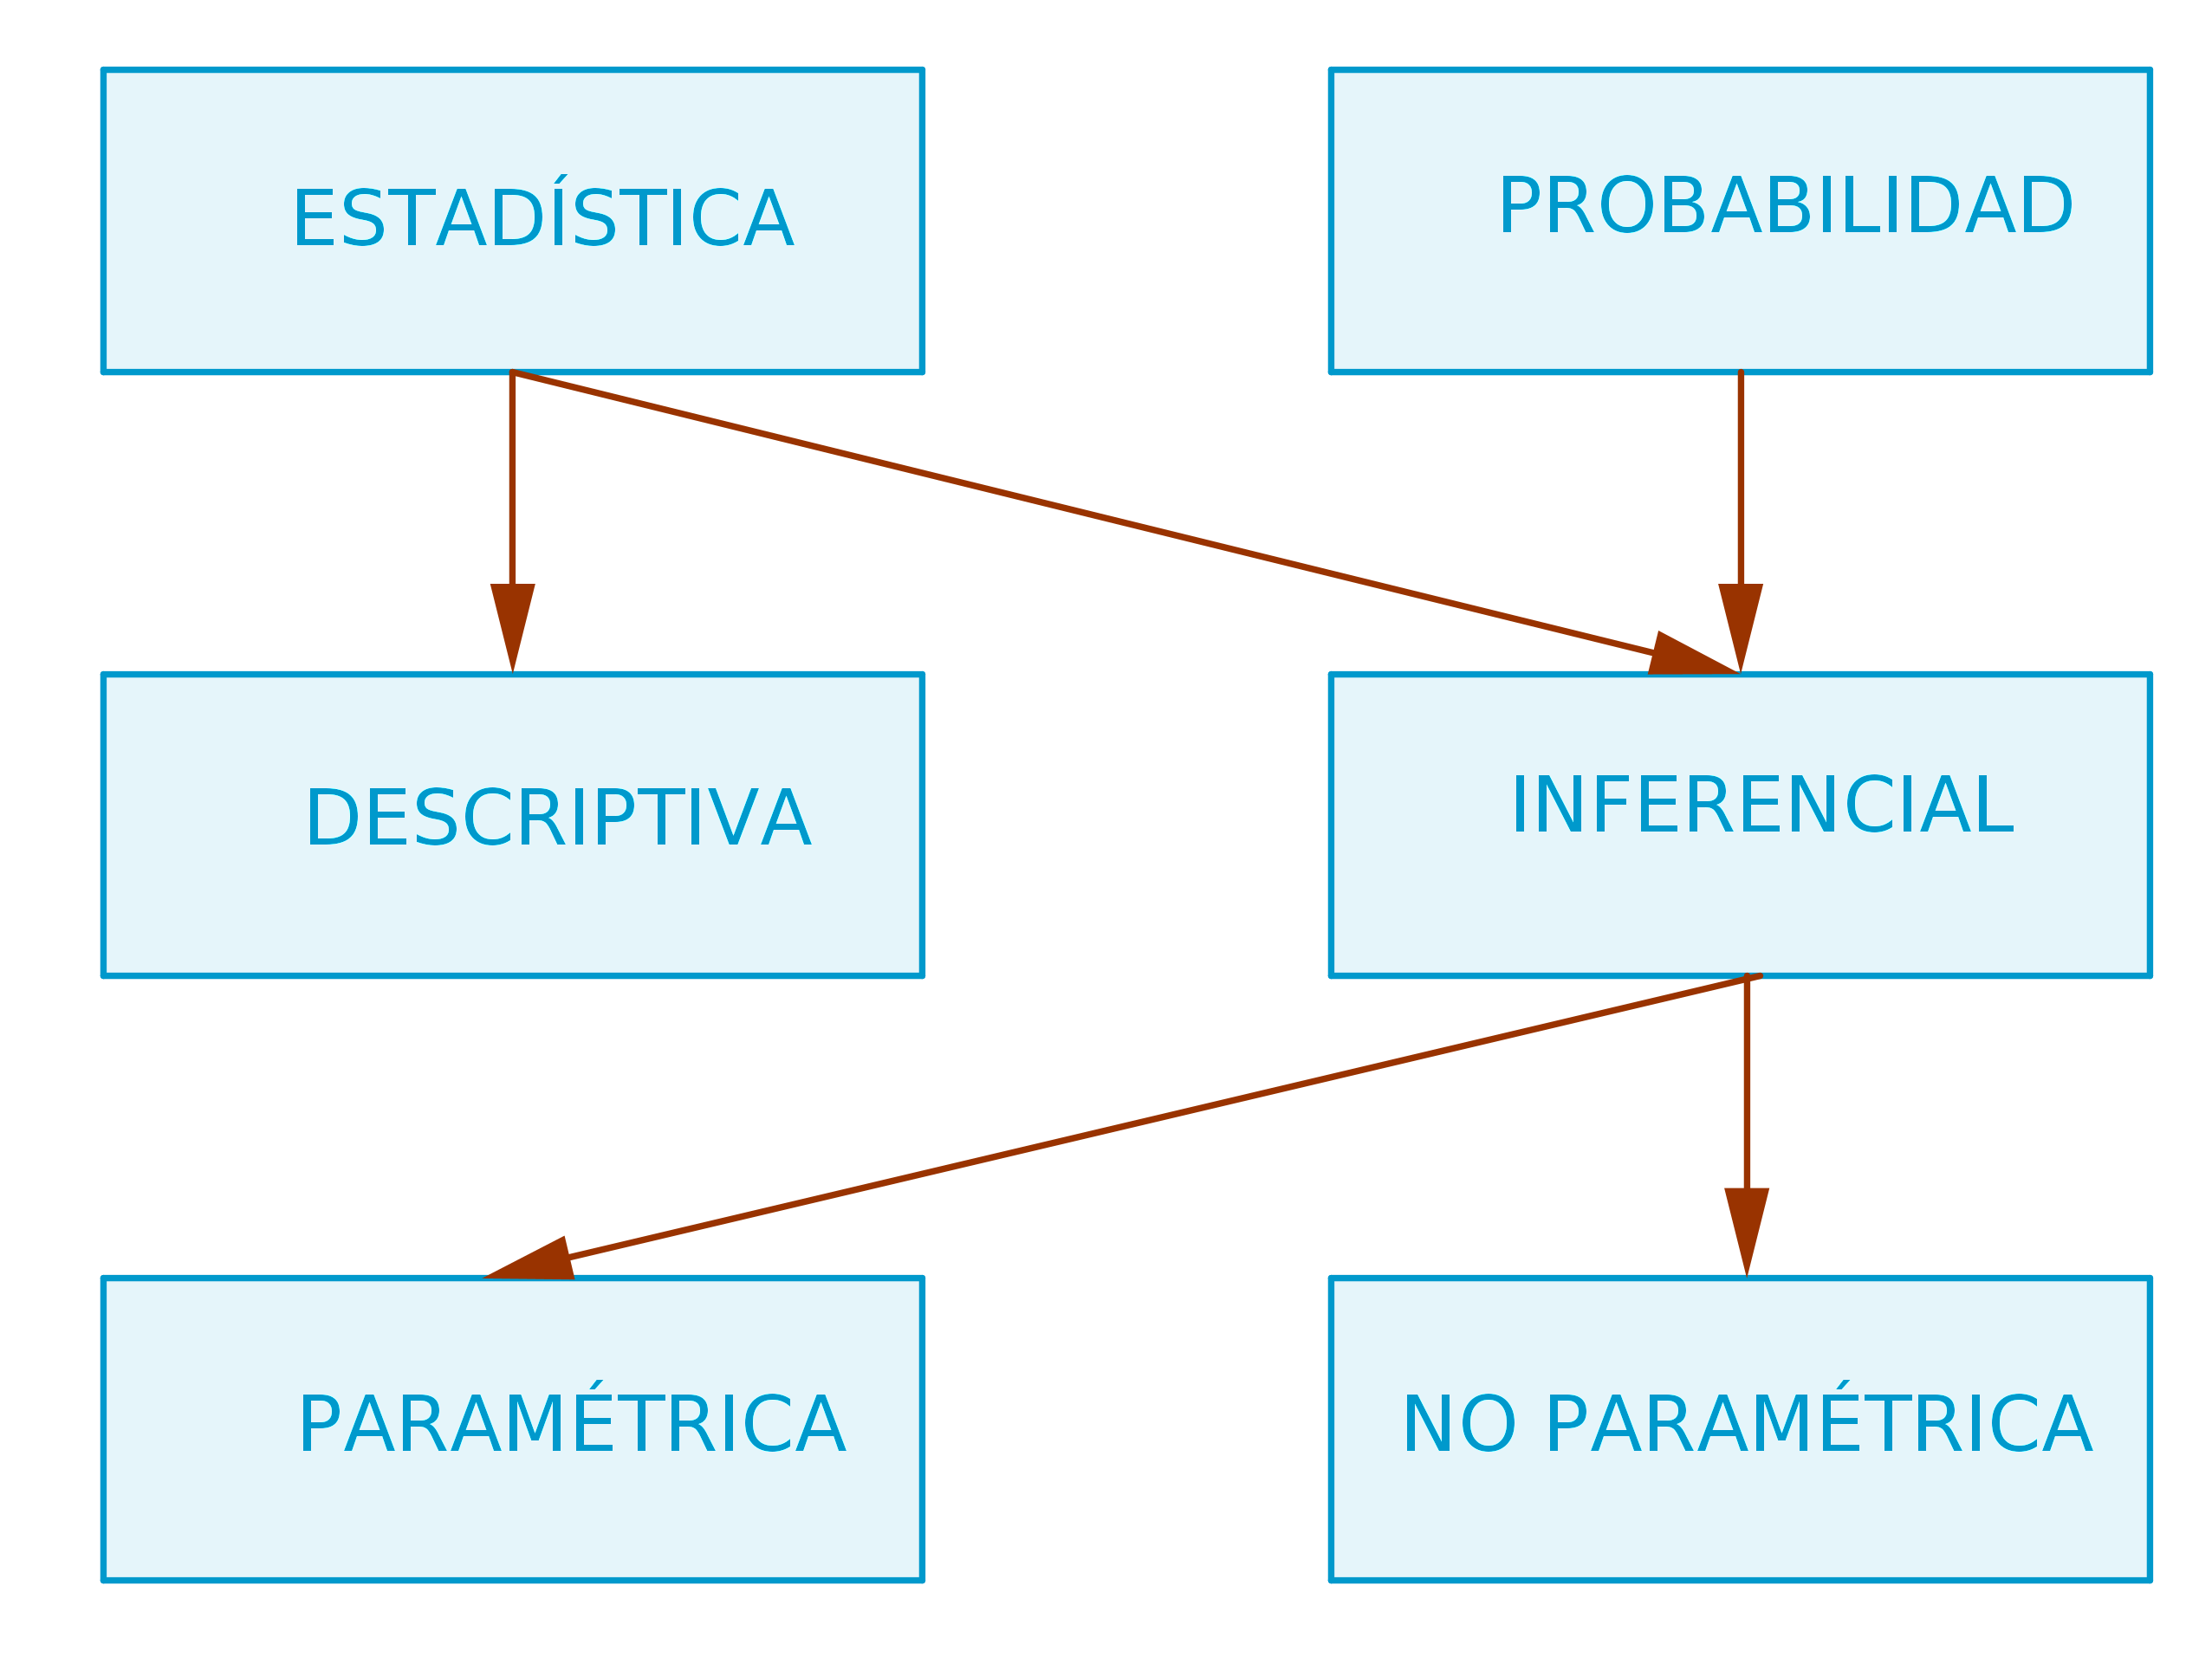
\includegraphics[scale=0.3]{6_home_antalcides_Escritorio_est_libros-est_image_diagrama.png}
\end{figure}


Ahora clasificaremos la estad�stica.

\begin{apunte} \textcolor{zanahoria}{Estad�stica descriptiva:}
Describe y analiza los datos utilizando m�todos num�ricos elementales
y gr�ficos para resumir y presentar la informaci�n contenida en ellos.\index{Estad�stica!desciptiva}
\end{apunte}

\begin{apunte} \textcolor{zanahoria}{Estad�stica inferencial:}
apoy�ndose del c�lculo de pro\-ba\-bilidades y utilizando los datos
de una muestra, efect�a estima\-ciones, decisiones y generaliza sobre
un conjunto mayor de datos llamado poblaci�n.\index{Estad�stica!Inferencial}
\end{apunte}


\section{Conceptos previos}

\begin{defi}{Individuos o elementos:}{def1} Individuos o elementos:Son
personas u objetos que contienen cierta informaci�n de inter�s.\index{Individuos}\index{Elementos}
\end{defi}

\begin{defi}{Poblaci�n:}{def2} Es el conjunto de individuos o elementos
que poseen la misma informaci�n de inter�s, es decir poseen ciertas
propiedades comunes, y lo denotaremos $\Omega.$o $S$\index{Poblaci�n}
\end{defi}

\begin{defi}{Muestra:}{def3} Es un subconjunto representativo de
una poblaci�n.\index{Muestra} \end{defi}

\begin{defi}{Caracteres o atributos:}{def4} Son rasgos o cualidades
de los elementos de la poblaci�n, los cuales pueden ser cualitativos
o cuantitativos.\index{Caracteres} \end{defi}

\begin{defi}{Modalidades:}{def5} Son diferentes situaciones posibles
de un car�cter, los cuales deben ser mutuamente excluyentes y exhaus\-tivos,
es decir cada elemento posee una y solo una de las modalidades posibles
y un car�cter debe tener todas las modalidades posibles.\index{Modalidades}
\end{defi}

\begin{defi}{Clases:}{def6} Conjunto de una o m�s modalidades en
el que se verifica que cada modalidad pertenece a una y solo una de
las clases\index{Clases} \end{defi}

\begin{defi}{Variabilidad:}{def7} Al estudiar unos individuos escogemos
uno varios caracteres, pero la medida de le los caracteres presentan
desviaciones con respecto a una modalidad cuando cada car�cter es
analizado con las mismas condiciones, pero con la imposibilidad de
controlar esas desviaciones. A cada una de esas desviaciones se le
llama variabilidad.\index{Variabilidad} \end{defi}


\subsection{Variables estad�sticas\index{Variables estad�sticas}}

Cuando hablamos de variables estamos en realidad hablando de una funci�n
definida:
\[
f\,:\,\begin{array}{ccc}
A & \longrightarrow & B\\
x_{i} & \longmapsto & X(x_{i})
\end{array}
\]


Donde $A\subseteq\Omega$ y $B$ es un conjunto determinado de modalidades.

Al conjunto $B$ se le denomina dominio de la variable o rango, de
acuerdo con el tipo de dominio las variables se clasifican en:

\begin{defi}{Variables cualitativas:}{def8} Son aquellas que las
modali\-dades posibles son de tipo nominal o categ{�}rico. \end{defi}

\begin{ejemplo} \{si, no\}, \{hombre, mujer\}, \{blanco, negro, amari\-llo,...,etc.\}\index{Varibles!cualitativas}
\end{ejemplo}

\begin{defi}{Variables casicuantitativas:}{def9} Son variables de
tipo nominal, pero se puede establecer un orden entre ellas. \end{defi}

\begin{ejemplo} \{1${^{o}}$,2${^{o}}$,3${^{o}}$,...\}, \{alto,
medio, bajo\}\index{Variables!Cuasicuantitativas} \end{ejemplo}

\begin{defi}{Variables cuantitativas:}{def10} Son las que tienen
por modalidades un conjunto de elementos dotados de operaciones y
estas a su vez se clasifican en discretas y continuas\index{Variables!cuantitativas}
\end{defi}

\begin{defi}{Discretas:}{def11} Cuando las variables toman valores
puntuales \end{defi}

\begin{ejemplo} Cuando el rango es subconjunto de los n\'umeros\ \nz, %\gz o \qz,%
\index{Variables@Discretas} \end{ejemplo}

\begin{defi}{Continuas:}{def12} si $X$ toma todos los valores en
un intervalo \end{defi}

\begin{ejemplo} si $X$ \ $\in\rz$
\end{ejemplo}


\section{Organizaci�n de datos}

Generalmente los datos se organizan usando tablas \ y determinando
algunas cantidades o valores que definiremos a continuaci�n:

Consideremos una poblaci�n finita de $n$ elementos o indivi\-duos
descrita seg�n un car�cter o variable $X$ cuyas modalidades han sido
agrupadas en un n�mero $k$ de clases, que denotaremos $\ c_{1},c_{2},c_{3},...,c_{k}$
y para cada clase $c_{i},i=1,2,3,...,k$ definimos lo si\-guiente:
\footnotetext{La poblaci�n tambi�n puede ser infinita, pero ese caso
lo estudiaremos m�s adelante en el cap�tulo 3}

\begin{defi}{Distribuci�n de frecuencias:}{def17} Es una funci�n
que a cada clase $c_{i}$ de $C$ (el conjunto de todas las clases)
le asigna un valor $n_{i}\in\nz _{0}$,
 es decir, es una funci�n de la forma 
\[
\begin{array}{cccc}
\mathfrak{F}: & C & \rightarrow & \nz_{0}\\
 & c_{i} & \longmapsto & n_{i}
\end{array}
\]


\index{Distribuci�n de frecuencia}

tal que $\mathfrak{F(}c_{i}\mathfrak{)=}n_{i}$

\end{defi}

La funci�n de distribuci�n no es �nica existen cuatro, las cuales
definiremos ahora.

\begin{defi}{ Frecuencia absoluta:}{def13} La frecuencia absoluta
de una clase $c_{i}$ es el n�mero de veces $n_{i}$ que se observa
una modalidad perteneciente a esa clase.\index{Frecencia!Absoluta}
\end{defi}

\begin{defi}{Frecuencia relativa:}{def14} La frecuencia relativa
de una clase $c_{i}$ es el cociente $f_{i}$ entre la frecuencia
absoluta de la clase $c_{i}$ y el n�mero total de observaciones de
todas las modalidades pertenecientes a todas las clases. \end{defi}

Generalmente esta frecuencia se multiplica por 100 y se da en porcentaje\index{Frecuencia!Relativa}

\begin{defi}{Frecuencia absoluta acumulada:}{def15} La frecuencia
absoluta acumulada $N_{i}$ es el n�mero de elementos de la poblaci�n
cuya modalidad es inferior o equivalente a la modalidad $c_{i}$ es
decir,\index{Frecuencia!Absoluta!Acumulada} 
\[
N_{i}=\sum_{j=1}^{k}n_{j}
\]


\end{defi}

\begin{defi}{Frecuencia relativa acumulada:}{def16} Se denota $F_{i}$
y es el tanto por uno de los elementos de la poblaci�n que est�n en
alguna de las clases y que presenta una modalidad inferior o igual
a la $c_{i}$, es decir 
\[
F_{i}=\frac{N_{i}}{n}=\sum_{j=1}^{k}f_{j}
\]


\end{defi}

De �stas definiciones se pueden deducir algunas propiedades evi\-dentes
ya que las modalidades son exhaustivas y mutuamente excluyentes 
\begin{itemize}
\item 
\[
n=\sum_{j=1}^{k}n_{j},
\]

\item 
\[
\sum_{j=1}^{k}f_{j}=1
\]
$\index{Frecuencia!Relativa!Acumulada}$ 
\end{itemize}
\begin{defi}{Tabla de frecuencia:}{def18} Es una representaci�n de
$\mathfrak{F}$ y generalmente una tabla como se muestra en la tabla
\ref{tab1}

\index{Tabla de frecuencias}

Donde:
\begin{itemize}
\item M: representa modalidades, 
\item F.A.: frecuencia absoluta,
\item F.R.: frecuencia relativa, 
\item F.A.A: frecuencia absoluta acumulada y 
\item F.R.A.: frecuencia relativa acumulada.
\end{itemize}
\end{defi}

\begin{table}[H]
\centering\caption{Tabla de Frecuencias\label{tab1}}
 %
\begin{tabular}{|ccccc|}
\arrayrulecolor{ptctitle}\cellcolor{ptctitle!50}{\small{}M}  &
\cellcolor{ptctitle!50}{\small{}F.}  &
\cellcolor{ptctitle!50}{\small{}F.R.}  &
\cellcolor{ptctitle!50}{\small{}F.A.A.}  &
\cellcolor{ptctitle!50}{\small{}F.R.A.}\tabularnewline
\cellcolor{ptcbackground}{\small{}C}  &
\cellcolor{ptcbackground}{\small{}n}$_{i}$  &
\cellcolor{ptcbackground}{\small{}f}$_{i}$  &
\cellcolor{ptcbackground}{\small{}N}$_{i}$  &
\cellcolor{ptcbackground}{\small{}F}$_{i}$\tabularnewline
\cellcolor{gray!50}{\small{}c}$_{1}$  &
\cellcolor{gray!50}{\small{}n}$_{1}$  &
\cellcolor{gray!50}{\small{}f}$_{1}${\small{}=}$\frac{n_{1}}{n}$  &
\cellcolor{gray!50}{\small{}N}$_{1}${\small{}=n}$_{1}$  &
\cellcolor{gray!50}{\small{}F}$_{1}${\small{}=}$\frac{N_{1}}{n}${\small{}=f}$_{1}$\tabularnewline
\cellcolor{ptcbackground}{\small{}Cc}$_{2}$  &
\cellcolor{ptcbackground}{\small{}n}$_{2}$  &
\cellcolor{ptcbackground}{\small{}f}$_{2}${\small{}=}$\frac{n_{2}}{n}$  &
\cellcolor{ptcbackground}{\small{}N}$_{2}${\small{}=n}$_{1}${\small{}+n}$_{2}$  &
\cellcolor{ptcbackground}{\small{}F}$_{2}${\small{}=f}$_{1}${\small{}+f}$_{2}$\tabularnewline
\cellcolor{gray!50}{\small{}c}$_{3}$  &
\cellcolor{gray!50}{\small{}n}$_{3}$  &
\cellcolor{gray!50}{\small{}f}$_{3}${\small{}=}$\frac{n_{3}}{n}$  &
\cellcolor{gray!50}{\small{}N}$_{3}${\small{}=n}$_{1}${\small{}+n}$_{2}${\small{}+n}$_{3}$  &
\cellcolor{gray!50}{\small{}F}$_{3}${\small{}=f}$_{1}${\small{}+f}$_{2}${\small{}+f}$_{3}$\tabularnewline
\cellcolor{ptcbackground}$\vdots$  &
\cellcolor{ptcbackground}$\vdots$  &
\cellcolor{ptcbackground}$\vdots$  &
\cellcolor{ptcbackground}$\vdots$  &
\cellcolor{ptcbackground}$\vdots$\tabularnewline
\cellcolor{gray!50}{\small{}c}$_{j}$  &
\cellcolor{gray!50}{\small{}n}$_{j}$  &
\cellcolor{gray!50}{\small{}f}$_{j}${\small{}=}$\frac{n_{j}}{n}$  &
\cellcolor{gray!50}{\small{}N}$_{j}${\small{}=}$\sum_{i=1}^{j}${\small{}n}$_{i}$  &
\cellcolor{gray!50}{\small{}F}$_{j}${\small{}=}$\sum_{i=1}^{j}${\small{}f}$_{i}$\tabularnewline
\cellcolor{ptcbackground}$\vdots$  &
\cellcolor{ptcbackground}$\vdots$  &
\cellcolor{ptcbackground}$\vdots$  &
\cellcolor{ptcbackground}$\vdots$  &
\cellcolor{ptcbackground}$\vdots$\tabularnewline
\cellcolor{gray!50}{\small{}c}$_{k}$  &
\cellcolor{gray!50}{\small{}n}$_{k}$  &
\cellcolor{gray!50}{\small{}f}$_{k}${\small{}=}$\frac{n_{k}}{n}$  &
\cellcolor{gray!50}{\small{}N}$_{k}${\small{}=n}  &
\cellcolor{gray!50}{\small{}F}$_{k}${\small{}=1}\tabularnewline
\cellcolor{ptcbackground}\footnote{Aunque hemos definido la tabla s�lo para $\mathfrak{F}$ en realidad
en una tablas de frecuencia se tabulan las otras frecuencias definidas
en este apartado}  &
\cellcolor{ptcbackground}{\small{}n}  &
\cellcolor{ptcbackground}{\small{}1}  &
\cellcolor{ptcbackground} &
\cellcolor{ptcbackground}\tabularnewline
\end{tabular}
\end{table}


\begin{ejemplo} Se lanzan cinco monedas 1000 veces. El n�mero de
lanzamientos en los que han salido 0,1,2,3,4,5 caras se indican en
la Tabla \ref{tab:Lanzamiento-de-monedas}: 

\begin{table}[H]
\centering\caption{Lanzamiento de monedas\label{tab:Lanzamiento-de-monedas}}
\begin{tabular}{cllll}
\arrayrulecolor{ptctitle}\cellcolor{ptctitle!50}N\ensuremath{{^{o}}} de caras  &\cellcolor{ptctitle!50}  \ensuremath{n_{i}}  &\cellcolor{ptctitle!50}  \ensuremath{f_{i}}  & \cellcolor{ptctitle!50} \ensuremath{N_{i}}  & \cellcolor{ptctitle!50} \ensuremath{F_{i}}\\
 \cellcolor{ptcbackground} 0  &\cellcolor{ptcbackground}  38  & \cellcolor{ptcbackground}  &  \cellcolor{ptcbackground} & \cellcolor{ptcbackground} \\
 \cellcolor{gray!50} 1  & \cellcolor{gray!50} 144  &  \cellcolor{gray!50} &  \cellcolor{gray!50} & \cellcolor{gray!50} \\
 \cellcolor{ptcbackground} 2  & \cellcolor{ptcbackground} 342  &\cellcolor{ptcbackground}   & \cellcolor{ptcbackground}  & \cellcolor{ptcbackground} \\
 \cellcolor{gray!50} 3  & \cellcolor{gray!50} 287  &\cellcolor{gray!50}   & \cellcolor{gray!50}  & \cellcolor{gray!50} \\
 \cellcolor{ptcbackground} 4  &  \cellcolor{ptcbackground}164  & \cellcolor{ptcbackground}  & \cellcolor{ptcbackground}  & \cellcolor{ptcbackground} \\
 \cellcolor{gray!50} 5  & \cellcolor{gray!50} 25  &\cellcolor{gray!50}   & \cellcolor{gray!50}  & \cellcolor{gray!50} \\
 \cellcolor{ptcbackground}Total  & \cellcolor{ptcbackground} 1000  & \cellcolor{ptcbackground}  &  \cellcolor{ptcbackground} & \cellcolor{ptcbackground} \\
 \end{tabular}
\end{table}

\begin{description}
\item [{{a}.}] Completar la tabla 
\item [{{b}.}] Determinar para que clase \ $F_{i}$ es mayor que el
60\%: $\ F_{\_\_\_}=$\_\_\_ 
\end{description}
\end{ejemplo} 


\subsubsection{Elecci�n de clases}

Las clases se pueden seleccionar de diferentes formas, pero siempre
hay que seguir los criterios que se ajustan al tipo de variables que
estudiamos. 
\begin{itemize}
\item Cuando se trata de una variable nominal las clases $c_{i}$ ser�n
de tipo nominal 
\item Cuando la variable es cuantitativa discreta las clases ser�n valo\-res
num�ricos del tipo $x_{1},x_{2},x_{3},\cdots,x_{k}.$ 
\item Si las variables son cuantitativas continuas las clases se definen
mediante intervalos abiertos o semiabiertos, es decir de la forma:
\[
\left(x_{i-1},x_{i}\right),\left(x_{i},x_{i+1}\right),\left[x_{i-1},x_{i}\right),\left[x_{i},x_{i+1}\right),\left(x_{i-1},x_{i}\right],\left(x_{i},x_{i+1}\right].
\]

\end{itemize}
En estos casos las modalidades que contienen una clase son todos los
valores num�ricos posibles contenidos en el intervalo.

Por convenci�n nosotros de aqu� en adelante tomaremos siempre los
$(k-1)$ primeros intervalos de la forma $\left(x_{i-1},x_{i}\right]$
y el �ltimo $[x_{k-1},x_{k}].$ A cada intervalo lo representaremos
$x_{i-1}-x_{i}=I_{i}$.

\begin{defi}{Amplitud:}{def19} La amplitud de un intervalo se define
$a_{i}=x_{i}-x_{i-1}.$ \end{defi}

\begin{defi}{Marca de clase: }{def20} Es un valor $m_{i}$ $\in I_{i\text{ }}$que
representa a la clase y se define 
\[
m_{i}=\frac{x_{i}+x_{i-1}}{2}
\]


\end{defi}

La marca de clase es una forma abreviada de representar la clase.

\begin{apunte} $m_{i}$ se determina de esta forma si las clases
son conjuntos acotados.\end{apunte}


\subsubsection{Elecci�n de clases para variables continuas}

\index{Clases}Cuando tenemos una muestra es importante escoger en
una forma adecuada las clases y el n�mero de clases $k$ y para ello
indicaremos los siguientes pasos: 
\begin{itemize}
\item Lo primero es determinar $k$, entre mayor sea su valor mejor\footnote{Se aconseja que se escojan entre 5 y 20 clases dependiendo del n�mero
de datos}, pero de todas formas hay que acotarlo por que la idea es reducir
el n�mero de datos en la muestra. 
\[
k=\left\{ \begin{array}{cc}
\sqrt{n} & \text{si }n\text{ es muy grande}\\
1+3.22\log n & \text{en otro caso}
\end{array}\right\} 
\]

\end{itemize}
$n$ se considera grande si $n\geq40$ 
\begin{itemize}
\item Como segundo paso se determina el rango $R=x_{k}-x_{0}$ \index{Rango de la muestra} 
\item Determinado el rango de la muestra podemos hallar la amplitud de cada
intervalo que generalmente la tomamos constante: 
\[
a=\frac{R}{k},\quad a_{i}=a\quad\forall i=1,2,3,...,k
\]
 \index{Amplitud de los intervalos} 
\item Ahora determinaremos los intervalos\footnote{Se aconseja que las marcas de clases coincidan con un gran n�mero
de datos y que los datos no sean extremos de las clases, para que
los c{�}lculos posteriores queden mejor aproximados.} 
\end{itemize}
\begin{align*}
x_{0} & =x_{\min}\\
x_{1} & =x_{0}+a\\
x_{2} & =x_{1}+2a\\
x_{k} & =x_{\max}+ka
\end{align*}


Como se puede observar es posible que el valor de $a$ no sea un n�mero
f�cil de manejar entonces en estos casos como 
\[
x_{k}\geq x_{\max}>x_{\min}\geq x_{0}
\]
 entonces se var�an los extremos sim�tricamente y $a$ se aproxima
al mayor entero es decir $a\prime=\left[\left[a\right]\right]+1$

\begin{ejemplo} Queremos observar el peso de las personas en una
poblaci�n y se toma una muestra de 21 individuos, los cuales est�n
tabulados en la siguiente tabla

$\begin{tabular}{l}
 Peso en Kg\\
 \begin{tabular}{lllllll}
 58  &  42  &  51  &  54  &  40  &  40  &  49\\
 56  &  58  &  57  &  59  &  63  &  58  &  66\\
 70  &  73  &  71  &  69  &  70  &  68  &  64 
\end{tabular} 
\end{tabular}$

Construir la tabla de frecuencias:

\end{ejemplo}

\begin{solucion} Lo primero que hay que identificar es la variable
y en este caso vemos que la variable es de tipo cuantitativa continua
por lo que ahora hay que determinar los intervalos y su longitud para
que la perdida de informaci�n no sea significativa entonces sea $X$
la variable peso, utilizaremos la f�rmula $k=1+3.22\ast\log_{10}21=5.\,\allowbreak257\,5\approxeq6$
aunque podr�amos escoger tambi�n $k=\sqrt{21}\approxeq5$. 

Ahora hallemos $R=73-40=33\Longrightarrow a_{i}=a=\frac{33}{6}=5.\,\allowbreak5$

$x_{0}=x_{\min}=40$

$x_{5}=x_{\max}=73$
\[
\begin{tabular}{||c||c||c||c||c||c||c||}
\hline\hline  \ensuremath{i}  &  Intervalos  &  \ensuremath{m_{i}}  &  \ensuremath{n_{i}}  &  \ensuremath{f_{i}}  &  \ensuremath{N_{i}}  &  \ensuremath{F_{i}}\\
\hline\hline  1  &  40-45,5  &   &   &   &   &  \\
\hline\hline  2  &  45,5-51  &   &   &   &   &  \\
\hline\hline  3  &   &   &   &   &   &  \\
\hline\hline  4  &   &   &   &   &   &  \\
\hline\hline  5  &  62-67.5  &   &   &   &   &  \ensuremath{\thickapprox1}\\
\hline\hline   &   &   &   &   &  21  &  \ensuremath{\thickapprox1}\\
\hline\hline   &   &   &  21  &  \ensuremath{\thickapprox1}  &   &  
\\\hline\hline \end{tabular}
\]


Existe otra posibilidad de construir la tabla y es escogiendo por
ejemplo $a\prime=7\Longrightarrow R\prime=a\prime\cdot5=35$

$d=R\prime-R=2\Longrightarrow x_{0}=x_{\min}-\frac{d}{2}=39,\quad x_{5}=x_{\max}+\frac{d}{2}=74$

\bigskip{}


\begin{center}
\bigskip{}
 $\begin{tabular}{||c||c||c||c||c||c||c||}
\hline\hline  \ensuremath{i}  &  Intervalos  &  \ensuremath{m_{i}}  &  \ensuremath{n_{i}}  &  \ensuremath{f_{i}}  &  \ensuremath{N_{i}}  &  \ensuremath{F_{i}}\\
\hline\hline  1  &  39-46  &   &   &   &   &  \\
\hline\hline  2  &  46-53  &   &   &   &   &  \\
\hline\hline  3  &   &   &   &   &   &  \\
\hline\hline  4  &   &   &   &   &   &  \\
\hline\hline  5  &  67-74  &   &   &   &   &  \\
\hline\hline  6  &   &   &   &   &  21  &  \ensuremath{\thickapprox1}\\
\hline\hline   &   &   &  21  &  \ensuremath{\thickapprox1}  &   &  
\\\hline\hline \end{tabular}$
\par\end{center}

\end{solucion}

Utilizando un software estad�stico \textbf{\textsl{Statgraphics}}
\textregistered,\  obtenemos la siguiente tabla

\begin{center}
\includegraphics[width=11.1017cm,height=6.6009cm]{7_media_antalcides_Antalcides-EXT1_bak-pc_documentos_Libros_LibrosDPTO_est_peso.pdf} 
\par\end{center}

Podemos usar \textcolor{blue}{R} para resolver el ejercicio, en este
caso cargamos el paquete \textsl{\textcolor{blue}{Agricolae}} como
se muestra a continuaci�n




\begin{knitrout}
\definecolor{shadecolor}{rgb}{0.969, 0.969, 0.969}\color{fgcolor}\begin{kframe}
\begin{alltt}
\hlkwd{round}\hlstd{(}\hlkwd{table.freq}\hlstd{(h1),} \hlnum{2}\hlstd{)}
\end{alltt}
\begin{verbatim}
##   Lower Upper Main Frequency Percentage CF   CPF
## 1  40.0  46.6 43.3         3       14.3  3  14.3
## 2  46.6  53.2 49.9         2        9.5  5  23.8
## 3  53.2  59.8 56.5         7       33.3 12  57.1
## 4  59.8  66.4 63.1         3       14.3 15  71.4
## 5  66.4  73.0 69.7         6       28.6 21 100.0
\end{verbatim}
\end{kframe}
\end{knitrout}

\begin{knitrout}
\definecolor{shadecolor}{rgb}{0.969, 0.969, 0.969}\color{fgcolor}\begin{kframe}
\begin{alltt}
\hlkwd{stem}\hlstd{(peso)}
\end{alltt}
\begin{verbatim}
## 
##   The decimal point is 1 digit(s) to the right of the |
## 
##   4 | 0029
##   5 | 14678889
##   6 | 34689
##   7 | 0013
\end{verbatim}
\end{kframe}
\end{knitrout}


\section{Representaciones gr�ficas y diagramas}

En la secci�n anterior hemos visto que al organizar los datos en una
tabla se reduce la informaci�n, pero con ello podemos analizarlos
de manera m�s sistem�tica y de esa manera podemos concentrarnos en
los m�s importante, pero a�n as� a veces no es f�cil observar todo
lo que queremos, sobre todo si la persona interesada en los resultados
no le interesa la estad�stica y sabe muy poco de ella, por lo que
una representaci�n gr�fica simplifica a�n m�s los datos.


\subsection{Gr�ficos para variables cualitativas\index{Diagramas de barra}}
\begin{description}
\item [{{i.}}] Diagramas de barras


Se establece una especie de plano cartesiano representando las modalidades
en el eje de ordenadas y las frecuencias absolutas o relativas en
el eje de las abscisas, con este gr�fico \ si\ se comparan varias
poblaciones entre s� es conveniente utilizar las frecuencias relativas

\end{description}
\begin{flushleft}
Diagrama de barra para una variable cualitativa \label{ec1} 
\par\end{flushleft}
\begin{quote}
\begin{figure}[ph]
\begin{centering}
\includegraphics[width=8.5668cm,height=9.4784cm]{8_media_antalcides_Antalcides-EXT1_bak-pc_documentos_Libros_LibrosDPTO_est_Areac.pdf}\caption{AREAS DE LOS CONTINENTES}

\par\end{centering}

\centering{}\label{ec1} 
\end{figure}


\begin{center}
\includegraphics[width=10.4252cm,height=8.2549cm]{9_media_antalcides_Antalcides-EXT1_bak-pc_documentos_Libros_LibrosDPTO_est_trigom.pdf}\label{ec1} 
\par\end{center}\end{quote}
\begin{description}
\item [{\bigskip{}
}]~
\item [{ii.}] Diagramas circulares o sectores: 
\end{description}
En estos diagramas se toma un c�rculo o cilindro y se dividen en tantos
sectores como clases existan de modo que cada sector es proporcional
a su frecuencia absoluta o acumulada, como se indica en los siguientes
diagramas:

\begin{center}
\includegraphics[width=8.2549cm,height=10.3175cm]{10_media_antalcides_Antalcides-EXT1_bak-pc_documentos_Libros_LibrosDPTO_est_feconomia.pdf}\\
 Diagrama circular 
\par\end{center}

Con estos diagramas tambi�n se pueden comparar dos poblaciones utilizando
dos semic{�}rculos de radios $r_{1}$ y $r_{2}$ tal que $r_{2}>r_{1}$
y cumplan la relaci�n: $r_{2}=r_{1}\sqrt{\frac{n_{2}}{n_{1}}}$ donde
las $n$ representan el tama�o de las poblaciones.

\begin{center}
\includegraphics[width=3.8397cm,height=3.2466cm]{11_media_antalcides_Antalcides-EXT1_bak-pc_documentos_Libros_LibrosDPTO_est_2pob.pdf}\\
 DOS MUESTRAS 
\par\end{center}

\index{Diagramas!Circulares} 
\begin{description}
\item [{iii.}] Pictogramas: Cuando se expresan dibujos alusivos al tema
en estudio estos dibujos se hacen de tal forma que se utilizan diferentes
escalas para representar la frecuencia absoluta o relativa.


\begin{center}
\includegraphics[width=3.6867in,height=1.6553in]{12_media_antalcides_Antalcides-EXT1_bak-pc_documentos_Libros_LibrosDPTO_est_Pictog.pdf} 
\par\end{center}


\index{Pictograma}

\end{description}

\subsection{Gr�ficos para variables cuantitativas}
\begin{description}
\item [{i.}] Diagrama de puntos: En este diagrama se coloca la frecuencia
absoluta o relativa de una modalidad en una recta num�rica y nos sirve
para analizar dos o m�s modalidades cuando el n�mero de datos es peque�o,
con este gr�fico analizamos f�cilmente la tendencia y la variabilidad
de la muestra. lo mismo que caracter�sticas poco usuales.


\begin{center}
\includegraphics[width=3.7446in,height=1.1978in]{13_media_antalcides_Antalcides-EXT1_bak-pc_documentos_Libros_LibrosDPTO_est_punto.pdf} 
\par\end{center}


\index{Diagrama!De puntos}

\item [{ii.}] Diagrama de tallo y hoja: Cuando el conjunto de datos 
\[
x_{1},x_{2},x_{3},\cdots,x_{n}.x_{1},x_{2},x_{3},\cdots,x_{n}.
\]
 es grande cada $x_{i},\quad i=1,2,3,...,n$ tiene m�s de dos d�gitos,
entonces se dividen los $x_{i}$ en dos partes . Un tallo formado
por los primeros d�gitos. Una hoja formada por el resto de d�gitos\index{Diagrama!De tallo y hoja}\begin{ejemplo}
En un examen de clasificaci�n para seleccionar alumnos que pueden
ver directamente c�lculo en el primer semestre en la facultad de ingenier�a
se obtuvieron los siguientes resultados: \end{ejemplo} \ $\left[\begin{array}{cccccccccc}
95 & 95 & 100 & 100 & 100 & 100 & 100 & 105 & 105 & 105\\
110 & 110 & 110 & 110 & 110 & 110 & 110 & 110 & 110 & 115\\
115 & 115 & 115 & 115 & 115 & 115 & 115 & 115 & 115 & 115\\
120 & 120 & 120 & 120 & 120 & 120 & 120 & 120 & 125 & 125\\
125 & 125 & 130 & 130 & 130 & 130 & 135 & 135 & 140 & 140
\end{array}\right]\allowbreak$
\end{description}
$\text{\begin{tabular}{l||llllllllllllllllllll}
 {\tiny09}  &  {\tiny5}  &  {\tiny5}  &  {\tiny-}  &  {\tiny-}  &  {\tiny-}  &  {\tiny-}  &  {\tiny-}  &  {\tiny-}  &  {\tiny-}  &  {\tiny-}  &  {\tiny-}  &  {\tiny-}  &  {\tiny-}  &  {\tiny-}  &  {\tiny-}  &  {\tiny-}  &  {\tiny-}  &  {\tiny-}  &  {\tiny-}  &  {\tiny-}\\
 {\tiny10}  &  {\tiny0}  &  {\tiny0}  &  {\tiny0}  &  {\tiny0}  &  {\tiny0}  &  {\tiny5}  &  {\tiny5}  &  {\tiny5}  &  {\tiny-}  &  {\tiny-}  &  {\tiny-}  &  {\tiny-}  &  {\tiny-}  &  {\tiny-}  &  {\tiny-}  &  {\tiny-}  &  {\tiny-}  &  {\tiny-}  &  {\tiny-}  &  {\tiny-}\\
 {\tiny11}  &  {\tiny0}  &  {\tiny0}  &  {\tiny0}  &  {\tiny0}  &  {\tiny0}  &  {\tiny0}  &  {\tiny0}  &  {\tiny0}  &  {\tiny0}  &  {\tiny5}  &  {\tiny5}  &  {\tiny5}  &  {\tiny5}  &  {\tiny5}  &  {\tiny5}  &  {\tiny5}  &  {\tiny5}  &  {\tiny5}  &  {\tiny5}  &  {\tiny5}\\
 {\tiny12}  &  {\tiny0}  &  {\tiny0}  &  {\tiny0}  &  {\tiny0}  &  {\tiny0}  &  {\tiny0}  &  {\tiny0}  &  {\tiny0}  &  {\tiny5}  &  {\tiny5}  &  {\tiny5}  &  {\tiny5}  &  {\tiny-}  &  {\tiny-}  &  {\tiny-}  &  {\tiny-}  &  {\tiny-}  &  {\tiny-}  &  {\tiny-}  &  {\tiny-}\\
 {\tiny13}  &  {\tiny0}  &  {\tiny0}  &  {\tiny0}  &  {\tiny0}  &  {\tiny5}  &  {\tiny5}  &  {\tiny-}  &  {\tiny-}  &  {\tiny-}  &  {\tiny-}  &  {\tiny-}  &  {\tiny-}  &  {\tiny-}  &  {\tiny-}  &  {\tiny-}  &  {\tiny-}  &  {\tiny-}  &  {\tiny-}  &  {\tiny-}  &  {\tiny-}\\
 {\tiny14}  &  {\tiny0}  &  {\tiny0}  &  {\tiny-}  &  {\tiny-}  &  {\tiny-}  &  {\tiny-}  &  {\tiny-}  &  {\tiny-}  &  {\tiny-}  &  {\tiny-}  &  {\tiny-}  &  {\tiny-}  &  {\tiny-}  &  {\tiny-}  &  {\tiny-}  &  {\tiny-}  &  {\tiny-}  &  {\tiny-}  &  {\tiny-}  &  {\tiny-} 
\end{tabular} }$
\begin{description}
\item [{iii.}] Diagramas diferenciales: Son aquellos en los que se representan
gr�ficamente frecuencias absolutas y relativas \index{Diagramas!Diferenciales} 
\item [{iv.}] Diagramas integrales: Son los diagramas en los que se representan
gr�ficamente el n�mero de elementos que presentan una modalidad inferior
o igual a una modalidad dada y se generan a tr�ves de las frecuencias
acumuladas\index{Diagramas!Integrales} 
\end{description}
Debido a que existen dos tipos de variables cuantitativas entonces
debemos clasificar estos dos tipos de diagramas de acuerdo con el
tipo de variable cuantitativa en estudio.


\paragraph{Gr�ficos para variables discreta}

Al representar gr�ficamente la frecuencia absoluta o relativa de una
variable discreta usamos los diagrama de barras, pero a diferencia
de los diagrama de barra de las variables cualitativas las barras
aqu� se presentan con l{�}neas delgadas, para indicar as� la naturaleza
de la variable. En el caso de los diagramas integrales tienen la forma
del gr�fico de una funci�n escalonada

\begin{ejemplo} La siguiente tabla representa el n�mero de hijos
que ten�an 12 familias encuestadas de un caser�o cerca a Baranoa:
\[
\begin{tabular}{||l||l||l||l||}
\hline\hline  \ensuremath{x_{i}}  &  \ensuremath{n_{i}}  &  \ensuremath{f_{i}}  &  \ensuremath{N_{i}}\\
\hline\hline  1  &  1  &   &  \\
\hline\hline  2  &  3  &   &  \\
\hline\hline  3  &  5  &   &  \\
\hline\hline  4  &  3  &   &  \\
\hline\hline   &  12  &   &  
\\\hline\hline \end{tabular}
\]
 \end{ejemplo} 
\begin{figure}[h]
\centering{}\includegraphics[width=9.5333cm,height=5.0676cm]{14_media_antalcides_Antalcides-EXT1_bak-pc_documentos_Libros_LibrosDPTO_est_barah.pdf}\caption{FRECUENCIAS ABSOLUTAS}
\end{figure}


\begin{center}
\includegraphics[width=7.8024cm,height=6.1505cm]{15_media_antalcides_Antalcides-EXT1_bak-pc_documentos_Libros_LibrosDPTO_est_barah1.pdf}\\
 FRECUENCIAS ABSOLUTAS ACUMULADAS 
\par\end{center}

Para las variables continuas tambi�n se pueden representar con diagramas
circulares

\begin{center}
\begin{ejemplo} La tabla representa las notas obtenidas por los alumnos
de \ 11en un examen de Matem�ticas en 1990 
\begin{equation}
\begin{tabular}{ccc}
\hline  \textbf{Notas}  &  \textbf{Frecuencia}  &  \textbf{\ frecuencia Relativa}\\
\hline  \ensuremath{10\ }  &  \ensuremath{2}  &  \ensuremath{2/15=.133}\\
 \ensuremath{9}  &  \ensuremath{3}  &  \ensuremath{3/15=.200}\\
 \ensuremath{8}  &  \ensuremath{4}  &  \ensuremath{4/15=.267}\\
 \ensuremath{7}  &  \ensuremath{4}  &  \ensuremath{4/15=.267}\\
 \ensuremath{4}  &  \ensuremath{2}  &  \ensuremath{2/15=.133} 
\end{tabular}\tag{Tabla 1}
\end{equation}
 
\begin{equation}
\begin{tabular}{cccccccccc}
\hline  \textbf{notas}  &  \ensuremath{\mathbf{n}_{i}}  &   &  \textbf{f}\ensuremath{_{i}}  &   &  \ensuremath{f_{i}} \textbf{\%}  &   &  \ensuremath{\mathbf{N}_{i}}  &   &  \ensuremath{\mathbf{F}_{i}}\\
\hline  \ensuremath{10\ }  &  \ensuremath{2}  &   &  \ensuremath{2/15=.133}  &   &  \ensuremath{13.3}  &   &  \ensuremath{15}  &   &  \ensuremath{1.000}\\
 \ensuremath{9}  &  \ensuremath{3}  &   &  \ensuremath{3/15=.200}  &   &  \ensuremath{20.0}  &   &  \ensuremath{13}  &   &  \ensuremath{.867}\\
 \ensuremath{8}  &  \ensuremath{4}  &   &  \ensuremath{4/15=.267}  &   &  \ensuremath{26.7}  &   &  \ensuremath{10}  &   &  \ensuremath{.667}\\
 \ensuremath{7}  &  \ensuremath{4}  &   &  \ensuremath{4/15=.267}  &   &  \ensuremath{26.7}  &   &  \ensuremath{6}  &   &  \ensuremath{.400}\\
 \ensuremath{4}  &  \ensuremath{2}  &   &  \ensuremath{2/15=.133}  &   &  \ensuremath{13.3}  &   &  \ensuremath{2}  &   &  \ensuremath{.133} 
\end{tabular}\tag{Tabla 2}
\end{equation}
\end{ejemplo} \fbox{\includegraphics[width=6.4449cm,height=5.9814cm]{16_media_antalcides_Antalcides-EXT1_bak-pc_documentos_Libros_LibrosDPTO_est_chart4.pdf}} 
\par\end{center}


\paragraph{Gr�ficos para variables continuas}

Para las variables continuas existen dos tipos de gr�ficos: 
\begin{itemize}
\item Los histogramas: Los cuales se construyen representando sobre cada
intervalo, un rect�ngulo que tiene la longitud del segmento como base
y la altura debe ser un valor proporcional a el valor de la frecuencia
para ese intervalo.\index{Histogramas} 
\item Pol�gono de frecuencias: Este se elabora uniendo los puntos que corresponden
a las im�genes de las marcas de clase. 
\end{itemize}
En el caso de los diagramas integrales a estos pol�gonos se les llama
ojiva y se obtienen uniendo las abscisas a partir de los extremos
de los intervalos en los que se han organizado los datos

\begin{ejemplo} Representar gr�ficamente la informaci�n que apare\-ce
en la siguiente tabla \end{ejemplo}

\begin{center}
\begin{tabular}{||c||c||c||c||}
\hline 
Intervalos  &
$m_{i}$  &
$n_{i}$  &
$N_{i}$\tabularnewline
\hline 
\hline 
0-2  &
1  &
1  &
\tabularnewline
\hline 
\hline 
2-4  &
3  &
4  &
\tabularnewline
\hline 
\hline 
4-6  &
5  &
10  &
\tabularnewline
\hline 
\hline 
6-8  &
7  &
3  &
\tabularnewline
\hline 
\hline 
8-10  &
9  &
1  &
\tabularnewline
\hline 
\hline 
 &
 &
 &
\tabularnewline
\hline 
\end{tabular}
\par\end{center}

\begin{center}
\includegraphics[width=6.7173cm,height=5.0676cm]{17_media_antalcides_Antalcides-EXT1_bak-pc_documentos_Libros_LibrosDPTO_est_hisc.pdf}\\
 Diagrama Diferencial 
\par\end{center}

\begin{center}
\includegraphics[width=7.3916cm,height=5.4191cm]{18_media_antalcides_Antalcides-EXT1_bak-pc_documentos_Libros_LibrosDPTO_est_poligono.pdf}\\
 Pol�gono de frecuencias 
\par\end{center}

\begin{center}
\includegraphics[width=7.9298cm,height=5.3773cm]{19_media_antalcides_Antalcides-EXT1_bak-pc_documentos_Libros_LibrosDPTO_est_Acumu.pdf}\\
 Diagrama acumulado 
\par\end{center}

\begin{ejemplo} Representar gr�ficamente los datos de la tabla1 
\begin{equation}
\begin{tabular}{cc}
\hline  \textbf{\label{Table1}Notas}  &  \textbf{Frecuencia}\\
\hline  \ensuremath{10\ }  &  \ensuremath{2}\\
 \ensuremath{9}  &  \ensuremath{3}\\
 \ensuremath{8}  &  \ensuremath{4}\\
 \ensuremath{7}  &  \ensuremath{4}\\
 \ensuremath{6}  &  \ensuremath{0}\\
 \ensuremath{5}  &  \ensuremath{0}\\
 \ensuremath{4}  &  \ensuremath{2}\\
 \ensuremath{3}  &  \ensuremath{0}\\
 \ensuremath{2}  &  \ensuremath{0}\\
 \ensuremath{1}  &  \ensuremath{0}\\
 \ensuremath{0}  &  \ensuremath{0} 
\end{tabular}\tag{Tabla 1}
\end{equation}


\end{ejemplo}

\bigskip{}
 
\begin{figure}[ptb]
\centering{}\includegraphics[width=4.3448in,height=2.7795in]{20_media_antalcides_Antalcides-EXT1_bak-pc_documentos_Libros_LibrosDPTO_est_notas.pdf} 
\end{figure}


\begin{center}
\includegraphics[width=3in,height=2.0003in]{21_media_antalcides_Antalcides-EXT1_bak-pc_documentos_Libros_LibrosDPTO_est_H0CZ9D00.pdf}\\
 Test Scores 
\par\end{center}

\begin{center}
\includegraphics[width=4.1459in,height=2.4232in]{22_media_antalcides_Antalcides-EXT1_bak-pc_documentos_Libros_LibrosDPTO_est_H0CZA601.pdf}\\
 Test Scores 
\par\end{center}
\begin{description}
\item [{{{*}}}] Realizar una ojiva que represente los datos de la tabla2 \end{description}
\begin{itemize}
\item Diagrama de caja: El diagrama de caja es una representaci�n visual
que describe varias caracter�sticas importantes tales coma \ son:
la dispersi�n, la variabilidad, la simetr�a e identifica los datos
que se alejan de manera poco usual del resto de los datos. 
\end{itemize}
En un diagrama de caja se concentran el 50\% de los datos en un rect�ngulo,
ubicando los valores para los cuales la frecuencia relativa acumulada
son el 25\% y el 75\% respectivamente en l�neas horizontales o verticales
formando los lados paralelos del rect�ngulo, tambi�n se utiliza una
l�nea que pasa por el centro del rect�ngulo para representar el dato
que le corresponde a la frecuencia relativa acumulada del 50\%. De
los dos lados del rect�ngulo antes mencionados se extiende una l�nea
perpendicular hasta los extremos m�s alejados, los valores que se
encuentran en esta regi�n se llaman valores at�picos o extremos.

\begin{ejemplo} La siguiente tabla muestra los datos sobre la viscosidad
de tres mezclas \end{ejemplo}

\begin{center}
\bigskip{}
 %
\begin{tabular}{lll}
\hline 
mezcla 1  &
mezcla 2  &
mezcla 2\tabularnewline
\hline 
22.02  &
21.49  &
20.33\tabularnewline
23.83  &
22.67  &
21.67\tabularnewline
26.67  &
24.62  &
24.67\tabularnewline
25.38  &
24.18  &
22.45\tabularnewline
25.48  &
22.78  &
22.28\tabularnewline
23.50  &
22.56  &
21.95\tabularnewline
25.90  &
24.46  &
20.49\tabularnewline
24.98  &
23.79  &
21.81\tabularnewline
\hline 
\end{tabular}
\par\end{center}

\bigskip{}


\begin{center}
\includegraphics[width=3.25in,height=2.0046in]{23_media_antalcides_Antalcides-EXT1_bak-pc_documentos_Libros_LibrosDPTO_est_dcaja.pdf} 
\par\end{center}
\begin{itemize}
\item Gr�ficas de serie de tiempo: Estas gr�ficas de series de tiempo se
utilizan cuando nos interesa averiguar si el momento en que se tomaron
afecta su variabilidad. 
\end{itemize}
\begin{ejemplo} El n�mero de piezas (en miles) existentes en el almac�n
de una determinada f�brica el �ltimo d�a de cada mes del a�o 1981,
viene dado por la tabla\\
 %
\begin{tabular}{lllllllllllll}
{\tiny{}Meses}  &
{\tiny{}Ene.}  &
{\tiny{}Feb.}  &
{\tiny{}Mar.}  &
{\tiny{}Abr.}  &
{\tiny{}Ma..}  &
{\tiny{}Jun.}  &
{\tiny{}Jul.}  &
{\tiny{}Ag.}  &
{\tiny{}Sep.}  &
{\tiny{}Oct.}  &
{\tiny{}Nov.}  &
{\tiny{}Dic.}\tabularnewline
{\tiny{}Piezas}  &
{\tiny{}5,5}  &
{\tiny{}6,3}  &
{\tiny{}6,6}  &
{\tiny{}7}  &
{\tiny{}7}  &
{\tiny{}7,5}  &
{\tiny{}8,5}  &
{\tiny{}8}  &
{\tiny{}8,3}  &
{\tiny{}7,5}  &
{\tiny{}7}  &
{\tiny{}6}\tabularnewline
\end{tabular}

\end{ejemplo}

\bigskip{}


\begin{center}
\includegraphics[scale=0.2]{24_media_antalcides_Antalcides-EXT1_bak-pc_documentos_Libros_LibrosDPTO_est_serie.pdf}
\par\end{center}


\subsubsection{Diagrama de Tallo y Hoja}

Salida del programa estad�stico \textbf{\textsl{Statgraphics}} \textregistered,\ 
para el peso de las 27 personas

\textbf{\textcolor{black}{Diagrama de Tallo y Hoja para Peso: unidad
= 1,0 \ \ 1{\textbar}2 representa 12,0}}

\bigskip{}


\textcolor{black}{\ \ \ \ \ \ 3 \ \ \ \ 4{\textbar}002}

\textcolor{black}{\ \ \ \ \ \ 5 \ \ \ \ 4{\textbar}99}

\textcolor{black}{\ \ \ \ \ \ 7 \ \ \ \ 5{\textbar}14}

\textcolor{black}{\ \ \ \ (10) \ \ 5{\textbar}6778888899}

\textcolor{black}{\ \ \ \ \ 10 \ \ \ \ 6{\textbar}3334}

\textcolor{black}{\ \ \ \ \ \ 6 \ \ \ \ 6{\textbar}689}

\textcolor{black}{\ \ \ \ \ \ 3 \ \ \ \ 7{\textbar}001}

\bigskip{}


\textcolor{black}{Este diagrama muestra la tabulaci�n de frecuencias
para Peso. \ El rango de los datos se ha dividido en 7 intervalos
(llamados tallos), cada uno representado por un rengl�n en la tabla.
\ Los tallos se etiquetan utilizando uno � m�s d�gitos indicadores
para los valores que caen dentro de ese intervalo. \ En cada rengl�n,
los valores individuales se representan por un d�gito (llamado hoja)
a la derecha de la l�nea vertical. \ Esto resulta en un histograma
para los datos del cual uno puede recuperar, al menos, dos d�gitos
significativos de cada valor. \ Si hay algunos puntos muy alejados
del resto (llamados puntos lejanos), se colocan en tallos alto y bajo
separados. \ En este caso, no hay puntos alejados}

Salida obetnida con \textcolor{blue}{R} para el mismo ejemplo

\begin{knitrout}
\definecolor{shadecolor}{rgb}{0.969, 0.969, 0.969}\color{fgcolor}\begin{kframe}
\begin{alltt}
\hlkwd{stem}\hlstd{(peso)}
\end{alltt}
\begin{verbatim}
## 
##   The decimal point is 1 digit(s) to the right of the |
## 
##   4 | 0029
##   5 | 14678889
##   6 | 34689
##   7 | 0013
\end{verbatim}
\end{kframe}
\end{knitrout}

\problemas{ 
\begin{enumerate}
\item Decir si los datos que representan \ los siguientes item son continuos
o,discretos o cualitativos

\begin{enumerate}
\item Color de los ojos 
\item Letras usadas en un p�rrafo 
\item Velocidad de un coche 
\item Edad de un trabajador 
\item N�mero de billetes de 20000 que circulan en una ciudad 
\item N�mero de estudiantes matriculados en la Universidad 
\item Caudal del r�o,medido en diferentes d�as del a�o 
\end{enumerate}
\item El conjunto de datos adjunto est� formado de observaciones del gasto
de agua en regaderas (L/min) para una muestra de $n=128$ casas \ de
un sector exclusivo de Barranquilla\\
 \\
\hspace*{-10pt} $\begin{array}{cccccccccc}
4.6 & 12.3 & 7.1 & 4.0 & 9.2 & 6.7 & 6.9 & 11.5 & 5.1 & 3.8\\
11.2 & 10.5 & 14.3 & 8.0 & 8.8 & 6.8 & 5.1 & 5.6 & 9.6 & 7.5\\
7.5 & 6.2 & 5.8 & 2.3 & 3.4 & 10.4 & 9.8 & 6.6 & 3.7 & 6.4\\
6.0 & 8.3 & 6.5 & 7.6 & 9.3 & 9.2 & 7.3 & 5.0 & 6.3 & 13.8\\
6.2 & 5.4 & 4.8 & 7.5 & 6.0 & 6.9 & 10.8 & 7.5 & 6.6 & 5.5\\
3.3 & 7.6 & 3.9 & 11.9 & 2.2 & 15.0 & 7.2 & 6.1 & 15.3 & 18.9\\
7.2 & 5.4 & 5.5 & 4.3 & 9.0 & 12.7 & 11.5 & 7.4 & 5.0 & 3.5\\
8.2 & 8.4 & 7.3 & 10.3 & 11.9 & 6.0 & 5.6 & 9.5 & 9.3 & 10.4\\
9.7 & 5.1 & 6.7 & 10.2 & 6.2 & 8.4 & 7.0 & 4.8 & 5.6 & 10.5\\
14.6 & 10.8 & 15.5 & 7.5 & 6.4 & 3.4 & 5.5 & 6.6 & 5.9 & 15.0\\
9.6 & 7.8 & 7.0 & 6.9 & 4.1 & 3.5 & 11.9 & 3.7 & 5.7 & 6.8\\
11.3 & 9.3 & 9.6 & 10.4 & 9.3 & 6.9 & 9.8 & 9.1 & 10.6 & 4.5\\
6.2 & 8.3 & 3.2 & 4.9 & 5.0 & 6.0 & 8.2 & 6.3
\end{array}$\\


\begin{enumerate}
\item Dibuje un histograma de frecuencias absolutas en el eje vertical 
\item Dibuje un diagrama acumulado 
\item Construya una representaci�n de tallo y hoja 
\item Dibuje una gr�fica de series de tiempo 
\item Tome tres opciones diferentes de intervalos de clase \ para el conjunto
de datos

\begin{enumerate}
\item Intervalos largos e iguales 
\item Intervalos cortos e iguales 
\item Intervalos de diferente rango 
\end{enumerate}
\item Realice un diagrama circular 
\item Compare las gr�ficas y determine cual de ellas representa mejor los
datos 
\item �La gr�fica est� centrada o sesgada? 
\item �Existen Puntos inusuales?, es decir muy alejados de la mayor�a 
\end{enumerate}
\item Un art�culo sobre semilla de man� (Sept de 1990) report� los siguientes
resultados\\
 $\begin{array}{cc}
Cremoso & \begin{array}{ccccccccc}
56 & 44 & 62 & 36 & 39 & 53 & 50 & 65 & 56\\
68 & 41 & 30 & 40 & 50 & 56 & 30 & 22 & 40
\end{array}\end{array}$\\
 $\begin{array}{cc}
Crujiente & \begin{array}{ccccccccc}
62 & 53 & 75 & 42 & 47 & 40 & 34 & 62 & 52\\
50 & 34 & 42 & 36 & 75 & 80 & 47 & 56 & 62
\end{array}\end{array}$

\begin{enumerate}
\item Construya un diagrama de tallo y hojas para las muestras 
\item Construya un histograma para los muestras 
\item Realice un diagrama de puntos en ambos casos 
\item Realice sendos diagramas de cajas 
\item Compare las dos muestras 
\item Obtuvo los mismos resultados al comparar 
\item �Que decisi�n tomar�a usted? Explique porqu�. 
\end{enumerate}
\item Construya un diagrama de barras para los datos representados en la
siguiente tabla. 
\[
\begin{array}{cc}
X & n\\
480 & 75\\
498 & 56\\
516 & 42\\
534 & 30\\
552 & 21\\
570 & 15\\
588 & 11\\
606 & 6\\
624 & 2\\
720 & 1
\end{array}
\]
 Donde $X$ representa el sueldo en miles de pesos que reciben los
empleados de una empresa industrial de acuerdo con la labor que desempe�an 
\item Considere la muestra de calificaciones de un grupo de primaria 
\[
\begin{tabular}{llllllllll}
 a  &  c  &  d  &  b  &  c  &  c  &  c  &  d  &  f  &  f\\
 d  &  f  &  a  &  d  &  c  &  b  &  c  &  d  &  d  &  b 
\end{tabular}
\]
 Construya un

\begin{enumerate}
\item Diagrama de barras 
\item Diagrama circular 
\end{enumerate}
\item En un p�rrafo se utilizaron las siguientes letras 
\[
\begin{tabular}{llllllllllll}
 a  &  b  &  c  &  e  &  h  &  t  &  r  &  o  &  i  &  u  &  w  &  x\\
 20  &  15  &  12  &  15  &  3  &  10  &  4  &  20  &  12  &  10  &  1  &  1 
\end{tabular}
\]


\begin{enumerate}
\item Diagrama de barras 
\item Diagrama circula 
\end{enumerate}
\item �Qu� clase de gr�ficas son apropiadas para los datos

\begin{enumerate}
\item Nominales 
\item Ordinales 
\item Cuantitativos discretos 
\item Cuantitativos continuos 
\end{enumerate}
\item Use los datos de la gr�fica 1.3 para realizar una tabla de frecuencias
\begin{figure}[h]
\centering{}\includegraphics[width=9.0215cm,height=9.8189cm]{25_media_antalcides_Antalcides-EXT1_bak-pc_documentos_Libros_LibrosDPTO_est_tarea1.pdf} 
\end{figure}

\item De acuerdo con los datos de la gr�fica 1.4 realice una tabla de frecuencias
\begin{figure}[h]
\centering{}\includegraphics[width=7.6135cm,height=7.4531cm]{26_media_antalcides_Antalcides-EXT1_bak-pc_documentos_Libros_LibrosDPTO_est_tarea1a.pdf} 
\end{figure}

\end{enumerate}
}


%
\chapter{Medidas descriptivas}

\PartialToc


\section{Introducci�n}

En el cap�tulo anterior analizamos los los datos de una muestra utilizando
diagramas o\index{Medidas descriptivas} gr�ficos con lo que nos dimos
cuenta que al tratar de realizar inferencias a partir de ellos, los
gr�ficos no estaban bien definidos ya que para un mismo grupo de datos
podemos realizar gr�ficos diferentes, por los que debemos definir
expresiones bien definidas para realizar mejores inferencias.

Estas expresiones \\
son cantidades matem�ticas con las que podemos obtener conclusiones
validando las inferencias, estas expresiones matem�ticas que representan
propiedades importantes de la muestra se llaman medidas descriptivas.


\section{Medidas de tendencia central}


\subsection{Medias}


\subsubsection{Media aritm�tica}

La media aritm�tica de una muestra \ es la suma de cada uno de los
valores\index{Media aritm�tica} posibles\index{Medidas de tendencia central}
multiplicado por su frecuencia, es decir.

Si la siguiente tabla \ representa la tabla de frecuencia de la muestra
\[
\begin{tabular}{|l|l|l|}
\hline  \ensuremath{M}  &  \ensuremath{n_{i}}  &  \ensuremath{f_{i}}\\
\hline  \ensuremath{x_{1}}  &  \ensuremath{n_{1}}  &  \ensuremath{f_{1}}\\
\hline  \ensuremath{\vdots}  &  \ensuremath{\vdots}  &  \ensuremath{\vdots}\\
\hline  \ensuremath{x_{k}}  &  \ensuremath{n_{k}}  &  \ensuremath{f_{k}} 
\\\hline \end{tabular}
\]


La media es el valor : 
\begin{equation}
\overset{\_}{x}=\frac{\overset{k}{\sum_{i=1}}x_{i}n_{i}}{n}\label{2-1}
\end{equation}
 y si los datos no est�n ordenados entonces $\ $
\begin{equation}
\overset{\_}{x}=\frac{\overset{k}{\sum_{i=1}}x_{i}}{n}\label{2-2}
\end{equation}


\begin{apunte} En la definici�n de media se consider� que la variable
de inter�s $X$ es discreta, pero si la variable $X$ no es discreta
sino continua. En la f�rmula se reemplaza cada valor $x_{i}$ por
la marca de clase correspondiente es decir 
\begin{equation}
\overset{\_}{x\,}=\frac{\overset{k}{\sum_{i=1}}m_{i}n_{i}}{n}\label{2-3}
\end{equation}


\end{apunte}

Este proceso hace que la media aritm�tica difiera de la media obtenida
seg�n (2.1), es decir habr� una perdida de precisi�n que ser� mayor
en cuanto mayor sea la diferencia entre las marcas de clase y los
valores reales, o sea entre mayor sea la longitud $a_{i}$ de los
intervalos


\paragraph{Desviaciones}

\index{desviaciones} 
\begin{equation}
\overset{k}{\sum_{i=1}}\left(x_{i}-\overline{x}\right)n_{i}\approx0\qquad Dispersi\acute{o}n\,total\label{2-4}
\end{equation}
 
\begin{equation}
\sum_{i=1}^{n}(x_{i}-\overset{\_}{x})^{2}\succapprox0\text{ \ \ }Error\,cuadr\acute{a}tico\label{2-5}
\end{equation}
 
\begin{equation}
\sum_{i=1}^{n}|x_{i}-\overset{\_}{x}|\succapprox0\text{ \ \ }Error\,absoluto\label{2-6}
\end{equation}


Estas f�rmulas determinan la variabilidad entre los datos.

\begin{ejemplo}[] Obtener la media y las desviaciones con respecto
a la media 
\[
\begin{tabular}{|l|l}
\hline  \ensuremath{N{^{o}}de\,caras}  &  \ensuremath{n_{i}}\\
\hline  \ensuremath{0}  &  \ensuremath{38}\\
\hline  \ensuremath{1}  &  \ensuremath{144}\\
\hline  \ensuremath{2}  &  \ensuremath{342}\\
\hline  \ensuremath{3}  &  \ensuremath{287}\\
\hline  \ensuremath{4}  &  \ensuremath{164}\\
\hline  \ensuremath{5}  &  \ensuremath{25}\\
\hline   &  \ensuremath{1000} 
\\\hline \end{tabular}\begin{tabular}{|l|l|}
\hline  \ensuremath{x_{i}n_{i}}  &  \ensuremath{x_{i}-\bar{x}}\\
\hline  \ensuremath{0}  &  \\
\hline  \ensuremath{144}  &  \\
\hline  \ensuremath{684}  &  \\
\hline  \ensuremath{861}  &  \\
\hline  \ensuremath{656}  &  \\
\hline  \ensuremath{125}  &  \\
\hline   &  
\\\hline \end{tabular}
\]
 \ \ \ \ \ \ \ \ \ \ \ \ \ \ \ \ \ \ \ \end{ejemplo}

\begin{ejemplo}[] \bigskip{}
Determinar la media aritm�tica del ejemplo 1.10 \end{ejemplo}

\[
\begin{tabular}{||c||c||c||c||}
\hline\hline  \ensuremath{Intervalos}  &  \ensuremath{m_{i}}  &  \ensuremath{n_{i}}  &  \ensuremath{N_{i}}\\
\hline\hline  \ensuremath{0-2}  &  \ensuremath{1}  &  \ensuremath{2}  &  \\
\hline\hline  \ensuremath{2-4}  &  \ensuremath{3}  &  \ensuremath{1}  &  \\
\hline\hline  \ensuremath{4-6}  &  \ensuremath{5}  &  \ensuremath{4}  &  \\
\hline\hline  \ensuremath{6-8}  &  \ensuremath{7}  &  \ensuremath{3}  &  \\
\hline\hline  \ensuremath{8-10}  &  \ensuremath{9}  &  \ensuremath{2}  &  \\
\hline\hline   &   &   &  
\\\hline\hline \end{tabular}\begin{tabular}{||c||}
\hline\hline  \ensuremath{m_{i}n_{i}}\\
\hline\hline  \\
\hline\hline  \\
\hline\hline  \\
\hline\hline  \\
\hline\hline  \\
\hline\hline  \\
\hline\hline  
\end{tabular}
\]


\begin{proposicion}{}{} Dados r grupos con $n_{1},n_{2},n_{3},\cdots,n_{r}$
observaciones, si $\overset{\_}{x}_{1},$ $\overset{\_}{x}_{2},\overset{\_}{x}_{3},\cdots,\overset{\_}{x}_{r}$
son las respectivas medias, entonces la media de las $n=n_{1}+n_{2}+n_{3}+\cdots+n_{r}$
observaciones es: 
\begin{equation}
\overset{\_}{x}=\frac{\overset{k}{\sum_{i=1}}n_{i}\overset{\_}{x}_{i}}{n}
\end{equation}


\end{proposicion}


\subparagraph{Desventajas de la media}

La media es una medida muy usa\-da en estad�stica, pero a pesar de
eso posee ciertas desventajas
\begin{itemize}
\item La media aritm�tica es muy sensible a los valores extremos, es decir
si una medida se aleja mucho de las otras har� que la media se aproxime
mucho a ella
\item No se recomienda usar cuando los datos se desplazan hacia los extremos
\item En el caso de variables continuas depende de los intervalos de clase
\item en le caso de variables discretas el valor puede no ser un valor de
la muestra. 
\end{itemize}

\subsubsection{Otras medias}


\subparagraph{Media geom�trica}

\footnote{Se aconseja usar cuando la diferencia entre los extremos es muy grande
comparada con la diferencia entre los otros datos o cuando la diferencia
entre un dato y otro siempre aumenta.}\index{Media geom�trica}$\overset{\_}{x}_{g}$ es la media de los
logaritmos de las medidas 
\[
\lg\overset{\_}{x}_{g}=\frac{\sum_{i=1}^{k}\lg\overset{\_}{x}_{i}}{n}
\]
 es decir 
\[
\overset{\_}{x}_{g}=\sqrt[n]{_{{\large x}_{1}{\large.x}_{2}{\large.x}_{3}{\large\cdots x}_{3}}}
\]
 y en el caso de datos agrupados tenemos

\bigskip{}
\[
\overset{\_}{x}_{g}=\sqrt[n]{_{{\large x}_{1}^{n_{1}}{\large.x}_{2}^{n_{2}}{\large.x}_{3}^{n_{3}}{\large\cdots x}_{3}^{n_{k}}}}
\]



\subsubsection{Media arm�nica}

\index{Media arm�nica}\bigskip{}
$\overset{\_}{x}_{a}$ se define como el rec�proco de la media aritm�tica
de los rec�procos : 
\[
\frac{1}{\overset{\_}{x}_{a}}=\frac{\sum_{i=1}^{n}\frac{1}{x_{i}}}{n}
\]



\subsubsection{Media cuadr�tica}

\footnote{Es usada muy a menudo cuando se estudian experimentos cient�ficos}\index{Media cuadr�tica}$\overset{\_}{x}_{c}$
es la ra�z cuadrada de la media aritm�tica de los cuadrados 
\[
\overset{\_}{x}_{c}=\sqrt{\frac{\sum_{i=1}^{n}x_{i}^{2}}{n}}
\]



\subsection{La mediana}

\index{Mediana}Sea $X$ una variable discreta cuyas observaciones
han sido ordenadas de mayor de mayor a menor, entonces se le llama
mediana $\widetilde{x}$ al primer valor de la variable que deja por
debajo de si el 50\% de las observaciones es decir si $n$ es el n�mero
de observaciones, la mediana ser� la observaci�n $\left[|\frac{n}{2}|\right]+1$

\begin{defi}{Mediana}{med} Sea $x_{(1),}x_{(2)},x_{(3)},\cdots,x_{(n)}$
las observaciones de una muestra para una variable $X$ donde $x_{(1)}$
representa la observaci�n m�s peque�a, $x_{(2)}$ la observaci�n que
le sigue en valor y as� sucesivamente $x_{(n)}$ denota la observaci�n
de mayor valor, entonces la mediana se define 
\[
\widetilde{x}=\left\{ \begin{tabular}{ll}
 \ensuremath{x_{([n+1]/2)}}  &  si \ensuremath{n} impar\\
 \ensuremath{\frac{x_{(n/2)}+x_{([n/2]+1)}}{2}}  &  si \ensuremath{n} par 
\end{tabular}\right.
\]


\end{defi}

En el caso de variables continuas, las clases vienen dadas por intervalos
como se indic� en el cap�tulo anterior por tal raz�n para determinar
la mediana se escoge el intervalo donde se encuentra el valor para
el cual est�n debajo de �l la mitad de los datos. Entonces a partir
de ese intervalo se observan las frecuencias absolutas acumuladas
y se aplica la siguiente f�rmula 
\[
\widetilde{x}=x_{i-1}+\frac{\frac{n}{2}-N_{i-1}}{n_{i}}a_{i}
\]
 de aqu� se puede deducir que $\widetilde{x}$ el ``punto'' que
divide al histograma en dos partes de �reas iguales

Gr�ficamente la moda para variables continuas se determina de acuerdo
con la siguiente gr�fica
\begin{figure}[ptb]
\centering{}\includegraphics[width=9.8057cm,height=7.8178cm]{28_media_antalcides_Antalcides-EXT1_bak-pc_documentos_Libros_LibrosDPTO_est_Img165.pdf}
\end{figure}



\subsubsection{Propiedades y desventajas de la mediana}
\begin{enumerate}
\item Tiene la ventaja de no ser afectada por los valores extremos y por
eso se aconseja para distribuciones para las cuales los datos no se
concentran en el centro
\item Es f�cil de calcular
\item En el caso de variables discretas el valor de la mediana es un valor
de la variable
\item El mayor defecto es que las propiedades matem�ticas son muy complicadas
y esto hace que muy poco se use para realizar inferencias
\item Es funci�n de los intervalos escogidos en el caso de variables continuas 
\end{enumerate}
\begin{ejemplo}[] Sea $X$ una variable discreta que ha presentado
las siguientes observaciones \end{ejemplo}

$X\leadsto2,5,7,9,12\Rightarrow\widetilde{x}=7$ y $\overline{x}=7$

Ahora si cambiamos la ultima observaci�n, no se afectar� la mediana
pero si la media

$X\leadsto2,5,7,9,125\Longrightarrow\widetilde{x}=7$ y $\overline{x}=29,6$

Adem�s la media no es valor de la variable

\begin{ejemplo}[Media] Obtener la media y la mediana de la tabla
frecuencias siguientes

\begin{tabular}{|c|c|c|c|c|c|}
\hline 
$x_{i-1}-x_{i}$  &
$m_{i}$  &
$n_{i}$  &
$a_{i}$  &
$x_{i}n_{i}$  &
$N_{i}$\tabularnewline
\hline 
0-10  &
 &
80  &
 &
 &
\tabularnewline
\hline 
10-20  &
 &
60  &
 &
 &
\tabularnewline
\hline 
20-30  &
 &
30  &
 &
 &
\tabularnewline
\hline 
30-100  &
 &
5  &
 &
 &
\tabularnewline
\hline 
100-500  &
 &
5  &
 &
 &
\tabularnewline
\hline 
 &
 &
 &
 &
 &
\tabularnewline
\hline 
\end{tabular}
\begin{quote}
$\overline{x}=\frac{\qquad}{\qquad}$ \ \ $\widetilde{x}=\qquad+\frac{\qquad\qquad}{\qquad}\qquad=\qquad$ 
\end{quote}
Realizar el histograma de frecuencia y comparar la media y la mediana 

 \end{ejemplo}
\begin{quote}
\begin{center}
\begin{figure}[H]


\caption{Comparaci�n de la media y la mediana}

\begin{quote}
\begin{centering}
\includegraphics[width=7.5893cm,height=9.116cm]{29_media_antalcides_Antalcides-EXT1_libros-est_pdf_img179.pdf}
\par\end{centering}
\end{quote}
\end{figure}

\par\end{center}
\end{quote}

\subsubsection{La moda}

\index{Moda}Llamaremos moda $\widehat{x}$ a cualquier m�ximo relativo
de la distribuci�n de frecuencias, es decir, cualquier valor de la
variable que posea una frecuencia mayor que su anterior y posterior
valor.

En el caso de variables continuas es m�s correcto hablar de intervalos
modales. Luego de determinar el intervalo de clase o intervalo modal,que
es aquel para el cual la distribuci�n de frecuencia posee un m�ximo
relativo, se determina la moda utilizando la siguiente f�rmula 
\[
\widehat{x}=x_{i-1}+\frac{n_{i}-n_{i-1}}{\left(n_{i}-n_{i-1}\right)+\left(n_{i}-n_{i+1}\right)}a_{i}
\]


La cual se obtiene geom�tricamente como se indica en la fig. 2.3

\begin{figure}
\caption{La moda}
\includegraphics[scale=0.4]{30_media_antalcides_Antalcides-EXT1_libros-est_pdf_img180.pdf}
\end{figure}



\paragraph{Propiedades de la moda\protect \\
}

La moda posee la siguientes propiedades
\begin{itemize}
\item Es muy f�cil de calcular
\item Puede no ser �nica
\item Es funci�n de los intervalos de su amplitud,n�mero y l�mites 
\end{itemize}

\subsubsection{Relaci�n entre la media, la moda y la mediana}

En el caso de distribuciones unimodales, la mediana est� con frecuencia
comprendida entre la media y la moda (incluso m�s cerca de la media).

En distribuciones que presentan cierta inclinaci�n, es m�s aconsejable
el uso de la mediana. Sin embargo en estudios relacionados con prop�sitos
estad�sticos y de inferencia suele ser m�s apta la media.

Veamos un ejemplo de c�lculo de estas tres magnitudes.

\begin{ejemplo}[] Consideramos una tabla estad�stica relativa a una
variable continua, de la que nos dan los intervalos, las marcas de
clase $m_{i}$, y las frecuencias absolutas, $n_{i},$ para determinar
las tres medidas de tendencia central b�sicas \end{ejemplo}

\begin{tabular}{|c|c|c|c|c|}
\hline 
Intervalos  &
$m_{i}$  &
$n_{i}$  &
$N_{i}$  &
$m_{i}n_{i}$\tabularnewline
\hline 
0-2  &
1  &
2  &
 &
\tabularnewline
\hline 
2-4  &
3  &
1  &
 &
\tabularnewline
\hline 
4-6  &
5  &
4  &
 &
\tabularnewline
\hline 
6-8  &
7  &
3  &
 &
\tabularnewline
\hline 
8-10  &
9  &
2  &
 &
\tabularnewline
\hline 
 &
 &
 &
 &
\tabularnewline
\hline 
\end{tabular}.

La mediana es el valor que deja debajo de s� el 50\% de los datos,
en la tabla en la columna de las frecuencias absolutas acumuladas
observamos que sexto dato se encuentra en la tercera clase, es decir

$i=3$

$(x_{i-1},x_{i}]=(4,6]$ intervalo donde se encuentra la mediana

$\widetilde{x}=\widetilde{x}=x_{i-1}+\frac{\frac{n}{2}-N_{i-1}}{n_{i}}a_{i}=4+\frac{\frac{12}{2}-3}{4}\cdot2=5,5$

para calcular la moda,debemos encontrar el o los intervalos modales,
buscando los m�ximos relativos en las columnas de las frecuencias
absolutas $n_{i}.$

Encontramos dos intervalos \ con un m�ximo relativo,

para $i=1$ cuya frecuencia absoluta es $2$

para $i=3$ cuya frecuencia absoluta es $4.$

Por tanto la moda en cada caso se calcula

cuando $i=1\Rightarrow$

$\widehat{x}=x_{i-1}+\frac{n_{i}-n_{i-1}}{\left(n_{i}-n_{i-1}\right)+\left(n_{i}-n_{i+1}\right)}a_{i}=0+\frac{2-0}{\left(2-0\right)+\left(2-1\right)}\cdot2=1,\widehat{3}$

cuando $i=3\Rightarrow$

$\widehat{x}=x_{i-1}+\frac{n_{i}-n_{i-1}}{\left(n_{i}-n_{i-1}\right)+\left(n_{i}-n_{i+1}\right)}a_{i}=4+\frac{4-1}{\left(4-1\right)+\left(4-3\right)}\cdot5=5,5$

Ahora lo resolveremos geom�tricamente 

\begin{center}
\begin{figure}[H]
\begin{centering}
\includegraphics[scale=0.3]{31_media_antalcides_Antalcides-EXT1_libros-est_pdf_mediana.pdf}
\par\end{centering}

\caption{La media}
\end{figure}
 $\tilde{x}=5,5$
\par\end{center}

\begin{center}
\begin{figure}[H]
\begin{centering}
\includegraphics[scale=0.3]{32_media_antalcides_Antalcides-EXT1_libros-est_pdf_moda.pdf}
\par\end{centering}

\caption{La moda}
\end{figure}
 $\hat{x}_{1}=1,33\;;\;\;\hat{x}_{2}=5,5$
\par\end{center}

La media es $\bar{x}=5.\hat{3}$


\section{Medidas de posici�n}

\index{Medidas de posici�n}\bigskip{}
A veces es importante obtener los valores de la variable que divi\-den
la poblaci�n en cuatro,diez o cien partes iguales,usualmente llamados
cuartiles deciles y percentiles respectivamente.

El procedimiento es similar al utilizado para determinar la mediana,
como lo indicaremos ahora.


\subsubsection{Percentil}

\index{Percentil}Para una variable discreta, se define el percentil
de orden $k,$ como la observaci�n que deja por debajo de si el $k\%$
de la poblaci�n es decir 
\begin{align*}
N_{k} & =n\frac{k}{100},\text{ si }n\text{ es impar}\\
\text{es decir }p_{k} & =x_{[|(n+1)\frac{k}{100}|]}
\end{align*}
 donde en sub �ndice $[|(n+1)\frac{k}{100}|]$ indica que es la posici�n
$k$ a la que le corresponde ese valor de la frecuencia absoluta acumulada.
Si $n$ es par 
\[
p_{k}=\frac{x_{[|n\frac{k}{100}|]}+x_{[|n\frac{k}{100}|]+1}}{2}
\]


En el caso de variables continuas se busca el intervalo donde se encuentra
\ $p_{k},$ es decir se busca el valor que deja por debajo de si
el $k\%$ de las observaciones y se determina el intervalo $(x_{i-1,}x_{i}]$
donde se encuentra y se utiliza la relaci�n 
\[
p_{k}=x_{i-1}+\frac{n\frac{k}{100}-N_{i-1}}{n_{i}}\cdot a_{i}
\]


para determinarlo geom�tricamente observe la figura

\begin{center}
\begin{figure}[H]
\begin{centering}
\includegraphics[scale=0.3]{33_media_antalcides_Antalcides-EXT1_libros-est_pdf_percen.pdf}.
\par\end{centering}

\caption{Percentil}
\end{figure}

\par\end{center}

\begin{center}
\let\myclearpage\relax
\par\end{center}


\subsubsection{Quartiles}

\index{Quartiles}Los cuartiles son tres y se definen:
\begin{itemize}
\item $Q_{1}=p_{25}$
\item $Q_{2}=p_{50}$
\item $Q_{3}=p_{75}$ 
\end{itemize}

\subsection{Deciles}

\index{Deciles}De manera an�loga se definen los deciles

los deciles son los valores que dividen las observaciones en 10 grupos
de igual tama�o es decir son el conjunto

$D_{1},D_{2},D_{3},\cdots,D_{10}$ y se definen

$D_{i}=p_{10\cdot i}\qquad i=1,2,3,\cdots,10$

\begin{ejemplo}[] 
\begin{enumerate}
\item Dada la siguiente tabla de distribuci�n de frecuencia Determine los
tres cuartiles 
\[
\begin{tabular}{||l||l||l||}
\hline\hline  x\ensuremath{_{i}}  &  n\ensuremath{_{i}}  &  N\ensuremath{_{i}}\\
\hline\hline  0  &  14  &  \\
\hline\hline  1  &  10  &  \\
\hline\hline  2  &   &  \\
\hline\hline  3  &  26  &  \\
\hline\hline  4  &  20  &  \\
\hline\hline  5  &  15  &  100\\
\hline\hline   &  100  &  
\\\hline\hline \end{tabular}
\]
 \rule{0.01in}{0.17in}Soluci�n\linebreak{}
Primer cuartil 
\[
\frac{n}{4}=25\Rightarrow N_{i}>\frac{n}{4}=39\Rightarrow Q_{1}=2
\]
 \linebreak{}
Segundo cuartil 
\[
\frac{2n}{4}=50\Rightarrow N_{i}>\frac{2n}{4}=65\Rightarrow Q_{2}=3
\]
 \linebreak{}
Tercer cuartil 
\[
\frac{3n}{4}=75\Rightarrow N_{i}>\frac{3n}{4}=85\Rightarrow Q_{3}=4
\]



\begin{ejemplo}[] Calcular los cuartiles en las siguiente distribuci�n
de una variable continua 
\[
\begin{tabular}{|l|l|l|}
\hline  x\ensuremath{_{i-1}}  &  n\ensuremath{_{i}}  &  N\ensuremath{_{i}}\\
\hline  0-1  &  10  &  \\
\hline  1-2  &  12  &  \\
\hline  2-3  &   &  \\
\hline  3-4  &  10  &  \\
\hline  4-5  &  7  &  51\\
\hline   &  51  &  
\\\hline \end{tabular}
\]
 \linebreak{}
primer cuartil 
\begin{align*}
\frac{n}{4} & =12,75\Rightarrow22=N_{i}>\frac{n}{4}\Rightarrow Q_{1}\in(1,2]\\
Q_{1} & =x_{i-1}+\frac{n/4-N_{i-1}}{n_{i}}\cdot a_{i}=1+\frac{12,75-10}{12}\cdot1=1,23
\end{align*}
 \linebreak{}
segundo cuartil 
\begin{align*}
\frac{2n}{4} & =25,5\Rightarrow34=N_{i}>\frac{2n}{4}\Rightarrow Q_{2}\in(2,3]\\
Q_{2} & =x_{i-1}+\frac{2n/4-N_{i-1}}{n_{i}}\cdot a_{i}=2+\frac{25,5-22}{12}\cdot1=2,29
\end{align*}
 \linebreak{}
Tercer cuartil 
\begin{align*}
\frac{3n}{4} & =38,5\Rightarrow44=N_{i}>\frac{3n}{4}\Rightarrow Q_{3}\in(3,4]\\
Q_{3} & =x_{i-1}+\frac{3n/4-N_{i-1}}{n_{i}}\cdot a_{i}=3+\frac{38,25-34}{10}\cdot1=3,45
\end{align*}



\end{ejemplo} 

\end{enumerate}
\end{ejemplo}

\begin{ejemplo}[] La distribuci�n de una variable tiene por pol�gono
acumulativo de frecuencias relativas.Si el n�mero total de observaciones
es de 50 
\[
\begin{tabular}{|c|c|c|c|}
\hline  Intervalo  &  \ensuremath{m_{i}}  &  \ensuremath{F_{i}}  &  \ensuremath{a_{i}}\\
\hline  0-5  &  2,5  &  0,2  &  5\\
\hline  5-7  &  6  &  0,7  &  2\\
\hline  7-12  &  9,5  &  0,8  &  5\\
\hline  12-15  &  13,5  &  1  &  3 
\\\hline \end{tabular}
\]

\begin{enumerate}
\item Elaborar una tabla estad�stica con los siguientes elementos : intervalos
de clase, marcas de clase, frecuencia absoluta, frecuencia absoluta
acumulada, frecuencia relativa y frecuencia relativa acumulada.
\item Cuantas observaciones tuvieron un valor inferior a 10, cuantas inferior
a 8 y cuantas fueron superior a 11.
\item Calcule las modas.
\item Determine los cuartiles 
\end{enumerate}
\end{ejemplo}
\begin{enumerate}
\item En la siguiente tabla se proporciona la informaci�n pedida y algunos
c�lculos auxiliares que nos permitir�n responder otras preguntas.
\[
\begin{tabular}{|c|c|c|c|c|c|c|}
\hline  Intervalo  &  \ensuremath{m_{i}}  &  \ensuremath{n_{i}}  &  \ensuremath{N_{i}}  &  \ensuremath{f_{i}}  &  \ensuremath{F_{i}}  &  \ensuremath{a_{i}}\\
\hline  0-5  &  2,5  &  10  &   &   &  0,2  &  5\\
\hline  5-7  &  6  &  25  &   &   &  0,7  &  2\\
\hline  7-12  &  9,5  &  5  &   &   &  0,8  &  5\\
\hline  12-15  &  13,5  &  10  &   &   &  1  &  3 
\\\hline \end{tabular}
\]

\item Calcularemos ahora el n�mero de observaciones que se han pedido \end{enumerate}
\begin{itemize}
\item Hasta el segundo intervalo van 35 datos ahora analizaremos cuantos
datos tienen un valor menor que diez en el tercer intervalo 
\[
\begin{tabular}{lll}
 \ensuremath{7\,a\,12}  &  \ensuremath{\longrightarrow}  &  \ensuremath{5}\\
 \ensuremath{7\,a\,10}  &  \ensuremath{\longrightarrow}  &  \ensuremath{x} 
\end{tabular}\Longleftrightarrow\begin{tabular}{lll}
 \ensuremath{5}  &  \ensuremath{\longrightarrow}  &  \ensuremath{5}\\
 \ensuremath{3}  &  \ensuremath{\longrightarrow}  &  \ensuremath{x} 
\end{tabular}\Longrightarrow x=3
\]
 \linebreak{}
Por tanto el n�mero de observaciones que tomaron un va\-lor inferior
a 10 es 38
\item De igual forma que en el paso anterior hasta el segundo intervalo
van 35 observaciones y en el tercer intervalo tenemos que 
\[
\begin{tabular}{lll}
 \ensuremath{7\,a\,12}  &  \ensuremath{\longrightarrow}  &  \ensuremath{5}\\
 \ensuremath{7\,a\,8}  &  \ensuremath{\longrightarrow}  &  \ensuremath{x} 
\end{tabular}\Longleftrightarrow\begin{tabular}{lll}
 \ensuremath{5}  &  \ensuremath{\longrightarrow}  &  \ensuremath{5}\\
 \ensuremath{1}  &  \ensuremath{\longrightarrow}  &  \ensuremath{x} 
\end{tabular}\Longrightarrow x=1
\]
 \linebreak{}
Por tanto el n�mero de observaciones que tomaron un va\-lor menor
que 8 es 36
\item En el cuarto intervalo hay 10 observaciones mayores que 11, por tanto
hay que determinar cuantas mayores que 11 hay en el tercer intervalo
\[
\begin{tabular}{lll}
 \ensuremath{7\,a\,12}  &  \ensuremath{\longrightarrow}  &  \ensuremath{5}\\
 \ensuremath{7\,a\,11}  &  \ensuremath{\longrightarrow}  &  \ensuremath{x} 
\end{tabular}\Longleftrightarrow\begin{tabular}{lll}
 \ensuremath{5}  &  \ensuremath{\longrightarrow}  &  \ensuremath{5}\\
 \ensuremath{4}  &  \ensuremath{\longrightarrow}  &  \ensuremath{x} 
\end{tabular}\Longrightarrow x=4
\]
 \linebreak{}
Entonces hay cuatro observaciones entre 7 y 11 por tanto mayor que
11 hay 1 es decir hay 11 observaciones mayores que 11 \end{itemize}
\begin{description}
\item [{3.}] Tenemos dos modas \end{description}
\begin{itemize}
\item Cuando $i=2$
\begin{align*}
\widehat{x_{1}} & =x_{i-1}+\frac{n_{i}-n_{i-1}}{\left(n_{i}-n_{i-1}\right)+\left(n_{i}-n_{i+1}\right)}a_{i}\\
\widehat{x_{1}} & =5+\frac{25-10}{\left(25-10\right)+\left(25-5\right)}\cdot2=5,86
\end{align*}

\item Cuando $i=4$
\begin{align*}
\widehat{x_{2}} & =x_{i-1}+\frac{n_{i}-n_{i-1}}{\left(n_{i}-n_{i-1}\right)+\left(n_{i}-n_{i+1}\right)}a_{i}\\
\widehat{x_{2}} & =12+\frac{10-5}{\left(10-5\right)+\left(10-0\right)}\cdot7=14,\widehat{3}
\end{align*}
\end{itemize}
\begin{description}
\item [{4}] Los Cuartiles son 
\begin{align*}
Q_{1} & =x_{i-1}+\frac{n/4-N_{i-1}}{n_{i}}\cdot a_{i}=5+\frac{12,5-10}{25}\cdot2=5,2\\
Q_{2} & =x_{i-1}+\frac{2n/4-N_{i-1}}{n_{i}}\cdot a_{i}=5+\frac{25-10}{25}\cdot2=6,2\\
Q_{3} & =x_{i-1}+\frac{3n/4-N_{i-1}}{n_{i}}\cdot a_{i}=7+\frac{37,5-35}{5}\cdot5=9,5
\end{align*}

\end{description}

\section{Medidas de variabilidad o dispersi�n}

\index{Medidas de variabilidad o dispersi�n}Las medias de posici�n
o medidas de tendencia central nos indican donde se sit�a un grupo
de medidas. Los de variabilidad o dispersi�n nos indican si esas medidas
o valores est�n pr�ximas entre s� o si por el contrario est�n dispersas.

Una medida razonable da la variabilidad podr�a ser la amplitud o rango,
el cual se obtiene restando el valor o medida m�nima de la medida
m�xima de un conjunto de observaciones

Esta forma de determinar la variabilidad es f�cil de calcular y tiene
las mismas unidades de las medidas, pero tiene algunos inconvenientes

$\circ$ No utiliza todas las observaciones si no dos de ellas

$\circ$ Es afectada por las observaciones extremas

$\circ$ El rango aumenta con el n�mero de medidas, o bien queda igual.
En ning�n caso disminuye

Por eso a continuaci�n determinaremos otras formas de medir la dispersi�n
de una variable


\subsection{Desviaci�n media}

\index{Desviaci�n media}Se define la desviaci�n media $D_{m}$ como
la media de las diferencias en valor absoluto de los valores de la
variable a la media, es decir, si tenemos un conjuntos de$\ n$ observaciones
$\ x_{1,}x_{2},x_{3},\cdots,x_{n}$ entonces 
\[
D_{m}=\frac{1}{n}\sum_{i=1}^{n}|x_{i}-\overline{x}|
\]


Si los datos est�n agrupados en una tabla estad�stica es m�s sencillo
usar la relaci�n 
\[
D_{m}=\frac{1}{n}\sum_{i=1}^{k}|x_{i}-\overline{x}|\cdot n_{i}
\]


Como se observa, la desviaci�n media guarda las mismas dimensiones
que las observaciones. La suma de los valores absolutos es relativamente
f�cil de calcular, pero esta simplicidad tiene un inconveniente: Desde
el punto de vista geom�trico, la distancia que induce la desviaci�n
media en el espacio de observaciones no es natural (no permite definir
�ngulos entre dos conjuntos de observaciones). Esto hace que sea muy
engorroso trabajar con ella a la hora de hacer inferencias.


\subsection{Varianza y desviaci�n t�pica}

\index{Varianza}Como forma de medir la dispersi�n de los datos hemos
descartado:
\begin{itemize}
\item $\sum_{i=1}^{n}\left(x_{i}-\overline{x}\right)$, pues sabemos que
esa suma vale 0, ya que las desviaciones con re\-specto a la media
se compensan al haber t�rminos en esa suma que son de signos distintos.
\item Para tener el mismo signo al sumar las desviaciones con res\-pecto
a la media podemos realizar la suma con valores absolutos. Esto nos
lleva a la $D_{m}$, pero como hemos 
\end{itemize}
mencionado, tiene poco inter�s por las dificultades que presenta.
\begin{itemize}
\item Si las desviaciones con respecto a la media las consideramos al cuadrado,
$\left(x_{i}-\overline{x}\right)^{2}$, de nuevo obtenemos que todos
los sumandos tienen el mismo signo (positivo). Esta es adem�s la forma
de medir la dispersi�n de los datos de forma que sus propiedades matem�ticas
son m�s f�ciles de utilizar. Vamos a definir entonces dos medidas
que ser�n fundamentales en el resto del curso: 
\end{itemize}
La varianza y la desviaci�n t�pica.

La varianza, $S_{n}^{2}$, se define como la media de las diferencias
cuadr�ticas de $n$ puntuaciones con respecto a su media aritm�tica,
es decir 
\[
S_{n}^{2}=\frac{1}{n}\sum_{i=1}^{n}\left(x_{i}-\overline{x}\right)^{2}
\]


Para datos agrupados en tablas, usando las notaciones establecidas
en el cap�tulo anterior, la varianza se puede escribir como 
\[
S_{n}^{2}=\frac{1}{n}\sum_{i=1}^{k}\left(x_{i}-\overline{x}\right)^{2}\cdot n_{i}
\]


Una f�rmula equivalente para el c�lculo de la varianza est� basada
en lo siguiente: 
\begin{align*}
S_{n}^{2} & =\frac{1}{n}\sum_{i=1}^{n}x_{i}^{2}n_{i}-\overline{x}^{2}\\
 & =\frac{1}{n}\sum_{i=1}^{n}\left(x_{i}^{2}-2x_{i}\overline{x}+\overline{x}^{2}\right)\\
 & \frac{1}{n}\sum_{i=1}^{n}x_{i}^{2}-2\overline{x}\frac{\sum_{i=1}^{n}x_{i}}{n}+\frac{1}{n}n\overline{x}^{2}
\end{align*}


Con lo cual se tiene 
\[
S_{n}^{2}=\frac{1}{n}\sum_{i=1}^{n}x_{i}^{2}-\overline{x}^{2}
\]


Si los datos est�n agrupados en tablas, es evidente que 
\[
S_{n}^{2}=\frac{1}{n}\sum_{i=1}^{n}x_{i}^{2}n_{i}-\overline{x}^{2}
\]


La varianza no tiene la misma magnitud que las observaciones (ej.
si las observaciones se miden en metros, la varianza lo hace en $metros^{2}$
). Si queremos que la medida de dispersi�n sea de la misma dimensionalidad
que las observaciones bastar� con tomar su ra�z cuadrada. Por ello
se define la desviaci�n t�pica, $S_{n}$, como\index{Desviaci�n t�pica}
\[
S_{n}=\sqrt{S_{n}^{2}}
\]


\begin{ejemplo}[] Calcular la varianza y desviaci�n t�pica de las
sigui\-entes cantidades medidas en metros: \end{ejemplo}

3,3,4,4,5

\begin{solucion} Para calcular dichas medidas de dispersi�n es necesario
calcular previamente el valor con respecto al cual vamos a medir las
diferencias. �ste es la media: 
\[
\overline{x}=3,8\,metros
\]
 La varianza es: 
\begin{align*}
S_{n}^{2} & =\frac{1}{n}\sum_{i=1}^{n}x_{i}^{2}n_{i}-\overline{x}^{2}\\
 & =\frac{1}{5}\left(9+9+16+16+25\right)-3,8^{2}=0,56m^{2}
\end{align*}
 siendo la desviaci�n t�pica su ra�z cuadrada: 
\[
S_{n}=\sqrt{0,56m^{2}}=0,748m
\]


\end{solucion}

Las siguientes propiedades de la varianza (respectivamente, \\
desviaci�n t�pica) son importantes a la hora de hacer un cambio de
origen y escala a una variable. En primer lugar, la varianza (resp.
Desviaci�n t�pica) no se ve afectada si al conjunto de valores de
la variable se le a�ade una constante. Si adem�s cada observaci�n
es multiplicada por otra constante, en este caso la varianza cambia
en relaci�n al cuadrado de la constante (resp. La desviaci�n t�pica
cambia en relaci�n al valor absoluto de la constante). Esto queda
precisado en la siguiente proposici�n:

\begin{proposicion}{}{} Si $Y=aX+b$ entonces $S_{n,Y}^{2}=a^{2}S_{n,X}^{2}$
\end{proposicion}

\begin{prueba} Para cada observaci�n $x_{i}$ de $X$,$i=1,2,\cdots,n$,
tenemos una observaci�n de $Y$ que es por definici�n $y_{i}=ax_{i}+b$,
es f�cil demostrar que $\overline{y}=a\overline{x}+b$. Por tanto,
la varianza de $Y$ es 
\begin{align*}
S_{n,Y}^{2} & =\frac{1}{n}\sum_{i=1}^{n}\left(y_{i}-\overline{y}\right)^{2}\\
 & =\frac{1}{n}\sum_{i=1}^{n}\left[\left(ax_{i}+b\right)-\left(a\overline{x}+b\right)\right]^{2}\\
 & =\frac{1}{n}\sum_{i=n}^{n}a^{2}\left(x_{i}-\overline{x}^{2}\right)\\
 & =a^{2}S_{n,X}^{2}
\end{align*}


\end{prueba}

\begin{apunte} Las consecuencias del anterior resultado eran de esper\-ar:
Si los resultados de una medida son trasladados una cantidad b, la
dispersi�n de los mismos no aumenta. Si estos mismos datos se multiplican
por una cantidad $a<1$, el resultado tender� a concentrarse alrededor
de su media (menor varianza). Si por el contrario $a>1$ habr� mayor
dispersi�n. \end{apunte}

Otra propiedad fundamental de la varianza es la siguiente:

\begin{proposicion}{}{} Dados r grupos, cada uno de ellos formado
por $n_{i}$ observaciones de media $\overline{x_{i}}$ y de varianza
$S_{i}^{2}$. Entonces la varianza,\\
$S^{2}$, del conjunto de todas las $n=n_{1,}n_{2},n_{3},\cdots,n_{r}$
observaciones vale 
\[
S_{n}^{2}=\frac{1}{n}\sum_{i=1}^{r}n_{i}S_{n_{i}}^{2}+\frac{1}{n}\sum_{i=1}^{r}n_{i}\left(\overline{x_{i}}-\overline{x}\right)^{2}
\]


\end{proposicion}

\begin{proposicion}{}{} Adem�s de las propiedades que hemos demostrado
sobre la varianza (y por tanto sobre la desviaci�n t�pica), ser� conveniente
tener siempre en mente otras que enunciamos a continuaci�n: \end{proposicion}
\begin{itemize}
\item Ambas son sensibles a la variaci�n de cada una de las puntuaciones,
es decir, si una puntuaci�n cambia, cambia con ella la varianza. La
raz�n es que si miramos su definici�n, la varianza es funci�n de cada
una de las puntuaciones.
\item Si se calculan a trav�s de los datos agrupados en una tabla, dependen
de los intervalos elegidos. Es decir, cometemos cierto error en el
c�lculo de la varianza cuando los datos han sido resumidos en una
tabla estad�stica mediante intervalos, en lugar de haber sido calculados
directamente como datos no agrupados. Este error no ser� importante
si la elecci�n del n�mero de intervalos, amplitud y l�mites de los
mismos ha sido adecuada.
\item La desviaci�n t�pica tiene la propiedad de que en el intervalo 
\[
\left(\overline{x}-2S_{n},\overline{x}+2S_{n}\right)=\overline{x}\pm2S_{n}
\]

\end{itemize}
se encuentra, al menos, el 75\% de las observaciones (v�ase m�s adelante
el teorema de Thebycheff). Incluso si

tenemos muchos datos y estos provienen de una distribuci�n normal
(se definir� este concepto m�s adelante), podremos llegar al 95\%
\begin{itemize}
\item No es recomendable el uso de ellas, cuando tampoco lo sea el de la
media como medida de tendencia central. 
\end{itemize}

\subsubsection{\bigskip{}
\ Grados de libertad}

\index{Grados de libertad}Los grados de libertad de un medida calculado
sobre $n$ datos se refieren al n�mero de cantidades independientes
que se necesitan en su c�lculo, menos el n�mero de restricciones que
ligan a las observaciones y la medida.

Ilustr�ndolo con un ejemplo. Consideraremos una serie de valores de
una variable,

$X\leadsto2,5,7,9,12$

que han sido tomados de forma independiente.

Su media es $\overline{x}=7$ y se ha calculado a partir de las $n=5$
observaciones independientes $x_{i}$, que est�n ligadas a la media
por la relaci�n: 
\[
\overline{x}=\frac{1}{n}\sum_{i=1}^{k}x_{i}
\]


Luego el n�mero de grados de libertad de la media es $n-1=4$. 
\[
\frac{\left(x_{i}-\overline{x}\right)^{2}}{n}
\]


Sin embargo esas cantidades no son totalmente independientes, pues
est�n ligadas por una restricci�n: 
\[
\sum_{i=1}^{n}\left(x_{i}-\left(\frac{\sum_{i=1}^{n}x_{i}}{n}\right)\right)=0
\]


El n�mero de grados de libertad de la medida es el n�mero de observaciones
de la variable menos el n�mero de restricciones que se verifican,
as� que en este caso, los grados de libertad de la varianza sobre
los $n=5$ datos son tambi�n $n-1=4$.

Un principio general de la teor�a matem�tica nos dice que si pretendemos
calcular de modo aproximado la varianza de una poblaci�n a partir
de la varianza de una muestra suya, se tiene que el error cometido
es generalmente m�s peque�o, si en vez de considerar como estimaci�n
de la varianza de la poblaci�n, a la varianza muestral 
\[
S_{n}^{2}=\frac{1}{n}\sum_{i=1}^{n}\left(x_{i}-\overline{x}\right)^{2}
\]


consideramos lo que se denomina cuasivarianza muestral, $S^{2}$ que
se calcula como la anterior, pero cambiando el denominador por el
n�mero de grados de libertad, $n-1$: 
\[
S^{2}=\frac{1}{n-1}\sum_{i=1}^{n}\left(x_{i}-\overline{x}\right)^{2}=\frac{nS_{n}^{2}}{n-1}
\]


Sobre este punto insistiremos m�s adelante, ya que es fundamental
en estad�stica inferencial.


\subsubsection{Tipificaci�n}

\index{Tipificaci�n de una variable}Se conoce por tipificaci�n al
proceso de restar la media y dividir por su desviaci�n t�pica a una
variable $X$. De este modo se obtiene una nueva variable 
\[
Z=\frac{X-\overline{x}}{S}
\]


de media $\overline{z}=0$\ y desviaci�n t�pica, $S_{Z}=1.$ que
denominamos variable tipificada.

Esta nueva variable carece de unidades y permite hacer comparables
dos medidas que en un principio no lo son, por aludir a conceptos
diferentes. As� por ejemplo nos podemos preguntar si un elefante es
m�s grueso que una hormiga determinada, cada uno en relaci�n a su
poblaci�n. Tambi�n es aplicable al caso en que se quieran comparar
individuos semejantes de poblaciones diferentes. Por ejemplo si deseamos
comparar el nivel acad�mico de dos estudiantes de diferentes Universidades
para la concesi�n de una beca de estudios, en principio ser�a injusto
concederla directamente al que posea una nota media m�s elevada, ya
que la dificultad para conseguir una buena calificaci�n puede ser
mucho mayor en un centro que en el otro, lo que limita las posibilidades
de uno de los estudiante y favorece al otro. En este caso, lo m�s
correcto es comparar las calificaciones de ambos estudiantes, pero
tipificadas cada una de ellas por las medias y desviaciones t�picas
respectivas de las notas de los alumnos de cada Universidad.


\subsubsection{Coeficiente de variaci�n}

\index{Coeficiente de variaci�n}Hemos visto que las medidas de centralizaci�n
y dispersi�n nos dan informaci�n sobre una muestra. Nos podemos preguntar
si tiene sentido usar estas magnitudes para comparar dos poblaciones.
Por ejemplo, si nos piden comparar la dispersi�n de los pesos de las
poblaciones de elefantes de dos circos diferentes, $S$\ nos dar�
informaci�n �til.

�Pero qu� ocurre si lo que comparamos es la altura de unos elefantes
con respecto a su peso? Tanto la media $\overline{x}$,\ como la
desviaci�n t�pica, $S$, se expresan en las mismas unidades que la
variable. Por ejemplo, en la variable altura podemos usar como unidad
de longitud el $metro$ y en la variable peso, el kilogramo. Comparar
una desviaci�n (con respecto a la media) medida en $metros$ con otra
en $kilogramos$ no tiene ning�n sentido.

El problema no deriva s�lo de que una de las medidas sea de longitud
y la otra sea de masa. El mismo problema se plantea si medimos cierta
cantidad, por ejemplo la masa, de dos poblaciones, pero con distintas
unidades. Este es el caso en que comparamos el peso en $toneladas$
de una poblaci�n de 100 elefantes con el corres\-pondiente en $miligramos$
de una poblaci�n de 50 hormigas.

El problema no se resuelve tomando las mismas escalas para ambas poblaciones.
Por ejemplo, se nos puede ocurrir medir a las hormigas con las mismas
unidades que los elefantes (toneladas). Si la ingenier�a gen�tica
no nos sorprende con alguna barbaridad, lo l�gico es que la dispersi�n
de la variable peso de las hormigas sea pr�cticamente nula (�Aunque
haya algunas que sean 1.000 veces mayores que otras!)

En los dos primeros casos mencionados anteriormente, el pro\-blema
viene de la dimensionalidad de las variables, y en el tercero de la
diferencia enorme entre las medias de ambas poblaciones. El coe\-ficiente
de variaci�n es lo que nos permite evitar estos problemas, pues elimina
la dimensionalidad de las variables y tiene en cuenta la proporci�n
existente entre medias y desviaci�n t�pica. Se define del siguiente
modo: 
\[
Cv=\frac{S_{X}}{\overline{x}}
\]


Basta dar una r�pida mirada a la definici�n del coeficiente de variaci�n,
para ver que las siguientes consideraciones deben ser tenidas en cuenta:

$\circ$ S�lo se debe calcular para variables con todos los valores
po\-sitivos. Todo �ndice de variabilidad es esencialmente no negativo.
Las observaciones pueden ser positivas o nulas, pero su variabilidad
debe ser siempre positiva. De ah� que s�lo debemos trabajar con variables
positivas, para la que \ tenemos con seguridad que $\overline{x}>0$.

$\circ$ No es invariante ante cambios de origen. Es decir, si a los
resultados de una medida le sumamos una cantidad positiva, $b>0$,
para tener $Y=X+b$, entonces, $C_{vY}<C_{vX}$ ya que la desviaci�n
t�pica no es sensible ante cambios de origen, pero si la media. Lo
contrario ocurre si restamos $(b<0)$. 
\[
C_{vY}=\frac{S_{Y}}{\overline{y}}=\frac{S_{X}}{\overline{x}+b}<\frac{S_{X}}{\overline{x}}=C_{vX}
\]


$\circ$ Es invariante a cambios de escala. Si multiplicamos $X$
por una constante $a$, para obtener,$Y=aX$,\ entonces

Es importante destacar que los coeficientes de variaci�n sirven para
comparar las variabilidades de dos conjuntos de valores (muestras
o poblaciones), mientras que si deseamos comparar a dos individuos
de cada uno de esos conjuntos, es necesario usar los valores tipificados.

Dada la distribuci�n de edades (medidas en a�os) en un colectivo de
100 personas, obtener:

1.

La variable tipificada $Z$.

2.

Valores de la media y varianza de $Z$.

3.

Coeficiente de variaci�n de $Z$.

Horas trabajadas%
\begin{tabular}{||c||c||}
\hline 
$Horas\;trabajadas$  &
$N{^{o}}\;de\;empleados$\tabularnewline
\hline 
\hline 
$0-4$  &
$47$\tabularnewline
\hline 
\hline 
$4-10$  &
$32$\tabularnewline
\hline 
\hline 
$10-20$  &
$17$\tabularnewline
\hline 
\hline 
$20-40$  &
$4$\tabularnewline
\hline 
\hline 
 &
$100$\tabularnewline
\hline 
\end{tabular}

Para calcular la variable tipificada 
\[
Z=\frac{X-\overline{x}}{S_{X}}
\]


partimos de los datos del enunciado. Ser� necesario calcular en primer
lugar la media y desviaci�n t�pica de la variable original $(X=a\tilde{n}os)$.
\[
\begin{tabular}{|l|l|l|l|l|}
\hline  \ensuremath{Intervalos}  &  \ensuremath{m_{i}}  &  \ensuremath{n_{i}}  &  \ensuremath{m_{i}n_{i}}  &  \ensuremath{m_{i}^{2}n_{i}}\\
\hline  \ensuremath{0-4}  &  \ensuremath{2}  &  \ensuremath{47}  &  \ensuremath{94}  &  \ensuremath{188}\\
\hline  \ensuremath{4-10}  &  \ensuremath{7}  &  \ensuremath{32}  &  \ensuremath{224}  &  \ensuremath{1568}\\
\hline  \ensuremath{10-20}  &  \ensuremath{15}  &  \ensuremath{17}  &  \ensuremath{255}  &  \ensuremath{3825}\\
\hline  \ensuremath{20-40}  &  \ensuremath{30}  &  \ensuremath{4}  &  \ensuremath{120}  &  \\
\hline  \ensuremath{Total}  &   &   &  \ensuremath{693}  &  \ensuremath{9181} 
\\\hline \end{tabular}
\]
 
\begin{align*}
\overline{x} & =\frac{693}{100}=6,93\,a\tilde{n}os\\
S_{X}^{2} & =\frac{9181}{100}-6,93^{2}=43,78\,(a\tilde{n}os)^{2}\\
S_{X} & =\sqrt{43,78}=6,6\,a\tilde{n}os
\end{align*}


A partir de estos valores podremos calcular los valores tipificados
para las marcas de clase de cada intervalo y construir su distribuci�n
de frecuencias: 
\begin{align*}
z_{1} & =\frac{2-6,93}{6,6}=-0,745\\
z_{2} & =\frac{7-6,93}{6,6}=0,011\\
z_{2} & =\frac{15-6,93}{6,6}=1,22\\
z_{2} & =\frac{30-6,93}{6,6}=3,486
\end{align*}
 
\[
\begin{tabular}{||c||c||c||c||}
\hline\hline  \ensuremath{z_{i}}  &  \ensuremath{n_{i}}  &  \ensuremath{z_{i}n_{i}}  &  \ensuremath{z_{i}^{2}n_{i}}\\
\hline\hline  \ensuremath{-0,745}  &  \ensuremath{47}  &  \ensuremath{-35,015}  &  \ensuremath{26,086}\\
\hline\hline  \ensuremath{0,011}  &  \ensuremath{32}  &  \ensuremath{0,352}  &  \ensuremath{0,004}\\
\hline\hline  \ensuremath{1,220}  &  \ensuremath{17}  &  \ensuremath{20,720}  &  \ensuremath{25,303}\\
\hline\hline  \ensuremath{3,486}  &  \ensuremath{4}  &  \ensuremath{13,944}  &  \ensuremath{48,608}\\
\hline\hline   &  \ensuremath{n=100}  &  \ensuremath{0,021}  &  \ensuremath{100,002} 
\\\hline\hline \end{tabular}
\]
 
\begin{align*}
\overline{z} & =\frac{0,021}{100}\approx0\\
S_{Z}^{2} & =\frac{100,02}{100}-0^{2}\approx1\\
S_{X} & =\sqrt{1}=1
\end{align*}


A pesar de que no se debe calcular el coeficiente de variaci�n sobre
variables que presenten valores negativos (y $Z$ los presenta), lo
calculamos con objeto de ilustrar el porqu�: 
\[
C_{v}=\frac{S_{Z}}{\overline{z}}=\frac{1}{0}=\infty
\]


Es decir, el coeficiente de variaci�n no debe usarse nunca con variables
tipificadas.


\subsection{Asimetr�a y apuntamiento}

Sabemos c�mo calcular valores alrededor de los cuales se distribuyen
las observaciones de una variable sobre una muestra y sabemos c�mo
calcular la dispersi�n que ofrecen los mismos con respecto al valor
de central. Nos proponemos dar un paso m�s all� en el an�lisis de
la variable. En primer lugar, nos vamos a plantear el saber si los
datos se distribuyen de forma sim�trica con respecto a un valor central,
o si bien la gr�fica que representa la distribuci�n de frecuencias
es de una forma diferente del lado derecho que del lado izquierdo.

Si la simetr�a ha sido determinada, podemos preguntarnos si la curva
es m�s o menos apuntada (larga y estrecha). Este apuntamiento habr�
que medirlo comparado a cierta distribuci�n de frecuencias que consideramos
normal (no por casualidad es �ste el nombre que recibe la distribuci�n
de referencia).

Estas ideas son las que vamos a desarrollar en lo que resta del cap�tulo.


\subsubsection{�ndices de asimetr�a o sesgo}

\index{Sesgo}\index{Asimetr�a}Para saber si una distribuci�n de
frecuencias es sim�trica, hay que precisar con respecto a qu�. Un
buen candidato es la mediana, ya que para variables continuas, divide
al histograma de frecuencias en dos partes de igual �rea. Podemos
basarnos en ella para, de forma natural, decir que una distribuci�n
de frecuencias es sim�trica si el lado derecho de la gr�fica (a partir
de la mediana) es la imagen por un espejo del lado izquierdo(figura
).

\begin{figure}[H]
\centering{}\includegraphics[scale=0.3]{34_media_antalcides_Antalcides-EXT1_bak-pc_documentos_Libros_LibrosDPTO_est_simea1.pdf}
\end{figure}


Cuando la variable es discreta, decimos que es sim�trica, si lo es
con respecto a la media.
\begin{itemize}
\item Se podr�a pensar que definir la simetr�a usando la mediana para variables
continuas y usando la media para variables discretas es una elecci�n
arbitraria. En realidad esto no es as�, pues si una variable es continua,
coinciden ambos criterios de simetr�a (con respecto a la media y a
la mediana). Es m�s, se tiene que media y mediana coinciden para distribuciones
continuas sim�tricas. Por otro lado,
\item En el caso de variables discretas, la distribuci�n es sim�trica si
el lado derecho del diagrama se obtiene por imagen especular desde
la media. En este caso coincide la media con la mediana si el n�mero
de observaciones es impar.
\item Si la variable es continua sim�trica y unimodal, coinciden la media,
la mediana y la moda. 
\end{itemize}
Dentro de los tipos de asimetr�a posible, vamos a destacar los dos
fundamentales (\ref{figura 2.6} ):


\subsubsection{Asimetr�a positiva:}

\index{Asim�tria!Positiva}Si las frecuencias m�s altas se encuentran
en el lado izquierdo de la media, mientras que en derecho hay frecuencias
m�s peque�as (cola).


\subsubsection{Asimetr�a negativa:}

\index{Asim�tria!Negativa}Cuando la cola est� en el lado izquierdo.

\begin{figure}
\caption{Asimetr�a}


\centering{}\includegraphics[scale=0.5]{35_media_antalcides_Antalcides-EXT1_libros-est_pdf_asipn1.pdf}\label{figura 2.6}
\end{figure}


Cuando realizamos un estudio descriptivo es altamente impro\-bable
que la distribuci�n de frecuencias sea totalmente sim�trica. En la
pr�ctica diremos que la distribuci�n de frecuencias es sim�trica si
lo es de un modo aproximado. Por otro lado, a�n observando cuidadosamente
la gr�fica, podemos no ver claro de qu� lado est�n las frecuencias
m�s altas. Conviene definir entonces unos estad�sticos que ayuden
a interpretar la asimetr�a, a los que llamaremos �ndices de asimetr�a,
y que denotaremos mediante $A_{s}.$ Vamos a definir a continuaci�n
algunos de los �ndices de asimetr�a m�s usuales como son el �ndice
basado en los tres cuartiles, el momento de tercer orden y la distancia
entre la moda y la media o la media y la mediana.


\subsubsection{�ndice basado en los tres cuartiles (Yule-Bowley)}

\index{�ndice!Intercuart�lico}Si una distribuci�n es sim�trica, es
claro que deben haber tantas observaciones entre la que deja por debajo
de s� las tres cuartas partes de la distribuci�n y la mediana, como
entre la mediana y la que deja por debajo de s� un cuarto de todas
las observaciones. De forma abreviada esto es, 
\[
Q_{3}-Q_{2}=Q_{2}-Q_{1}
\]


Una pista para saber si una distribuci�n de frecuencias tiene una
asimetr�a positiva, es observando la figura ): 
\[
Q_{3}-Q_{2}>Q_{2}-Q_{1}
\]


�ndice de asimetr�aPor analog�a, si es asim�trica negativa, se tendr�
\[
Q_{3}-Q_{2}<Q_{2}-Q_{1}
\]


Para quitar dimensionalidad al problema, utilizamos como �ndice de
asimetr�a la cantidad, llamada �ndice intercuart�lico 
\begin{equation}
A_{s}=\frac{\left(Q_{3}-Q_{2}\right)-\left(Q_{2}-Q_{1}\right)}{Q_{3}-Q_{1}}\label{2-8}
\end{equation}


Es claro que 
\[
1\geq\frac{\left(Q_{3}-Q_{2}\right)-\left(Q_{2}-Q_{1}\right)}{(Q_{3}-Q_{1})+\left(Q_{2}-Q_{1}\right)}\geq-1
\]


El n�mero obtenido, $A_{s}$, es invariante ante cambios de origen
de referencia y de escala. 

\begin{figure}[h]
\caption{�ndice de asimetr�a}
\includegraphics[scale=0.5]{36_media_antalcides_Antalcides-EXT1_bak-pc_documentos_Libros_LibrosDPTO_est_cuartiles.pdf}
\end{figure}



\subsection{�ndice basado en el momento central de tercer orden}

Sea $X$ una variable cuantitativa y %$p\in\nz$.
 Llamamos momento de orden $p$ a: 
\[
\mu_{p}=\frac{1}{n}\sum_{i=1}^{n}x_{i}^{p}
\]


Se denomina momento central de orden $p$ a la cantidad 
\[
m_{p}=\frac{1}{n-1}\sum_{i=1}^{n}(x_{i}-\overline{x})^{p}
\]


Si los datos est�n agrupados en una tabla, $m_{p}$ admite otra expresi�n
equivalente: 
\[
m_{p}=\frac{1}{n}\sum_{i=1}^{n}n_{i}(x_{i}-\overline{x})^{p}
\]


si $p=1$ se tiene que $m_{1}=0.$

El momento de orden 2 es la varianza muestral: 
\[
m_{2}=S^{2}
\]


Es sencillo comprobar que los momentos de orden $p$ impar, son siempre
nulos en el caso de variables sim�tricas, ya que para cada $i$ que
est� a un lado de la media, con,$\left(x_{i}-\overline{x}\right)<0,$
le corresponde una observaci�n $j$ del otro lado de la media tal
que. $\left(x_{i}-\overline{x}\right)=\left(x_{j}-\overline{x}\right)$
Elevando cada una de esas cantidades a $p$ impar, y sumando se tiene
que $m_{p}=0$ si la distribuci�n es sim�trica

Si la distribuci�n fuese asim�trica positiva, las cantidades,$\left(x_{i}-\overline{x}\right)^{p}$
con, $p\geq3$\ impar positivas estar�an muy aumentadas al elevarse
a $p$. Esta propiedad nos indica que un �ndice de asimetr�a posible
consiste en tomar $p=3$y definir 
\begin{equation}
A_{s}=a_{3}=\frac{m_{3}}{m_{2\sqrt{m_{2}}}}=\frac{\frac{1}{n}\sum_{i=1}^{n}\left(x_{i}-\overline{x}\right)^{3}}{S^{3}}\label{2-9}
\end{equation}


que para datos organizados en una tabla ser�a 
\begin{equation}
a_{3}=\frac{\frac{1}{n}\sum_{i=1}^{n}n_{i}\left(x_{i}-\overline{x}\right)^{3}}{S^{3}}
\end{equation}


Apoy�ndonos en este �ndice, diremos que hay asimetr�a positiva si
$a_{3}>0,$ y que la asimetr�a es negativa si $a_{3}<0$.

Hemos dividido $m_{3}$ por el cubo de para $S$\ que $a_{3}\;$sea
un n�mero abstracto sin dimensiones, independiente de la variabilidad
de la variable. Por otro lado, la cantidad $A_{s}$\ definida por
la relaci�n (\ref{2-8}) no es la misma que la definida en (\ref{2-9}).
Simplemente las notamos $A_{s}$\ para simbolizar que es un �ndice
de asimetr�a.


\paragraph{2.9.2.6 Otros �ndices de asimetr�a}

Bas�ndonos en que si una distribuci�n de frecuencias es sim�trica
y unimodal, entonces la media, la mediana y la moda coinciden, podemos
definir otras medidas de asimetr�a, como son: 
\begin{equation}
A_{s}=\frac{\overline{x}-\widehat{x}}{S}
\end{equation}


o bien, 
\begin{equation}
A_{s}=\frac{3\left(\overline{x}-\widetilde{x}\right)}{S}
\end{equation}


Diremos que hay asimetr�a positiva si $A_{s}<0$\ y negativa si $A_{s}>0$\ (v�ase
la figura ). 

\begin{figure}[H]
\caption{Otros �ndices de asimetr�a}
\includegraphics[scale=0.3]{37_media_antalcides_Antalcides-EXT1_libros-est_pdf_Img304.pdf}
\end{figure}


\begin{ejemplo}[] Las edades de un grupo de personas se reflejan
en la tabla siguiente: 
\[
\begin{tabular}{||c||c||}
\hline\hline  Intervalos  &  n\ensuremath{_{i}}\\
\hline\hline  7-9  &  4\\
\hline\hline  9-11  &  18\\
\hline\hline  11-12  &  14\\
\hline\hline  12-13  &  27\\
\hline\hline  13-14  &  42\\
\hline\hline  14-15  &  31\\
\hline\hline  15-17  &  20\\
\hline\hline  17-19  &  1 
\\\hline\hline \end{tabular}
\]
 \ Determinar la variabilidad de la edad mediante los estad�sticos
varianza, desviaci�n t�pica, coeficiente de variaci�n y rango intercuart�lico.
Estudie la simetr�a de la variable. \end{ejemplo}

\begin{solucion} En primer lugar realizamos los c�lculos necesa\-rios
a partir de la tabla de frecuencias:\ 
\[
\begin{tabular}{||c||c||c||c||c||c||}
\hline\hline  \ensuremath{Intervalos}  &  \ensuremath{n_{i}}  &  \ensuremath{m_{i}}  &  \ensuremath{N_{i}}  &  \ensuremath{m_{i}x_{i}}  &  \ensuremath{m_{i}^{2}n_{i}}\\
\hline\hline  \ensuremath{7-9}  &   &   &   &   &  \\
\hline\hline  \ensuremath{9-11}  &   &   &   &   &  \\
\hline\hline  \ensuremath{11-12}  &   &   &   &   &  \\
\hline\hline  \ensuremath{12-13}  &   &   &   &   &  \\
\hline\hline  \ensuremath{13-14}  &   &   &   &   &  \\
\hline\hline  \ensuremath{14-15}  &   &   &   &   &  \\
\hline\hline  \ensuremath{15-17}  &   &   &   &   &  \\
\hline\hline  \ensuremath{17-19}  &   &   &   &   &  \\
\hline\hline   &   &   &   &   &  
\\\hline\hline \end{tabular}
\]
 \ La media es $\overline{x}=13,15$\ a�os. La varianza la calculamos
a partir de la columna de $m_{i}^{2}n_{i}$\ como sigue: 
\begin{align*}
S^{2} & =27742,25/157-13,15^{2}=3,78\,a\tilde{n}os^{2}\\
S & =\sqrt{3,78}=1,94\,a\tilde{n}os
\end{align*}
 El coeficiente de variaci�n no posee unidades y es: 
\begin{align*}
C_{v} & =\frac{1,94}{13,15}=0,15\\
 & 15\%\,\ de\,variabilidad
\end{align*}
 En lo que concierne a la simetr�a podemos utilizar el coeficiente
de asimetr�a de Yule-Bowley, para el cual es preciso el c�lculo de
los cuartiles: 
\begin{figure}[H]
\caption{Ejemplo de asimetr�a}
\includegraphics[scale=0.4]{38_media_antalcides_Antalcides-EXT1_bak-pc_documentos_Libros_LibrosDPTO_est_Img314.pdf}
\end{figure}
\begin{align*}
Q_{1} & =12+\frac{39,25-36}{27}\times1=12,12\\
Q_{2} & =13+\frac{78,5-63}{42}\times1=13,37\\
Q_{3} & =14+\frac{117,75-105}{31}\times1=14,41
\end{align*}
 Lo que nos dice que aproximadamente en un rango de $Q_{3}-Q_{2}=2,29$\ a�os
se encuentra el 50\%\ central del total de observaciones Adem�s:
\[
A_{s}=\frac{\left(14,41-13,37\right)-\left(13,37-12,12\right)}{14,41-12,12}=-0,09
\]
 Este resultado nos indica que existe una ligera asimetr�a a la izquierda
(negativa). Un resultado similar se obtiene si observamos que la distribuci�n
de frecuencias es unimodal, siendo la moda: 
\[
\widehat{x}=13+\frac{42-27}{\left(42-27\right)-\left(42-31\right)}\times1=13,57
\]
 en cuyo caso podemos usar como medida del sesgo: 
\[
A_{s}=\frac{\overline{x}-\widehat{x}}{S}=-0,21
\]


\end{solucion}


\subsubsection{Medidas de apuntamiento o curtosis}
\begin{quote}
\index{mediadas!Apuntamiemto}\index{Curtosis}Se define el coeficiente
de aplastamiento de Fisher como: 
\begin{equation}
\gamma=\frac{m_{4}}{\sigma^{4}}-3
\end{equation}
 donde $m_{4}$ es el momento emp�rico de cuarto orden. Es �ste un
coeficiente adimensional, invariante ante cambios de escala y de origen.
Sirve para medir si una distribuci�n de frecuencias es muy apuntada
o no. Para decir si la distribuci�n es larga y estrecha, hay que tener
un patr�n de referencia. El patr�n de referencia es la distribuci�n
normal o gaussiana para la que se tiene 
\[
\gamma=0
\]


De este modo, atendiendo a, $\gamma$ se clasifican las distribuciones
de frecuencias en \end{quote}
\begin{itemize}
\item Leptoc�rtica:Cuando, \end{itemize}
\begin{quote}
$\gamma>0$ o sea, si la distribuci�n de frecuencias es m�s apuntada
que la normal; \end{quote}
\begin{itemize}
\item Mesoc�rtica:Cuando, \end{itemize}
\begin{quote}
Apuntamiento$\gamma=0$ es decir, cuando la distribuci�n de frecuencias
es tan apuntada como la normal; \end{quote}
\begin{itemize}
\item Platic�rtica:Cuando, \end{itemize}
\begin{quote}
$\gamma<0$ o sea, si la distribuci�n de frecuencias es menos apuntada
que la normal;

Estad�sticos de tendencia central o posici�n nos indican donde se
sit�a un grupo de puntuaciones. Los de variabilidad o dispersi�n nos
indican si esas puntuaciones o valores est�n pr�ximas entre s� o si
por el contrario est�n o muy dispersas.

\begin{center}
\begin{figure}[H]
\begin{centering}
\includegraphics[scale=0.5]{39_media_antalcides_Antalcides-EXT1_libros-est_pdf_Img322.pdf}
\par\end{centering}

\caption{apuntamiento}
\end{figure}

\par\end{center}
\end{quote}
\problemas{ 
\begin{enumerate}
\item Calcule en los ejercicios de la tarea del cap�tulo 1 las siguientes
medidas

\begin{enumerate}
\item Tendencia central

\begin{enumerate}
\item Posici�n
\item Variabilidad
\item Asimetr�a
\item Apuntamiento 
\end{enumerate}
\item Determine cuales medias representan mejor la muestra
\item Interprete desde un punto de vista estad�stico los resultados. 
\end{enumerate}
\item En un experimento de aprendizaje se registr� el tiempo que los alumnos
emplearon al resolver un problema de matem�ticas $x_{i}:$ en el primer
intento, $y_{i}:$ en el segundo intento. 
\[
\begin{array}{cc}
Individuo & \begin{array}{ccccccc}
i & 1 & 2 & 3 & 4 & 5 & 6\\
x_{i} & 23.7 & 36.9 & 25.5 & 30.2 & 28.0 & 34.8\\
y_{i} & 15.0 & 25.4 & 21.0 & 22.3 & 25.2 & 28.8
\end{array}\end{array}
\]


\begin{enumerate}
\item Calcule la diferencia $d=$ $x_{i}-y_{i}$ en cada caso \ y luego
determine las medidas de

\begin{enumerate}
\item Tendencia central
\item Posici�n
\item Variabilidad
\item Asimetr�a
\item Apuntamiento 
\end{enumerate}
\item Determine lo mismo para $x_{i}$ y $y_{i}$
\item Compare

\begin{enumerate}
\item $\bar{x}-\bar{y}$ con $\bar{d}$
\item $S_{x}^{2}-S_{y}^{2}$ con $S_{d}^{2}$
\item Que puede concluir de la comparaci�n 
\end{enumerate}
\item Determine $\sum_{i=1}^{6}\frac{\left(x_{i}-c\right)^{2}}{N}$ donde
$c$ representa una medida de tendencia central diferente de la media
aritm�tica
\item Comparando el resultado del inciso b. con los resultados del inciso
d. para que $\ $valor de $c$ se obtuvo un valor m�nimo
\item Minimice la funci�n 
\[
f\left(c\right)=\sum_{i=1}^{n}\frac{\left(x_{i}-c\right)^{2}}{N}
\]
 �Est� de acuerdo este resultado con el \ del inciso anterior.?
\item Si 
\[
z=\frac{x_{i}-\bar{x}}{S}
\]
 es. Calcule $\bar{z}$ y $S_{z}^{2}$ �Qu� puede concluir?
\item Realice los incisos del d. al g. para las variables $y,d$ y $z$
\item Realice histogramas para las variables: $x,y,d$ y $z.$\\
Compare los resultados con los histogramas 
\end{enumerate}
\item calcule la media y la varianza a partir de los datos tabulados en
la siguiente tabla 
\[
\begin{tabular}{|l|l|}
\hline  Clases  &  \ensuremath{n_{i}}\\
\hline\hline  \ensuremath{10\leq x<20}  &  \ensuremath{121}\\
\hline  \ensuremath{20\leq x<30}  &  \ensuremath{165}\\
\hline  \ensuremath{30\leq x<40}  &  \ensuremath{184}\\
\hline  \ensuremath{40\leq x<50}  &  \ensuremath{173}\\
\hline  \ensuremath{50\leq x<60}  &  \ensuremath{142}\\
\hline  \ensuremath{60\leq x<70}  &  \ensuremath{120}\\
\hline  \ensuremath{70\leq x<80}  &  \ensuremath{118}\\
\hline  8\ensuremath{0\leq x<90}  &  \ensuremath{110}\\
\hline  \ensuremath{90\leq x<100}  &  \ensuremath{90} 
\\\hline \end{tabular}
\]

\item Calcule las medidas de asimetr�a y de apuntamiento para los datos
de la siguiente muestra 
\[
\begin{tabular}{|l|l|}
\hline  Clases  &  \ensuremath{n_{i}}\\
\hline\hline  \ensuremath{600\leq x<650}  &  41\\
\hline  \ensuremath{650\leq x<700}  &  46\\
\hline  \ensuremath{700\leq x<750}  &  50\\
\hline  \ensuremath{750\leq x<800}  &  52\\
\hline  \ensuremath{800\leq x<850}  &  60\\
\hline  \ensuremath{850\leq x<900}  &  64\\
\hline  \ensuremath{900\leq x<950}  &  65\\
\hline  \ensuremath{950\leq x<1000}  &  66\\
\hline  \ensuremath{1000\leq x<1050}  &  70 
\\\hline \end{tabular}
\]

\item Si el ingreso medio de 20 trabajadores es de 40000 d�lares, �Cu�l
\ es su ingreso total?
\item Si la estatura media de una muestra de 25 jugadores de basketball
es 6,9 pies, �cu�l es la suma de la estatura de los 23 jugadores?
\item En un esfuerzo de reducir su consumo de caf�, un trabajador de oficina
registra los n�meros siguientes de tazas de caf� consumidas durante
un periodo de 20 d�as 
\[
\begin{tabular}{llllllllll}
 4  &  5  &  3  &  6  &  7  &  1  &  2  &  3  &  0  &  5\\
 6  &  5  &  8  &  4  &  0  &  2  &  3  &  7  &  5  &  6 
\end{tabular}
\]
 �Qu� medida de tendencia central le servir� mejor a su prop�sito?
�Explique por qu�? �\ Cu�l es el valor num�rico?
\item En un investigaci�n realizada por la secretaria de un m�dico para
averiguar los tiempos de espera en minutos de los pacientes que acuden
con el doctor, una muestra de pacientes de un d�a arroj� los resultados:
\[
\begin{tabular}{llllllllll}
 35  &  25  &  35  &  50  &  25  &  55  &  30  &  50  &  35  &  35\\
 5  &  5  &  35  &  60  &  30  &  30  &  25  &  55  &  30  &  20\\
 60  &  25  &  25  &  40  &  80  &  20  &  20  &  5  &  5  &  10 
\end{tabular}
\]


\begin{enumerate}
\item Describa un tiempo t�pico de espera usando la media.
\item Describa un tiempo t�pico de espera usando la mediana.
\item �Cu�l medida, media, moda o mediana, se considera usted que es m�s
representativa del conjunto de datos? Explique.
\item Determine los tres cuartiles
\item Determine los deciles
\item Realice un diagrama de caja
\item Determine los �ndices de asimetr�a y de apuntamiento
\item Realice una inferencia sustentada en los resultados. 
\end{enumerate}
\item Se escogi� una muestra de 705 conductores de autob�s y se registr�
en la tabla siguiente el n�mero de accidentes de tr�nsito que tuvieron
durante cuatro a�os. 
\[
\begin{tabular}{ll}
 N�mero de accidentes  &  Frecuencia\\
 0  &  144\\
 1  &  157\\
 2  &  158\\
 3  &  115\\
 4  &  78\\
 5  &  44\\
 6  &  21\\
 7  &  7\\
 8  &  6\\
 10  &  3\\
 11  &  1 
\end{tabular}
\]


\begin{enumerate}
\item �Cu�l es la moda?
\item Calcule la media
\item Determine la mediana, anal�tica y geom�tricamente
\item Determine el rango medio
\item Calcule el sesgo
\item ?Cu�l medida de tendencia central usar�a para determinar el valor
central? Explique
\item Calcule los cuartiles
\item calcule los deciles
\item Realice un diagrama de caja 
\end{enumerate}
\item Si 20 puntajes tienen una media de 15 y 30 puntajes , una media de
30, �cu�l es la media del grupo total de 50 puntajes?
\item La media arm�nica que a menudo se utiliza para promediar velocidades
desarrolladas en distancias iguales. A continuaci�n se presentan se
dar�n las velocidades (en millas por hora) de un autom�vil que viaja
a velocidad constante cada 20 millas 
\[
\begin{tabular}{lllllll}
 30  &  60  &  40  &  60  &  30  &  20  &  25 \end{tabular}
\]
 �Cu�l es la rapidez promedio en el viaje de 140 millas?
\item Con los datos del ejercicio anterior determine:

\begin{enumerate}
\item La media aritm�tica
\item La media geom�trica
\item La media cuadr�tica
\item Escoja una y explique por qu� 
\end{enumerate}
\item Si la desviaci�n est�ndar de un conjunto de datos es 0, �qu� puede
afirmarse de dicho conjunto?
\item �Ser� posible que el rango y la varianza sean iguales ? explique
\item �Puede ser la varianza negativa?
\item Suponga que una muestra tiene una media de 25 y una desviaci\-�n
est�ndar de 3.3 Aproxime un intervalo que contenga el 90\% de los
datos
\item �Qu� efecto tiene sobre la desviaci�n el tama�o de la muestra? 
\end{enumerate}
}


\part{Probabilidad}

\batchmode
\makeatletter
\def\input@path{{/home/antalcides/Escritorio/est/libros-est//}}
\makeatother
\documentclass[oneside,svgnames,x11names,HTML,twoside,12pt]{libro-matua}\usepackage[]{graphicx}\usepackage[]{color}
%% maxwidth is the original width if it is less than linewidth
%% otherwise use linewidth (to make sure the graphics do not exceed the margin)
\makeatletter
\def\maxwidth{ %
  \ifdim\Gin@nat@width>\linewidth
    \linewidth
  \else
    \Gin@nat@width
  \fi
}
\makeatother

\definecolor{fgcolor}{rgb}{0.345, 0.345, 0.345}
\newcommand{\hlnum}[1]{\textcolor[rgb]{0.686,0.059,0.569}{#1}}%
\newcommand{\hlstr}[1]{\textcolor[rgb]{0.192,0.494,0.8}{#1}}%
\newcommand{\hlcom}[1]{\textcolor[rgb]{0.678,0.584,0.686}{\textit{#1}}}%
\newcommand{\hlopt}[1]{\textcolor[rgb]{0,0,0}{#1}}%
\newcommand{\hlstd}[1]{\textcolor[rgb]{0.345,0.345,0.345}{#1}}%
\newcommand{\hlkwa}[1]{\textcolor[rgb]{0.161,0.373,0.58}{\textbf{#1}}}%
\newcommand{\hlkwb}[1]{\textcolor[rgb]{0.69,0.353,0.396}{#1}}%
\newcommand{\hlkwc}[1]{\textcolor[rgb]{0.333,0.667,0.333}{#1}}%
\newcommand{\hlkwd}[1]{\textcolor[rgb]{0.737,0.353,0.396}{\textbf{#1}}}%

\usepackage{framed}
\makeatletter
\newenvironment{kframe}{%
 \def\at@end@of@kframe{}%
 \ifinner\ifhmode%
  \def\at@end@of@kframe{\end{minipage}}%
  \begin{minipage}{\columnwidth}%
 \fi\fi%
 \def\FrameCommand##1{\hskip\@totalleftmargin \hskip-\fboxsep
 \colorbox{shadecolor}{##1}\hskip-\fboxsep
     % There is no \\@totalrightmargin, so:
     \hskip-\linewidth \hskip-\@totalleftmargin \hskip\columnwidth}%
 \MakeFramed {\advance\hsize-\width
   \@totalleftmargin\z@ \linewidth\hsize
   \@setminipage}}%
 {\par\unskip\endMakeFramed%
 \at@end@of@kframe}
\makeatother

\definecolor{shadecolor}{rgb}{.97, .97, .97}
\definecolor{messagecolor}{rgb}{0, 0, 0}
\definecolor{warningcolor}{rgb}{1, 0, 1}
\definecolor{errorcolor}{rgb}{1, 0, 0}
\newenvironment{knitrout}{}{} % an empty environment to be redefined in TeX

\usepackage{alltt}
\usepackage[latin9]{inputenc}
\setcounter{secnumdepth}{3}
\setcounter{tocdepth}{3}
\usepackage{amsmath}
\usepackage{amssymb}
\usepackage{graphicx}

\makeatletter

%%%%%%%%%%%%%%%%%%%%%%%%%%%%%% LyX specific LaTeX commands.
%% Because html converters don't know tabularnewline
\providecommand{\tabularnewline}{\\}

%%%%%%%%%%%%%%%%%%%%%%%%%%%%%% User specified LaTeX commands.
%\usepackage[utf8x]{inputenc}
\usepackage[spanish, es-tabla]{babel}
\usepackage{makeidx}
\usepackage{graphicx}
\graphicspath{{ps/}{logo/}{image/}{sections/Figures/}}
%\usepackage{lmodern}
\usepackage{lipsum}
\usepackage{fancyvrb}
\usepackage{cancel}
\raggedbottom %para que no distibuya los espacios verticales en una hoja
\usepackage{pgf}
\usepackage{mathrsfs}
\usetikzlibrary{arrows}
\usepackage{zahlen}
\usepackage[hmargin=2cm,bmargin=3cm,tmargin=4.5cm,centering]{geometry}
% Length to control the \fancyheadoffset and the calculation of \headline
% simultaneously
\newlength\FHoffset
\setlength\FHoffset{0.5cm}

\addtolength\headwidth{2\FHoffset}

\fancyheadoffset{\FHoffset}

% these lengths will control the headrule trimming to the left and right 
\newlength\FHleft
\newlength\FHright

% here the trimmings are controlled by the user
\setlength\FHleft{1cm}
\setlength\FHright{0cm}

% The new definition of headrule that will take into acount the trimming(s)
\newbox\FHline
\setbox\FHline=\hbox{\hsize=\paperwidth%
  \hspace*{\FHleft}%
  \rule{\dimexpr\headwidth-\FHleft-\FHright\relax}{\headrulewidth}\hspace*{\FHright}%
}
\renewcommand\headrule{\vskip-.7\baselineskip\copy\FHline}

\makeatother
\IfFileExists{upquote.sty}{\usepackage{upquote}}{}
\begin{document}

\chapter{Teor�a de probabilidades}

\index{Probabilidad}


\section{Introducci�n}

Si el �nico prop�sito del investigador es describir los resultados
de un experimento concreto, los m�todos descriptivos analizados en
los cap�tulos anteriores pueden considerarse suficientes. No obstante,
si lo que se pretende es utilizar la informaci�n obtenida para extraer
conclusiones generales sobre todos aquellos objetos del tipo de los
que han sido estudiados, entonces estos m�todos constituyen s�lo el
principio del an�lisis, y debe recurrirse a m�todos de inferencia
estad�stica, los cuales implican el uso de una de las ramas de la
matem�tica, llamada teor�a de la probabilidad.

Analizaremos en este p�rrafo la noci�n de probabilidad y la terminolog�a
subyacente a esta �rea de las matem�ticas, ya que la probabilidad
constituye por s� misma un concepto b�sico que refleja su relaci�n
con la faceta del mundo exterior que pretende estudiar: los fen�menos
aleatorios, los cuales obedecen unas ciertas reglas de comportamiento.

El concepto de probabilidad es importante cuando se estudian procesos
f�sicos, biol�gicos, qu�micos, sociales que generan observaciones
que no es f�cil o factible predecir con exactitud, pero se puede determinar
la frecuencia relativa con que ocurren con cierta precisi�n, si realizamos
un gran n�mero de observaciones.

Los eventos que poseen esta propiedad se denominan eventos aleatorios
estoc�sticos y la frecuencia relativa con que ocurren es una interpretaci�n
intuitiva de la probabilidad, pero no nos proporciona una definici�n
exacta de ella.

En su definici�n y en sus aplicaciones nos dedicaremos en este cap�tulo.


\section{Experimentos y sucesos aleatorios}

\begin{defi}{}{}\index{Sucesos aleatorios}Diremos que un experimento
es aleatorio si se veri\-fican las siguientes condiciones,\textbackslash{}
\begin{enumerate}
\item Se puede repetir indefinidamente, siempre con las mismas condiciones.
\item Antes de realizarlo no se puede predecir el resultado.
\item El resultado ''$e"$ que se obtiene pertenece a un conjunto de resultados
posibles conocido previamente el cual llamaremos espacio muestral
y lo denotaremos con la letra $\Omega\;o\;S$. Los elementos del espacio
muestral se denominan sucesos elementales. 
\end{enumerate}
\end{defi}

Es decir si $e_{1},e_{2}\in S\Longrightarrow e_{1},e_{2}$ son sucesos
elementales o puntos muestrales. En otras palabras: Un suceso es elemental
si su ocu\-rrencia o no ocurrencia no est� relacionada con ning�n
otro suceso.

Cualquier subconjunto $A$ de $S$ se denomina suceso o evento aleatorio.

El espacio muestral puede ser de dos tipos:
\begin{itemize}
\item Discreto si est� formado por un conjunto finito o numerable de resultados.
\item Continuo si est� compuesto por un conjunto no numerable de elementos. 
\end{itemize}
\begin{defi}{}{} {[}Suceso determinista{]}Se denomina experimento
determinista a el experimento que al realizarlo varias veces con las
mismas condiciones iniciales obtenemos siempre el mismo resultado
\end{defi}

\begin{ejemplo}[] Si dejamos caer dos cuerpos de diferentes masas
y a la misma altura en el vac�o, los dos cuerpos caer�n al mismo tiempo.
\end{ejemplo}

Cuando en un experimento no se puede predecir el resultado final,
decimos que el experimento es aleatorio

\begin{ejemplo}[] En una ruleta legal no se sabe que n�mero va a
salir \end{ejemplo}


\subsection{Tipos de eventos}
\begin{enumerate}
\item \index{Eventos}\index{Eventos!Operaciones}Evento seguro es aquel
que siempre se verifica despu�s del experimento aleatorio, es decir
$S.$
\item Evento imposible es aquel que nunca se verifica como resultado del
experimento aleatorio y como un evento debe ser un subconjunto de
$S$ el suceso imposible es el conjunto vac�o $\phi.$
\item Evento complementario. Se denomina suceso complementario de un suceso
$A$ \ al que se verifica si no se verifica $A$ es decir El complemento
de $A$ con respecto a $S$ es el conjunto de todos los elementos
de $S$ que no est�n en $A.$ Denotaremos el complemento del conjunto
$A$ como $A^{^{\prime}}$ 
\end{enumerate}
\begin{figure}


\caption{Evento complementario}


\includegraphics[scale=0.4]{66_home_antalcides_Escritorio_est_libros-est_pdf_Dibujo2.pdf}

\end{figure}


\begin{ejemplo}[] Si realizamos el experimento aleatorio de lanzar
un dado al aire. Determinar el conjunto de eventos posibles \end{ejemplo}

\begin{solucion} En este caso tenemos \ el espacio muestral es\\
$S=\{1,2,3,4,5,6\}$ \\
y los sucesos elementales son \\
$\{1\},\{2\},\{3\},\{4\},\{5\},\{6\}$\linebreak{}
El conjunto de eventos posibles es $\mathcal{A}=\left\{ \begin{tabular}{l}
 \ensuremath{\phi} suceso imposible\\
 \ensuremath{S} suceso seguro\\
 \ensuremath{\{1,2,3\}}\\
 \ensuremath{\{4,5\}}\\
 \ensuremath{\{2,4,6\}=\{1,2,3\}^{\prime}}\\
 \ensuremath{\vdots} 
\end{tabular}\right.$ \end{solucion}


\section{Operaciones b�sicas con eventos ale\-atorios}

Como los eventos son en realidad conjuntos podemos aplicarles el �lgebra
de conjuntos tratada en su curso de �lgebra elemental visto en I semestre.
\begin{enumerate}
\item Intersecci�n. La intersecci�n de dos eventos $A$ y $B\subset S$
que se representa $A\cap B$, es el evento que contiene a todos los
sucesos elementales comunes de $A$ y $B,$ es decir 
\[
A\cap B=\{e\in S:e\in A\wedge e\in B\}
\]

\item \index{Eventos!Disyuntos}Dos eventos son mutuamente excluyentes o
disjuntos si \\
$A\cap B=\phi$, esto es si $A$ y $B\subset S$ no tienen elementos
comunes.


\begin{center}
\includegraphics[scale=0.4]{64_home_antalcides_Escritorio_est_libros-est_pdf_Dibujo3.pdf}\\
 Eventos disjuntos 
\par\end{center}

\item La uni�n. \ Dados dos sucesos aleatorios $A$ y $B$, se denomina
suceso uni�n de $A$ y $B\subset S$ al evento formado por todos los
sucesos elementales que pertenecen a $A$ o bien a $B,$ es decir
\[
A\cup B=\{e\in S:e\in A\vee e\in B\}
\]

\item Dados dos sucesos aleatorios $A,B\subset S$, se llama diferencia
de $A$ y $B$, y se representa $A-B$ o $A\backslash B$, al suceso
aleatorio formado por todos los sucesos elementales que pertenecen
a $A,$ pero no a $B$, es decir 
\[
A\backslash B=\{e\in S:e\in A\wedge e\notin B\}=A\cap B^{\prime}
\]
 \\
Donde a $B^{\prime}$ se le llama complemento de $B$ y se define
$S\backslash B$ \index{evento!complemento de un}
\item Diferencia sim�trica. Si $A,B\subset S$ se denomina evento dife\-rencia
sim�trica de $A$ y $B$ y se denota por $A\bigtriangleup B$ al evento
formado por todos los sucesos elementales que pertenecen a $A$ y
no a $B,$ y los que est�n en $B$ y no en $A$ es decir, 
\[
A\bigtriangleup B=\{e\in S:e\in(A\cup B)\wedge e\notin(A\cap B)\}
\]

\end{enumerate}
\begin{center}
\includegraphics[scale=0.4]{65_home_antalcides_Escritorio_est_libros-est_pdf_image7.pdf}\\
 Dados dos eventos $A,B\subset S$ se presenta en: (a) $A\cup B;$
en (b)$\;A\cap B;$ en (c) $A-B;$ en (d) $A\bigtriangleup B.\;$
\par\end{center}

Hay algunas propiedades importantes que valen la pena recordar
\begin{itemize}
\item Leyes de Morgan \end{itemize}
\begin{description}
\item [{i}] $\left(A\cup B\right)^{\prime}=A^{\prime}\cap B^{\prime}$
\item [{ii}] $\left(A\cap B\right)^{\prime}=A^{\prime}\cup B^{\prime}$ \end{description}
\begin{itemize}
\item $A\bigtriangleup B=\left(A\backslash B\right)\cup\left(B\backslash A\right)=\left(A\cup B\right)\backslash\left(A\cap B\right)$
\item $A\cap A^{\prime}=\phi$
\item $A\cap B^{\prime}=A\backslash B$
\item $A^{\prime}=S\backslash A$
\item $A\cup A^{\prime}=S$ 
\end{itemize}
\begin{defi}{}{} Sea $A_{1},A_{2},A_{3},\cdots A_{n}$ una serie
de eventos se tiene,\\
$\circ$ El evento formado por todos los sucesos comunes y no comunes
de la serie es, 
\[
A_{1}\cup A_{2}\cup A_{3}\cdots\cup A_{n}=\cup_{i=1}^{n}A_{i}
\]
 \linebreak{}
$\circ$ El evento formado por los sucesos comunes entre los eventos
de la serie es el evento, 
\[
A_{1}\cap A_{2}\cap A_{3}\cdots\cap A_{n}=\cap_{i=1}^{n}A_{i}
\]


\end{defi}

\begin{defi}{}{} Sea $A\index{Conjunto!Numeraldeun}$ un conjunto
finito o enumerable, Se le denomina $n\left(A\right),\index{Numeraldeunconjunto}$
al cardinal de $A$, es decir el n�mero de elementos que posee el
conjunto $A.$ \end{defi}


\section{Probabilidad}


\subsection{Probabilidad estoc�stica}

\index{Probabilidad}\index{Probabilidad!Estocastica}En los experimentos
aleatorios observamos que si conservamos las mismas condiciones iniciales
al aumentar el n�meros de ensayos la frecuencia relativa con la que
ocurre el suceso $A$ es, 
\[
f_{n}\left(A\right)=\frac{n\acute{u}mero\,de\,veces\,que\,ocurre\,A}{n}
\]


y tiende a converger hacia un valor, el cual se denomina probabilidad
de $A$
\[
P\left(A\right)=\lim_{n\rightarrow\infty}f_{n}\left(A\right)
\]


Esta noci�n de probabilidad no se puede aplicar en la pr�ctica ya
que:
\begin{itemize}
\item Se requiere realizar un n�mero infinito de veces el experimento para
calcular la probabilidad
\item Los experimentos aleatorios a veces no pueden ser realizados en la
pr�ctica por ejemplo. Si se quiere saber cuantas personas mueren al
fumigar con un t�xico 
\end{itemize}

\subsection{Probabilidad de laplace}

\index{pobabilidad!Laplace}\index{probabiliad!Axiomas}Si un experimento
cualquiera se puede repetir obteniendo un n�mero finito de resultados
posibles y no existe ninguna raz�n para pensar que un resultado tiene
privilegios sobre otro, se calcula la probabi\-lidad del suceso $A$
seg�n la regla de Laplace 
\[
P\left(A\right)=\frac{n\acute{u}mero\,de\,casos\,favorables\,para\,A}{n\acute{u}mero\,de\,casos\,posibles}=\frac{n\left(A\right)}{n\left(S\right)}
\]


\begin{ejemplo}[] Calcular la probabilidad de que al lanzar un dado
se obtenga un n�mero par \end{ejemplo}

\begin{solucion} El espacio muestral es $S=\{1,2,3,4,5,6\}$ llamaremos
$A$ al suceso que da como resultado un n�mero par el lanzamiento
del dado, $A=\{2,4,6\},$ si suponemos que el dado es legal, es decir
ninguna cara tiene privilegio sobre otra para salir, entonces 
\[
P\left(A\right)=\frac{n\left(A\right)}{n\left(S\right)}=\frac{3}{6}=\frac{1}{2}
\]


\end{solucion}


\subsection{Definici�n axiom�tica de la probabilidad}

Como en toda rama de las matem�ticas debemos establecer una serie
de axiomas y definiciones b�sicas

\begin{defi}{}{} Sea $\mathcal{A}$ una clase no vac�a formada por
subconjuntos de $S$, diremos que la clase $\mathcal{A}$ es un $\sigma-\acute{a}lgebra\,$de\,eventos
si los eventos complementarios de cada \-elemento de $\mathcal{A}$
est� tambi�n en $\mathcal{A}$ y adem�s las uniones numerables de
eventos de $\mathcal{A}$ es elemento de $\mathcal{A}$ es decir.\\
Se dice que una clase $\mathcal{A}$\ no vac�a de conjuntos $S$\ de
es una $\sigma-\acute{a}lgebra$ si y s�lo si\ cumple las siguientes
propiedades 
\begin{align*}
S & \in\mathcal{A}\ \\[0.15cm]
\forall A & \in\mathcal{A\Longrightarrow}A^{\prime}\in\mathcal{A}\\
\forall A_{1},A_{2},A_{3},\cdots & \in\mathcal{A\Longrightarrow}\bigcup_{i=1}^{\infty}A_{i}\in\mathcal{A}
\end{align*}


\end{defi}

\begin{defi}{}{} \textbf{Definici�n axiom�tica de probabilidad}\\
Dado un espacio muestral $S$, y una $\sigma-\acute{a}lgebra$ de
sucesos $\mathcal{A}$ sobre �l, diremos que $P$ es una probabilidad
sobre $\mathcal{A}$ si cumple las siguientes propiedades
\begin{description}
\item [{A$_{1}$}] La probabilidad es una funci�n definida sobre $\ \mathcal{A}$,
que toma solo valores positivos comprendidos entre 0 y 1, es decir
\[
\begin{array}{ccc}
P:\mathcal{A} & \rightarrow & [0,1]\subset IR\\
A\in\mathcal{A} & \mapsto & 1\geq P\left(A\right)\geq0
\end{array}
\]

\item [{A$_{2}$}] \index{Evento seguro}La probabilidad del suceso seguro
es 1 
\[
P\left(S\right)=1
\]

\item [{A$_{3}$}] Para cualquier sucesi�n infinita $A_{1},A_{2},A_{3},\cdots$
de sucesos disjuntos de $\mathcal{A}$ se tiene que la probabilidad
de el evento $\bigcup_{i=1}^{\infty}A_{i}$ es la serie infinita de
las probabilidades, es decir 
\end{description}
\end{defi}
\[
P\left(\bigcup_{i=1}^{\infty}A_{i}\right)=\sum_{i=1}^{\infty}P\left(A_{i}\right)
\]


\begin{ejemplo}[] Cuando el conjunto $S$ formado por todos los posibles
resultados de un experimento es finito o infinito enumerable podemos
considerar que la clase $\mathcal{A}$ es \index{Partes de S}el conjunto
denominado \textbf{partes de} $S$
\[
\mathbb{P}\left(S\right)=\left\{ A|A\subseteq S\right\} 
\]
 el cual es un $\sigma-\acute{a}lgebra.$ \end{ejemplo}

\begin{ejemplo}[] Consideremos el experimento de lanzamiento de un
dado, entonces 
\begin{align*}
S & =\{1,2,3,4,5,6\}\\
\mathbb{P}\left(S\right) & =\{\phi,S,\{1\},\{2\},\cdots,\{6\},\{1,2\},\{1,3\},...\}
\end{align*}


Es decir $\mathbb{P}\left(S\right)$ tiene $2^{6}=$ $64$ elementos
\end{ejemplo}

\begin{ejemplo}[] Cuando $S$ es infinito no enumerable por ejemplo
que\-remos realizar el experimento de esperar el tiempo necesario
para que el polietileno se desintegre naturalmente, observamos que
$S=I\,R{+}$ y consideramos $\mathcal{A}$ como el conjunto de intervalos
abiertos o cerrados, y sus uniones finitas, es decir 
\[
\mathcal{A}=\{\phi,I\,R^{+},[2,2],\left(2,3\right),(4,5]\cup\lbrack8,+\infty),...\}
\]


\end{ejemplo}

De acuerdo con el nivel de estas notas no trabajaremos con $\sigma$-�lgebra
diferentes a las indicadas en los ejemplos 3.6 y 3.7\footnote{El lector interesado en $\sigma$-�lgebra puede remitirse
a Real Analysis probability de Robert B. Ash}, por lo que de aqu� en adelante suponemos que estas son las clases
$\mathcal{A}$

\textcolor{red}{falta teorema del vacio}

\begin{prueba} consideremos la sucesi�n infinita de eventos $A_{1},A_{2},A_{3},\cdots\in\mathcal{A}$
los cuales son todos vac�os y adem�s disjuntos ya que $\phi\cap\phi=\phi,\;$de
acuerdo con esto tenemos que $\bigcup_{i=1}^{\infty}A_{i}=\phi$ al
aplicar A$_{3}$ tenemos 
\[
P\left(\phi\right)=P\left(\bigcup_{i=1}^{\infty}A_{i}\right)=\sum_{i=1}^{\infty}P\left(A_{i}\right)
\]
 y el �nico real que cumple esta propiedad es el cero por lo que $P\left(\phi\right)=0$
\end{prueba}

\begin{teo}{} Para cualquier sucesi�n finita de $n$ eventos disjuntos
$A_{1},A_{2},A_{3},\cdots A_{n}\in\mathcal{A}$ 
\[
P\left(\bigcup_{i=1}^{n}A_{i}\right)=\sum_{i=1}^{n}P\left(A_{i}\right)
\]


\end{teo}

\begin{prueba} Consideremos la sucesi�n infinita de eventos $A_{1},A_{2},A_{3},\cdots\in\mathcal{A}$
en los cuales hay $A_{1},A_{2},A_{3},\cdots A_{n}$ eventos disjuntos
y los $A_{n+1},A_{n+2},A_{n+3},\cdots$ son vac�os. Entonces $\bigcup_{i=1}^{\infty}A_{i}=\bigcup_{i=1}^{n}A_{i}$.
Por A$_{3}$ tenemos 
\begin{align*}
P\left(\bigcup_{i=1}^{n}A_{i}\right) & =P\left(\bigcup_{i=1}^{\infty}A_{i}\right)\\
 & =\sum_{i=1}^{n}P\left(A_{i}\right)+\sum_{i=n+1}^{\infty}P\left(A_{i}\right)\\
 & \sum_{i=1}^{n}P\left(A_{i}\right)+0\\
 & \sum_{i=1}^{n}P\left(A_{i}\right)
\end{align*}


\end{prueba}

\begin{teo}{} para cualquier suceso $A\in\mathcal{A}$ se tiene que
$P\left(A^{\prime}\right)=1-P\left(A\right)$ \end{teo} 

\begin{prueba} Como $A\in\mathcal{A}\Longrightarrow A^{\prime}\in\mathcal{A}$
y adem�s $A\cup A^{\prime}=S$ y $P\left(S\right)=1$ tenemos por
el teorema 4 que 
\[
P\left(A\cup A^{\prime}\right)=P\left(A\right)+P\left(A^{\prime}\right)=P\left(S\right)
\]
 pero de acuerdo con A$_{2}$ $P\left(S\right)=1,$ entonces 
\begin{align*}
P\left(A\right)+P\left(A^{\prime}\right) & =1\\
P\left(A^{\prime}\right) & =1-P\left(A\right)
\end{align*}


\end{prueba}

\begin{teo}{} Si $A,B\in\mathcal{A}$ y $A\subset B$, entonces $P\left(B\right)\geq P\left(A\right)$
\end{teo}

\begin{prueba} Como se ilustra en la fig 3.1 El evento $B$ lo podemos
escribir como $B=A\cup\left(B\cap A^{\prime}\right)$ entonces 
\begin{align*}
P\left(B\right) & =P\left(A\cup\left(B\cap A^{\prime}\right)\right)\\
 & =P\left(A\right)+P\left(B\cap A^{\prime}\right)
\end{align*}
 y del A$_{1}$ $P\left(B\cap A^{\prime}\right)\geq0$ de lo que se
deduce $P\left(B\right)\geq P\left(A\right)$ \end{prueba}

\begin{figure}


\caption{aaaa}
\includegraphics[scale=0.4]{67_home_antalcides_Escritorio_est_libros-est_pdf_fig3_2.pdf}

\end{figure}


Para dos sucesos cualesquiera $A,B\subset\mathcal{A}$ cualesquiera
\[
P\left(A\cup B\right)=P\left(A\right)+P\left(B\right)-P\left(A\cap B\right)
\]
 Como se ilustra en la fig 3.2 
\[
A\cup B=\left(A\cap B^{\prime}\right)\cup\left(A\cap B\right)\cup\left(A^{\prime}\cap B\right)
\]
 como los eventos $\left(A^{\prime}\cap B\right),\left(A\cap B^{\prime}\right)$
y $\left(A\cap B\right)$ son disjuntos podemos aplicar el teorema
3.1 
\begin{align*}
P\left(A\cup B\right) & =\\
 & P\left(A\cap B^{\prime}\right)+P\left(A\cap B\right)+P\left(A^{\prime}\cap B\right)
\end{align*}
 pero en la gr�fica se observa que 
\begin{align*}
A & =(A\cap B\acute{})\cup(A\cap B)\\
 & \;\;\;\;\;\;\;\;y\\
B & =\left(A\cap B\right)\cup(A\acute{}\cap B)
\end{align*}
 al aplicar el teorema 5 queda 
\begin{align*}
P\left(A\right) & =P\left(A\cap B^{\prime}\right)+P\left(A\cap B\right)\\
P\left(B\right) & =P\left(A\cap B\right)+P\left(A^{\prime}\cap B\right)
\end{align*}
 al despejar y sustituir obtenemos lo que queremos 

\begin{center}
$B=A\cup\left(B\cap A^{\prime}\right)$ donde $C=$ \raisebox{--0.1565in}{%
\parbox[b]{2.9291in}{%
\begin{center}
\includegraphics[scale=0.4]{60_media_antalcides_Antalcides-EXT1_est_bak_est_pdf_fig3_1.pdf}\\
 Figura 3.1 $B=A\cup\left(B\cap A^{\prime}\right)$ donde $C=\left(B\cap A^{\prime}\right)$ 
\par\end{center}%
}}
\par\end{center}

\begin{teo}{} Para dos sucesos $A,B\subset\mathcal{A}$ cualesquiera
\[
P\left(A\cup B\right)=P\left(A\right)+P\left(B\right)-P\left(A\cap B\right)
\]
Como se ilustra en la fig 3.2 
\[
A\cup B=\left(A\cap B^{\prime}\right)\cup\left(A\cap B\right)\cup\left(A^{\prime}\cap B\right)
\]
como los eventos $\left(A^{\prime}\cap B\right),\left(A\cap B^{\prime}\right)$
y $\left(A\cap B\right)$ son disjuntos podemos aplicar el teorema
3.1 
\begin{align*}
P\left(A\cup B\right) & =\\
 & P\left(A\cap B^{\prime}\right)+P\left(A\cap B\right)+P\left(A^{\prime}\cap B\right)
\end{align*}
pero en la gr�fica se observa que 
\begin{align*}
A & =(A\cap B%TCIMACRO{\U{b4}}%
%BeginExpansion
\acute{}%EndExpansion
)\cup(A\cap B)\\
 & \;\;\;\;\;\;\;\;y\\
B & =\left(A\cap B\right)\cup(A\acute{}\cap B)
\end{align*}
al aplicar el teorema 5 queda 
\begin{align*}
P\left(A\right) & =P\left(A\cap B^{\prime}\right)+P\left(A\cap B\right)\\
P\left(B\right) & =P\left(A\cap B\right)+P\left(A^{\prime}\cap B\right)
\end{align*}
al despejar y sustituir obtenemos lo que queremos \end{teo}

\begin{center}
\includegraphics[scale=0.4]{61_media_antalcides_Antalcides-EXT1_est_bak_est_pdf_fig3_2.pdf}\\
 Figura 3.2 Partici�n de $A\cup B$
\par\end{center}

\begin{teo}{} Sean $A_{1},A_{2},A_{3},\cdots A_{n}\in\mathcal{A}$
una sucesi�n finita de eventos se tiene 
\begin{align*}
P\left(\bigcup_{i=1}^{n}A_{i}\right) & =\sum_{i=1}^{n}P\left(A_{i}\right)-\sum_{i<j=2}^{n}P\left(A_{i}\cap A_{j}\right)+\\
 & +\sum_{i<j<r=3}^{n}P\left(A_{i}\cap A_{j}\cap A_{r}\right)+\\
 & +\cdots+\left(-1\right)^{n-1}P\left(\bigcap_{i=1}^{n}A_{i}\right)
\end{align*}


\end{teo}

\begin{ejemplo}[] Un estudiante de clase puede ser hombre o mujer.
Si la probabilidad de que un hombre sea seleccionado es 0.3 �Cu�l
es la probabilidad de que sea seleccionada una mujer?

\begin{solucion} Sea $A$ el evento de que se seleccione un hombre
de la clase y sea $B$ el evento de seleccionar una mujer, entonces
es obvio que $S=A\cup B,$ y adem�s $A\cap B=\phi,$ aplicando el
teorema 7 
\[
P\left(A\cup B\right)=P\left(A\right)+P\left(B\right)-P\left(A\cap B\right)
\]
y de los teorema 4 y A$_{2}$ obtenemos 
\begin{align*}
1 & =P\left(A\right)+P\left(B\right)\\
1 & =0,3+P\left(B\right)\\
P\left(B\right) & =0,7
\end{align*}


\end{solucion} \end{ejemplo}

\begin{ejemplo}[] Se selecciona una bola de una urna que contiene
bolas rojas, blancas, azules, amarillas y verdes. Si la probabilidad
de seleccionar una bola roja es $\frac{1}{5}$ y la de seleccionar
una blanca es $\frac{2}{5}$ �Cu�l es la probabilidad de seleccionar
una bola azul, amarilla o blanca? \end{ejemplo}

\begin{solucion} Sean $A_{1},A_{2},A_{3},A_{4},A_{5},A_{6}$ los
eventos de seleccionar de la urna una bola roja, blanca, azul, amarilla
y verde respectivamente. Nos dicen que $P\left(A_{1}\right)=$ $\frac{1}{5}$
y $P\left(A_{2}\right)=\frac{2}{5}$, entonces 
\[
P\left(A_{3}\cup A_{4}\cup A_{5}\cup A_{6}\right)=P\left(B\right)=?
\]
Como los eventos son disjuntos 
\[
S=A_{1}\cup A_{2}\cup A_{3}\cup A_{4}\cup A_{5}\cup A_{6}
\]
y por A$_{2}$ y el th.3 
\begin{align*}
1 & =P\left(A_{1}\right)+P\left(A_{2}\right)+P\left(B\right)\\
P\left(B\right) & =1-\frac{1}{5}-\frac{2}{5}=\frac{2}{5}
\end{align*}


\end{solucion}

\begin{ejemplo}[] Si la probabilidad de que un estudiante A pierda
un examen de estad�stica es de 0,5, la probabilidad de que un estudiante
B pierda el mismo examen es de 0,2 y la probabilidad de que ambos
pierdan el examen es de 0,1 \end{ejemplo}
\begin{enumerate}
\item \textit{�Cu�l es la probabilidad de que al menos uno de estos estudiantes
gane el examen?}
\item \textit{�Cu�l es la probabilidad de de que ninguno de los dos pierda
el examen?} 
\end{enumerate}
\begin{solucion} Sea $A$ el evento que el estudiante A pierda el
examen y sea $B$ el evento de que el estudiante B pierda el examen
de estad�stica \end{solucion}
\begin{description}
\item [{\textit{Nos}}] \textit{piden la probabilidad de que uno de los
dos gane el examen pero no los dos, es decir si }$C$ \textit{es}
\textit{este evento} 
\begin{align*}
P\left(C\right) & =P\left(A^{\prime}\right)+P\left(B^{\prime}\right)-P\left(A^{\prime}\cap B^{\prime}\right)\\
P\left(A^{\prime}\right) & =1-P\left(A\right)=1-0,5=0,5\\
P\left(B^{\prime}\right) & =1-P\left(B\right)=1-0,2=0,8\\
A^{\prime}\cap B^{\prime} & =\left(A\cup B\right)^{\prime}\\
P\left(A^{\prime}\cap B^{\prime}\right) & =1-P\left(A\cup B\right)
\end{align*}
\textit{Pero} 
\begin{align*}
P\left(A\cup B\right) & =P\left(A\right)+P\left(B\right)-P\left(A\cap B\right)=0,6\\
P\left(A^{\prime}\cap B^{\prime}\right) & =0,4
\end{align*}
\textit{entonces} 
\[
P\left(C\right)=0,5+0,8-0,4=0,9
\]

\item [{$P\left(A^{\prime}\cap B^{\prime}\right)=0,4$}]~
\end{description}

\section{T�cnica para la enumeraci�n de puntos muestrales}

\index{%
T�cnicas de conteo%
}Cuando $S$ o cualquiera de sus subconjuntos tiene muchos eventos
elementales describirlo por extensi�n para determinar los casos favorables
y casos posibles se hace engorroso por lo que en esta se\-cci�n utilizaremos
el an�lisis combinatorio para determinar los casos favorables y posibles
de una manera m�s simple.


\subsection{Diagrama de �rbol}

\index{%
Diagrama de �rbol%
}En experimentos simples es muy �til utilizar un m�todo llamado diagrama
de �rbol el cual explicar� con un ejemplo.

\begin{ejemplo}[] Si se lanza una moneda legal tres veces �Cu�l es
la probabilidad de que \ en la primera y la ultima lanzada salga
cara?. \end{ejemplo}

\begin{solucion} En el diagrama observamos que para el primer lanzamiento
hay dos posibilidades sello ($S$) y cara ($C$) en el segundo lanzamiento
para cada posibilidad anterior hay dos nuevas posibilidades y en el
tercer se da lo mismo por lo que al final hay 8 casos posibles y dos
casos favorables de acuerdo con Laplace, entonces si $A$ es el evento
que sale cara en el primer y �ltimo lanzamiento 
\[
P\left(A\right)=\frac{2}{8}=\frac{1}{4}
\]


\end{solucion}

\begin{center}
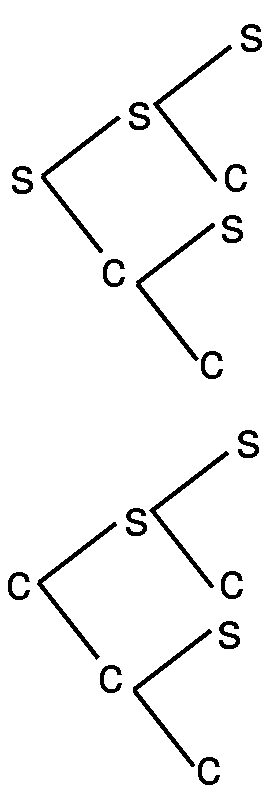
\includegraphics[scale=0.4,bb = 0 0 200 100, draft, type=eps]{/media/antalcides/Antalcides-EXT1/est/bak/est/g11ir300.pdf}\\
 Diagrama de �rbol 
\par\end{center}

\begin{teo}{} Consid�rese un experimento que tiene las dos cara\-cter�sticas
siguientes \end{teo}
\begin{itemize}
\item \textit{El experimento se realiza en dos partes }
\item \textit{La primera parte del experimento tiene }$m$ \textit{resultados
posibles }$x_{1},x_{2},x_{3},\cdots,x_{m}$ \textit{independientemente
del resultado} $x_{i}$ \textit{obtenido la segunda parte del experimento
tiene }$n$\textit{\ resultados posibles }$y_{1},y_{2},y_{3},\cdots,y_{n}$\textit{.}\\
\textit{Cada resultado del espacio muestral S del experimento ser�
por tanto, un par de la forma }$\left(x_{i},y_{j}\right)$\textit{\ es
decir } 
\begin{align*}
S & =\left\{ \left(x_{i},y_{j}\right)|i=1,2,3,\cdots m;j=1,2,3\cdots n\right\} \\
n\left(S\right) & =mn
\end{align*}

\end{itemize}
Este teorema puede generalizarse de la siguiente forma

Si un experimento \ puede realizarse con las siguientes caracter�sticas
\begin{itemize}
\item El experimento se realiza en $k$ partes
\item la primera parte puede realizarse con $n_{1}$ resultados posibles
$x_{11},x_{12},x_{13},\cdots,x_{1n_{1}}$ e independientemente del
resultado $x_{1i}$ se pueden realizar la segunda parte con $n_{2}$
resultados posibles $x_{21},x_{22},x_{23},\cdots,x_{2n_{2}}$ y as�
sucesivamente cada parte del experimento puede realizarse de $n_{l}$
formas, $l=1,2,3,\cdots k$ obteni�ndose un espacio muestral de la
forma 
\begin{align*}
S & =\{(x_{1i},x_{2j},x_{3r},\cdots,x_{km})\}\\
n\left(S\right) & =n_{1}\cdot n_{2}\cdot n_{3}\cdot\cdots\cdot n_{k}
\end{align*}

\end{itemize}
Ahora enunciamos este teorema de una manera diferente.

\begin{teo}{Fundamental}. Si una acci�n puede efectuarse de una de
$p$ maneras diferentes, y si despu�s de que esta acci�n ha sido efectuada
de una de esas maneras, una segunda acci�n puede efectuarse de una
de $q$ maneras diferentes, entonces el n�mero total de maneras diferentes
en que las acciones pueden efectuarse sigui\-endo el orden mencionado
es $pq.$ \end{teo}

\begin{corollary} Si una acci�n puede efectuarse de $p$ maneras
dife\-rentes, y una segunda acci�n puede efectuarse de $q$ maneras
dife\-rentes, y una tercera acci�n puede efectuarse de $r$ maneras
dife\-rentes, y as� sucesivamente, entonces el n�mero total de maneras
diferentes en que pueden realizarse todas estas acciones en el orden
mencionado es $pqr...$ \end{corollary}

\begin{corollary} Si $r$ acciones pueden efectuarse sucesivamente
de $p$ maneras diferentes cada una, entonces el n�mero total de maneras
diferentes en que pueden efectuarse las $r$ acciones sucesivamente
es $p^{r}.$ \end{corollary}


\section{Permutaciones}

\begin{defi}{}{}\index{%
Permutaciones%
}Una permutaci�n es un arreglo de objetos distintos de tal manera que
una permutaci�n difiere de otra si el orden del arreglo o su contenido
difieren \end{defi}

Conviene observar que el orden es una caracter�stica de especial importancia
en una permutaci�n. Cuando cambiamos el orden de los elementos de
este arreglo, se dice que permutamos dichos elementos


\subsection{Muestreo sin reemplazo}

\index{%
Muestreo!Sin reemplazo%
}Consideremos un experimento en el cual se selecciona un objeto de
$n$ objetos distintos, y luego se selecciona un segundo objeto de
los $n-1$ objetos restantes, y as� sucesivamente hasta seleccionar
el �ltimo objeto Este proceso \ se llama muestreo sin reemplazo\ de
acuerdo con el teorema anterior los $n$ objetos se pueden seleccionar
de $n\left(n-1\right)\left(n-2\right)\cdots3\cdot2\cdot1$ $=n!$
formas diferentes\
 Ahora si no se escogen todos los objetos, si no $k$ objetos, los
$k$ objetos se pueden seleccionar 
\begin{align*}
p_{n,k} & =n\left(n-1\right)\left(n-2\right)\cdots\left(n-k+1\right)=\frac{n!}{\left(n-k\right)!}\;\;r\leq n\\
0! & =1\\
1! & =1\\
p_{n,n} & =n\left(n-1\right)\left(n-2\right)\cdots1=n!
\end{align*}


\begin{ejemplo}[] Supongamos que se necesitan dos representantes
del grupo 02 de estad�stica I-ad para asistir a un congreso \end{ejemplo}

\begin{solucion} Como el grupo 02 de estad�stica tiene 40 alumnos
y se necesitan dos, eso quiere decir que que escogen 2 de 40 
\[
p_{40,2}=\frac{40!}{\left(40-2\right)!}=1560
\]


\end{solucion}

\begin{ejemplo}[] Se necesita colocar 7 libros en un estante �De
cuantas formas posibles se pueden colocar? \end{ejemplo}

\begin{solucion} Como se escoger�n 7 de 7 entonces 
\[
p_{7,7}=7!=5040
\]


\end{solucion}


\subsection{Muestreo con reemplazo}

\index{%
Muestreo!Con reemplazo%
}Si suponemos que tenemos una urna con $n$ objetos numerados del $1$
al $n$ y se selecciona un objeto de la urna y se anota su n�mero,
y luego se coloca nuevamente en la urna, luego se selecciona otro
objeto el cual pude ser el primero y as� sucesivamente se pueden seleccionar
tantos objetos como se quieran. Este proceso se denomina muestreo
con reemplazo.

Si queremos realizar un total de $k$ selecciones distintas, se nos
presentan dos posibilidades
\begin{itemize}
\item Si $k>n$, es imposible ya que hay $n$ n�meros posibles y no est�n
repetidos.
\item Si $n\geq k$ Entonces existen $n^{k}$ posibles formas de escoger
los \ $k$ objetos 
\end{itemize}
\begin{ejemplo}[] Si se colocan al azar 12 bolas en 20 urnas, �Cu�l
es la probabilidad de que ninguna urna contenga m�s de una bola \end{ejemplo}

\begin{solucion} Como hay 20 urnas y 12 bolas entonces podemos escoger
12 de 20 posibilidades de colocar las bolas, pero hay 20$^{12}$,
posibles formas de escoger una urna con una bola 
\[
p=\frac{20!}{8!\ast20^{12}}=\frac{235\,702\,467}{16\,\allowbreak000\,000\,000}
\]


\end{solucion}


\paragraph{Coeficiente multinomial}

\index{%
Coeficiente multinomial%
}El n�mero de formas en las que se pueden asignar $n$ objetos distintos
de $k$ grupos diferentes que contienen $n_{1},n_{2},n_{3},\cdots,n_{k}$
objetos respectivamente es 
\begin{align*}
N & =\frac{n!}{n_{1}!n_{2}!n_{3}!\cdots n_{k}!}=\left(\begin{array}{c}
n\\
n_{1}n_{2}n_{3}\cdots n_{k}
\end{array}\right)\\
\text{ donde }n & =\sum_{i=1}^{k}n_{i}
\end{align*}



\subsection{Combinaci�n}

\index{%
Combinaci�n%
}Una combinaci�n es un arreglo de objetos distintos donde una combinaci�n
difiere de otra si difiere el contenido del arreglo. Si nos interesa
determinar el n�mero de combinaciones cuando en $n$ objetos distintos
deben seleccionarse $r$ a la vez entonces 
\[
C_{n,r}=\frac{p_{n,r}}{r!}=\left(\begin{array}{c}
n\\
r
\end{array}\right)\;\;r\leq n
\]
ya que el numerador es el n�mero de permutaciones al escoger $r$
objetos de $n$ posibles, pero hay que descontar los casos en que
el orden determina para la combinaci�n el mismo elemento, que es exactamente
$r!.$


\subsubsection{Propiedades}
\begin{itemize}
\item $\left(\begin{array}{c}
n\\
0
\end{array}\right)=\left(\begin{array}{c}
n\\
n
\end{array}\right)=1$
\item $\left(\begin{array}{c}
n\\
k
\end{array}\right)=\left(\begin{array}{c}
n\\
n-k
\end{array}\right)$
\item $\left(\begin{array}{c}
n\\
k
\end{array}\right)+\left(\begin{array}{c}
n\\
k-1
\end{array}\right)=\left(\begin{array}{c}
n+1\\
k
\end{array}\right)$
\item $C_{n,r}=C_{n-1,r-1}+C_{n-1,r}$
\item El n�mero de maneras en que $mn$ objetos diferentes pueden dividirse
en $m$ grupos de $n$ objetos cada uno, en donde el orden de los
objetos en cada grupo no se toma en consi\-deraci�n, es \\
$\frac{\left(mn\right)!}{\left(n!\right)^{m}},$ considerando el orden
en que se forman los grupos,\\
$\frac{\left(mn\right)!}{\left(n!\right)^{m}m!},$ sin considerar
el orden en que se forman los grupos. 
\end{itemize}
\begin{ejemplo}[] Calcular el n�mero de maneras distintas en que
15 libros diferentes pueden dividirse en tres grupos de 9, 4 y 2 libros
respectivamente.

\begin{solucion} En este caso 
\[
N_{m}=\frac{15!}{9!4!2!}=75075.
\]


\end{solucion} \end{ejemplo}

\begin{ejemplo}[] Se tiene una baraja\footnote{Muchos problemas de probabilidad est�n relacionados con cartas, y
aunque algunos estudiantes est�n relacionados con este juego, lo describiremos
brevemente para que los problemas sean entendidos con claridad. 

Una baraja ordinaria tiene 52 cartas divididas en cuatro grupos o
palos con trece cartas cada uno. Los nombres de los palos y sus colores
son los siguientes: 

Bastos(negros), diamantes(rojos), corazones(rojos) y espadas(negras. 

Cada palo consiste de 9 cartas numeradas del 2 al 10 inclusive y 4
cartas m�s llamadas as, rey, reina y sota (ordenadas en valor descendente).
La expresi�n de que una carta se escoge o saca al azar, significa
que la carta se toma de una baraja bien mezclada del modo que todas
las cartas tengan igual oportunidad de ser escogida.} de 52 cartas diferentes. \end{ejemplo}

Encontrar
\begin{enumerate}
\item El n�mero de maneras en que pueden repartirse las cuatro manos de
13 cartas a cuatro jugadores de bridge
\item El n�mero de maneras en que las 52 cartas pueden dividirse en cuatro
grupos de 13 cartas cada uno. 
\end{enumerate}

\begin{enumerate}
\item En el juego de bridge cada distribuci�n diferente de las manos entre
los jugadores constituye una divisi�n diferente. Por tanto, en este
caso, los grupos aparecen permutados, y por lo tanto, el n�mero de
maneras diferentes es 
\begin{align*}
\frac{52!}{\left(13!\right)^{4}} & =\\
 & 53\,\allowbreak644\,737\,765\,\allowbreak488\,792\,839\,\allowbreak237\,440\,000
\end{align*}

\item En este caso, no importa el orden de los grupos, as� el n�mero de
maneras es 
\begin{align*}
\frac{52!}{\left(13!\right)^{4}4!} & =\\
 & 2235\,197\,406\,\allowbreak895\,366\,368\,\allowbreak301\,560\,000
\end{align*}

\end{enumerate}
\begin{ejemplo}[] Una moneda se tira 10 veces.\ Calcular la probabi\-lidad
de que aparezcan exactamente 7 caras \end{ejemplo}

\begin{solucion} Ya que la moneda tiene dos formas diferentes de
aparecer en cada tiro, en 10 ser�a $2^{10}$ formas. Y de las 10 caras
vamos a seleccionar 7 caras, por lo que ser�an $C_{10,7}$ formas
diferentes, por lo que la probabilidad buscada es 
\[
P=\frac{\binom{10}{7}}{2^{10}}=\frac{15}{128}
\]


\end{solucion}

\begin{ejemplo}[] Si se sacan $3$ cartas al azar de una baraja de
$52$ cartas, calcular la probabilidad de que sean as, rey y reina.
\end{ejemplo}

\begin{solucion} Se pueden seleccionar $3$ cartas al azar entre
$52$, por lo que hay $C_{52,3}\;$formas diferentes. Y como hay $4$palos
y en cada palo hay un as, un rey y una reina, entonces resulta que
estas barajas pueden obtenerse de $4\times4\times4$ formas diferentes
.Por lo que la probabilidad buscada es 
\[
\frac{4^{3}}{\binom{52}{3}}=\frac{16}{5525}=2.\,\allowbreak895\,9\times10^{-3}
\]


\end{solucion}

\begin{ejemplo}[] De una bolsa que que contiene 4 bolas blancas,
2 negras y 3 rojas, se sacan 5 al azar. Calcular la probabilidad de
que 2 sean blancas 1 negra y 2 rojas. \end{ejemplo}

\begin{solucion} Del total de $4+2+3=9$ bolas se pueden seleccionar
5 bolas en $C_{9,5}$ formas diferentes. Ahora entre las 4 bolas blancas
2 de ellas pueden seleccionarse $C_{4,2}$, entre las 2 blancas $C_{2,1}$
y entre las 3 rojas $C_{3,2}$ formas por lo que el total de casos
favorables es $C_{4,2}C_{2,1}C_{3,2}$, as� 
\[
P=\frac{\binom{4}{2}\binom{2}{1}\binom{3}{2}}{\binom{9}{5}}=\frac{2}{7}
\]


\end{solucion}


\section{Probabilidad condicionada e independencia de eventos}

\begin{defi}{}{}\index{%
Probabilidad!condicionada%
}Sean $A,B\in\mathcal{A}$ y sea $B$ un evento de probabilidad no
nula para el evento $A$, llamamos probabilidad condicionada de $A$
a $B$ a la cantidad que representamos $P\left(A|B\right)$ y que
definimos 
\[
P\left(A|B\right)=\frac{P\left(AB\right)}{P\left(B\right)},
\]
la cantidad $P\left(A|B\right)$ se lee la probabilidad de $A$ dada
la ocu\-rrencia de $B$ \end{defi}

\begin{ejemplo}[]\index{%
Eventos!Independencia%
}Se lanza al aire un dado �Cu�l es la probabilidad de que salga el
n�mero 4? si sabemos que el resultado ha sido par \end{ejemplo}

\begin{solucion} Sea $A=\{4\}$, entonces $P\left(A\right)=\frac{1}{6},$\\
$B=\{2,4,6\},$ \ entonces $P\left(B\right)=\frac{3}{6}=\frac{1}{2}$\\
por tanto 
\[
P\left(A|B\right)=\frac{P\left(AB\right)}{P\left(B\right)}=\frac{\frac{1}{6}}{\frac{1}{2}}=\frac{1}{3}
\]


\end{solucion}

\begin{defi}{}{} Sean $A,B\in\mathcal{A}$ dos eventos de probabilidad
no nula se dice que son independientes si y solo si 
\[
P\left(AB\right)=P\left(A\right)P\left(B\right)
\]


\end{defi}

\begin{ejemplo}[] Para cierta poblaci�n de empleados, los porcentajes
de quienes aprueban un examen de aptitud para un trabajo, especificados
seg�n el sexo, se muestran en la tabla. Es decir todas las personas
que presentan el examen el 24\% cae en la categor�a de hombre aprobado,
el 16\% en la categor�a de de hombre reprobado, y as� sucesivamente.
Se selecciona al azar un empleado de esta poblaci�n. Sea $A$ el evento
de que el empleado aprueba el examen y $H$ el evento de que se selecciona
un hombre �Son independientes los eventos $A$ y $H$ ? 
\[
\begin{tabular}{|c|c|}
\hline  &  sexo\\
\hline \begin{tabular}{l}
Resultado\\
 Aprueba \ensuremath{\left(A\right)}\\
 Reprueba\ensuremath{\left(A^{\prime}\right)}\\
 Total 
\end{tabular}  &  \begin{tabular}{lll}
Mujer\ensuremath{\left(M\right)}  &  Hombre\ensuremath{\left(H\right)}  &  Total\\
 24  &  36  &  60\\
 16  &  24  &  40\\
 40  &  60  &  100 
\end{tabular} 
\\\hline \end{tabular}
\]


\begin{solucion} Determinemos 
\begin{align*}
P\left(A|H\right) & =\frac{{}}{{}}\\
 & =\_\_\_\_\_\_\\
 & =\_\_\_\_\_\_\\
 & =\_\_\_\_\_\_\_
\end{align*}


\end{solucion} \end{ejemplo}


\subsection{Reglas multiplicativas}

\index{%
Reglas multiplicativas%
}

\begin{teo}{} Sea $A_{1},A_{2},A_{3},\cdots A_{n}\in\mathcal{A}$
una sucesi�n de eventos aleatorios, entonces 
\[
P\left(\bigcap_{i=1}^{n}A_{i}\right)=P\left(A_{1}\right)P\left(A_{2}|A_{1}\right)P\left(A_{3}|A_{1}A_{2}\right)\cdots P\left(A_{n}|\bigcap_{i=1}^{n-1}A_{i}\right)
\]


\end{teo}

\begin{defi}{}{} Se dice que una colecci�n de eventos independientes
$A_{1},A_{2},A_{3},\cdots A_{n}\in\mathcal{A}$ es un evento exhaustivo
y excluyente de sucesos, si se verifican las siguientes condiciones
\begin{align*}
\bigcup_{i=1}^{n}A_{i} & =S\\
A_{i}\cap A_{j} & =\phi\qquad\forall i\neq j
\end{align*}


\end{defi}
\begin{figure}[ptbh]
\centering{}\includegraphics[scale=0.4]{62_media_antalcides_Antalcides-EXT1_est_bak_est_pdf_Image1.pdf}\caption{%
$A_{1},A_{2},A_{3},A_{4}$ y $A_{5}$ forman un sistema exhaustivo
y excluyente de sucesos%
}
\label{fig 3.5}
\end{figure}


\begin{teo}{} sea $A_{1},A_{2},A_{3},\cdots A_{n}\in\mathcal{A}$
un sistema exhaustivo y excluyente de sucesos. Entonces 
\[
\forall B\subset\mathcal{A},\Longrightarrow P\left(B\right)=\sum_{i=1}^{n}P\left(B|A_{i}\right)P\left(A_{i}\right)
\]


\end{teo}

\begin{figure}[ptbh]
\centering{}\includegraphics[scale=0.4]{63_media_antalcides_Antalcides-EXT1_est_bak_est_pdf_particion.pdf}\caption{%
Si $A_{1},A_{2},A_{3},A_{4}$ forman un sistema exhaustivo y excluyente
de sucesos , podemos calcular la probabilidad de $B$ a partir de
las cantidades $P\left(B\cap A_{i}\right)$%
}
\label{fig 3.6}
\end{figure}


\begin{prueba} Como $B\subset S$ podemos decir 
\begin{align*}
P\left(B\right) & =P\left(B\cap\left(\bigcup_{i=1}^{n}A_{i}\right)\right)\\
 & =P\left(\bigcup_{i=1}^{n}\left(B\cap A_{i}\right)\right)\\
 & =\sum_{i=1}^{n}P\left(B\cap A_{i}\right)\\
 & =\sum_{i=1}^{n}P\left(B|A_{i}\right)P\left(A_{i}\right)
\end{align*}


\begin{ejemplo}[] Se tienen dos urnas, y cada una de ellas contiene
un n�mero diferente de bolas blancas y rojas: \end{ejemplo} \end{prueba}
\begin{itemize}
\item \textit{primera urna }$U_{1}\mathit{:}$ \textit{3 bolas blancas y
2 roja}s
\item \textit{Segunda urna }$U_{2}$\textit{\ 4 bolas blancas y 2 rojas} 
\end{itemize}
\textit{Se realiza el siguiente experimento :}

\textit{Se tira una moneda al aire y si sale cara se elige una bola
de la primera urna y si sale sello se escoge una bola de la segunda
urna.}

\textit{�Cu�l es la probabilidad de que salga una bola blanca?}

\begin{solucion} La situaci�n que tenemos la podemos esquematizar
de la siguiente manera\\
Si $B$: es el evento de sacar una bola blanca y $R$ : el evento
de sacar una bola roja, entonces 
\begin{align*}
P\left(U_{1}\right) & =\frac{1}{2}\\
P\left(B|U_{1}\right) & =\frac{3}{5}\\
P\left(U_{2}\right) & =\frac{1}{2}\\
P\left(B|U_{2}\right) & =\frac{4}{6}
\end{align*}
Como $U_{1}$ y $U_{2}$ forman un sistema exhaustivo y excluyente
de sucesos aplicando el teorema de la probabilidad total podemos afirmar
que, 
\begin{align*}
P\left(B\right) & =P\left(B|U_{1}\right)P\left(U_{1}\right)+P\left(B|U_{2}\right)P\left(U_{2}\right)\\
 & =\frac{3}{5}\cdot\frac{1}{2}+\frac{4}{6}\cdot\frac{1}{2}=\frac{19}{30}
\end{align*}


\end{solucion}

\begin{teo}{} (Bayes) Sea $A_{1},A_{2},A_{3},\cdots A_{n}\in\mathcal{A}$
un sistema exhaustivo y excluyente de eventos. \index{%
Teorema!Bayes%
}Sea $B\subset\mathcal{A}$ un suceso del que conocemos todas las cantidades
\[
P\left(B|A_{i}\right),i=1,2,3,\cdots,n
\]
a las que denominamos verosimilitudes, entones se verifica 
\[
\forall j=1,2,3,\cdots,n,\qquad P\left(A_{j}|B\right)=\frac{P\left(B|A_{j}\right)P\left(A_{j}\right)}{\sum_{i=1}^{n}P\left(B|A_{i}\right)P\left(A_{i}\right)}
\]


\end{teo}\begin{prueba} Es consecuencia de la definici�n de probabilidad
condicionada en t�rminos de la intersecci�n, y del teorema de la probabilidad
total 
\begin{align*}
P\left(A_{j}|B\right) & =\frac{P\left(A_{j}\cap B\right)}{P\left(B\right)}\\
 & =\frac{P\left(B|A_{j}\right)P\left(A_{j}\right)}{\sum_{i=1}^{n}P\left(B|A_{i}\right)P\left(A_{i}\right)}
\end{align*}


\end{prueba}

\begin{ejemplo}[] Se tienen tres urnas. Cada una de ellas contiene
un n�mero diferente de bolas blancas y rojas. La primera urna tiene
3 bolas blancas y 2 rojas, la segunda 4 bolas blancas y 2 rojas y
la tercera 3 bolas rojas.\\
Se realiza el siguiente experimento:\\
Algui�n elije al azar y con la misma probabilidad una de las tres
urnas, saca una bola.\\
Si el resultado del experimento ha sido sacar una bola blanca �Cu�l
es la probabilidad de que provenga de la primera urna? Calcular lo
mismo para las otras dos urnas. \end{ejemplo}

\begin{solucion} Si $B$: es el evento de sacar una bola blanca y
$R$: el evento de sacar una bola roja, entonces como \\
\begin{tabular}{ll}
$U_{1}:$  &
3 bolas blancas y 2 rojas\tabularnewline
$U_{2}:$  &
4 bolas blancas y 2 rojas\tabularnewline
$U_{3}:$  &
3 bolas rojas \tabularnewline
\end{tabular}\\
tenemos 
\begin{align*}
P\left(U_{1}\right) & =\frac{1}{3}\\
P\left(U_{2}\right) & =\frac{1}{3}\\
P\left(U_{3}\right) & =\frac{1}{3}\\
P\left(B|U_{1}\right) & =\frac{3}{5}\\
P\left(B|U_{2}\right) & =\frac{4}{6}\\
P\left(B|U_{3}\right) & =0
\end{align*}
En este caso $U_{1},U_{2},U_{3}$ forman un sistema incompatible y
excluyente de eventos, por lo que es posible aplicar el teorema de
Bayes 
\begin{align*}
P\left(U_{1}|B\right) & =\frac{P\left(B|U_{1}\right)P\left(U_{1}\right)}{P\left(B|U_{1}\right)P\left(U_{1}\right)+P\left(B|U_{2}\right)P\left(U_{2}\right)+P\left(B|U_{3}\right)P\left(U_{3}\right)}\\
 & =\frac{\left(\frac{3}{5}\right)\left(\frac{1}{3}\right)}{\left(\frac{3}{5}\right)\left(\frac{1}{3}\right)+\left(\frac{4}{6}\right)\left(\frac{1}{3}\right)+0\left(\frac{1}{3}\right)}\\
 & =\frac{9}{19}
\end{align*}
\\
Para los otros dos casos resulta de manera equivalente 
\begin{align*}
P\left(U_{2}|B\right) & =\frac{P\left(B|U_{2}\right)P\left(U_{2}\right)}{P\left(B|U_{1}\right)P\left(U_{1}\right)+P\left(B|U_{2}\right)P\left(U_{2}\right)+P\left(B|U_{3}\right)P\left(U_{3}\right)}\\
 & =\frac{10}{19}
\end{align*}
\begin{align*}
P\left(U_{3}|B\right) & =\frac{P\left(B|U_{3}\right)P\left(U_{3}\right)}{P\left(B|U_{1}\right)P\left(U_{1}\right)+P\left(B|U_{2}\right)P\left(U_{2}\right)+P\left(B|U_{3}\right)P\left(U_{3}\right)}\\
 & =0
\end{align*}


\end{solucion}

\begin{ejemplo}[] En la segunda guerra mundial, uno de los primeros
intentos de investigaci�n de operaciones en la Gran Breta�a se orientaba
en establecer patrones de b�squeda de submarinos desde vuelos de escuadrones
o mediante un s�lo avi�n. Por alg�n tiempo, la tendencia fue concentrar
los vuelos en la costa, pues se pensaba que le mayor n�mero de avistamientos
que ocurr�an ah�. El grupo de investigaci�n registr� 1000 vuelos de
un solo avi�n con los sigui\-entes resultados( Los datos no son reales)\\
\\
\begin{tabular}{|l|l|l|l|}
\hline 
 &
En la playa  &
Fuera de la costa  &
Total\tabularnewline
\hline 
Observaci�n  &
80  &
20  &
100\tabularnewline
\hline 
No observaci�n  &
820  &
80  &
900\tabularnewline
\hline 
Total de salidas  &
900  &
100  &
1000\tabularnewline
\hline 
\end{tabular}\\
sea\\
\begin{tabular}{ll}
$S_{1}$  &
Hubo un avistamiento\tabularnewline
$S_{2}$  &
No hubo avistamiento\tabularnewline
$B_{1}$  &
Salida a la costa\tabularnewline
$B_{2}$  &
Salida en altamar \tabularnewline
\end{tabular}\\
Vemos de inmediato que 
\begin{align*}
P\left(S_{1}|B_{1}\right) & =\frac{80}{900}=\frac{4}{45}=8.\,\allowbreak888\,9\times10^{-2}\\
P\left(S_{2}|B_{2}\right) & =\frac{20}{100}=0.\,\allowbreak2
\end{align*}
lo cual indica una estrategia de b�squeda es contraria a la primera
pr�ctica. \end{ejemplo}

\begin{ejemplo}[] Sup�ngase que se va a seleccionar una muestra ale\-atoria
de tama�o 2 de un lotes de tama�o 100, y que se sabe que 98 de los
100 art�culos se encuentran en buen estado. La muestra se toma de
manera tal que el primer art�culo se observa y se regresa antes de
seleccionar el segundo art�culo \end{ejemplo}

\begin{solucion} . Si aceptamos \ que \\
$A$ : El primer art�culo observado est� en buen estado \\
$B$ : El segundo art�culo observado est� en buen estado \\
Y si deseamos determinar la probabilidad de que ambos art�culos est�n
en buen estado, entonces 
\[
P\left(A\cap B\right)=P\left(A\right)P\left(B\right)=\left(\frac{98}{100}\right)\left(\frac{98}{100}\right)=0.\,\allowbreak960\,4
\]
Si se selecciona el art�culo sin reemplazo de modo que que el primer
art�culo no se regresa antes de seleccionar el segundo, entonces 
\[
P\left(A\cap B\right)=P\left(A\right)P\left(B|A\right)=\frac{98}{100}\cdot\frac{97}{99}=0.9602
\]
Los resultados son muy parecidos por lo que generalmente suponemos
que los eventos son independientes cuando la fracci�n de muestreo
(tama�o de la muestra/tama�o de la poblaci�n) es menor que 0.1 \end{solucion}

\begin{ejemplo}[] Tres industrias suministran microprocesadores a
un fabricante de equipos de telemetr�a. Todos se elaboran supuestamente
con las mismas especificaciones. No obstante, el fabricante ha probado
durante varios a�os los microprocesadores, y los re\-gis\-tros indican
la siguiente informaci�n\\
\begin{tabular}{|l|l|l|}
\hline 
Industria  &
Fracci�n de defectos  &
Fracci�n suministrada por\tabularnewline
\hline 
1  &
0.02  &
0.15\tabularnewline
\hline 
2  &
0.01  &
0.80\tabularnewline
\hline 
3  &
0.03  &
0.05\tabularnewline
\hline 
\end{tabular}\\
EL fabricante ha interrumpido las pruebas por causa de los costos
involucrados, y puede ser razonable suponer que la proporci�n defectuosa
y la mezcla de inventarios son las mismas que durante el periodo en
el que se efectuaron los registros. El director de manu\-factura
selecciona un microprocesador al azar, lo lleva al de\-par\-tamento
de pruebas y descubre que est� defectuoso. Determinar la probabilidad
que el art�culo proviene de la industria 3\\
Sea $A$ el evento de que el art�culo es defectuoso y $B_{i}\;i=1,2,3$
es el evento que el art�culo proviene de la empresa $i$ 
\begin{align*}
P\left(B_{3}|A\right) & =\frac{P\left(A|B_{2}\right)P\left(B_{2}\right)}{P\left(A|B_{1}\right)P\left(B_{1}\right)+P\left(A|B_{2}\right)P\left(B_{2}\right)+P\left(A|B_{3}\right)P\left(B_{3}\right)}\\
 & =\frac{\left(0.05\right)\left(0.03\right)}{\left(0.15\right)\left(0.02\right)+\left(0.8\right)\left(0.01\right)+\left(0.05\right)\left(0.03\right)}=0.\,\allowbreak12
\end{align*}


\end{ejemplo}

\begin{ejemplo}[] Una caja contiene 8 bolas rojas, 3 bolas blancas
y nueve azules. Si se sacan 3 bolas al azar, determinar la proba\-bili\-dad
de que \end{ejemplo}
\begin{enumerate}
\item[\foreignlanguage{english}{a.}] \textit{\ Las 3 sea rojas}
\item[\foreignlanguage{english}{b.}] \textit{\ Las tres sean blancas}
\item[\foreignlanguage{english}{c.}] \textit{2 sean rojas}
\item[\foreignlanguage{english}{d.}] \textit{\ Al menos una blanca}
\item[\foreignlanguage{english}{e.}] \textit{\ Sea una de cada color}
\item[\foreignlanguage{english}{f.}] \textit{Salgan en el orden roja,blanca y azul} 
\end{enumerate}
\begin{solucion} \textit{\ Denotaremos por }$R_{i}\;i=1,2,3$\textit{\ los
eventos que la primera, la segunda y la tercera bola sean rojas respectivamente.
Denotaremos por }$B_{i}\;i=1,2,3$ los eventos que la primera, la
segunda y la tercera bola sean blancas respectivamente, y\textit{\ denotaremos
por }$A_{i}\;i=1,2,3$\textit{\ los eventos que la primera, la segunda
y la tercera bola sean rojas respectivamente, entonces} \end{solucion}
\begin{enumerate}
\item[\foreignlanguage{english}{a.}] 
\[
P\left(\bigcap_{i=1}^{3}R_{i}\right)=\frac{\left(\begin{array}{c}
8\\
3
\end{array}\right)}{\left(\begin{array}{c}
20\\
3
\end{array}\right)}=\frac{14}{285}
\]
\end{enumerate}
\begin{description}
\item [{b.}] 
\[
P\left(\bigcap_{i=1}^{3}B_{i}\right)=\frac{\left(\begin{array}{c}
3\\
3
\end{array}\right)}{\left(\begin{array}{c}
20\\
3
\end{array}\right)}=\frac{1}{1140}
\]

\item [{c.}] 
\[
P\left(\bigcap_{i=1}^{2}R_{i}\cap B\right)=\frac{\left(\begin{array}{c}
8\\
2
\end{array}\right)}{\left(\begin{array}{c}
20\\
3
\end{array}\right)}=\frac{\_}{\_}
\]

\item [{d.}] 
\[
P\left(\text{ninguna es blanca}\right)=\frac{\left(\begin{array}{c}
17\\
3
\end{array}\right)}{\left(\begin{array}{c}
20\\
3
\end{array}\right)}=\frac{\_}{\_}
\]

\item [{e.}] 
\[
P\left(\text{sacar una de cada color}\right)=\frac{\left(\begin{array}{c}
8\\
1
\end{array}\right)\left(\begin{array}{c}
3\\
1
\end{array}\right)\left(\begin{array}{c}
9\\
1
\end{array}\right)}{\left(\begin{array}{c}
20\\
3
\end{array}\right)}=\frac{\_}{\_}
\]

\item [{f.}] 
\begin{align*}
 & P\left(\text{bolas en el orden R, B,A}\right)\\
 & =\frac{1}{3!}P\left(\text{una de cada colore}\right)=\frac{3}{95}
\end{align*}

\end{description}
\begin{ejemplo}[] De una baraja de 52 naipes \ bien mezclada se
sacan 5 naipes. Hallar la probabilidad de que 3 sean de un palo y
2 de otro \end{ejemplo}

\begin{solucion}
\begin{align*}
P\left(\text{3 de cualquier figura y 2 de otra}\right) & =\\
 & =\frac{4\binom{13}{3}\cdot3\binom{13}{2}}{\binom{52}{5}}\\
 & =0.\,\allowbreak103
\end{align*}


\end{solucion}

\begin{ejemplo}[] Sup�ngase que se lanzan 12 dados. Se determina
la probabilidad $p$ de que cada uno de los seis n�meros distintos
aparezca dos veces \end{ejemplo}

\begin{solucion} tenemos que $S$ es el conjunto formado por la sucesi�n
de 12-tupla donde la i-�simo valor de la sucesi�n es el resultado
i-�simo lanzamiento, de lo que se deduce que $n\left(S\right)=6^{12}$
donde todos los $6^{12}$ resultados posibles son igualmente probables,
ahora podemos considerar los seis valores posibles que se puede dar
en cada dado como seis casillas las cuales \ se le pueden asignar
solo dos posibilidades. Por lo que al utilizar el coeficiente multinomial
para determinar los casos favorables tenemos 
\begin{align*}
n & =12\\
k & =6\\
n_{1} & =n_{2}=\cdots=n_{6}=2\\
N & =\frac{12!}{\left(2!\right)\left(2!\right)\cdots\left(2!\right)}=\frac{12!}{\left(2!\right)^{6}}
\end{align*}
Por lo que la probabilidad buscada es\\
$P=\frac{12!}{2^{6}6^{12}}$ $=$ $\frac{1925}{559\,872}=$ $3.\,\allowbreak438\,3\times10^{-3}$
\end{solucion}

\begin{ejemplo}[] Una baraja de 52 cartas contiene 13 corazones.
Su\-p�ngase que se barajan las cartas y se distribuyen entre cuatro
jugadores A,B,C y D de tal manera que a cada jugador le corres\-pondan
13 cartas, Se determinar� la probabilidad $P$ de que cada jugador
reciba 6, 4, 2 y 1 \ corazones respectivamente \end{ejemplo}

\begin{solucion} El n�mero de combinaciones distintas posibles de
las 13 posiciones ocupadas en la baraja por los corazones es $\binom{52}{13}$.
Si el jugador A recibe 6 corazones, hay $\binom{13}{6}$ combinaciones
posibles de las 6 posiciones que ocupan estos corazones entre las
13 cartas que recibe el jugador A. De la misma manera podemos establecer
las combinaciones posibles de cada jugador entre las 13 cartas que
recibe cada uno como $\binom{13}{4},\binom{13}{2}$ y $\binom{13}{1}$
respectivamente para B,C y D. Por tanto como los eventos A,B,C y D
son independientes 
\[
P\left(ABCD\right)=\frac{\binom{13}{6}\binom{13}{4}\binom{13}{2}\binom{13}{1}}{\binom{52}{13}}=1.\,\allowbreak9592\times10^{-3}
\]


\end{solucion}

\begin{ejemplo}[] Sup�ngase que una moneda equilibrada va a ser lanzada
diez veces y se desea determinar \end{ejemplo}
\begin{description}
\item [{a.}] \textit{\ la probabilidad }$P$\textit{\ de obtener exactamente
3 caras}
\item [{b.}] \textit{\ La probabilidad }$P$\textit{\ de obtener a lo
sumo tres caras} 
\end{description}
\begin{solucion} \qquad{}\qquad{}\end{solucion}
\begin{enumerate}
\item[\foreignlanguage{english}{a.}] El n�mero total de posibles combinaciones distintas de 10 caras y
sellos es $2^{10}$ y se puede suponer que todas estas combinaciones
son igualmente probables y el n�mero de casos favorables \ es \ $\binom{10}{3}$
por lo que 
\[
p=\frac{\binom{10}{3}}{2^{10}}=0.\,\allowbreak117\,19
\]

\end{enumerate}
\begin{solucion} 
\begin{description}
\item [{b.}] Puesto que lo que me piden es la union de los eventos $A_{i}$
: obte\-ner 0,1,2 y 3 caras \ $i=0,1,2,3$, y como estos eventos
son disjuntos tenemos que 
\[
P\left(\bigcup_{i=0}^{3}A_{i}\right)=\frac{\binom{10}{0}+\binom{10}{1}+\binom{10}{2}+\binom{10}{3}}{2^{10}}=0.\,\allowbreak171\,88
\]

\end{description}
\end{solucion}

\begin{ejemplo}[] Sup�ngase que en una clase hay 15 hombres y 30
mujeres, y que se van a seleccionar al azar 10 estudiantes para una
tarea especial. se determinar� la probabilidad $P$ de seleccionar
exactamente 3 hombres \end{ejemplo}

\begin{solucion} el n�mero de combinaciones distintas que se pu\-eden
formar con 45 estudiantes para obtener una muestra de 10 es $\binom{45}{10},$
y como el muestreo es al azar y sin reemplazo entonces todas estas
combinaciones son igualmente posibles por lo que hay que determinar
el n�meros de combinaciones \ distintas que se pueden seleccionar
con 3 hombres y 7 mujeres, entonces con los hombres se pueden realizar
$\binom{15}{3}$ y con las mujeres $\binom{30}{7}$ por lo que 
\[
P=\frac{\binom{15}{3}\binom{30}{7}}{\binom{45}{10}}=\frac{3958\,500}{13\,633\,279}=0.\,\allowbreak290\,36
\]


\end{solucion}

\begin{ejemplo}[] Sup�ngase que se baraja un naipe de 52 cartas que
contiene 4 ases y que las cartas se reparten entre cuatro jugadores,
de forma que cada una reciba 13 cartas. se determinar� la proba\-bilidad
de que cada jugador reciba un as. \end{ejemplo}

\begin{solucion} El n�mero de combinaciones diferentes es $\binom{52}{4}.$
Y podemos suponer que todas estas combinaciones son igualmente probables.
si cada jugador recibe un as entonces debe haber un as entre las 13
cartas que recibe por ejemplo el primer jugador y un as recibir� cada
uno de los jugadores de las 13 cartas que recibir�n, es decir hay
13 posiciones posibles para el as que recibe cada jugador por lo que
los casos favorables ser� $13^{4},$ entonces 
\[
P=\frac{13^{4}}{\binom{52}{4}}=\frac{2197}{20\,825}=0.\,\allowbreak105\,5
\]


\end{solucion}

\begin{ejemplo}[] Sup�ngase que una m�quina produce un art�culo defectuoso
con probabilidad $p=0.4$ y produce un art�culo no defectuoso con
una probabilidad $q=0,6$. Sup�ngase adem�s que se seleccionan aleatoriamente
para su control seis de los art�culos producidos por la m�quina y
que los resultados de control son independientes para estos seis art�culos.
Se determinar� la probabilidad de que exactamente dos de los seis
art�culos sean defectuosos \end{ejemplo}

\begin{solucion} Si consideramos los eventos $D_{i}$ el evento del
que el $i-\acute{e}simo$ art�culo sea defectuoso y $N_{j}$ el evento
de que el $\ i-\acute{e}simo$ art�culo sea no defectuoso para, $i=1,2,3,4,5,6,$
como los eventos son independientes entonces por ejemplo 
\[
P\left(N_{1}N_{3}D_{2}D_{4}D_{5}D_{6}\right)=qqpppp
\]
como esta es una de las posibles combinaciones hay que determinar
las otras que no es m�s que $\binom{6}{2}$ combinaciones distintas
y por el th 3.13 tenemos 
\[
P=\binom{6}{2}\left(0.4\right)^{2}\left(0.6\right)^{4}=0.\,\allowbreak311\,04
\]


\end{solucion}

\begin{ejemplo}[] consid�rese una m�quina que produce un art�culo
defectuoso con una probabilidad $p=0.4$ y uno no defectuoso con probabilidad
$q=0.6$. Sup�ngase que el control se realiza seleccionando art�culos
al azar y de uno en uno hasta obtener exactamente cinco art�culos
defectuosos. Se determinar� \ la probabilidad $P$ de que deban ser
seleccionados 20 art�culos para obtener 5 defectuosos \end{ejemplo}

\begin{solucion} El quinto art�culo defectuoso ser� el $n-\acute{e}simo$
controlado si, y s�lo si, hay exactamente cuatro defectuosos entre
los primeros $\ n-1$ art�culos y el $n-\acute{e}simo$ es defectuoso
entonces por el th 3.13 tenemos que 
\begin{align*}
P & =\binom{n-1}{4}p^{5}q^{n-5}=\binom{19}{4}\left(0.4\right)^{5}\left(0.6\right)^{15}\\
 & =1.\,\allowbreak866\,2\times10^{-2}
\end{align*}


\end{solucion}

\begin{ejemplo}[] Sup�ngase que se van a extraer dos bolas aleatoriamente
y sin reemplazo, de una urna que contiene 8 bolas rojas y 10 bolas
azules. Se determinar� la probabilidad $P$ de obtener la primera
bola roja y la segunda azul \end{ejemplo}

\begin{solucion} Sea A el evento de que la primera bola sea roja
y B de que la segunda bola sea azul, entonces $P\left(A\right)=\frac{8}{18}=0.\,\allowbreak444\,44$,
adem�s si el suceso A ha ocurrido, entonces se ha obtenido una bola
roja de la urna en la primera extracci�n por lo que la probabilidad
de obtener una bola azul en la segunda extracci�n es 
\[
P\left(B|A\right)=\frac{10}{17}=0.\,\allowbreak588\,24
\]
entonces 
\[
P\left(AB\right)=\left(0.\,\allowbreak444\,44\right)\left(0.\,\allowbreak588\,24\right)=0.\,\allowbreak261\,44
\]


\end{solucion}

\begin{ejemplo}[] Para la fabricaci�n de un gran lote de art�culos
similares se utilizaron tres m�quinas $M_{1},M_{2}$ y $M_{3}$. Sup�ngase
que el 20\% de los art�culos fueron fabricados por la m�quina $M_{1}$,
el 30\% por la m�quina $M_{2}$ y el 50\% por la m�quina $M_{3}$
Suponemos adem�s que el 1\% de los art�culos fabricados por la m�quina
$M_{1}$ son defectuosos y as� respectivamente 2\% y 3\% de los art�culos
fa\-bricados por la m�quinas $M_{2}$ y $M_{3}$. Se quiere seleccionar
al azar uno de los art�culos del lote que resultan defectuosos. Determine
la probabilidad de que el art�culo haya sido fabricado por la m�quina
$M_{2}$. \end{ejemplo}

\begin{solucion} Sea $A_{i}$ el evento de que el art�culo haya sido
fa\-bricado por la m�quina $M_{i},i=1,2,3,$ y sea B el suceso de
que el art�culo seleccionado sea defectuoso, de acuerdo con esto hay
que determinar $P\left(A_{2}|B\right)$, entonces 
\begin{align*}
P\left(A_{1}\right) & =0.2\\
P\left(A_{2}\right) & =0.3\\
P\left(A_{3}\right) & =0.5\\
P\left(B|A_{1}\right) & =0.01\\
P\left(B|A_{2}\right) & =0.02\\
P\left(B|A_{3}\right) & =0.03
\end{align*}
aplicando el teorema de Bayes 
\[
P\left(A_{2}|B\right)=\frac{P\left(A_{2}\right)P\left(B|A_{2}\right)}{\sum_{i=1}^{3}P\left(A_{i}\right)P\left(B|A_{i}\right)}=0.26
\]


\end{solucion}

\problemas{ 
\begin{enumerate}
\item Tres clases diferentes tienen 20, 18 y 25 estudiantes, respectivamente,
y cada estudiante pertenece a una sola clase. Si se forma un equipo
con un estudiante de cada una de estas tres clases, �de cu�ntas maneras
distintas se pueden seleccionar los miembros del equipo?
\item �De cu�ntas maneras distintas se pueden ordenar cinco letras a, b,
c, d y e?
\item Si un hombre tiene seis camisas distintas y cuatro pares distintos
de pantalones, �de cu�ntas formas distintas se puede vestir combinando
esas prendas?
\item Si se lanzan cuatro dados, �cu�l es la probabilidad de que los cuatro
n�meros que aparecen sean distintos?
\item Si se lanzan seis dados, �cu�l es la probabilidad de que cada uno
de los seis n�meros posibles aparezcan exactamente una vez?
\item Si se colocan al azar 12 bolas en 20 urnas, �cu�l es la probabilidad
de que ninguna urna contenga m�s de una bola?
\item El ascensor de un edificio empieza a subir con cinco personas y para
en siete pisos. Si la probabilidad de que cualquier pasajero salga
del ascensor en un piso concreto es igual para todos los pisos y los
pasajeros salen independientemente unos de otros, �cu�l es la probabilidad
de que no haya dos pasajeros que salgan en el mismo piso?
\item Si $k$ personas se sientan aleatoriamente en una fila de $n$ asientos
$(n>k)$, �cu�l es la probabilidad de que ocupen $k$ asientos contiguos
en la fila?
\item Si$k$ personas se sientan aleatoriamente en $n$ sillas dispuestas
en c�rculo $(n>k)$, �cu�l es la probabilidad de que ocupen $k$ sillas
contiguas del c�rculo?
\item Si $n$ personas se sientan aleatoriamente en una fila de $2n$ asientos,
�cu�l es la probabilidad de que no haya dos personas sentadas en asientos
contiguos?
\item Una caja contiene 24 bombillas, de las cuales 2 son defectuosas. S�
una persona selecciona 10 bombillas al azar, sin reemplazo, �cu�l
es la probabilidad de seleccionar las 2 bombillas defectuosas?
\item Sup�ngase que se ha de seleccionar un comit� de 12 personas aleatoriamente
escogidas entre un grupo de 100. Determ�nese la probabilidad de que
dos personas concretas, A y B, sean seleccionadas.
\item Sup�ngase que 35 personas se dividen aleatoriamente en dos equipos
de manera que uno de los equipos consta de 10 personas y el otro de
25. �Cu�l es la probabilidad de que dos personas concretas, A y B,
est�n en el mismo equipo?
\item Una caja contiene 24 bombillas, de las cuales 4 son defectuosas. Si
una persona selecciona aleatoriamente 10 bombillas de la caja, y una
segunda persona toma entonces las 14 bombillas restantes, �cu�l es
la probabilidad de que la misma persona seleccione las 4 bombillas
defectuosas?
\item Demu�strese que, para cualquier entero positivo $n$ y $k$ ($n>k),$
\[
\binom{n}{k}+\binom{n}{k-1}=\binom{n+1}{k}
\]

\item Demu�strese que 
\[
\binom{n}{0}+\binom{n}{1}+\binom{n}{2}+\cdots+\binom{n}{n}=2^{n}
\]

\item El Senado de Estados Unidos est� constituido por dos senado\-res
de cada uno de los 50 estados,

\begin{enumerate}
\item Si se selecciona aleatoriamente un comit� de 8 senadores, �cu�l es
la probabilidad de que contenga al menos uno de los dos senadores
de un estado concreto?
\item �Cu�l es la probabilidad de que un grupo de 50 senadores seleccionados
aleatoriamente contenga un senador de cada estado? 
\end{enumerate}
\item Sup�ngase que$A$ es un suceso tal que $P(A)=0$ y que $B$\ es cualquier
otro suceso. Demu�strese que $A$ y$B$ son sucesos independientes.
\item Sup�ngase que una persona lanza tres veces dos dados equilibrados.
Determ�nese la probabilidad de que en cada uno de los tres lanzamientos
la suma de los dos n�meros que aparecen sea 7.
\item Sup�ngase que la probabilidad de que el sistema de control utilizado
en una nave espacial no funcione en un vuelo concreto es 0.001. Sup�ngase
adem�s que la nave tambi�n tiene instalado un segundo sistema de control
id�ntico, pero completamente independiente del primero, que toma el
control cuando el primero falla. Determ�nese la probabilidad de que
en un vuelo concreto la nave espacial est� bajo control, ya sea del
sistema original o del sistema duplicado.
\item Sup�ngase que una loter�a consta de 10 000 boletos y que otra loter�a
consta de 5000. Si una persona compra 100 boletos de cada loter�a,
�cu�l es la probabilidad de que gane al menos un primer premio?
\item Dos estudiantes A y B est�n inscritos en un curso. Si el estudiante
A asiste a las clases el 80\% de las veces y el estudiante B el 60\%,
y si las ausencias de los dos estudiantes son independientes, �cu�l
es la probabilidad de que al menos uno de los dos estudiantes est�
en clase un d�a concreto?
\item Si se lanzan tres dados equilibrados, �cu�l es la probabilidad de
que los tres n�meros que aparecen sean iguales?
\item Consid�rese un experimento en el cual se lanza una moneda equilibrada
hasta que aparece una cara por primera vez. Si este experimento se
repite tres veces, �cu�l es la probabilidad de que se necesite exactamente
el mismo n�mero de lanzamientos para cada una de las tres repeticiones?
\item Sup�ngase que $A$, $B$ y $C$ son tres sucesos independientes tales
que $P(A)=\frac{1}{4},\;P(B)=\frac{1}{3},\;$y $P(C)=\frac{1}{2}$
.

\begin{enumerate}
\item Determ�nese la probabilidad de que ninguno de estos tres sucesos ocurra
\item Determ�nese la probabilidad de que ocurra exactamente uno de estos
tres sucesos. 
\end{enumerate}
\item Sup�ngase que la probabilidad de que una part�cula emitida por un
material radiactivo penetre en cierto campo es 0.01. Si se emiten
diez part�culas,

\begin{enumerate}
\item �cu�l es la probabilidad de que exactamente una de ellas penetre en
el campo?
\item Si se emiten diez part�culas, �cu�l es la probabilidad de que al menos
una de ellas penetre en el campo?
\item �Cu�ntas part�culas tienen que ser emitidas para que la probabilidad
de que al menos una part�cula penetre en el campo sea al menos 0.8? 
\end{enumerate}
\item En la Serie Mundial de B�isbol, dos equipos A y B juegan una serie
de partidos uno contra otro y el primer equipo que gana un total de
cuatro partidos es el ganador de la Serie Mundial. Si la probabilidad
de que el equipo A gane un partido contra el equipo B es $\frac{1}{3}$,
�cu�l es la probabilidad de que el equipo A gane la Serie Mundial?
\item 15. El Senado de Estados Unidos est� constituido por dos senadores
de cada uno de los 50 estados, (a) Si se selecciona aleatoriamente
un comit� de 8 senadores, �cu�l es la probabilidad de que contenga
al menos uno de los dos senadores de un estado concreto? (b) �Cu�l
es la probabilidad de que un grupo de 50 senadores seleccionados aleatoriamente
contenga un senador de cada estado?
\item La probabilidad de que una persona nade es de 0.45 y la probabilidad
de que una persona cace es de 0.58. Si la probabilidad de que una
persona cace sabiendo que tambi�n caza es 0.21, encuentre la probabilidad
de que:

\begin{enumerate}
\item Cace y nade
\item Cace si tambi�n nada
\item Cace y no nade
\item Cace o nade 
\end{enumerate}
\item La tabla adjunta muestra las frecuencias relativas para el daltonismo
en hombres y mujeres, donde H representa hombres, M mujeres, D dalt�nico
y ND no dalt�nico 
\[
\begin{tabular}{l|ll}
  &  H  &  M\\
\hline D  &  0.042  &  0.007\\
 ND  &  0.485  &  0.466 
\end{tabular}
\]
Si se escoge a una persona al azar, use la tabla para determinar las
probabilidades siguientes:

\begin{enumerate}
\item $P\left(H\right)$
\item $P\left(H\cap D\right)$
\item $P\left(D\right)$
\item $P\left(H\cap ND\right)$ 
\end{enumerate}
\item Si $P\left(E\right)=0.2$ y $P\left(F\right)=0.3.$ Responda si puede
ser cierto en cada una de las preguntas dadas y si es posible plantee
un ejemplo.

\begin{enumerate}
\item �$P\left(E\cup F\right)=0.5?$
\item �$P\left(E\cup F\right)=0.7?$
\item �$P\left(E\cup F\right)=0.4?$
\item �$P\left(E\cap F\right)=0.2?$
\item �$P\left(E\cap F\right)=0.3?$
\item �$P\left(E\cap F\right)=0.1?$
\item �$P\left(E\cap F\right)=0.4?$ 
\end{enumerate}
\item Si cuatro hombres y cuatro mujeres se colocan en fila, �Cu�l es la
probabilidad de que un arreglo aleatorio de los ocho individuos tenga

\begin{enumerate}
\item hombres y mujeres alternados?
\item A los hombres todos juntos? 
\end{enumerate}
\item De un conteo de tarjetas numeradas dei 1 al 10000. �Cu�l es la probabilidad
de que el n�mero que te toque sea divisible exactamente por 5?
\item Un especialista en alergias alega que el 50\% de sus pacientes sufre
de alergia �Cu�l es la probabilidad de que

\begin{enumerate}
\item de que 3 de sus siguientes cuatro pacientes sufran de alergia?
\item Ninguno de los cuatro pacientes sufran de alergias? 
\end{enumerate}
\item De una caja que contiene 6 pelotas negras y 4 verdes, se sacan 3 en
sucesi�n, reemplaz�ndose cada una en la caja antes de extraer la siguiente.
�Cu�l es la probabilidad de que

\begin{enumerate}
\item las 3 sen del mismo color
\item sea al menos una de cada color 
\end{enumerate}
\item Un embarque de 12 televisores contiene 3 defectuosos. �En cuantas
formas puede un hotel comprar 5 y recibir al menos 2 de los defectuosos?
\item En una cierta ciudad, 40\% de los votantes son Liberales y el 60\%
son conservadores; 70\% de los republicanos y el 80\% de los dem�cratas
est�n a favor de una de una consulta popular. al seleccionar al azar
un votante de la ciudad, �Cu�l es la probabilidad de qu� est� a favor
\ de la consulta ?
\item �Cu�ntas manos de bridge que contengan 4 espadas, 6 diamantes, 1 de
bastos y 2 de corazones son posibles?
\item Una empresa industrial grande utiliza 3 hoteles locales para proporcionar
alojamiento a sus clientes durante la noche. De pasadas experiencias
se sabe que al 20\% de ellos se les asigna habitaci�n en \ el hotel
de Santa Marta, el 50\% en Cartagena y al 30\% en Tol�. Si existe
una falla en el servicio de plomer�a en el 5\% de la habitaciones
en Santa Marta , en el 4\% en Cartagena y del 8\% en Tol�. �Cu�l es
la probabilidad de que

\begin{enumerate}
\item a un cliente se le asigne un cuarto con problemas en plomer�a ?
\item a una persona con un problema en plomer�a se asigne el hotel en Cartagena? 
\end{enumerate}
\item Un espacio muestral de 200 adultos se clasifica de acuerdo con su
sexo y nivel de educaci�n 
\[
\begin{tabular}{|l|l|l|}
\hline Educaci�n  &  Hombre  &  Mujer\\
\hline Primaria  &  38  &  45\\
\hline Secundaria  &  28  &  50\\
\hline Bachillerato  &  22  &  17
\\\hline \end{tabular}
\]
Si se selecciona aleatoriamente a una persona de ese grupo, encuentre
la probabilidad de que

\begin{enumerate}
\item no tenga grado de profesional dado de que sea mujer
\item sea hombre dado que tiene educaci�n superior 
\end{enumerate}
\item Se lanzan un par de dados, si se sabe que uno de ellos resulta en
un 4, �cu�l es la probabilidad de que

\begin{enumerate}
\item el otro caiga en 6
\item el total de ambos sea 9 
\end{enumerate}
\item Supongamos que se selecciona al azar un individuo de la pobla\-ci�n
de todos los adultos hombres que en los Estados Unidos. Sea a el evento
en que el individuo seleccionado tenga una estatura de m�s de 6 pies,
y B el evento de que el individuo seleccionado sea un jugador profesional
de baloncesto. �Cu�l considera que sea mayor $P\left(B|A\right)$
o $P\left(A|B\right)?.$ �Por qu�?
\item Un circuito flexible se selecciona al azar de una corrida de producci�n
de 1000 circuitos. Los defectos de manufactura se clasifican en tres
diferentes tipos, denominados A. B y C. Los defectos de tipo A ocurren
el 2 por ciento de las veces, los del tipo B, el 1 por ciento, y los
de tipo C, el 1.5 por ciento. Adem�s, se sabe que el 0.5 por ciento
tienen los defectos de tipo A y B, el 0.6 por ciento, los defectos
B y C, y el 0.4 por ciento presenta los defectos B y C, en tanto que
el 0.2 por ciento tiene los tres defectos. �Cu�l es la probabilidad
de que el circuito flexible seleccionado tenga al menos uno de los
tres tipos de defectos?
\item En un laboratorio de factores humanos, se miden tiempos de reacci�n,
por ejemplo, el tiempo que transcurre desde el instante en que se
despliega un n�mero de posici�n en un tablero digital hasta que el
sujeto presiona un bot�n localizado en la posici�n indicada. Participan
dos sujetos, midi�ndose el tiempo en segundos para cada individuo
$\left(t_{1},t_{2}\right).$ �Cu�l es el espacio muestral para este
experimento? Presente los siguientes eventos como subconjuntos y m�rquelos
sobre un diagrama: 
\[
\left(\frac{t_{1}+t_{2}}{2}\right)\leq0.15,\;\max\left(t_{1},t_{2}\right)\leq0.15,\;\left|t_{1}-t_{2}\right|<0.6.
\]

\item Durante un periodo de 24 horas se entrar� a un procesamiento computarizado.
En un tiempo X y se saldr� en tiempo Y $\geq$ X. Consid�rense X y
Y medido en horas en la linea del tiempo con el inicio del periodo
de 24 horas como el origen. El experimento consiste en observar X
y Y, (X, Y).

\begin{enumerate}
\item Describa el espacio muestral $S$.
\item Dibuje los siguientes eventos en el plano X, Y.

\begin{enumerate}
\item El tiempo de utilizaci�n es una hora o menos
\item El acceso es antes de $t_{1}$ y la salida despu�s de $t_{2}$, donde
$0\leq t_{1}\leq t_{2}\leq24$
\item El tiempo de utilizaci�n es menor que el 20 por ciento del periodo. 
\end{enumerate}
\end{enumerate}
\item Se prueban diodos de un lote uno a la vez y se marcan ya sea como
defectuosos o como no defectuosos. Esto contin�a hasta encontrar dos
art�culos defectuosos o cuando se han probado cinco art�culos. Describa
el espacio muestral para este experimento.
\item Un conjunto tiene cuatro elementos $A=\{a,b,c,d\}$. Describa el conjunto
partes de $A$ .
\item Describa el espacio muestral para cada uno de los siguientes experimentos:

\begin{enumerate}
\item Un lote de 120 tapas de bater�as para celdas de marcapasos contiene
varias defectuosas debido a un problema con el material de barrera
que se aplica en el sistema de alimentaci�n. Se seleccionan tres tapas
al azar (sin reemplazo) y se inspeccionan con cuidado siguiendo una
reducci�n.
\item Una paleta de 10 piezas fundidas contiene una unidad defectuosa y
nueve en buen estado. Se seleccionan cuatro piezas al azar (sin reemplazo)
y se inspeccionan. 
\end{enumerate}
\item El gerente de producci�n de cierta compa��a est� interesado en probar
un producto terminado, que se encuentra disponible en lotes de tama�o
50. A �l le gustar�a volver a elaborar un lote si tiene la completa
seguridad de que el 10 por ciento de los art�culos son defectuosos.
Decide seleccionar una muestra al azar de 10 art�culos sin reemplazo
y volver a producir el lote si �ste contiene uno o m�s art�culos defectuosos.
�Este procedimiento parece razonable?
\item Una firma de transporte tienen un contrato para enviar una carga de
mercanc�as de la ciudad W a la ciudad Z. No hay rutas directas que
enlacen W con Z, pero hay seis carreteras de W a X y cinco de X a
Z. �Cu�ntas rutas en total deben considerarse?
\item Un estado tienen un mill�n de veh�culos registrados y est� considerando
emplear placas de licencia con seis s�mbolos en los que los primeros
tres sean letras y los �ltimos tres, d�gitos. �Es �ste esquema factible?
\item El gerente de una peque�a planta desea determinar el n�mero de maneras
en que puede asignar trabajadores al primer turno. Cuenta con 15 hombres
que pueden servir como operadores del equipo de producci�n, 8 que
pueden desempe�arse como personal de mantenimiento y 4 que pueden
ser supervisores. Si el turno requiere 6 operadores, 2 trabajadores
de mantenimiento, y 1 supervisor, �de cu�ntas maneras puede integrarse
el primer turno?
\item Un lote de producci�n tiene 100 unidades de las cuales 20 se sabe
que est�n defectuosas. Una muestra aleatoria de 4 unidades se selecciona
sin reemplazo. �Cu�l es la probabilidad de que la muestra no contenga
m�s de 2 unidades defectuosas?
\item En la inspecci�n de lotes de mercanc�as que est�n por recibirse, se
emplea la siguiente regla de inspecci�n en lotes que contienen 300
unidades; se selecciona una muestra al azar de 10 art�culos. Si no
hay m�s que un art�culo defectuoso en la muestra, se acepta el lote.
De otro modo se regresa al vendedor. Si la fracci�n defectuosa en
el lote original es $p^{\prime}$, determinar la probabilidad de aceptar
el lote como una funci�n de $p^{\prime}$
\item En una planta de pl�sticos, 12 tubos vac�an diferentes qu�micos en
un tanque de mezcla. Cada tubo tienen una v�lvula de cinco posiciones
que mide el flujo dentro del tanque. Un d�a, mientras se experimenta
con diferentes mezclas, se obtiene una soluci�n que emite un gas venenoso,
no habi�ndose registrado los valores en las v�lvulas. �Cu�l es la
probabilidad de obtener esta misma soluci�n cuando se experimenta
de nuevo de manera aleatoria?
\item Ocho hombres y ocho mujeres con las mismas habilidades solicitan dos
empleos. Debido a que los dos nuevos empleados deben trabajar estrechamente,
sus personalidades deben ser compatibles. Para lograr esto, el administrador
de personal ha aplicado una prueba y debe comparar las calificaciones
para cada posibilidad. �Cu�ntas comparaciones debe efectuar el administrador?
\item En forma casual, un qu�mico combin� dos sustancias de laboratorios
que produjeron un producto conveniente. Desafortunadamente, su asistente
no registr� los nombres de los ingredientes. Hay cuarenta sustancias
disponibles en el laboratorio. Si las dos en cuesti�n deben encontrarse
mediante experimentos sucesivos de ensayo y error, �cu�l es el n�mero
m�ximo de pruebas que pueden realizarse?
\item Un prisionero pol�tico ser� enviado a Siberia o a los Urales. Las
probabilidades de que lo env�en a estos dos lugares son 0.6 y 0.4,
respectivamente. Se sabe adem�s que si un residente de Siberia se
elige al azar hay una probabilidad de 0.5 de que lleve un abrigo de
piel, en tanto que la probabilidad para lo mismos es de 0.7 en el
caso de un residente de los Urales. Al llegar al exilio, la primera
persona que ve el prisionero no lleva un abrigo de piel. �Cu�l es
la probabilidad de que est� en Siberia?
\item Se dise�a un dispositivo de frenado para evitar que un autom�vil patine
en el que incluye un.sistema electr�nico e hidr�\-ulico. El sistema
completo puede descomponerse en tres subsistemas en serie que operan
de manera independiente: un sistema electr�nico, un sistema hidr�ulico
y un accionador mec�nico. En un frenado particular, las confiabilidades
de estas unidades son aproximadamente 0.995, 0.993 y 0.994, respectivamente.
Estime la confiabilidad del sistema.
\item Dos bolas se extraen de una urna que contiene $m$ bolas numeradas
del 1 a $m$. Se conserva la primera bola si tiene el n�mero 1, y
se regresa en caso contrario. �Cu�l es la probabilidad de que la segunda
bola extra�da tenga el n�mero 2?
\item Se eligen dos d�gitos al azar de los d�gitos del 1 al 9 y la selecci�n
es sin reemplazo (el mismo d�gito no puede escogerse en ambas selecciones).
Si la suma de los d�gitos es par, encuentre la probabilidad de que
ambos d�gitos sean impares.
\item En cierta universidad 20 por ciento de los hombre y 1 por ciento de
las mujeres miden m�s de dos metros de altura. Asimismo, 40 por ciento
de los estudiantes son mujeres. Si se selecciona un estudiante al
azar y se observa que mide m�s de dos metros de altura, �Cu�l es la
probabilidad de que sea mujer?
\item En un centro de maquinaria hay cuatro m�quinas autom�ticas que producen
tornillos. Un an�lisis de los registros de inspecci�n anteriores produce
los siguientes datos: 
\[
\begin{tabular}{|l|l|l|}
\hline \begin{tabular}{l}
\\
 M�quina 
\end{tabular}  &  \begin{tabular}{l}
Porcentaje de\\
 \multicolumn{1}{c}{producci�n}
\end{tabular}  &  \begin{tabular}{c}
Porcentaje de\\
 \multicolumn{1}{l}{defectos producidos}
\end{tabular} \\
\hline 1  &  15  &  4\\
\hline 2  &  30  &  3\\
\hline 3  &  20  &  5\\
\hline 4  &  35  &  2
\\\hline \end{tabular}
\]
Las m�quinas 2 y 4 son m�s nuevas y se les ha asignado m�s producci�n
que a las m�quinas 1 y 3. Suponga que la combinaci�n de inventarios
refleja los porcentajes de producci�n indicados.

\begin{enumerate}
\item Si se elige un tornillo al azar del inventario, �cu�l es la probabilidad
de que est� defectuoso?
\item Si se elige un tornillo y se encuentra que est� defectuoso, �cu�l
es la probabilidad de que se haya producido en la m�quina 3? 
\end{enumerate}
\item Sup�ngase que $A\subset B$. Demu�strese que $B^{\prime}\subset A^{\prime}.$
\item Para tres sucesos cualesquiera A, B y C, demu�strese que 
\[
A(B\cup C)=(A\cap B)\cup(A\cap C).
\]

\item Para dos sucesos cualesquiera A y B, demu�strese que 
\[
(A\cup B)^{\prime}=A^{\prime}\cap B^{\prime}\;\text{y}\;(A\cap B)^{\prime}=A^{\prime}\cup B^{\prime}.
\]

\item 4. Para cualquier conjunto de sucesos $A_{i}(i\in I)$, demu�strese
que

\begin{enumerate}
\item $\left(\bigcup_{i\in I}A_{i}\right)^{\prime}=\bigcap_{i\in I}A_{i}^{\prime}$
\item $\left(\bigcap_{i\in I}A_{i}\right)^{\prime}=\bigcup_{i\in I}A_{i}^{\prime}$ 
\end{enumerate}
\item 5. Sup�ngase que se selecciona una carta de una baraja de veinte cartas
que contiene diez cartas rojas numeradas del 1 al 10 y diez cartas
azules numeradas del 1 al 10. Sea A el suceso de seleccionar una carta
con un n�mero par, sea B el suceso de seleccionar una carta azul y
sea C el suceso de seleccionar una carta con un n�mero menor que 5.
Descr�banse el espacio muestral $S$ y cada uno de los siguientes
sucesos en palabras y en subconjuntos de $S$:

\begin{enumerate}
\item $A\cap B\cap C$.
\item $B\cap C^{\prime.}$
\item $A\cup B\cup C.$
\item $A\cap(B\cup C).$
\item $A^{\prime}\cap B^{\prime}\cap C^{\prime}.$ 
\end{enumerate}
\item Un estudiante seleccionado de una clase puede ser chico o chica. Si
la probabilidad de que un chico sea seleccionado es 0.3, �cu�l es
la probabilidad de que sea seleccionada una chica?
\item Se selecciona una bola de una urna que contiene bolas rojas, blancas,
azules, amarillas y verdes. Si la probabilidad de seleccionar una
bola roja es $\frac{1}{5}$ y la de seleccionar una blanca es $\frac{2}{5}$
�cu�l es la probabilidad de seleccionar una bola azul, amarilla o
verde?
\item Si la probabilidad de que un estudiante A suspenda un cierto examen
de estad�stica es 0.5, la probabilidad de que un estudiante B suspenda
el examen es 0.2 y la probabilidad de que ambos estudiantes A y B
suspendan el examen es 0.1,

\begin{enumerate}
\item �cu�l es la probabilidad de que al menos uno de estos dos estudiantes
suspenda el examen?
\item �cu�l es la probabilidad de que ni el estudiante A ni el B suspendan
el examen?
\item �cu�l es la probabilidad de que exactamente uno de los dos estudiantes
suspenda el examen? 
\end{enumerate}
\item Consid�rense dos sucesos $A$y $B$ tales que $P(A)=\frac{1}{3}$
y $P(B)=\frac{1}{2}$. Determ�nese el valor de $P(B\cap A^{\prime})$
para cada una de las siguientes condiciones:

\begin{enumerate}
\item $A$ y $B$ son disjuntos
\item $A\subset B$
\item $P(A\cap B)=\frac{1}{8}$ 
\end{enumerate}
\item Si el 50\% de las familias de cierta ciudad est�n suscritas al peri�dico
matinal, el 65\% de las familias al peri�dico vespertino y el 85\%
al menos a uno de los dos peri�dicos, �\ cu�l es la proporci�n de
familias que est�n suscritas a los dos peri�dicos?
\item Consid�rense dos sucesos $A$ y $B$ con $P(A)=0.4$ y $P(B)=$ $0.7$.
Determ�nense los posibles valores m�ximo y m�nimo de $P(A\cap B)$
y las condiciones en las cuales se consigue cada uno de estos valores.
\item Demu�strese que para dos sucesos $A$ y $B$ cualesquiera, la pro\-babilidad
de que exactamente uno de los dos sucesos ocurra est� dada por la
expresi�n 
\[
P(A)+P(B)-2P(A\cap B).
\]

\item Se selecciona un punto $(x,y)$ del cuadrado $S$ que contiene todos
los puntos $(x,y)$ tales que $0\leq x\leq1$ y $0\leq y\leq1.$ Sup�ngase
que la probabilidad de que el punto seleccionado pertenezca a cualquier
subconjunto espec�fico de $S$ es igual al �rea de ese subconjunto.
Determ�nese la probabilidad de cada uno de los siguientes subconjuntos:

\begin{enumerate}
\item el subconjunto de puntos tales que $(x-\frac{1}{2})^{2}+(y-\frac{1}{2})^{2}>\frac{1}{4}$
\item el subconjunto de puntos tales que $\frac{1}{2}<x+y<\frac{3}{2}$
\item el subconjunto de puntos tales que $y<1-x^{2}$
\item el subconjunto de puntos tales que $x=y.$ 
\end{enumerate}
\item Sea $A_{1},A_{2},A_{3},\cdots$ una serie numerable de eventos y sea
\\
$B_{1},B_{2},B_{3},\cdots$otra serie numerable de eventos tal que
\[
B_{1}=A_{1},\;B_{2}=A_{1}^{\prime}\cap A_{2},\;B_{3}=A_{1}^{\prime}\cap A_{2}^{\prime}\cap A_{3}...
\]
Demu�strese que

\begin{enumerate}
\item $P(\bigcup_{i=1}^{\infty}A_{i})=\sum_{i=1}^{\infty}P\left(B_{i}\right)$
\item $P(\bigcup_{i=1}^{n}A_{i})=\sum_{i=1}^{n}P\left(B_{i}\right)\;$para
$n=1,2,3,...$ 
\end{enumerate}
\item Sea $A_{1},A_{2},A_{3},\cdots A_{n}$ una serie cualquiera de eventos,
demostrar que 
\[
P\left(\bigcup_{i=1}^{n}A_{i}\right)\leq\sum_{i=1}^{n}P\left(A_{i}\right)
\]

\item Sup�ngase que una urna contiene una carta azul y cuatro cartas rojas.
A, B, C y D. Sup�ngase tambi�n que dos de estas cinco cartas se extraen
al azar sin reemplazo

\begin{enumerate}
\item Si se sabe que se ha extra�do la carta A, �cu�l es la probabilidad
de que ambas cartas sean rojas?
\item Si se sabe que se ha extra�do una carta roja, �cu�l es la probabilidad
de que ambas cartas sean rojas? 
\end{enumerate}
\item La probabilidad de que cualquier ni�o de una familia determinada tenga
ojos azules es 1/4, y esta caracter�stica es heredada por cada ni�o
de la familia independientemente de los dem�s. Si hay cinco ni�os
en la familia y se sabe que al menos uno de estos ni�os tiene ojos
azules,

\begin{enumerate}
\item �cu�l es la probabilidad de que al menos tres de los ni�os tengan
ojos azules?
\item Consid�rese la familia de cinco nios

\begin{enumerate}
\item Si se sabe que el ni�o m�s peque�o de la familia tiene los ojos azules,
�cu�l es la probabilidad de que al menos tres de los ni�os tengan
ojos azules?
\item Expl�quese por qu� la respuesta es diferente de la respuesta de la
parte (a) 
\end{enumerate}
\end{enumerate}
\item Consid�rese la siguiente versi�n del juego de dados: El jugador lanza
dos dados. S� la suma en el primer lanzamiento es 7 u 11, el jugador
gana el juego. Si la suma en el primer lanzamiento es 2, 3 � 12, el
jugador pierde. Sin embargo, si la suma en el primer lanzamiento es
4, 5, 6, 8, 9 � 10, entonces se lanzan los dos dados una y otra vez
hasta que la suma sea 7, l�o el valor original. Si el valor original
se obtiene por segunda vez antes de obtener 7 u 11, entonces el jugador
gana. Si se obtiene un total de 7 o de 11 antes de obtener el valor
original por segunda vez, entonces el jugador pierde. Determ�nese
la probabilidad de que el jugador gane este juego.
\item En una ciudad determinada, el 30\% de las personas son conservadores,
el 50\% son liberales y el 20\% son independientes. Los registros
muestran que en unas elecciones concretas, vota\-ron el 65\% de los
conservadores, el 82\% de los liberales y el 50\% de los independientes.
Si se selecciona al azar una persona de la ciudad y se sabe que no
vot� en las elecciones pasadas, �\ cu�l es la probabilidad de que
sea un liberal?
\item Sup�ngase que cuando una m�quina est� correctamente ajustada, el 50\%
de los art�culos que produce son de alta calidad y el otro 50\% son
de calidad media. Sup�ngase, sin embargo, que la m�quina est� mal
ajustada durante el 10\% del tiempo y que, en estas condiciones, el
25\% de los art�culos producidos por ella son de alta calidad y el
75\% de los art�culos son de calidad media.

\begin{enumerate}
\item Sup�ngase que cinco art�culos producidos por la m�quina en un tiempo
determinado son seleccionados al azar e inspeccionados. Si cuatro
de estos art�culos son de alta calidad y uno es de calidad media,
�cu�l es la probabilidad de que la m�quina estuviera correctamente
ajustada durante ese tiempo?
\item Sup�ngase que se selecciona un art�culo adicional, que fue producido
por la m�quina al mismo tiempo que los otros cinco, y resulta ser
de calidad media. �Cu�l es la nueva probabilidad final de que la m�quina
estuviera correctamente ajustada? 
\end{enumerate}
\item Sup�ngase que una caja contiene cinco monedas y que la probabilidad
de obtener cara en un lanzamiento es distinta para cada moneda. Sea
$p_{i}$ la probabilidad de obtener cara al lanzar la $i-\acute{e}sima$
moneda $(i=1,...,5)$ y Sup�ngase que $p_{1}=0$, $p_{1}=\frac{1}{4}$,
$p_{3}=1/2$, $p_{4}=3/4$ y $p_{5}=1$. Si se selecciona una moneda
de la caja al azar y que al lanzarla una vez se obtiene una cara.
�Cu�l es la probabilidad final de que se haya seleccionado la $i-\acute{e}sima$
moneda $(i=1,...,5)$? 
\end{enumerate}
}
\end{document}



\chapter{Variables aleatorias}

\index{Variables Aleatorias}\PartialToc


\section{Introducci�n}

Cuando definimos la probabilidad en el axioma 1 del cap�tulo 3 se
estableci� de la siguiente manera 
\[
\begin{array}{ccc}
P:\mathcal{A} & \rightarrow & [0,1]\subset\rz\\
A\in\mathcal{A} & \mapsto & 1\geq P\left(A\right)\geq0
\end{array}
\]
Tomamos un elemento de $\mathcal{A}$ y le asignamos un n�mero, pero
esta forma de trabajar a veces dificulta la interpretaci�n del concepto
de probabilidad, porque los elementos de $\mathcal{A}$ no son n�meros
si no conjuntos, pero que tal si $\mathcal{A}$\ estuviera formado
no por subconjuntos de $S,$ sino por n�meros, entonces consideremos
el ejemplo de lanzar tres monedas al aire para mostrar como podr�amos
hacer esto.

En este caso el espacio muestral es 
\[
S=\{ccc,ccs,csc,css,scc,scs,ssc,sss\}
\]
ahora si definimos una funci�n, por decir $X$ tal que a cada evento
fundamental le asignamos un n�mero de la siguiente forma

\begin{center}
\includegraphics[scale=0.4]{51_home_antalcides_Escritorio_est_libros-est_pdf_Variab.pdf} 
\par\end{center}

De este modo aparece el concepto de variable unidimensional 
\[
\begin{array}{ccc}
X:S & \longrightarrow & \rz\\
e & \longmapsto & X\left(e\right)=x
\end{array}
\]


de acuerdo con el ejemplo anterior se define la variable 
\[
X\equiv n\acute{u}mero\quad de\quad caras
\]
de la siguiente forma 
\begin{align*}
X & :\longrightarrow\rz\\
X\left(CCC\right) & =3\\
X\left(CCS\right) & =X\left(CSC\right)=X\left(SCC\right)=2\\
X\left(CSS\right) & =X\left(SSC\right)=X\left(SCS\right)=1\\
X\left(SSS\right) & =0
\end{align*}
la variable $X$ no recibe el calificativo de aleatoria por el echo
de asignarle a un elemento $e\in S$ un valor num�rico, (por que de
echo este valor esta definido de forma precisa), sino por el echo
de que al realizar el experimento no sabemos que elemento de $S$
puede ocurrir

En funci�n del espacio del rango $R_{X}$ esta funci�n puede ser clasificada
como 
\begin{itemize}
\item Variable aleatoria discreta .\index{Variable!Aleatoria!Discreta}
Si toma un n�mero finito o numerable de valores, por ejemplo 
\[
X:\longrightarrow\nz
\]

\item Variable aleatoria continua.\index{Variable!Aleatoria!continua} Si
toma un n�mero de valores no numerables, por ejemplo 
\[
X:\longrightarrow\rz
\]

\end{itemize}
\begin{defi}{}{} Si $E$ es un experimento que tiene como espacio
muestral a $S$, y $X$ es una funci�n que le asigna un n�mero real
$X\left(e\right)$ a todo resultado $e\in S$, entonces $X$ se llama
variable aleatoria \end{defi} 
\begin{figure}[ptb]
\centering{}\includegraphics[scale=0.4]{52_home_antalcides_Escritorio_est_libros-est_pdf_va2.pdf}\label{fig 4.3} 
\end{figure}


\begin{defi}{}{} Si $S$ es el espacio muestral de un experimento
$E$ y una variable aleatoria $X$ con rango el espacio $R_{X}$ se
define en $S$, y adem�s si el $A\subset S$ y $B\subset R_{X}$,
entonces $A$ y $B$ son eventos equivalentes si 
\begin{align*}
P_{X}\left(B\right) & =P\left(A\right)\\
donde\quad A & =\{e\in S:X\left(e\right)\in B\}
\end{align*}
\par \end{defi}

como indica la \ref{fig 4.4}.

\begin{defi}{}{} Si $A$ $\subset S$ y $B\subset R_{X}$ definimos
la probabilidad de $B$ como 
\[
P_{X}=P\left(X^{-1}\left(B\right)\right)=P\left(A\right)
\]
donde 
\begin{align*}
A & =\{e\in S:X\left(e\right)\in B\}\\
X^{-1}(B) & =\{e\in S:X\left(e\right)\in B\}
\end{align*}
\par \end{defi} 
\begin{figure}[ptb]
\centering{}\includegraphics[scale=0.4]{53_home_antalcides_Escritorio_est_libros-est_pdf_ee.pdf}\label{fig 4} 
\end{figure}


\begin{apunte} si sobre los elementos de $S$ existe una distribuci�n
de probabilidad, esta se transmite a los valores que toma la variable
$X$. Es decir toda variable aleatoria conserva la estructura probabi\-l�stica
del experimento aleatorio que describe, es decir si $P$ es la funci�n
de probabilidad definida sobre $S\in$ $\mathcal{A}$, esta induce
otra funci�n $P_{X}$ definida sobre $\rz$, de forma que conserva
los valores de las probabilidades 
\begin{align*}
P_{X}\left(X=x\right) & =P\left(\{e\in S:X\left(e\right)=x\}\right)\\
P_{X}\left(X\in\left(a,b\right)\right) & =P\left(\{e\in S:X\left(e\right)\in\left(a,b\right)\}\right)
\end{align*}
como indica la \ref{fig 4.4} \end{apunte}

\begin{center}
\includegraphics[scale=0.4]{54_home_antalcides_Escritorio_est_libros-est_pdf_probabilidad.pdf}\\
 Espacio probabil�stico \label{fig 4.4} 
\par\end{center}

De ahora en adelante denotaremos $P_{X}$ como $P$ pero no se debe
confundir con la probabilidad $P$ que definimos en el capitulo 3


\section{Variables aleatorias discretas}

\index{Variables aleatorias!Discretas}

\begin{defi}{}{} Si $X$ es una variable aleatoria discreta, asociamos
un n�mero 
\[
f\left(x_{i}\right)=P\left(X=x_{i}\right)
\]
como cada resultado $x_{i}$ en $R_{X}$ para $i=1,2,3\cdots,n,\cdots,$
donde los n�meros $f\left(x_{i}\right)$ satisfacen \begin{enumerate} 

\item $f\left(x_{i}\right)\geq0\quad$para toda $i$ 

\item $\sum_{i=1}^{x}f\left(x_{i}\right)=1$\index{Funci�n de!Probabilidad}La
funci�n $f\left(x_{i}\right)$ se llama funci�n de probabilidad o
ley de probabilidad de la variable aleatoria, y la colecci�n de pares
$\left(x_{i},f\left(x_{i}\right)\right)$ se llama distribuci�n de
probabilidad de $X$ 

\item Dada una variable aleatoria discreta $X:S\longrightarrow\nz$,
su funci�n de probabilidad $f$ se define de modo que $f\left(x_{i}\right)$
es la proba\-bilidad de que $X$ tome ese valor 
\[
\begin{array}{ccc}
f:\nz & \longrightarrow & [0,1]\\
x_{i} & \longmapsto & f\left(x_{i}\right)=P\left(X=x_{i}\right)
\end{array}
\]
si $x_{i}$ no es uno de los valores que puede tomar $X$, entonces
$f\left(x_{i}\right)=0$ \end{enumerate} \end{defi}

\begin{defi}{}{} {[}Funci�n de distribuci�n{]}De una variable alea\-toria
discreta, $F$ que se define de modo que si $x_{i}\in\rz,F\left(x_{i}\right)$
es igual a la probabilidad de que $X$ tome un valor inferior o igual
a $x_{i}$, es decir, 
\[
\begin{array}{ccc}
F:\nz & \longrightarrow & [0,1]\\
x_{i} & \longmapsto & F\left(x_{i}\right)=P\left(x_{i}\geq X\right)
\end{array}
\]
\par \end{defi}

\begin{apunte} La funci�n de distribuci�n $F$, es una funci�n no
decreciente, es decir. Si 
\[
x_{1<}x_{2}\Longrightarrow F\left(x_{2}\right)\geq F\left(x_{1}\right)
\]
Adem�s, es continua a la derecha 
\[
\lim_{x\longrightarrow a^{+}}F\left(x\right)=F\left(a\right)
\]
y 
\begin{align*}
F\left(-\infty\right) & =\lim_{x\longrightarrow-\infty}F\left(x_{i}\right)=0\\
F\left(+\infty\right) & =\lim_{x\longrightarrow+\infty}F\left(x_{i}\right)=1
\end{align*}
\par \end{apunte}

\begin{ejemplo}{[}{]} Analicemos el experimento del lanzamiento de
la mo\-ne\-da tratado en la introducci�n y determinemos $f\left(x\right),F\left(x\right)$
\[
\begin{tabular}{l}
 Presentaci�n tabular\\
\hline  \multicolumn{1}{|l|}{\ensuremath{\;\;\;\;\;\;\begin{array}{c}
x\\
0\\
1\\
2\\
3
\end{array}\begin{array}{c}
f\left(x\right)\\
1/8\\
3/8\\
3/8\\
1/8
\end{array}}} 
\\\hline \end{tabular}
\]
\\
\par \begin{center} \includegraphics[scale=0.4]{55_home_antalcides_Escritorio_est_libros-est_pdf_GK4FC800.pdf}\\
 Funci�n de probabilidad \par \end{center}\par \begin{center}
\includegraphics[scale=0.4]{56_home_antalcides_Escritorio_est_libros-est_pdf_GK4FD001.pdf}\\
 Funci�n de distribuci�n \par \end{center}\par \end{ejemplo}

\begin{ejemplo}{[}{]} Sup�ngase que tenemos una variable aleatoria
$X$ con una distribuci�n de probabilidad dada por la relaci�n 
\[
f\left(x\right)=\left\{ \begin{array}{cc}
\binom{n}{x}p^{x}\left(1-p\right)^{n-x} & x=0,1,2,...,n\\
0 & \text{de otro modo}
\end{array}\right.
\]
donde $n$ es un entero positivo y $0\leq p\leq1.$ El ejemplo anterior
es un caso particular de �sta distribuci�n de probabilidad llamada
Binomial \end{ejemplo}

\begin{ejemplo}{[}{]} Sup�ngase que hay 100 art�culos de los cuales
hay 5 defectuosos. Se toma una muestra de de 4 art�culos sin reemplazo
Determine la distribuci�n de probabilidad para los art�culos defectuosos
\end{ejemplo}

\begin{solucion} Si $X$ representa el n�mero de art�culos defectuosos
entonces la probabilidad de que se escojan $x$ art�culos defectuosos
es 
\[
f\left(x\right)=P\left(X=x\right)=\frac{\binom{5}{x}\binom{100-5}{4-x}}{\binom{100}{4}}\text{ si }x=0,1,2,3,4
\]
Ya que los casos posibles ser�an $\binom{100}{4}$ porque de 100 se
escogen 4 y los casos favorables ser�a$\ \binom{5}{x}\binom{100-5}{4-x},$
debido a que es una muestra sin reemplazo el n�mero de combinaciones
distintas que se pueden formar con $x$ art�culos defectuosos para
formar una muestra de 5 es $\binom{5}{x}$ y la afirmaci�n de que
se van a escoger 5 al azar significa que todas las $\binom{100-5}{4-x}$
son igualmente posibles \end{solucion} 
\[
\begin{array}{cc}
x & f\left(x\right)\\
0 & 0.805\\
1 & 0.178\\
2 & 0.014\\
3 & 0.003\\
4 & 0.00
\end{array}
\]

\begin{quotation}
{%
\parbox[b]{3.1358in}{%
\begin{center}
\includegraphics[scale=0.4]{57_home_antalcides_Escritorio_est_libros-est_pdf_GK4FJD02.pdf}\\
 Funci�n de probabilidad ej 4.3 
\par\end{center}%
}} 
\end{quotation}
\begin{ejemplo}{[}{]} Sup�ngase que una variable aleatoria $X$ tiene
una distribuci�n discreta con la siguiente funci�n de probabilidad
\[
f\left(x\right)=\left\{ \begin{array}{ccc}
cx & \text{para} & x=1,2,3,4,5\\
0 & \text{en otro caso}
\end{array}\right.
\]
Determine el valor de la constante c\par \begin{solucion} Debido
a que f(x) es una funci�n de probabilidad entonces 
\begin{align*}
\sum_{i=1}^{5}f\left(x_{i}\right) & =1\Longrightarrow\\
15c & =1\Longrightarrow\\
c & =\frac{1}{15}
\end{align*}
\par \end{solucion} \end{ejemplo}

\begin{apunte} Si la variable $X$ puede tomar un n�mero enumerable
de valores $x_{1},x_{2},x_{3},\cdots,$ entoces se tiene que 
\[
\sum_{i=1}^{\infty}f\left(x_{i}\right)=\sum_{i=1}^{\infty}P\left(X=x_{i}\right)=1
\]
\par \end{apunte}


\section{Variables aleatorias continuas}

\index{Variables aleatorias!Continuas}

Cuando tenemos una variable\ aleatoria continua no tiene sentido
realizar una suma de las probabilidades de cada uno de los valores
que toma, ya que el conjunto es no enumerable por lo que hay que introducir
otro concepto.

Sea $f:\rz\longrightarrow\rz$ una funci�n llamada funci�n de\index{Funci�n!De densidad}
densidad de una variable aleatoria continua, integrable que cumple
las propieda\-des 
\begin{align*}
f\left(x\right) & \geq0\\
\int_{-\infty}^{+\infty}f\left(x\right)dx & =1
\end{align*}
adem�s para todo $[a,b]$ se tiene 
\[
P\left(a\leq x\leq b\right)=\int_{a}^{b}f\left(x\right)dx
\]


\begin{center}
\includegraphics[scale=0.4]{58_home_antalcides_Escritorio_est_libros-est_pdf_img813.pdf}\\
 Funci�n de densidad de $f\left(x\right)$\label{fig 4.5} 
\par\end{center}

\begin{apunte} Al observar la \ref{fig 4.5} observamos que $P\left(a\leq x\leq b\right)$
es el �rea bajo la curva de $f$ \end{apunte}

\begin{apunte} Por ser $f$ integrable entonces la la probabilidad
en un punto es nula, es decir 
\[
P\left(X=a\right)=P\left(a\leq x\leq a\right)=\int_{a}^{a}f\left(x\right)dx=0
\]
\par \end{apunte}

\begin{apunte} Debido a lo anterior se tiene que \begin{itemize} 

\item La funci�n de densidad no es �nica 

\item $P\left(a\leq x\leq b\right)=P\left(a<x<b\right)$ 

\item $P\left(a\leq x\leq b\right)=P\left(a\leq x<b\right)=P\left(a<x\leq b\right)$
\end{itemize} \end{apunte}

La funci�n de distribuci�n de una variable aleatoria, $F,$ continua
se define de modo que dado $x\epsilon$ $\rz$, $F\left(x\right)$
es la probabilidad de que $X$ sea mayor o igual que $x,$ es decir
\[
\begin{array}{ccc}
F:\rz & \longrightarrow & [0,1]\\
x & \longmapsto & F\left(x\right)=P\left(x\geq X\right)=\int_{-\infty}^{x}f\left(t\right)dt
\end{array}
\]


\begin{figure}[ptb]
\centering{}\includegraphics[scale=0.4]{59_home_antalcides_Escritorio_est_libros-est_pdf_Img817.pdf}\caption{Funci�n de distribuci�n $F$}
\end{figure}


\begin{proposicion}{} Dado un intervalo de la forma $(a,b]$, tenemos
\begin{align*}
P\left(X\in(a,b]\right) & =\int_{a}^{b}f\left(x\right)dx\\
 & =\int_{-\infty}^{b}f\left(x\right)dx-\int_{-\infty}^{a}f\left(x\right)dx\\
 & =F\left(b\right)-F\left(a\right)
\end{align*}
Se puede observar que la cantidad $F\left(b\right)-F\left(a\right)$
representa la masa de probabilidad extendida alo largo del intervalo
$(a,b]$ . Si dividimos esta cantidad por la longitud del intervalo,
\[
\frac{F\left(b\right)-F\left(a\right)}{b-a}
\]
tenemos la masa media de probabilidad por unidad de longitud en $(a,b]$,
es decir, su densidad media de probabilidad, ahora si 
\[
\lim_{a\longrightarrow b}\frac{F\left(b\right)-F\left(a\right)}{b-a}=F^{\prime}\left(b\right)=f\left(b\right)
\]
que es la densidad de probabilidad en el punto $b$ \end{proposicion}

\begin{apunte} \begin{itemize} 

\item Si $X$ es una variable continua la funci�n de distribuci�n
$F$ es no decreciente, es decir si 
\[
x_{1}<x_{2}\Longrightarrow F\left(x_{2}\right)\geq F\left(x_{1}\right)
\]
\par 

\item esta funci�n es absolutamente convergente y se verifica 
\begin{align*}
F\left(-\infty\right) & =\lim_{x\longrightarrow-\infty}F\left(x\right)=0\\
F\left(+\infty\right) & =\lim_{x\longrightarrow+\infty}F\left(x\right)\left(1\right)
\end{align*}
\par \end{itemize} \end{apunte}

\begin{ejemplo}{[}{]} Suponga que la f.d.p de una variable aleatoria
$X$ es 
\[
f\left(x\right)=\left\{ \begin{array}{ccc}
0 & si & x\leq0\\
\frac{1}{\left(1+x\right)^{2}} & si & x>0
\end{array}\right.
\]
\par \begin{itemize} 

\item Represente graficamente la f.d.p 

\item encuentre la f.d y representela gr�ficamente \end{itemize}
\end{ejemplo}

\begin{solucion} \begin{itemize} 

\item Su representaci�n gr�fica es 
\[
f\left(x\right)=\left\{ \begin{array}{ccc}
0 & si & x\leq0\\
\frac{1}{\left(1+x\right)^{2}} & si & x>0
\end{array}\right.
\]
{%
\parbox[b]{3in}{%
\begin{center}
\includegraphics[scale=0.4]{60_home_antalcides_Escritorio_est_libros-est_pdf_FS31VK01.pdf}\\
 Gr�fica del ejemplo 
\par\end{center}%
}}

\item Si $x>0$ entonces $F\left(x\right)=\int_{0}^{x}\frac{1}{\left(1+t\right)^{2}}dt=\allowbreak1-\frac{1}{1+x}$
entonces 
\[
F\left(x\right)=\left\{ \begin{array}{ccc}
0 & si & x\leq0\\
1-\frac{1}{1+x} & si & x>0
\end{array}\right.
\]
{\includegraphics[scale=0.4]{61_home_antalcides_Escritorio_est_libros-est_pdf_FS331W05.pdf}}
\end{itemize} \end{solucion}

\begin{ejemplo}{[}{]} \begin{itemize} 

\item Determine la\ gr�fica de la f.d.p y determinar la f.d 
\[
f\left(x\right)=\left\{ \begin{array}{ccc}
\frac{4}{3}\left(1-x^{3}\right) & si & 0<x<1\\
0 & si & x\geq1\\
0 & si & 0\leq x
\end{array}\right.
\]
\parbox[b]{3in}{%
\begin{center}
\includegraphics[scale=0.4]{62_home_antalcides_Escritorio_est_libros-est_pdf_FS32PM03.pdf}\\
 f.d.p de $\frac{4}{3}(1-x^{3})$ 
\par\end{center}%
} 

\item Si $0<x<1$ entonces 
\begin{align*}
F\left(x\right) & =1-\int_{x}^{1}\frac{4}{3}\left(1-t^{3}\right)dt=1-\left(\frac{4}{3}x-\frac{1}{3}x^{4}\right)\\
F\left(x\right) & =\left\{ \begin{array}{ccc}
0 & si & x\leq0\\
\frac{4}{3}x-\frac{1}{3}x^{4} & si & 0<x<1\\
1 & si & x\geq1
\end{array}\right.
\end{align*}
\parbox[b]{3in}{%
\begin{center}
\includegraphics[scale=0.5]{63_home_antalcides_Escritorio_est_libros-est_pdf_FS441N02.pdf}\\
 f.d del ejemplo 4.6 
\par\end{center}%
} \end{itemize} \end{ejemplo}


\section{Distribuciones de probabilidad conjuntas}

\index{Distribuciones de probailidad}\index{Distribuciones de probabilidad!Conjuntas}

En muchas situaciones tratamos problemas donde intervienen m�s de
una variable aleatoria en forma simult�nea, por lo que el objetivo
de esta secci�n es el de tratar y formular las distribuciones de probabilidad
conjuntas para dos o m�s variables aleatorias.

\begin{defi}{}{} si $S$ es el espacio muestral de un experimento
$E$, y $X_{1},X_{2},X_{3},\cdots,X_{k}$ son funciones, cada una
de las cuales asignan un n�mero real, $X_{1}\left(x\right),X_{2}\left(x\right),X_{3}\left(x\right),\cdots,X_{k}\left(x\right)$
a cada resultado $x$, designaremos como $\left(X_{1},X_{2},X_{3},\cdots,X_{k}\right)$
el vector $k-dimensional$, el espacio del rango del vector $\left(X_{1},X_{2},X_{3},\cdots,X_{k}\right)$
es el conjunto de todos los valores posibles del vector aleatorio
\end{defi} 
\begin{figure}[ptb]
\centering{}\includegraphics[scale=0.4]{64_home_antalcides_Escritorio_est_libros-est_pdf_vector.pdf}\caption{vector k-dimensional}
\end{figure}


En la mayor parte de esta secci�n trataremos el caso bidimensional
es decir el vector $k-dimensional$ es $\left(X_{1},X_{2}\right)$

\begin{defi}{}{} Funciones de probabilidad bivariada \begin{enumerate} 

\item Caso discreto: para cada resultado $\left(x_{1i},x_{2j}\right)$
de $\left(X_{1},X_{2}\right),$ asociamos un n�mero 
\[
f\left(x_{1i},x_{2j}\right)=P\left(X_{1}=x_{1i},X_{2}=x_{2j}\right)
\]
donde 
\begin{align*}
f\left(x_{1i},x_{2j}\right) & \geq0\text{ }\\
\text{para todo }i & \in I,j\in J\text{ siendo }I,J\text{ conjuntos de sub�ndices}
\end{align*}
y 
\[
\sum_{i\in I}\sum_{j\in J}f\left(x_{1i},x_{2j}\right)=1
\]
Los valores $\left(\left(x_{1i},x_{2j}\right),f\left(x_{1i},x_{2j}\right)\right)$
para todo $i\in I$ y $j\in J$ forman la distribuci�n de probabilidad
de $\left(X_{1},X_{2}\right)$ 

\item Caso continuo . Si $\left(X_{1},X_{2}\right)$ es un vector
aleatorio continuo con espacio del rango, $R,$ en $\rz^{2}$, entonces
$f$, la funci�n de densidad conjunta, tiene las siguientes propiedades
\[
f\left(x_{1},x_{2}\right)\geq0\text{ }\forall\left(x_{1},x_{2}\right)\in R
\]
y 
\[
\int\int_{R}f\left(x_{1},x_{2}\right)dx_{1}dx_{2}=1
\]
\par \end{enumerate} \end{defi}

\begin{defi}{}{} Se dice que $\ n$ variables aleatorias \\
 $X_{1},X_{2},X_{3},\cdots,X_{k},$tiene una distribuci�n discreta
conjunta si el vector aleatorio\\
 $X=\left(X_{1},X_{2},X_{3},\cdots,X_{k}\right)$ puede tomar solamente
un n�mero finito o una sucesi�n finita de valores distintos posibles$\left(x_{1},x_{2},x_{3},\cdots,x_{k}\right)$
en $\rz^{k}$. La funci�n de probabilidad conjunta \ de $X_{1},X_{2},X_{3},\cdots,X_{k}$
se define entonces como la funci�n $f$ tal que para cualquier punto
$x=\left(x_{1},x_{2},x_{3},\cdots,x_{k}\right)\in A\subset$\rz$^{k},$
\[
f\left(x\right)=P\left(X=x\right)\quad\forall x\in A
\]
donde $A$ es cualquier subconjunto de $\rz^{k}$ 
\[
P\left(x\in A\right)=\sum_{x\in A}f\left(x\right)
\]
\par \end{defi}

\begin{defi}{}{} Distribuciones continuas. se dice que $n$ variables
aleatorias $X_{1},X_{2},X_{3},\cdots,X_{k}$ tienen una distribuci�n
conjunta continua si existe una funci�n no negativa $f$ definida
sobre $\rz^{k}$ tal que para cualquier subconjunto $A\subset\rz^{k}$
\begin{align*}
 & P\left(\left(X_{1},X_{2},X_{3},\cdots,X_{k}\right)\in A\right)\\
 & =\int\cdots\int_{A}f\left(x_{1},x_{2},x_{3},\cdots,x_{k}\right)dx_{1}dx_{2}\cdots dx_{k}
\end{align*}
\par \end{defi}

\begin{defi}{}{} La f.d conjunta de $k$ variables aleatorias\\
 $X_{1},X_{2},X_{3},\cdots,X_{k},$ se define como la funci�n $F$
cuyo valor en cualquier punto $\left(x_{1},x_{2},x_{3},\cdots,x_{k}\right)$
de un espacio $k$-dimensional \rz $^{k}$ est� dado por la relaci�n
\[
F\left(x_{1},x_{2},x_{3},\cdots,x_{k}\right)=P\left(X_{1}\leq x_{1},\cdots X_{k}\leq x_{k}\right)
\]
\par \end{defi}

\begin{apunte} �sta f.d satisface todas las propiedades de la f.d
univariada. \end{apunte}

En el caso bivariado. Si $X$ y $Y$ son variables aleatorias con
f.d.p conjunta $f$ se tiene que 
\[
F\left(x,y\right)=\int_{-\infty}^{x}\int_{-\infty}^{y}f\left(u,v\right)dudv
\]


Si la distribuci�n conjunta de $X_{1},X_{2},X_{3},\cdots,X_{k}$ es
continua, entonces la f.d.p conjunta $f$ se puede obtener a partir
de la f.d conjunta $F$ utilizando la relaci�n 
\[
f\left(x_{1},x_{2},x_{3},\cdots,x_{k}\right)=\frac{\partial^{k}F\left(x_{1},x_{2},x_{3},\cdots,x_{k}\right)}{\partial x_{1}\partial x_{2}\cdots\partial x_{k}}
\]
para todos los puntos $\left(x_{1},x_{2},x_{3},\cdots,x_{k}\right)$
donde exista la derivada.

En el caso bivariado 
\[
f\left(x,y\right)=\frac{\partial^{2}F\left(x,y\right)}{\partial x\partial y}
\]
$\forall\left(x,y\right)$ donde exista la derivada parcial de $2$${^{o}}$
orden

\begin{ejemplo}{[}{]} Sup�ngase que la variable aleatoria $X$ puede
tomar solamente los valores 1,2,3, y que la variable $Y$ puede tomar
solamente los valores 1,2,3,4, donde la f.p conjunta de $X$ e $Y$
es como indica la tabla\\
 %
\begin{tabular}{|c|c|c|c|c|}
\hline 
$X|Y$  &
1  &
2  &
3  &
4\tabularnewline
\hline 
1  &
0.1  &
0  &
0.1  &
0\tabularnewline
\hline 
2  &
0.3  &
0  &
0.1  &
0.2\tabularnewline
\hline 
3  &
0  &
0.2  &
0  &
0\tabularnewline
\hline 
\end{tabular}\\
 determine los valores de $P\left(X\geq2,Y\geq2\right)$ y $P\left(X=1\right)$\par \begin{solucion}
Sumando$f\left(x,y\right)$ sobre todos los valores de $x\geq2$ y
de $y\geq2,$ se obtiene 
\begin{align*}
p\left(X\geq2,Y\geq2\right) & =f\left(2,2\right)+f\left(2,3\right)+f\left(2,4\right)+\\
 & +f\left(3,2\right)+f\left(3,3\right)+f\left(3,4\right)\\
 & =0.5\\
P\left(X=1\right) & =\sum_{y=1}^{4}f\left(1,y\right)=0.2
\end{align*}
\par \end{solucion} \end{ejemplo}

\begin{center}
\begin{figure}[ptb]
\centering{}\includegraphics[scale=0.4]{65_home_antalcides_Escritorio_est_libros-est_pdf_Fdp.pdf}\caption{f.d.p del ejemplo 4.7}
\end{figure}

\par\end{center}

\begin{ejemplo}{[}{]} Sup�ngase que la f.d.p conjunta de $X$ e $Y$
es la sigui\-ente 
\[
f\left(x,y\right)=\left\{ \begin{array}{ccc}
cx^{2}y & para & x^{2}\leq y\leq1\\
0 &  & \text{en otro caso}
\end{array}\right.
\]
\par \begin{itemize} 

\item Determine el valor de la constante $c$ 

\item $P\left(X\geq Y\right)$ \end{itemize} \begin{solucion} Sea
el conjunto $S$ de puntos $\left(x,y\right)$ para los que f$\left(x,y\right)>0$
est� representado en la figura 4.8 . puesto que $f\left(x,y\right)=0$
fuera de $S$, resulta que 
\[
\int\int_{s}f\left(x,y\right)dxdy=\int_{-1}^{1}\int_{x^{2}}^{1}cx^{2}ydydx=\frac{4}{21}c
\]
y como esta integral debe ser 1, entonces c=$\frac{21}{4}$\\
 {%
\parbox[b]{2.9706in}{%
\begin{center}
\includegraphics[scale=0.4]{66_home_antalcides_Escritorio_est_libros-est_pdf_imagen4.pdf}
\par\end{center}%
}} \begin{itemize} 

\item Sea $S$$_{0}$ el conjunto donde $x$$\geq y$, entonces 
\begin{align*}
\int\int_{S_{0}}f\left(x,y\right)dxdy & =\\
\int_{0}^{1}\int_{x^{2}}^{x}\frac{21}{4}x^{2}ydydx & =\frac{3}{20}
\end{align*}
\par \begin{center} \includegraphics[scale=0.4]{67_home_antalcides_Escritorio_est_libros-est_pdf_Imagen47.pdf}\\
 Fig(b) Ejemplo 4.8 \label{fig 4.8b} \par \end{center}\par \end{itemize}
\end{solucion} \end{ejemplo}

\begin{ejemplo}{[}{]} Sup�ngase que $X$ e $Y$ son variables aleatorias
que solamente pueden tomar valores en los intervalos \ $0\leq X\leq2,0\leq Y\leq2$.
Sup�ngase tambi�n que la f.d. conjunta de $X$ e $Y$, para todos
los valores $0\leq x\leq2,0\leq y\leq2,$ es la siguiente 
\begin{equation}
F\left(x,y\right)=\frac{1}{16}xy\left(x+2\right)\label{*}
\end{equation}
\par \end{ejemplo}

\begin{solucion} Se determinar� primero la $F$$_{x}$ de la variable
aleatoria $X$ y luego la f.d.p conjunta f de $X$ e $Y$.\\
 El valor de $F\left(x,y\right)$ en cualquier punto $\left(x,y\right)$
del plano $xy$ que nos representa un par de valores posibles de $X$
e $Y$ se puede calcular a partir \ref{*}, teniendo en cuenta que
$F\left(x,y\right)=P\left(X\leq x,Y\leq y\right).$ Por tanto, si
$\ x<0$ o $y<0$, entonces $F\left(x,y\right)=0$. Si $x>2$ o$\ y>2$,
entonces $F\left(x,y\right)=1,$ Si $0\leq x\leq2,y\geq2$ entonces
$F\left(x,y\right)=F\left(x,2\right)$ y resulta de la ecuaci�n \ref{*}
ya que $F\left(x,y\right)=0$ si $y>0$ 
\[
F\left(x,y\right)=\frac{1}{8}x\left(x+2\right)
\]
an�logamente, si $0\leq y\leq2,x>2,$ entonces 
\[
F\left(x,y\right)=\frac{1}{8}y\left(y+2\right)
\]
La funci�n $F$$\left(x,y\right)$ queda as� definida para todo punto
del plano $xy$ .\\
 Haciendo $y\longrightarrow\infty,$ se determina que la f.d de la
variable aleatoria $X$ es 
\[
F_{x}=\left\{ \begin{array}{ccc}
0 & si & x<0\\
\frac{1}{8}x\left(x+2\right) & si & 2\geq x\geq0\\
1 & si & x>2
\end{array}\right.
\]
Adem�s, para $0<x<2,0<y<2,$ 
\[
\frac{\partial^{2}F\left(x,y\right)}{\partial x\partial y}=\frac{1}{8}\left(x+y\right)
\]
Mientras que si $x<0,y<0,x>2,y>2,entonces$ 
\[
\frac{\partial^{2}F\left(x,y\right)}{\partial x\partial y}=0
\]
Por tanto, la f.d.p conjunta de $X$ e $Y$ es 
\[
f\left(x,y\right)=\left\{ \begin{array}{ccc}
\frac{1}{8}\left(x+y\right) & si & 0<x<2,0<y<2\\
0 &  & \text{ en otro caso}
\end{array}\right.
\]
\par \end{solucion}


\subsection{Distribuciones marginales}

\index{Distribuciones!Marginales}

cuando nos interesa conocer la distribuci�n por ejemplo de $X_{1}$
sola\-mente entonces es necesario introducir el concepto de una distribuci�n
lla\-mada marginal 
\begin{itemize}
\item En el caso discreto\ la distribuci�n marginal para $X_{1}$ y $X_{2}$
es 
\begin{align*}
f\left(x_{1}\right) & =\sum_{todo\,j}f\left(x_{1i},x_{2j}\right)\,\forall i=1,2,\cdots\\
f\left(x_{2}\right) & =\sum_{todo\,i}f\left(x_{1i},x_{2j}\right)\,\forall j=1,2,\cdots
\end{align*}

\item En el caso continuo la distribuci�n marginal para $X_{1}$ y $X_{2}$
es 
\begin{align*}
f\left(x_{1}\right) & =\int_{-\infty}^{\infty}f\left(x_{1},x_{2}\right)dx_{2}\\
f\left(x_{2}\right) & =\int_{-\infty}^{\infty}f\left(x_{1},x_{2}\right)dx_{1}
\end{align*}

\end{itemize}

\subsubsection{Tablas de doble entrada}

Consideremos una poblaci�n de $n$ individuos, desde un punto de vista
descriptivo, donde cada uno de ellos presenta dos caracteres que representaremos
mediante las variables $X$ e $Y$ donde la variable $X$ tiene $k$
modalidades y la variable $Y$ tiene $p$ modalidades, el problema
ahora es tratar de representar toda la informaci�n de manera adecuada
y f�cil de interpretar, por lo que creamos una tabla formada por $kp$
celdas de forma que tenga $k$ filas y $p$ columnas, donde la celda
que denotaremos con el sub�ndice $ij$ representar� el n�mero de elementos
de la muestra que presentan simult�neamente las modalidades $x_{i},y_{j}$\\
 $_{\begin{tabular}{|l|l|l|l|l|l|l|l|}
\hline  \ensuremath{X|Y}  &  \ensuremath{y_{1}}  &  \ensuremath{y_{2}}  &  \ensuremath{\cdots}  &  \ensuremath{y_{j}}  &  \ensuremath{\cdots}  &  \ensuremath{y_{p}}  &  total\\
\hline  \ensuremath{x_{1}}  &  n\ensuremath{_{11}}  &  n\ensuremath{_{12}}  &  \ensuremath{\cdots}  &  n\ensuremath{_{1j}}  &  \ensuremath{\cdots}  &  n\ensuremath{_{1p}}  &  n\ensuremath{_{1\cdot}}\\
\hline  \ensuremath{x_{2}}  &  n\ensuremath{_{21}}  &  n\ensuremath{_{22}}  &  \ensuremath{\cdots}  &  n\ensuremath{_{2j}}  &  \ensuremath{\cdots}  &  n\ensuremath{_{2p}}  &  n\ensuremath{_{2\cdot}}\\
\hline  \ensuremath{\vdots}  &  \ensuremath{\vdots}  &  \ensuremath{\vdots}  &  \ensuremath{\ddots}  &  \ensuremath{\vdots}  &  \ensuremath{\ddots}  &  \ensuremath{\vdots}  &  \ensuremath{\vdots}\\
\hline  \ensuremath{x_{i}}  &  n\ensuremath{_{i1}}  &  n\ensuremath{_{i2}}  &  n\ensuremath{_{11}}  &  n\ensuremath{_{ij}}  &  \ensuremath{\cdots}  &  n\ensuremath{_{ip}}  &  n\ensuremath{_{i\cdot}}\\
\hline  \ensuremath{\vdots}  &  \ensuremath{\vdots}  &  \ensuremath{\vdots}  &  \ensuremath{\ddots}  &  \ensuremath{\vdots}  &  \ensuremath{\ddots}  &  \ensuremath{\vdots}  &  \ensuremath{\vdots}\\
\hline  \ensuremath{x_{k}}  &  n\ensuremath{_{k1}}  &  n\ensuremath{_{k2}}  &  \ensuremath{\cdots}  &  n\ensuremath{_{kj}}  &  \ensuremath{\cdots}  &  n\ensuremath{_{kp}}  &  n\ensuremath{_{k\cdot}}\\
\hline  total  &  n\ensuremath{_{\cdot1}}  &  n\ensuremath{_{\cdot2}}  &  \ensuremath{\cdots}  &  n\ensuremath{_{\cdot j}}  &  \ensuremath{\cdots}  &  n\ensuremath{_{\cdot p}}  &  n\ensuremath{_{\cdot\cdot}} 
\\\hline \end{tabular}}$ \\
 El n�mero de individuos que presentan la modalidad $x_{i}$es la
frecuencia absoluta marginal de $x_{i}$ y se representa $n_{i\cdot}$
y evidentemente es 
\[
n_{i\cdot}=\sum_{j=1}^{p}n_{ij}
\]
de manera an�loga se define la frecuencia absoluta marginal para la
modalidad $y_{j}$ 
\[
n_{\cdot j}=\sum_{i=1}^{k}n_{ij}
\]
El n�mero total de elementos es 
\[
n=n_{\cdot\cdot}=\sum_{i=1}^{k}n_{i\cdot}=\sum_{j=1}^{p}n_{\cdot j}
\]
Llamaremos frecuencia relativa $f_{ij}=\frac{n_{ij}}{n}$

las frecuencia relativas marginales ser�an 
\begin{align*}
f_{i\cdot} & =\sum_{j=1}^{p}f_{ij}=\frac{n_{i\cdot}}{n}\\
f_{\cdot j} & =\sum_{j=1}^{p}f_{ij}=\frac{n_{\cdot j}}{n}\\
f_{\cdot\cdot} & =1
\end{align*}


\begin{ejemplo}{[}{]} Sup�ngase que $X$ e Y tienen la f.p conjunta
dada por la tabla del ejemplo 4.7. La f.p marginal $f$$_{x}$ de
$X$ se puede determinar sumando los valores de cada fila de esta
tabla . De esta manera se obtiene que 
\begin{align*}
f_{x}\left(1\right) & =0.2\\
f_{x}\left(2\right) & =0.6\\
f_{x}\left(3\right) & =0.2\\
f_{x}\left(x\right) & =0\text{ para los restantes valores de }x
\end{align*}
\par \end{ejemplo}

\begin{ejemplo}{[}{]} Sup�ngase que la f.p.d conjunta de $X$ e $Y$
es la des\-crita en el ejemplo 4.8. Obtenga la f.d.p marginal\par \begin{solucion}
Se puede observar en la figura (a) del ej. 4.8 que $X$ no puede tomar
ning�n valor fuera del intervalo $-1\leq X\leq1$ Por tanto, $f_{x}\left(x\right)=0$
para $x<-1$ o $x>1.$ Adem�s, para $-1\leq x\leq1$, se observa en
la misma figura que $f\left(x,y\right)=0,$ a menos que $x^{2}\leq y\leq1$.Por
tanto, para $-1\leq x\leq1$ 
\begin{align*}
f_{x}\left(x\right) & =\int_{-\infty}^{\infty}f\left(x,y\right)dy=\\
\int_{x^{2}}^{1}\left(\frac{21}{4}\right)x^{2}ydy & =\frac{21}{8}x^{2}\left(1-x\right)\left(1+x\right)\left(x^{2}+1\right)
\end{align*}
Se puede observar en la figura (a) del ej. 4.8 que Y no puede tomar
ning�n valor fuera del intervalo $0\leq Y\leq1.$ Por tanto, $f_{y}\left(y\right)=0$
para $y<0$ o $y>1$. Adem�s, para $\ 0\leq y\leq1$, se observa en
la misma fig. Que $-\sqrt{y}\leq x\leq\sqrt{y}.$Por tanto, para $0\leq y\leq1$
\begin{align*}
f_{y}\left(y\right) & =\int_{-\infty}^{\infty}f\left(x,y\right)dx=\\
 & =\int_{-\sqrt{y}}^{\sqrt{y}}\left(\frac{21}{4}\right)x^{2}ydx=\left(\frac{7}{2}\right)y^{5/2}
\end{align*}
\par \end{solucion} \end{ejemplo} 


\subsubsection{Variables aleatorias independientes}

Se dice \ que dos variables aleatorias son independientes si Para
$A,B\subset\rz$ 
\[
P(X\in A,Y\in B)=P\left(X\in A\right)P\left(Y\in B\right)
\]
Es decir si 
\begin{align*}
P\left(x\geq X,y\geq Y\right) & =P\left(x\geq X\right)P\left(y\geq Y\right)\\
F\left(x,y\right) & =F_{x}\left(x\right)F_{y}\left(y\right)\\
f\left(x,y\right) & =f_{x}\left(x\right)f_{y}\left(y\right)
\end{align*}
En el caso discreto la independencia nos indicar�a que $X,Y$ son
independientes si 
\[
f_{ij}=f_{i\cdot}\cdot f_{\cdot j}
\]
pero cada una de las relaciones siguientes expresa por si sola la
independencia 
\[
\frac{n_{ij}}{n_{i\cdot}}=\frac{n_{\cdot j}}{n_{\cdot\cdot}}=\frac{n_{2j}}{n_{2\cdot}}=\cdots=\frac{n_{kj}}{n_{k\cdot}}
\]


\begin{ejemplo}{[}{]} Sup�ngase que se toman dos medidas independientes
X eY de lluvia durante un periodo de tiempo en una localidad y que
la f.d.p g de cada medida es la siguiente 
\[
g\left(x\right)=\left\{ \begin{array}{ccc}
2x & si & 0\leq x\leq1\\
0 &  & \text{ en otro caso}
\end{array}\right.
\]
Se determinar� el valor de $P\left(X+Y\leq1\right)$\par \begin{solucion}
Puesto que $X$ e $Y$ son independientes y cada una tiene la f.d.p.
$g$, resulta que para cualquier par de valores $x$ e $y$ la f.d.p.
conjunta $f$$\left(x,y\right)$ de $X$ e $Y$ est� dada por la relaci�n
$f\left(x,y\right)=g\left(x\right)g\left(y\right).$ Por tanto 
\[
f\left(x,y\right)=\left\{ \begin{array}{ccc}
4xy & si & 0\leq x\leq1,0\leq y\leq1\\
0 &  & \text{ en otro caso}
\end{array}\right.
\]
El conjunto $S$ del plano $xy$ en el que $f\left(x,y\right)>0$
y el subconjunto $S$$_{0}$ en el que $x+y\leq1$ se encuentra representado
en la figura 4.9. Por tanto 
\[
P\left(X+Y\leq1\right)=\int_{0}^{1}\int_{0}^{1-x}4xydydx=\frac{1}{6}
\]
\raisebox{-0cm}{%
\parbox[b]{8.8568cm}{%
\begin{center}
\includegraphics[scale=0.4]{68_home_antalcides_Escritorio_est_libros-est_pdf_Image4.pdf}
\par\end{center}%
}} \end{solucion} \end{ejemplo} 


\subsection{Distribuciones discretas}

\index{Distribuciones!Discretas}


\subsubsection{Distribuciones condicionales discretas}

\index{Distribuciones!Condicionales!Discretas}

Sean $X$ e $Y$ dos variables aleatorias que tienen distribuci�n
discreta conjunta cuya f.p. conjunta es $f$, definimos $f_{x},f_{y}$
como las f.p marginales de$\ X$ e $Y$, respectivamente. Si observamos
un valor $y$ de la variable $Y$, la probabilidad de que la variable
aleatoria $X$ tome cualquier valor particular $x$, est� dado por
la siguiente probabilidad condicional 
\begin{align*}
P\left(X=x|Y=y\right) & =\frac{P\left(X=x,Y=y\right)}{P\left(Y=y\right)}\\
 & =\frac{f\left(x,y\right)}{f_{y}\left(y\right)}
\end{align*}
A esta distribuci�n se le denomina distribuci�n condicional de $X$
dado $Y$ y se denota 
\[
f\left(x|y\right)=\left\{ \begin{array}{ccc}
\frac{f\left(x,y\right)}{f_{y}\left(y\right)} & si & f_{y}\left(y\right)>0\end{array}\right.
\]
An�logamente se define la distribuci�n de probabilidad condicional
de $Y$ dado $X$ 
\[
f\left(y|x\right)=\left\{ \begin{array}{ccc}
\frac{f\left(x,y\right)}{f_{x}\left(x\right)} & si & f_{x}\left(x\right)>0\end{array}\right.
\]
La funci�n de densidad conjunta se define 
\begin{align*}
F\left(x|y\right) & =P\left(x\geq X,Y=y\right)\\
 & \text{ para un valor fijo de }y\\
F\left(y|x\right) & =P\left(y\geq Y,X=x\right)\\
 & \text{ Para un valor fijo de }x
\end{align*}


\begin{ejemplo}{[}{]} Analice la independencia para los datos tabulados
\begin{tabular}{|l|l|l|l|l|}
\hline 
$X|Y$  &
$1\in(0,2]$  &
$3\in(2,4]$  &
$5\in(4,6]$  &
$total$\tabularnewline
\hline 
$0$  &
$24$  &
$4$  &
$8$  &
$36$\tabularnewline
\hline 
$1$  &
$6$  &
$1$  &
$2$  &
$9$\tabularnewline
\hline 
$2$  &
$12$  &
$2$  &
$4$  &
$18$\tabularnewline
\hline 
$total$  &
$42$  &
$7$  &
$14$  &
$63$\tabularnewline
\hline 
\end{tabular}\par \end{ejemplo} 


\subsubsection{Distribuciones condicionales continuas}

Sean $X,Y$ variables aleatorias continuas con densidad conjunta $f\left(x,y\right)$
y las densidades marginales $f_{x}\left(x\right),f_{y}\left(y\right)$,
respectrivamente . Entonces la densidad condicional de $X$ dado un
$Y=y$ fijo 
\[
f\left(x|y\right)=\left\{ \begin{array}{ccc}
\frac{f\left(x,y\right)}{fy\left(y\right)} & si & f_{y}\left(y\right)>0\\
0 & en & otro\,caso
\end{array}\right.
\]
De manera an�loga 
\[
f\left(y|x\right)=\left\{ \begin{array}{ccc}
\frac{f\left(x,y\right)}{f_{x}\left(x\right)} & si & f_{x}\left(x\right)>0\\
0 & en & otro\,caso
\end{array}\right.
\]


\begin{ejemplo}{[}{]} Sup�ngase que la f.p conjunta de $X$ e $Y$
es la dada por la tabla del ejemplo 4.7 . Se determinar� la f.p condicional
de Y dado $X=2$\par \begin{solucion} A partir de de la tabla $f$$_{x}\left(x\right)=0.6$.
Por tanto la proba\-bilidad condicional f$\left(y|x\right)=\frac{f\left(2,y\right)}{0.6}$
\ Por ejemplo si $Y=1$ entonces f$\left(1|2\right)=0.5$ \end{solucion}
\end{ejemplo}

\begin{ejemplo}{[}{]} Sea la f.d.p conjunta de X e Y la del ejemplo
4.8 Determinar la f.d.p condicional de Y dado $X=x$ \end{ejemplo}

\begin{solucion} El conjunto $S$ para el cual $f$$\left(x,y\right)>0$
se observa en la figura (a) del ejemplo 4.8 . Adem�s la f.d.p marginal
se obtuvo en el ejemplo 4.11 y se representa en la fig 4.14 .Se puede
observar a partir de esta figura que $f$$_{x}\left(x\right)>0$ para
$-1<x<1$, pero no para $x=0$. Por tanto, para cualquier valor concreto
de $x$ tal que $-1<x<0$ � $0<x<1$, la f.d.p condicional f$\left(y|x\right)$
de Y es la siguiente\par \includegraphics[scale=0.4]{69_home_antalcides_Escritorio_est_libros-est_pdf_FTLPMV02.pdf}\\
 Fig 4.14\par 
\[
f\left(y|x\right)=\left\{ \begin{array}{ccc}
\frac{2y}{1-x^{4}} & si & x^{2}\leq y\leq1\\
0 &  & y>1
\end{array}\right.
\]
En particular si X=0.5 entonces 
\begin{align*}
 & P\left(Y\geq0.75|X=0.5\right)\\
 & =^{\int_{0.75}^{1}{\huge f}\left(y|0.5\right){\huge dy}}=\frac{7}{15}
\end{align*}
\par \end{solucion} 


\subsection{Cambio de variable}

\index{Cambio de variable}


\subsubsection{Funciones de una variable con una distribuci�n discreta}

Sea $X$ una variable aleatoria que tiene una f.p discreta $f$, y
sea $Y=h\left(X\right)$ otra variable aleatoria definida como funci�n
de $X,$ y sea $g$ la f.p discreta de $Y,$ entonces $g$ se puede
obtener a partir de $f$ para cualquier valor $y$ de $Y,$ as� 
\begin{align*}
g\left(y\right) & =P\left(Y=y\right)=\\
P\left(h\left(X\right)=y\right) & =\sum_{\{x:h\left(x\right)=y\}}f\left(x\right)
\end{align*}



\subsubsection{Funciones de una variable con una distribuci�n continua}

Sea $X$ una variable aleatoria que tiene distribuci�n continua, con
una f.d.p de $X$ $f$, se define para otra variable aleatoria $Y=h\left(X\right)$
y para cualquier real $y$, la f.d $G\left(y\right)$ de $Y$ as�
\begin{align*}
G\left(y\right) & =P\left(y\geq Y\right)\\
P\left(y\geq h\left(X\right)\right) & =\int_{\{x:y=h\left(x\right)\}}f\left(x\right)dx
\end{align*}
adem�s si la variable $Y$ tiene una distribuci�n continua, su f.d.p
se puede obtener 
\[
g\left(y\right)=\frac{dG\left(y\right)}{dy}
\]


Lo anterior lo podemos formalizar de la siguiente manera

\begin{proposicion}{} Sea $X$ una variable aleatoria cualquiera.
Si re\-alizamos el cambio de variable $Y=h\left(X\right)$, tenemos
una nueva variable aleatoria de modo que su f.d.p es f y P$\left(a<x<b\right)=1$
y adem�s sup�ngase que $r$$\left(x\right)$ es continua y estrictamente
creciente o estrictamente decreciente en $a<X<b$ si y s�lo si $\alpha<Y<\beta$
y sea $X=h^{-1}\left(Y\right)$ la funci�n inversa de $h$ para $\alpha<Y<\beta,$
entonces la f.d.p de $g$ est� dada por la relaci�n\ 
\[
g\left(y\right)=\left\{ \begin{array}{ccc}
g\left(y\right)=f\left(h^{-1}\left(y\right)\right)\left|\frac{dx}{dy}\right| & si & \alpha<Y<\beta\\
0 &  & \text{en otro caso}
\end{array}\right.
\]
donde se tiene que 
\[
\frac{dx}{dy}=\frac{1}{h^{\prime}\left(h^{-1}\left(y\right)\right)}
\]
En el caso que la aplicaci�n no sea inyectiva, podemos tener para
un $y$ dado ciertos $x_{1},x_{2},x_{3},\cdots,x_{n}$ tales que $f\left(x_{i}\right)=y$
En este caso 
\[
g\left(y\right)=\sum_{i=1}^{n}f\left(x_{i}\right)\left|\frac{dx_{i}}{dy}\right|
\]
\par \end{proposicion}

donde 
\[
\frac{dx_{i}}{dy}=\frac{1}{h^{\prime}\left(x_{i}\right)}
\]


\begin{ejemplo}{[}{]} Sea $X$ una variable aleatoria continua tal
que $Y=X^{2}$en este caso $h\left(x\right)=x^{2}$ la cual no inyectiva
pero si la restringimos a los reales positivos \ y los reales negativos
tenemos que 
\[
g\left(y\right)=f\left(\sqrt{y}\right)\frac{1}{2\sqrt{y}}+f\left(-\sqrt{y}\right)\frac{1}{2\sqrt{y}}
\]
\par \end{ejemplo}

\begin{ejemplo}{[}{]} Sup�ngase que $X$ tiene una distribuci�n f
uniforme sobre el intervalo $\left(-1,1\right)$, as� que 
\[
f\left(x\right)=\left\{ \begin{array}{ccc}
0.5 & si & -1<x<1\\
0 & si & x\geq1,-1\geq x
\end{array}\right.
\]
\par \begin{center} \includegraphics[scale=0.4]{70_home_antalcides_Escritorio_est_libros-est_pdf_FTIYA300.pdf}\\
 Distribuci�n uniforme \par \end{center}\par Determine la f.d.p
para la variable $Y=X$$^{2}$ \end{ejemplo}

\begin{solucion} Como $Y=X$$^{2}$ entonces Y debe pertenecer a
$[0,1]$, entonces para todo y $\in\,\left(0,1\right)$ la f.d G$\left(y\right)$
de $Y$ es 
\begin{align*}
G\left(y\right) & =P\left(y\geq Y\right)\\
P\left(y\geq X^{2}\right) & =P\left(-y^{0.5}\leq X\leq y^{0.5}\right)=\\
\int_{-y^{0.5}}^{y^{0.5}}0.5dx & =\sqrt{y}\text{ para }y\in\left(0,1\right)
\end{align*}
Ahora la f.d.p $g$$\left(y\right)$ de $Y$ es g$\left(y\right)=\frac{1}{2\sqrt{y}}$
para $y\in\left(0,1\right)$ \end{solucion}

\begin{ejemplo}{[}{]} Sup�ngase que $X$ es una v.a cuya f.d.p es
\[
f\left(x\right)=\left\{ \begin{array}{ccc}
3x^{2} & si & 0<x<1\\
0 & si & x\geq1,0\geq x
\end{array}\right.
\]
\par \begin{center} \includegraphics[scale=0.4]{71_home_antalcides_Escritorio_est_libros-est_pdf_FTIZ9J02.pdf}\\
 Ejemplo 4.18 \par \end{center}\par Obtengase la f.d.p para $Y=1-X$$^{2}$\par \begin{center}
\includegraphics[scale=0.4]{72_home_antalcides_Escritorio_est_libros-est_pdf_FTIZE003.pdf}\\
 $y=1-x^{2}$ \par \end{center}\par \begin{solucion} En este ejemplo
observamos de la gr�fica que $Y=1-X^{2}$es continua y estrictamente
decreciente para $0<x<1$ y adem�s 
\[
\int_{0}^{1}3x^{2}dx=1
\]
y si $X$ $\in\left(0,1\right)$ entonces Y $\in\left(0,1\right)$
y $X=\left(1-Y\right)^{0.5}$ por tanto para y $\in\left(0,1\right)$
$f[h^{-1}\left(y\right)]=3\left(1-y\right)$ y $\frac{dx}{dy}=-0.5\left(1-y\right)^{-0.5}$entonces
$g\left(y\right)=1.5\left(1-y\right)^{0.5}$ as� 
\[
g\left(y\right)=\left\{ \begin{array}{ccc}
1.5\left(1-y\right)^{0.5} & si & 0<y<1\\
0 & si & y\geq1,0\geq y
\end{array}\right.
\]
\par \end{solucion} \end{ejemplo} 


\subsubsection{Funciones de dos o m�s variables aleatorias}
\begin{itemize}
\item Sean $n$ variables aleatorias $X_{1},X_{2},X_{3},\cdots,X_{n}$ las
cuales tienen una distribuci�n conjunta discreta cuya f.p conjunta
es $F$ y se definen $m$ funciones $Y_{1},Y_{2},Y_{3},\cdots,Y_{m}$
de estas $n$ variables de la siguiente forma 
\[
\begin{array}{ccc}
Y_{1} & = & h_{1}\left(X_{1},X_{2},X_{3},\cdots,X_{n}\right)\\
Y_{2} & = & h_{2}\left(X_{1},X_{2},X_{3},\cdots,X_{n}\right)\\
\vdots & \vdots & \vdots\\
Y_{m} & = & h_{m}\left(X_{1},X_{2},X_{3},\cdots,X_{n}\right)
\end{array}
\]
para un valor $y=\left(y_{1},y_{2},y_{3},\cdots,y_{m}\right)$ de
las $m$ variables\\
 $Y_{1},Y_{2},Y_{3},\cdots,Y_{m}$. Sea 
\begin{align*}
{\tiny A} & ={\tiny\{(x}_{1}{\tiny,x}_{2}{\tiny,x}_{3}{\tiny,\cdots,x}_{n}{\tiny):}\\
{\tiny y}_{1} & ={\tiny h}_{1}{\tiny(x}_{1}{\tiny,x}_{2}{\tiny,x}_{3}{\tiny,\cdots,x}_{n}{\tiny),\cdots,y}_{m}{\tiny=h}_{m}{\tiny(x}_{1}{\tiny,x}_{2}{\tiny,x}_{3}{\tiny,\cdots,x}_{n}{\tiny)\}}
\end{align*}
Entonces podemos determinar la f.p conjunta de \\
 $Y_{1},Y_{2},Y_{3},\cdots,Y_{m}$ en el punto $\left(y_{1},y_{2},y_{3},\cdots,y_{m}\right)$
como 
\[
g\left(y_{1},y_{2},y_{3},\cdots,y_{m}\right)=\sum_{\left(x_{1},x_{2},x_{3},\cdots,x_{n}\right)\in A}f\left(x_{1},x_{2},x_{3},\cdots,x_{n}\right)
\]

\item Sean $n$ variables aleatorias $X_{1},X_{2},X_{3},\cdots,X_{n}$ las
cuales tienen una distribuci�n conjunta continua cuya f.d conjunta
es $F$ y se definen $n$ funciones $Y_{1},Y_{2},Y_{3},\cdots,Y_{n}$
de estas $n$ variables de la siguiente forma 
\[
\begin{array}{ccc}
Y_{1} & = & h_{1}\left(X_{1},X_{2},X_{3},\cdots,X_{n}\right)\\
Y_{2} & = & h_{2}\left(X_{1},X_{2},X_{3},\cdots,X_{n}\right)\\
\vdots & \vdots & \vdots\\
Y_{n} & = & h_{n}\left(X_{1},X_{2},X_{3},\cdots,X_{n}\right)
\end{array}
\]
para un valor $y=\left(y_{1},y_{2},y_{3},\cdots,y_{n}\right)$ de
las $n$ variables\\
 $Y_{1},Y_{2},Y_{3},\cdots,Y_{n}$. Sean $S$ el conjunto 
\[
\{\left(x_{1},x_{2},x_{3},\cdots,x_{n}\right):P\left(\left(X_{1},X_{2},X_{3},\cdots,X_{n}\right)\in\rz^{n}\right)=1\}
\]



\begin{align*}
T & =\{\left(y_{1},y_{2},y_{3},\cdots,y_{n}\right):\\
\left(x_{1},x_{2},x_{3},\cdots,x_{n}\right) & =h_{1}^{-1}\left(y_{1},y_{2},y_{3},\cdots,y_{n}\right)\}
\end{align*}
Donde $\left(x_{1},x_{2},x_{3},\cdots,x_{n}\right)\in S$ Entonces
podemos determinar la f.d.p conjunta de $Y_{1},Y_{2},Y_{3},\cdots,Y_{n}$
en el punto\\
 $\left(y_{1},y_{2},y_{3},\cdots,y_{n}\right)$ como \\
 
\[
g(y)=\left\{ \begin{array}{ll}
f(h^{-1}(y_{1},y_{2},\cdots,y_{n}))\left|J\right|, & (y_{1},y_{2},\cdots,y_{n})\in T\\
0 & \text{{\small en otro caso}}
\end{array}\right.
\]
donde 
\[
J=\left|\begin{array}{ccc}
\frac{\partial h_{1}^{-1}}{\partial y_{1}} & \cdots & \frac{\partial h_{1}^{-1}}{\partial y_{n}}\\
\vdots & \ddots & \vdots\\
\frac{\partial h_{n}^{-1}}{\partial y_{1}} & \cdots & \frac{\partial h_{n}^{-1}}{\partial y_{n}}
\end{array}\right|
\]


\end{itemize}
\begin{ejemplo}{[}{]} Sup�ngase que dos variables aleatorias $X$$_{1}$
y $X$$_{2}$ \\
 tienen una distribuci�n continua cuya f.d.p conjunta es 
\[
f\left(x_{1},x_{2}\right)=\left\{ \begin{array}{ccc}
4x_{1}x_{2} & si & \begin{array}{c}
0<x_{1}<1,\\
0<x_{2}<1
\end{array}\\
0 &  & \text{en otro caso}
\end{array}\right.
\]
se determinar� la f.d.p conjunta de dos nuevas variables aleatorias
\begin{equation}
Y_{1}=\frac{X_{1}}{X_{2}}\tag{a}
\end{equation}
\par 
\begin{equation}
Y_{2}=X_{1}X_{2}\tag{b}
\end{equation}
\par \begin{solucion} Al resolver el sistema (a) y (b) obtenemos
que 
\begin{align*}
X_{1} & =\left(Y_{1}Y_{2}\right)^{0.5}\\
X_{2} & =\left(\frac{Y_{2}}{Y_{1}}\right)^{0.5}
\end{align*}
Sea $S=\{\left(x_{1},x_{2}\right):0<x_{1}<1,0<x_{2}<1\}$ entonces\\
 $P\left(\left(X_{1},X_{2}\right)\in S\right)=1$ y adem�s 
\[
T=\{\left(y_{1},y_{2}\right):y_{1}>0,y_{2}>0,\left(y_{1}y_{2}\right)^{0.5}<1,\left(\frac{y_{1}}{y_{2}}\right)^{0.5}<1\}
\]
\par \begin{center} \includegraphics[scale=0.4]{73_home_antalcides_Escritorio_est_libros-est_pdf_ej418.pdf}\\
 fig 4.19 a \par \end{center}\par \begin{center} \includegraphics[scale=0.4]{74_home_antalcides_Escritorio_est_libros-est_pdf_ej419b.pdf}\\
 ej 4.19 b \par \end{center}\par entonces 
\begin{align*}
x_{1} & =h_{1}^{-1}\left(y_{1},y_{2}\right)=\left(y_{1},y_{2}\right)^{0.5}\\
x_{2} & =h_{2}^{-1}\left(y_{1},y_{2}\right)=\left(\frac{y_{1}}{y_{2}}\right)^{0.5}
\end{align*}
entonces 
\[
J=\left|\begin{array}{cc}
\frac{1}{2}\left(\frac{y_{2}}{y_{1}}\right)^{0.5} & \frac{1}{2}\left(\frac{y_{1}}{y_{2}}\right)^{0.5}\\
-\frac{1}{2}\left(\frac{y_{2}}{y_{1}^{3}}\right)^{0.5} & \frac{1}{2}\left(\frac{1}{y_{1}y_{2}}\right)^{0.5}
\end{array}\right|=\frac{1}{2y_{1}}
\]
por tanto 
\[
g\left(y_{1},y_{2}\right)=\left\{ \begin{array}{ccc}
2\left(\frac{y_{2}}{y_{1}}\right) & si & \left(y_{1},y_{2}\right)\in T\\
0 &  & \text{en otro caso}
\end{array}\right.
\]
\par \end{solucion} \end{ejemplo} 


\section{Esperanza mate\-m�tica o valor esperado}

\index{Esperanza Matem�tica}


\subsection{Esperanza de una variable discreta}

\begin{defi}{}{} Sup�ngase que una variable aleatoria $X$ tiene
una distribuci�n de probabilidad discreta $f$. la esperanza matem�tica
de $X$, se denota E$\left(X\right)$ y se define 
\begin{equation}
E\left(X\right)=\sum_{I}x_{i}f\left(x_{i}\right)\qquad\forall i\in I\tag{*}
\end{equation}
Donde $I$ es el conjunto numerable de �ndices de los valores que
puede tomar la variable \end{defi}

Puede de darse el caso de que la serie $\sum_{I}x_{i}f\left(x_{i}\right)$
sea divergente Por lo que en estos casos se dice que la esperanza
existe si, y s�lo si, la suma de la ecuaci�n ({*}) es absolutamente
convergente es decir si, y s�lo si, 
\begin{equation}
\sum_{I}\left|x_{i}\right|f\left(x_{i}\right)<\infty\tag{**}
\end{equation}


Entonces podemos decir que si se cumple ({*}{*}) E$\left(X\right)$
existe y su valor est� dado por la ecuaci�n ({*}) y si ({*}{*}) no
se cumple $E(X)$ no existe

\begin{ejemplo}{[}{]} A un contratista se le asigna el trabajo de
determinar la media de los d�as que tarda un trabajador en terminar
un trabajador despu�s de realzar el estudio obtuvo los siguientes
datos 
\[
\begin{tabular}{|l|l|}
\hline  x  &  f\ensuremath{\left(x\right)}\\
\hline  3  &  \ensuremath{\frac{1}{8}}\\
\hline  4  &  \ensuremath{\frac{5}{8}}\\
\hline  5  &  \ensuremath{\frac{2}{8}}\\
\hline  x\ensuremath{>}5  &  0 
\\\hline \end{tabular}
\]
\par 
\[
E\left(X\right)=3\ast\frac{1}{8}+4\ast\frac{5}{8}+5\ast\frac{2}{8}=\frac{33}{8}
\]
\par \end{ejemplo} 


\subsection{Esperanza para una variable continua}

\begin{defi}{}{} Sea $f\left(x\right)$ la f.d.p de una variable
aleatoria conti\-nua, entonces la esperanza matem�tica se define
\[
E\left(X\right)=\int_{-\infty}^{\infty}xf\left(x\right)dx
\]
Se dice que esta integral existe, siempre que existan n�meros $a$
y $b$ tales que $\infty<a<b<\infty$ y $P\left(a\leq x\leq b\right)=1$
en este caso se dice que $E\left(X\right)$ existe \end{defi} \begin{ejemplo}{[}{]}
Sup�ngase que la f.d.p de una variable aleatoria continua es 
\[
f\left(x\right)=\left\{ \begin{array}{ccc}
cx^{2} & si & 0<x<1\\
0 & si & x\geq0\\
0 & si & x\leq0
\end{array}\right.
\]
Determine su esperanza \end{ejemplo}

\begin{solucion} $E\left(X\right)=\int_{0}^{1}cx^{3}dx=\allowbreak\frac{1}{4}c$
\end{solucion}

\begin{ejemplo}{[}{]} Sea la f.d.p de una variable aleatoria continua
\[
f\left(x\right)=\frac{1}{\pi\left(1+x^{2}\right)}\qquad si\,-\infty<x<\infty
\]
\par \begin{center} \includegraphics[scale=0.4]{75_home_antalcides_Escritorio_est_libros-est_pdf_FSWRUW02.pdf}\\
 Distribuci�n de Cauchy \end{center}\par analicemos que 
\[
\int_{-\infty}^{\infty}f\left(x\right)dx=\int_{-\infty}^{\infty}\frac{1}{\pi\left(1+x^{2}\right)}dx=1
\]
pero 
\begin{equation}
\int_{-\infty}^{\infty}\left|x\right|f\left(x\right)dx=\int_{0}^{\infty}\frac{x}{\pi\left(1+x^{2}\right)}dx=\infty\tag{+}\label{+}
\end{equation}
De la gr�fica se observa que la media deber�a ser cero, pero en la
ecuaci�n (+)\ observamos que $E\left(X\right)$ no existe, por lo
tanto esta distribuci�n llama da de Cauchy no tiene media\par \begin{center}
\includegraphics[scale=0.4]{76_home_antalcides_Escritorio_est_libros-est_pdf_FSWSA804.pdf}\\
 $xf\left(x\right)$ \end{center} \end{ejemplo}


\subsection{Propiedades del valor esperado}

\index{Esperanza matem�tica!Proiedades}\index{Valor esperado}

\begin{teo}{}{} Si $\ Y=aX+b$ donde a y b son constantes entonces
\[
E\left(Y\right)=aE\left(X\right)+b
\]
donde a y b son constantes \end{teo}

\begin{prueba} Sea $X$ una v.a con f.d.p $f$ continua entonces
\begin{align*}
E\left(Y\right) & =E\left(aX+b\right)=\\
\int_{-\infty}^{\infty}\left(ax+b\right)f\left(x\right)dx & =a\int_{-\infty}^{\infty}xf\left(x\right)dx+\int_{-\infty}^{\infty}bf\left(x\right)dx=\\
 & aE\left(X\right)+b
\end{align*}
En el caso discreto la demostraci�n es similar, pero usando sumatoria
en vez de integral \end{prueba}

\begin{teo} Si $X_{1},X_{2},X_{3},\cdots,X_{n}$ son variables aleatorias
cuyas esperanzas $E\left(X_{i}\right),i=1,2,3,\cdots,n$ existen,
entonces 
\[
E\left(X_{1}+X_{2}+X_{3}+\cdots+X_{n}\right)=\sum_{i=1}^{n}E\left(X_{i}\right)
\]
\end{teo}

\begin{ejemplo}{[}{]} Sea un experimento de Ber\-noulli con proporci�n
de obtener un �xito es $p$, determinar la esperanza al repetir el
experimento $n$ veces \end{ejemplo} \begin{solucion} Sea $X$$_{i}$
$\leadsto\mathbb{B}$\ (esto indica que $X$ es una variable de Bernoulli),
entonces 
\[
X_{i}=\left\{ \begin{array}{cc}
1 & \text{si el resultado es �xito}\\
0 & \text{si no}
\end{array}\right.
\]
por tanto 
\begin{align*}
P\left(X_{i}=1\right) & =p\\
P\left(X_{i})=0\right) & =1-p
\end{align*}
entonces 
\[
E\left(X_{i}\right)=1p+0\left(1-p\right)=p
\]
Si el experimento se repite n veces tenemos que 
\[
E\left(\sum_{i=1}^{n}\left(X_{i}\right)\right)=\sum_{i=1}^{n}E\left(X_{i}\right)=\sum_{i=1}^{n}p=np
\]
\end{solucion}

\begin{teo}{}{} Si $X_{1},X_{2},X_{3},\cdots,X_{n}$ son $n$ variables
aleatorias independientes cuyas esperanzas E$\left(X_{i}\right),i=1,2,3,\cdots,n$
existen, entonces 
\[
E\left(\prod_{i=1}^{n}X_{i}\right)=\prod_{i=1}^{n}E\left(X_{i}\right)
\]
\end{teo} \begin{ejemplo}{[}{]} Sean $X_{1},X_{2},X_{3},$ variables
aleatorias independientes tales que $E\left(X_{i}\right)=2$ y $E\left(X_{i}^{2}\right)=4$
para $i=1,2,3$, Determine el valor de $E\left(X_{1}^{2}\left(X_{2}-3X_{3}\right)\right)$
\end{ejemplo} \begin{solucion} 
\begin{align*}
E\left(X_{1}^{2}\left(X_{2}-3X_{3}\right)^{2}\right) & =E(X_{1}^{2})E[\left(X_{2}-3X_{3}\right)^{2}]\\
 & =4E\left(X_{2}^{2}-6X_{2}X_{3}+9X_{3}^{2}\right)\\
 & =4\left(4-6\ast2\ast2+9\ast4\right)=64
\end{align*}
\par \end{solucion}

\begin{proposicion}{}{} Sea $X$ una v.a cuya f.d.p es $f$, entonces
la esperanza de cualquier funci�n $h$$\left(X\right)$se puede determinar
que 
\[
E\left(h\left(x\right)\right)=E\left(Y\right)=\int_{-\infty}^{\infty}yg\left(y\right)dy=\int_{-\infty}^{\infty}h\left(x\right)f\left(x\right)dx
\]
\end{proposicion}

\begin{ejemplo}{[}{]} Determine la esperanza para la $X^{0.5}$ si
$X$ tiene una f.d.p como lo determina el ejemplo 4.21 \end{ejemplo}
\begin{solucion} Del ejemplo 4.21 sabemos que\\
 $E\left(X^{0.5}\right)=\int_{0}^{1}x^{0.5}\left(cx^{2}\right)dx=0.285\,71c$
\end{solucion}

\begin{proposicion}{}{} Sean $X_{1},X_{2},X_{3},\cdots,X_{n}$
variables aleatorias con f.d.p conjunta si existe una relaci�n tal
que\\
 $Y=h\left(X_{1},X_{2},X_{3},\cdots,X_{n}\right)$ se tiene que\\
 $E(Y)=\idotsint_{A}h(X_{1},\cdots,X_{n})f(X_{1},\cdots,X_{n})dx_{1}\cdots dx_{n},\;A\subset\rz^{n}$
\end{proposicion}


\section{Varianza}

\index{Varianza}

\begin{defi}{}{} Sea X una variable aleatoria con esperanza $\mu=E\left(X\right).$
la varianza de $X$ \ se denotar� $V$$\left(X\right)$ o $\sigma^{2}$
y se define 
\begin{align*}
V\left(X\right) & =E[\left(X-E\left(X\right)\right)^{2}]\\
V\left(X\right) & =\sum_{i\in I}\left(x_{i}-\mu\right)^{2}f\left(x_{i}\right)\text{ X es discreta}\\
V\left(X\right) & =\int_{-\infty}^{\infty}\left(x-\mu\right)^{2}f\left(x\right)dx\text{ X es continua}
\end{align*}
\par \end{defi} 


\subsection{Propiedades de la varianza}

\index{Varianza!Propiedades} 
\begin{itemize}
\item Si $b$ es una constante $V\left(b\right)=0$ si y solo si $P\left(X=b\right)=1$


\begin{prueba} V$\left(b\right)=E[\left(b-E\left(b\right)\right)^{2}]=E[\left(b-b\right)^{2}]=0$
\end{prueba}

\item Sea $X$ una v.a y sea $a,b$ contantes entonces 
\[
V\left(aX+b\right)=a^{2}X
\]



\begin{prueba} $V\left(aX+b\right)=E[(\left(aX+b\right)-E\left(aX+b\right))^{2}]=\newline E[(\left(aX+b\right)-\left(a\mu+b\right))^{2}]=E[(aX-a\mu)^{2}]\newline a^{2}E[(X-\mu)^{2}]=a^{2}V\left(X\right)$
\end{prueba}

\item Para cualquier variable aleatoria $X$, 
\[
V\left(X\right)=E\left(X^{2}\right)-\left(E\left(X\right)\right)^{2}
\]

\item Sea $X_{1},X_{2},X_{3},\cdots,X_{n}$ variables aleatorias \ independientes
entonces 
\[
V\left(\sum_{i=1}^{n}\left(X_{i}\right)\right)=\sum_{i=1}^{n}V\left(X_{i}\right)
\]

\end{itemize}
\begin{ejemplo}{[}{]} Consideremos una variable aleatoria discreta
con funci�n de probabilidad 
\[
f\left(x\right)=\left\{ \begin{array}{ccc}
\frac{c}{4^{x}} & si & x=1,2,3,...\\
0 &  & \text{si no}
\end{array}\right.
\]
Obtener \begin{enumerate} 

\item El valor de la constante $c$ para que $f$ sea una funci�n
de pro\-babiliad 

\item calcular $P$$\left(X=3\right)$ y $P$$\left(3\geq X\right)$ 

\item Calculese la esperanza y la varianza \end{enumerate} \begin{solucion}
\begin{enumerate} 

\item $\sum_{x=1}^{\infty}\frac{c}{4^{x}}=\frac{\frac{1}{4}}{1-\frac{1}{4}}c=\frac{c}{3}=1\Longrightarrow c=3$\\
 Luego la f.p es 
\[
f\left(x\right)=\left\{ \begin{array}{ccc}
\frac{3}{4^{x}} & si & x=1,2,3,...\\
0 &  & \text{si no}
\end{array}\right.
\]
\par 

\item $P\left(X=3\right)=\frac{3}{4^{3}}$=$\frac{3}{64}$ y $P\left(3\geq X\right)=\sum_{x=1}^{3}\frac{3}{4^{x}}=0.987$ 

\item $E\left(X\right)=\sum_{x=1}^{\infty}\frac{3x}{4^{x}}=$ $\frac{4}{3},V\left(X\right)=\sum_{x=1}^{\infty}\frac{3(x-\frac{4}{3})^{2}}{4^{x}}$=$\frac{4}{9}$
\end{enumerate} \end{solucion}\par \begin{solucion} Sea $X$ una
variable aleatoria con f.d 
\[
f\left(x\right)=\left\{ \begin{array}{ccc}
1 & si & 0\leq x\leq1\\
0 & si & x>1,x<0
\end{array}\right.
\]
Determinar \begin{enumerate} 

\item La media 

\item La varianza \end{enumerate} \end{solucion} \end{ejemplo} 
\begin{enumerate}
\item $E\left(X\right)=\int_{0}^{1}xdx=\allowbreak\frac{1}{2}$ 
\item $V\left(X\right)=\int_{0}^{1}\left(x-0.5\right)^{2}dx=8.\,\allowbreak333\,3\times10^{-2}$


\begin{ejemplo}{[}{]} Determine la varianza para la variable de Ber\-noulli
definida en el ejemplo 4.23\par \begin{solucion} tenemos que $V$$\left(X\right)=E\left(X^{2}\right)-E^{2}\left(X\right)$
por lo que nos que determinar 
\begin{align*}
E\left(X_{i}^{2}\right) & =\sum_{j=1}^{2}x_{j}^{2}f\left(x_{j}\right)=p\\
V\left(X_{i}\right) & =p-p^{2}=p\left(1-p\right)\\
\sum_{i=1}^{n}V\left(X_{i}\right) & =npq
\end{align*}
\par \end{solucion} \end{ejemplo}

\end{enumerate}
\begin{proposicion}{} Cuando estudiamos tablas de doble entrada
podemos determinar las medias y varianzas marginales 
\begin{align*}
\overset{=}{x} & =\sum_{i=1}^{m}f_{i\cdot}x_{i}\\
\overset{=}{y} & =\sum_{j=1}^{k}f_{\cdot j}y_{j}\\
V_{X} & =\sum_{i=1}^{m}f_{i\cdot}(x_{i}-\overset{=}{x})^{2}\\
V_{Y} & =\sum_{j=1}^{k}f_{\cdot j}(y_{j}-\overset{=}{y})^{2}
\end{align*}
\par \end{proposicion}

\begin{proposicion}{} Cuando estudiamos problemas con tablas de
doble entrada podemos establecer las medias y varianzas marginales
as� 
\begin{align*}
\overset{=}{x} & =\frac{1}{n_{\cdot\cdot}}\sum_{i=1}^{m}n_{i\cdot}x_{i}\\
\overset{=}{y} & =\frac{1}{n_{\cdot\cdot}}\sum_{j=1}^{k}n_{\cdot j}y_{j}\\
V_{X} & =\frac{1}{n_{\cdot\cdot}}\sum_{i=1}^{m}n_{i\cdot}(x_{i}-\overset{=}{x})^{2}\\
V_{Y} & =\frac{1}{n_{\cdot\cdot}}\sum_{j=1}^{k}n_{\cdot j}(y_{j}-\overset{=}{y})^{2}
\end{align*}
\par \end{proposicion}


\section{Covarianza y correlaci�n}

\index{Covarianza}\index{Correlaci�n}

\begin{defi}{}{} {[}Covarianza{]}Sean $X$ e $Y$ variables aleatorias
que tienen una distribuci�n conjunta y adem�s esperanzas y varianzas
$\mu_{X},\mu_{Y},\sigma_{X}^{2},\sigma_{Y\text{ }}^{2}$ respectivamente
. La covarianza de $X$ e $Y$ se denota $cov\left(X,Y\right),$ y
se define 
\begin{align*}
cov\left(X,Y\right) & =E[\left(X-\mu_{X}\right)\left(Y-\mu_{Y}\right)]\\
cov\left(X,Y\right) & =\sum_{i=1}^{m}\sum_{j=1}^{k}f_{ij}x_{i}y_{j}-\overset{=}{x}\overset{=}{y}
\end{align*}
Se dice que esta esperanza existe si $\sigma_{X}^{2}<\infty,\sigma_{Y}^{2}<\infty$\\
 La covarianza puede ser negativa, positiva o cero \end{defi}

\begin{defi}{}{} {[}Correlaci�n{]}Si la $cov\left(X,Y\right)$
existe se denota el coeficiente de correlaci�n $\rho\left(X,Y\right)$
el cual se define 
\[
\rho\left(X,Y\right)=\frac{cov\left(X,Y\right)}{\sigma_{X}^{2}\sigma_{Y}^{2}}\qquad si\,\sigma_{Y}^{2},\sigma_{X}^{2}\neq0
\]
\par \end{defi}


\subsection{Interpretaci�n geom�trica de la covarianza}

\index{Covarianza!Interpretaci�n geom�trica}

Si consideramos una nube de puntos formados por las parejas de los
datos concretos de dos v.a $X$ e $Y$ $\left(x_{i},y_{j}\right)$
el centro de gravedad de esta nube de puntos es $\left(\overset{=}{x},\overset{=}{y}\right)$,
ahora si trasladamos los ejes de tal forma que este punto sea el centro,
la nube queda dividida en cuatro cuadrantes los que indica que los
puntos que se encuentran en el primer y tercer cuadrante contribuyen
positivamente al valor de la covarianza y los que se encuentran en
los otros dos cuadrantes contribuyen negativamente. como lo indica
la figura.a y si los puntos se reparten con igual proporci�n la covarianza
ser� nula como en la fig b

\begin{center}
\includegraphics[scale=0.4]{77_home_antalcides_Escritorio_est_libros-est_pdf_covap.pdf}\\
 fig a 
\par\end{center}

como indica la fig. b 
\begin{figure}[ptb]
\centering{}\includegraphics[scale=0.4]{78_home_antalcides_Escritorio_est_libros-est_pdf_covan.pdf}\caption{fig b}
\end{figure}



\subsection{Interpretaci�n geom�trica de la correlaci�n}

\index{Correlaci�n!Interpretaci�n geom�trica}

Es el coseno del �ngulo formado por los vectores de las desviaciones
con respecto a las medias de $X$ e $Y$ es decir 
\[
\cos\theta=\frac{\left(\overset{\longrightarrow}{X}-\overset{\rightarrow}{\overset{-}{x}}\right)\left(\overset{\longrightarrow}{Y}-\overset{\rightarrow}{\overset{-}{Y}}\right).}{\left\Vert \overset{\longrightarrow}{X}-\overset{\rightarrow}{\overset{-}{x}}\right\Vert \left\Vert \overset{\longrightarrow}{Y}-\overset{\rightarrow}{\overset{-}{y}}\right\Vert }
\]
Es decir este coeficiente determina la relaci�n lineal entre las desviaciones
de las variables y esta dependencia es perfecta cuando $\rho=\pm1$


\subsection{Propiedades}
\begin{enumerate}
\item $-1<\rho<1$ 
\item Para cualesquiera variables $X$ e $Y$ tales que la covarianza exista

\begin{description}
\item [{(a).}] 
\[
cov\left(X,Y\right)=E\left(XY\right)-E\left(X\right)E\left(Y\right)
\]

\item [{(b).}] Si las variables $X$ e $Y$ son independientes 
\[
cov\left(X,Y\right)=\rho\left(X,Y\right)=0
\]

\item [{(c).}] $V\left(X+Y\right)=V\left(X\right)+V\left(Y\right)+2cov\left(X,Y\right)$ 
\item [{(d).}] $V\left(X-Y\right)=V\left(X\right)+V\left(Y\right)-2cov\left(X,Y\right)$ 
\item [{(e).}] Si $Y=aX+b$, entonces $cov\left(X,Y\right)=a\sigma_{X}^{2}$ 
\end{description}
\end{enumerate}
\begin{ejemplo}{[}{]} Dos piezas, como indica la figura ej.4.29,
se pueden ensamblar. Si consideramos que las cotas $X_{1},$ $X_{2}$
son v.a. independientes y adem�s consideramos que el espacio que queda
libre entre las dos es $Y=X_{1}-X_{2},$ donde la funci�n de distribuci�n
conjunta para $X_{1},X_{2}$ es 
\[
f\left(x_{1},x_{2}\right)=\left\{ \begin{array}{ccc}
8\exp\left(-2x_{1}+x_{2}\right) & si & x_{1}\geq0,x_{2}\geq0\\
0 &  & \text{en otro caso}
\end{array}\right.
\]
Determine la media $E\left(Y\right)$ y la varianza $V\left(Y\right),$
si $E\left(X_{1}\right)=0.5,$\\
 $E\left(X_{2}\right)=0.25$ \end{ejemplo}

\begin{center}
\includegraphics[scale=0.4]{79_home_antalcides_Escritorio_est_libros-est_pdf_ej428.pdf}\\
 Ej 4.28 \label{ej.4.28} 
\par\end{center}

\begin{solucion} Para determinar la media tenemos que 
\begin{align*}
E\left(Y\right) & =E\left(X_{1}-X_{2}\right)=E\left(X_{1}\right)-E\left(X_{2}\right)=\\
0.5-0.25 & =0.25
\end{align*}
Para determinar la varianza de Y primero debemos determinar $V_{X_{1}}$
y $V_{X_{2}}.$\\
 Como las variables $X_{1},X_{2}$ son independientes entonces 
\[
f\left(x_{1},x_{2}\right)=f_{x_{1}}\left(x_{1}\right)f_{x_{2}}\left(x_{2}\right)
\]
adem�s $f$ es f�cil de Factoriza entonces 
\begin{align*}
f\left(x_{1},x_{2}\right) & =f_{x_{1}}\left(x_{1}\right)f_{x_{2}}\left(x_{2}\right)\\
 & [c_{1}\exp\left(-\left(2x_{1}\right)\right)]c_{2}\exp\left(-\left(4x_{2}\right)\right)]
\end{align*}
y tenemos que 
\begin{align*}
E\left(X_{1}\right) & =\int_{0}^{\infty}c_{1}x_{1}\exp\left(-\left(2x_{1}\right)\right)dx_{1}=\frac{1}{4}c_{1}=\frac{1}{2}\\
entonces\qquad c_{1} & =2\quad\text{como\quad}c_{1}c_{2}=8\Longrightarrow c_{2}=4
\end{align*}
Por lo tanto 
\begin{align*}
V\left(X_{1}\right) & =E\left(X_{1}^{2}\right)-E^{2}\left(X_{1}\right)=\\
 & =\int_{0}^{\infty}2x_{1}^{2}\exp\left(-\left(2x_{1}\right)\right)dx_{1}-\left(\frac{1}{2}\right)^{2}=\frac{1}{4}\\
V\left(X_{2}\right) & =\int_{0}^{\infty}4x_{2}^{2}\exp\left(-\left(2x_{2}\right)\right)dx_{2}-\left(\frac{1}{4}\right)^{2}=\frac{15}{16}
\end{align*}
Ahora tenemos que $X$$_{1}$ Y $X$$_{2}$ son independientes entonces
\begin{align*}
V\left(Y\right) & =V\left(X_{1}\right)+V\left(X_{2}\right)\\
 & =\frac{1}{4}+\frac{15}{16}=\frac{19}{16}
\end{align*}
\par \end{solucion}

\begin{ejemplo}{[}{]} Suponga que $X$$_{1}$ y $X$$_{2}$ son calificaciones
codificadas en dos pruebas de inteligencia, y la f.d.p conjunta est�
dada por 
\[
f\left(x_{1},x_{2}\right)=\left\{ \begin{array}{ccc}
6x_{1}^{2}x_{2} & si & 1\geq x_{1}\geq0,1\geq x_{2}\geq0\\
0 &  & en\text{ otro caso}
\end{array}\right.
\]
Encuentre $E$$\left(X_{2}|X_{1}\right)$, $E$$\left(X_{1}|X_{2}\right)$
y $V$$\left(X_{1}|X_{2}\right)$\par \begin{solucion} La regi�n
$S$ est� representada en la fig 4.19 . Ahora determinaremos $f$$_{x_{1}}$
y $f$$_{x_{2}}$ 
\begin{align*}
f_{x_{1}}\left(x_{1}\right) & =\int_{0}^{1}6x_{1}^{2}x_{2}dx_{2}=3x_{1}^{2}\\
f_{x_{2}}\left(x_{2}\right) & =\int_{0}^{1}6x_{1}^{2}x_{2}dx_{1}=2x_{2}
\end{align*}
entonces 
\[
f\left(x_{1}|x_{2}\right)=\left\{ \begin{array}{ccc}
3x_{1}^{2} & si & 0\leq x_{1}\leq1,0\leq x_{2}\leq1\\
0 &  & en\text{ otro caso}
\end{array}\right.
\]
y 
\[
f\left(x_{2}|x_{1}\right)=\left\{ \begin{array}{ccc}
2x_{2} & si & 0\leq x_{1}\leq1,0\leq x_{2}\leq1\\
0 &  & en\text{ otro caso}
\end{array}\right.
\]
Por lo cual 
\begin{align*}
E\left(X_{2}|X_{1}\right) & =\int_{0}^{1}2x_{2}^{2}dx_{2}=\frac{2}{3}\\
E\left(X_{1}|X_{2}\right) & =\int_{0}^{1}3x_{1}^{3}dx_{1}=\frac{3}{4}\\
V\left(X_{1}|X_{2}\right) & =\int_{0}^{1}3x_{1}^{4}dx_{1}-\left(\frac{3}{4}\right)^{2}=\frac{3}{80}
\end{align*}
\par \end{solucion} \end{ejemplo}

\begin{ejemplo}{[}{]} Sean $X$$_{1}$ y $X$$_{2}$ variables aleatorias
que tienen f.d.p conjunta 
\[
f\left(x_{1},x_{2}\right)=\left\{ \begin{array}{ccc}
1 & if & -x_{2}<x_{1}<x_{2},0<x_{2}<1\\
0 & if & -x_{2}\geq x_{1},x_{1}\geq x_{2},0\geq x_{2},x_{2}\geq1
\end{array}\right.
\]
determinar cov$\left(X_{1},X_{2}\right)$\par \begin{center} \includegraphics[scale=0.4]{80_home_antalcides_Escritorio_est_libros-est_pdf_FU0K7Y00.pdf}
\par \end{center}\par 
\begin{figure}[H]
\centering{}\includegraphics[scale=0.4]{81_home_antalcides_Escritorio_est_libros-est_pdf_ej429.pdf} 
\end{figure}


\par Hallemos $f$$_{X_{1}}$ y $f$$_{X_{2}}$ 
\begin{align*}
f\left(x_{1}\right) & =\left\{ \begin{array}{ccc}
1-x_{1} & si & 0<x_{1}<1\\
1+x_{1} & si & -1<x_{1}<0\\
0 &  & \text{en otro caso}
\end{array}\right.\\
f\left(x_{2}\right) & =\left\{ \begin{array}{ccc}
2x_{2} & si & 0<x_{2}<1\\
0 &  & \text{ en otro caso}
\end{array}\right.
\end{align*}
Por tanto 
\begin{align*}
E\left(X_{1}\right) & =\int_{0}^{1}x_{1}\left(1-x_{1}\right)dx_{1}+\int_{-1}^{0}x_{1}\left(1+x_{1}\right)dx_{1}=0\\
E\left(X_{2}\right) & =\int_{0}^{1}x_{2}\left(2x_{2}\right)dx_{2}=\frac{2}{3}\\
cov\left(X_{1},X_{2}\right) & =\int_{0}^{1}\int_{-x_{2}}^{x_{2}}x_{1}x_{2}dx_{1}dx_{2}-0=0
\end{align*}
\par \end{ejemplo}

\problemas{ 
\begin{enumerate}
\item Sup�ngase que una variable aleatoria X tiene una distribuci�n discreta
con la siguiente f.p.: 
\[
f\left(x\right)=\left\{ \begin{array}{ccc}
cx & para & x=1,2,3,4,5\\
0 &  & \text{en otro caso}
\end{array}\right|
\]
Determ�nese el valor de la constante c. 
\item Sup�ngase que se lanzan dos dados equilibrados y sea $X$ el valor
absoluto de la diferencia entre los dos n�meros que aparecen. Determ�nese
y repres�ntese la f.p. de $X$. 
\item Sup�ngase que se realizan 10 lanzamientos independientes de una moneda
equilibrada. Determ�nese la f.p. del n�mero de caras que se obtienen. 
\item Sup�ngase que una urna contiene 7 bolas rojas y 3 azules. Si se seleccionan
5 bolas aleatoriamente, sin reemplazo, determ�nese la f.p. del n�mero
de bolas rojas que se obtienen. 
\item Sup�ngase que una variable aleatoria $X$ tiene una distribuci�n binomial
con par�metros $n=15$ y $p=0.5$. Calc�lese $P(X<6)$. 
\item Sup�ngase que una variable aleatoria X tiene una distribuci�n binomial
con par�metros $n=8$ y $p=0.7$. Calc�lese la $P(X>5)$ utilizando
la tabla que se encuentra al final del libro. Sugerencia: Util�cese
el hecho de que $P(X\geq5)=P(Y\leq3)$, donde $Y$ tiene una distribuci�n
binomial con par�metros $n=8$ y $p=0.3.$ 
\item S� el 10\% de las bolas de una urna son rojas y se selecciona al azar
y con reemplazo el 20\%, �cu�l es la probabilidad de que se obtengan
m�s de tres bolas rojas? 
\item Sup�ngase que una variable aleatoria $X$ tiene una distribuci�n discreta
con la siguiente f.p.: 
\[
f\left(x\right)=\left\{ \begin{array}{ccc}
\frac{c}{x^{2}} & para & x=1,2,\cdots,\\
0 &  & \text{en otro caso}
\end{array}\right|
\]
Encuentre el valor de la constante c. 
\item Demu�strese que no existe un n�mero c tal que la siguiente funci�n
sea una f.p.: 
\[
f\left(x\right)=\left\{ \begin{array}{ccc}
\frac{c}{x} & para & x=1,2,\cdots,\\
0 &  & \text{en otro caso}
\end{array}\right|
\]

\item Una variable aleatoria discreta $X$\ tiene la funci�n de probabilidad:
\[
f\left(x\right)=\left\{ \begin{array}{ccc}
k\left(\frac{1}{2}\right)^{x} & para & x=1,2,3\\
0 &  & \text{en otro caso}
\end{array}\right|
\]


\begin{enumerate}
\item Determine el valor de\ $k$. 
\item Encuentre la funci�n de distribuci�n acumulativa, $F(x)$. 
\end{enumerate}
\item La variable aleatoria discreta $N(N=0,1,...)$ tiene probabilidades
de ocurrencia de $kr^{n}(0<r<1)$. Encuentre el valor apropiado de
$k.$ 
\item El servicio postal requiere, en promedio, 2 d�as para entregar una
carta en una ciudad. La varianza se estima como .$4(d\acute{\imath}a)^{2}$.
Si un ejecutivo desea que el 99 por ciento de sus cartas se entreguen
a tiempo, �con cu�nta anticipaci�n las debe depositar en el correo? 
\item Dos agentes de bienes ra�ces, A y B, tienen lotes de terrenos que
se ofrecen en venta. Las distribuciones de probabilidad de los precios
de venta por lote se muestran en la siguiente tabla. 
\[
\begin{tabular}{c}
 Precio\\
 \multicolumn{1}{l}{\begin{tabular}{lllllll}
 \$  &  1000  &  1050  &  1100  &  1150  &  1200  &  1350\\
 A  &  0.2  &  0.3  &  0.1  &  0.3  &  0.05  &  0.05\\
 B  &  0.1  &  0.1  &  0.3  &  0.3  &  0.1  &  0.1 
\end{tabular} } 
\end{tabular}
\]
Suponiendo que A y B trabajan en forma independiente, calcule

\begin{enumerate}
\item El precio de venta esperado de A y de B. 
\item El precio de venta esperado de A dado que el precio de venta de B
es \$1,150. 
\item La probabilidad de que tanto A como B tengan el mismo precio de venta. 
\end{enumerate}
\item Demuestre que la funci�n de probabilidad para la suma de los valores
obtenidos al lanzar dos dados puede escribirse como 
\[
f\left(x\right)=\left\{ \begin{array}{ccc}
\frac{x-1}{36} & si & x=2,3,\cdots,6\\
\frac{13-x}{36} & si & x=7,8,\cdots,12\\
0 &  & \text{ en otro caso}
\end{array}\right|
\]
Determine la media y la varianza de $X$. 
\item Una organizaci�n de consumidores que eval�a autom�viles nuevos reporta
regularmente el n�mero de defectos importantes en cada autom�vil examinado.
Detonemos por $X$ el n�mero de defectos importantes en un autom�vil
seleccionado al azar de un cierto tipo. La f.d de $X$ es como sigue
\[
F\left(x\right)=\left\{ \begin{array}{ccc}
0 & si & x<0\\
0.06 & si & 0\leq x<1\\
0.19 & si & 1\leq x<2\\
0.39 & si & 2\leq x<3\\
0.67 & si & 3\leq x<4\\
0.92 & si & 4\leq x<5\\
0.97 & si & 5\leq x<6\\
1 & si & x\geq6
\end{array}\right|
\]
Calcule las siguientes probabilidades directamente de la fd.

\begin{enumerate}
\item $P(X=2)$ 
\item $P(X>3)$ 
\item $P(2<X<5)$ 
\item $P(2\leq X\leq5)$ 
\end{enumerate}
\item Una compa��a de seguros ofrece a sus tenedores de p�liza varias opciones
diferentes para el pago de primas. Para un tenedor seleccionado al
azar, sea $X$ = n�mero de meses entre pagos sucesivos. La f.d de
$X$ es como sigue: 
\[
F\left(x\right)=\left\{ \begin{array}{ccc}
0 & , & x<1\\
0.30 & , & 1\leq x<3\\
0.40 & , & 3\leq x<4\\
0.45 & , & 4\leq x<6\\
0.60 & , & 6\leq x<12\\
1 & , & x\geq12
\end{array}\right|
\]


\begin{enumerate}
\item �Cu�l es la f.d.p de $X$? 
\item Con el solo uso de la f.d, calcule $P(3<X<6)$ y $P(4\geq X)$. 
\end{enumerate}
\item El voltaje de una bater�a nueva puede ser aceptable (A) o no aceptable
(I). Cierta linterna de mano necesita dos bater�as, as� que �stas
han de seleccionarse y probarse independientemente hasta encontrar
dos aceptables. Supongamos que el 80\% de todas las bater�as tiene
voltaje aceptable y denotemos por $Y$ el n�mero de bater�as que deben
ser probadas.

\begin{enumerate}
\item �Cu�l $P(Y=2)$? 
\item �Cu�l es $P(Y=3)$? (SUGERENCIA: Hay dos resultados diferentes que
resultan en Y= 3.) 
\item Para tener $Y=5$, �qu� debe ser cierto de la quinta bater�a seleccionada?
Haga una lista de cuatro resultados para los que $Y=5$ y luego determine
$f(5)$. 
\item Utilice el lector el modelo de sus respuestas para las partes de la
(a) a la (c) para obtener una f�rmula general para $f\left(y\right).$ 
\end{enumerate}
\item Dos dados no cargados de seis caras se tiran independientemente. Sea
$M$ = el m�ximo de los dos tiros (as� que $M(1,5)=5$,$M(3.3)=3$,
etc�tera).

\begin{enumerate}
\item �Cu�l es la f.d.p de M?{[}SUGERENCIA: Primero determine $f\left(1\right)$,
luego $f(2)$, etc�tera.{]} 
\item Determine la f.d de $M$ y grafiquela. 
\end{enumerate}
\item Una biblioteca se suscribe a dos revistas semanales de noticias, cada
una de las cuales se supone que llega por correo el mi�rcoles. En
realidad, cada una puede llegar el mi�rcoles, jueves, viernes o s�bado.
Suponga que las dos llegan independientemente una de la otra y para
cada una P(mi�.) =0 .4, P(jue.) = 0.3, P(vie.) = 0.2 y P(s�b.) = 0.
1.Sea Y= el n�mero de d�as despu�s del mi�rcoles que tardan ambas
revistas en llegar (por lo que los posibles valores de\symbol{94}son
0, 1,2 o 3). Calcule la f.d.p de Y. (SUGERENCIA: Hay 16 resultados
posibles; Y(M, M) = 0, Y(V. J) = 2, etc�tera.{]} 
\item La distribuci�n de probabilidad de\symbol{94}, el n�mero de defectos
por cada 10 metros de una tela sint�tica en rollos continuos de ancho
uniforme, es 
\[
\begin{tabular}{l|lllll}
 \ensuremath{x}  &  0  &  1  &  2  &  3  &  4\\
\hline  \ensuremath{f\left(x\right)}  &  0.41  &  0.37  &  0.16  &  0.05  &  0.01 
\end{tabular}
\]
Dibuje la distribuci�n acumulada de $X$. 
\item Una firma de inversiones ofrece a sus clientes bonos municipales que
vencen despu�s de diferente n�mero de a�os. Dada la distribuci�n acumulada
de $T$, el n�mero de a�os para el vencimiento de un bono seleccionado
aleatoriamente, es 
\[
F\left(t\right)=\left\{ \begin{array}{ccc}
0 & , & y<1\\
\frac{1}{4} & , & 1\leq t<3\\
\frac{1}{2} & , & 3\leq t<5\\
\frac{3}{4} & , & 5\leq t<7\\
1 & , & t\geq7
\end{array}\right|
\]
Encuentre

\begin{enumerate}
\item $P(T=5)$ 
\item $P(T>3)$ 
\item $P(1.4<T<6)$. 
\end{enumerate}
\item Una variable aleatoria continua X que puede asumir valores entre $x=2$
y $x=3$ tiene una funci�n de densidad $f(x)=1/2$

\begin{enumerate}
\item Demuestre que el �rea bajo la curva es igual a 1. 
\item Encuentre $P(2<X<2.5)$ 
\item Encuentre $P(X\leq1.6)$. 
\end{enumerate}
\item Una variable aleatoria continua $X$ que puede tomar valores entre
$x=2$ y $x=5$ tiene una funci�n de densidad $f(x)=2(1+x)/27$. Encuentre

\begin{enumerate}
\item $P(X<4)$ 
\item $P(3<X<4).$ 
\end{enumerate}
\item La proporci�n de personas que contestan una cierta encuesta enviada
por correo es una variable aleatoria continua .y que tiene la f.d.p
\[
f\left(x\right)=\left\{ \begin{array}{ccc}
\frac{2\left(x+2\right)}{5} & , & 0<x<1\\
0 &  & \text{en otro caso}
\end{array}\right|
\]


\begin{enumerate}
\item Demuestre que $P\left(0<X<1\right)=1$ 
\item Encuentre la probabilidad de que m�s de 0.25 pero menos de 0.5 de
las personas en contacto responder�n a este tipo de encuesta. 
\end{enumerate}
\item De una caja que contiene 4 monedas de 1000 pesos y 2 de 500, se seleccionan
3 de ellas al azar sin reemplazo. Determine la distribuci�n de probabilidad
para el total $T$ de las 3 monedas. Exprese gr�ficamente la distribuci�n
de probabilidad como un histograma. 
\item De una caja que contiene 4 pelotas negras y 2 verdes, se seleccionan
3 de ellas en sucesi�n con reemplazo. Encuentre la distribuci�n de
probabilidad para el n�mero de pelotas verdes. 
\item Encuentre la distribuci�n de probabilidad para el n�mero de discos
de jazz cuando 4 discos se seleccionan al azar de una colecci�n que
consiste de 5 discos de jazz, 2 de m�sica cl�sica y 3 de polka. Exprese
el resultado por medio de una f�rmula. 
\item Encuentre una f�rmula para la distribuci�n de probabilidad de la variable
aleatoria $X$ que representa el resultado de un solo lanzamiento
de un dado. 
\item Un embarque de 7 televisores contiene 2 aparatos defectuosos. Un hotel
realiza una compra aleatoria de 3 de ellos. Si $X$ es el n�mero de
unidades defectuosas que se compran, encuentre la distribuci�n de
probabilidad de $X$. Exprese los resultados gr�ficamente como un
histograma de probabilidad. 
\item De un paquete de cartas se sacan tres en sucesi�n sin reemplazo. Encuentre
la distribuci�n de probabilidad para el n�mero de cartas de espadas. 
\item Suponga que $X$ y $Y$\ tienen la siguiente distribuci�n de pro\-babilidad
conjunta: 
\[
\begin{tabular}{|c|l|}
\hline  \ensuremath{f\left(x,y\right)}  &  \begin{tabular}{c}
 \ensuremath{x}\\
 \multicolumn{1}{l}{\begin{tabular}{ll}
 \ \ 2 \   &  \ \ 4 \ \ \end{tabular} } 
\end{tabular} \\
\hline  \multicolumn{1}{|l|}{\begin{tabular}{ll}
 \ensuremath{y}  &  \begin{tabular}{l}
 1\\
 2\\
 3 
\end{tabular} \end{tabular} }  &  \multicolumn{1}{|c|}{\begin{tabular}{ll}
 0.10  &  0.13\\
 0.20  &  0.30\\
 0.10  &  0.15 
\end{tabular} } 
\\\hline \end{tabular}
\]


\begin{enumerate}
\item Encuentre la distribuci�n marginal de $X$ 
\item Encuentre la distribuci�n marginal de $Y$ 
\end{enumerate}
\item Dada la funci�n de densidad conjunta 
\[
f\left(x,y\right)=\left\{ \begin{array}{ccc}
\frac{6-x-y}{8}, & 0<x<2, & 2<y<4\\
0 &  & \text{en otro caso}
\end{array}\right|
\]
Encuentre $P(1<Y<3|X=2)$ 
\item Si $X$ y $Y$ representan las duraciones, en a�os, de dos componentes
en un sistema electr�nico. Si la funci�n de densidad conjunta de estas
variables es 
\[
f\left(x,y\right)=\left\{ \begin{array}{ccc}
e^{-\left(x+y\right)} & x>0, & y>0\\
0 &  & \text{en otro caso}
\end{array}\right|
\]
Encuentre $P(0<X<1|Y=2)$. 
\item Determine si las dos variables aleatorias del , ejercicio 31 son dependientes
o independientes. 
\item La cantidad de kerosene, en miles de litros, en un tanque al principio
del d�a es una cantidad aleatoria $Y$, de la cual una cantidad aleatoria
$X$\ se vende durante el d�a. Suponga que el tanque no se rellena
durante el d�a, de tal forma que $x\leq y,$ y suponga que la funci�n
de densidad conjunta de estas variables es 
\[
f\left(x,y\right)=\left\{ \begin{array}{ccc}
2, & 0<x<y, & 0<y<1\\
0, &  & \text{en otro caso}
\end{array}\right|
\]


\begin{enumerate}
\item Determine si $X$ y $Y$ son independientes. 
\item Encuentre $P(1/4<X<1/2|Y=3/4)$. 
\end{enumerate}
\item Una vinater�a cuenta con instalaciones para atender a clientes que
llegan en autom�vil y a quienes llegan caminando. En un d�a seleccionado
aleatoriamente, sean $X$ y $Y$, respectivamente, los periodos de
tiempo que se utilizan para cada caso y suponga que la funci�n de
densidad conjunta para estas dos variables aleatorias es 
\[
f\left(x,y\right)=\left\{ \begin{array}{ccc}
\frac{2}{3}\left(x+2y\right), & 0<x<1, & 0<y<1\\
0, &  & \text{en otro caso}
\end{array}\right|
\]


\begin{enumerate}
\item Encuentre la densidad marginal de $X$ 
\item Encuentre la densidad marginal de $Y$ 
\item Encuentre la probabilidad de que las instalaciones para quienes lleguen
en autom�vil se utilicen menos de la mitad del tiempo. 
\end{enumerate}
\item Una compa��a dulcera distribuye cajas de chocolates con una mezcla
de tres tipos de chocolate: cremas, de chiclosos y envinados. Suponga
que el peso de cada caja es de 1 kilogramo, pero los pesos individuales
de las cremas, de los chiclosos y de los envinados var�an de una caja
a otra. Para una caja seleccionada aleatoriamente, $X$ y $Y$ representan
los pesos de las cremas y de los chiclosos, respectivamente, y suponga
que la funci�n de densidad conjunta de estas variables es 
\[
f\left(x,y\right)=\left\{ \begin{array}{ccc}
24xy, & 0<x<1,\;x+y\leq1, & 0<y<1\\
0, &  & \text{en otro caso}
\end{array}\right|
\]


\begin{enumerate}
\item Encuentre la probabilidad de que en una caja determinada el peso de
los chocolates envinados sea m�s de 0.5 del peso total 
\item Encuentre la densidad marginal para el peso de las cremas. 
\item Encuentre la probabilidad de que el peso de los chocolates de chiclosos
en una caja sea menos de 1/8 de kilogramo, si se sabe que las cremas
constituyen 3/4 del peso. 
\end{enumerate}
\item Un distribuidor de aparatos electrodom�sticos vende tres modelos diferentes
de congeladores verticales con capacidad de 13.5, 15.9 y 19.1 pies
c�bicos de espacio de almacenaje, \\
 respectivamente. Sea $X$ = la cantidad de espacio de almacenaje
comprado por el siguiente cliente que va a comprar un congelador.
Supongamos que $X$ tiene f.d.p 
\[
\begin{tabular}{l|lll}
 \ensuremath{x}  &  13.5  &  15.9  &  19.1\\
\hline  \ensuremath{f\left(x\right)}  &  0.2  &  0.5  &  0.3 
\end{tabular}
\]


\begin{enumerate}
\item Calcule $E(X)$, $E(X^{2})$ y 
\item Si el precio de un congelador que tiene una capacidad de $X$ pies
c�bicos es $25X-8.5$, �cu�l es el precio esperado pagado por el siguiente
cliente que va a comprar un congelador? 
\item �Cu�l es la varianza del precio $25X-8.5$ pagado por el siguiente
cliente? 
\item Suponga que mientras la capacidad nominal de un congelador es $X$,
la capacidad real es $h(X)=X-0.01X^{2}$. �Cu�l es la capacidad real
esperada del congelador comprado por el siguiente comprador? 
\end{enumerate}
\item Suponga que el n�mero de plantas de un tipo particular que se encuentra
en una regi�n rectangular (llamada cuadrante por ecologistas) de cierta
regi�n geogr�fica es una v.a. $X$ con f.d.p 
\[
f\left(x\right)=\left\{ \begin{array}{ccc}
\frac{c}{x^{3}} & , & x=1,2,3,\cdots\\
0 & , & \text{en otro caso}
\end{array}\right|
\]
�Es $E(X)$ finita? Justifique su respuesta (�sta es otra distribuci�n
a la que los expertos en estad�stica llamar�an de cola gruesa). 
\item Una peque�a farmacia solicita ejemplares de una revista de noticias
para su estante cada semana. Sea $X$ = demanda de la revista, con
f.d.p 
\[
\begin{tabular}{l|llllll}
 \ensuremath{x}  &  1  &  2  &  3  &  4  &  5  &  6\\
\hline  \ensuremath{f\left(x\right)}  &  \ensuremath{\frac{1}{15}}  &  \ensuremath{\frac{2}{15}}  &  \ensuremath{\frac{3}{15}}  &  \ensuremath{\frac{4}{15}}  &  \ensuremath{\frac{3}{15}}  &  \ensuremath{\frac{2}{15}} 
\end{tabular}
\]
Suponga que el propietario de la farmacia paga en realidad \$0.25
por cada ejemplar de la revista de'' precio a clientes es de \$1.00.
Si las revistas que quedan el fin de semana no tienen valor de recuperaci�n,
�es mejor pedir tres o cuatro ejemplares de la revista? (SUGERENCIA:
Para tres y cuatro ejemplares solicitados, exprese el ingreso neto
como funci�n de la demanda $X$ y luego\ calcule el ingreso esperado.) 
\item Sea $X$ el da�o incurrido (en \$) en cierto tipo de accidente durante
un a�o dado. Los posibles valores de $X$ son 0,\ 1 000, 5 000 y
10 000, con probabilidades 0.8, 0.1, 0.08 y 0.02 respectivamente.
Una compa��a particular ofrece una p�liza deducible de \$500. Si la
compa��a desea que su utilidad esperada sea de \$100, �qu� prima debe
cobrar?. 
\item Los $n$ candidatos para un trabajo han sido clasificados como 1,
2, 3,. .., $n$. Sea $X$ = el grado de un candidato seleccionado
al azar, de modo que$X$ tiene una f.d.p de 
\[
f\left(x\right)=\left\{ \begin{array}{ccc}
\frac{1}{n} & , & 1,2,3,\cdots,n\\
0 &  & \text{ en otro caso}
\end{array}\right|
\]
(�sta recibe el nombre de distribuci�n discreta uniforma). Calcule
$E(X)$ y $V(X)$. {[}SUGERENCIA: La suma de los primeros $n$ enteros
positivos es $n(n+1)/2$, mientras que la suma de su cuadrados es
$n(n+1)(2n+1)/6$.{]} 
\item Sea $X$ = resultado cuando un dado no cargado se lanza una vez Si
antes de hacer rodar el dado se ofrece al tirador ya sea (1/3.5) d�lares
o $h(X)=1/X$ d�lares, �aceptar�a la cantidad garantizada o jugar�a?
{[}NOTA: No es generalmente cierto que $1/E(X)=E(1/X).${]} 
\item Una compa��a proveedora de productos qu�micos tiene actualmente en
existencia 100 libras desierto producto que vende a clientes en lotes
de 5 libras. Sea $X$ = n�mero de lotes ordenados por un cliente seleccionado
al azar, y suponga que $X$ tiene una f.d.p de: 
\[
\begin{tabular}{l|llll}
 \ensuremath{x}  &  1  &  2  &  3  &  4\\
\hline  \ensuremath{f\left(x\right)}  &  0.2  &  0.4  &  0.3  &  0.1 
\end{tabular}
\]
Calcule $E(X)$ y $V(X)$. Luego calcule el n�mero esperado de libras
sobrantes despu�s de embarcar el pedido del siguiente cliente, y la
varianza del n�mero de libras\ restantes. (SU\-GERENCIA: El n�mero
de libras restantes es una funci�n lineal de $X$.{]} 
\item Considere la f.d.p para tiempo total de espera $Y$ de dos autobuses
es 
\[
f\left(y\right)=\begin{array}{ccc}
\frac{1}{25}y & , & 0\leq y<5\\
\frac{2}{5}-\frac{1}{25}y & , & 5\leq y\leq25\\
0 & , & \text{en otro caso}
\end{array}
\]


\begin{enumerate}
\item Calcule y trace la f.d. de $Y$. {[}SUGERENCIA: Considere separadamente
$0\leq y<5$ y$5\leq y\leq10$ al calcular $F(y)$. Una figura de
la f.d.p podr�a ser �til.{]} 
\item Obtenga una expresi�n para el ($100p$)avo percentil. (SU\-GERENCIA:
Considere separadamente $0<p<0.5$ y $0.5<<1$.) 
\item Calcule $E(Y)$ y $V(Y)$. �C�mo se comparan �stas con el tiempo de
espera y varianza supuestos para un solo autob�s cuando el tiempo
es uniformemente distribuido en {[}0, 5{]}? 
\end{enumerate}
\item Un ecologista desea marcar una regi�n circular de muestreo de 10 m
de radio. Sin embargo, el radio de la regi�n resultante es en realidad
una variable aleatoria $R$ con f.p.d 
\[
f\left(r\right)=\left\{ \begin{array}{ccc}
\frac{3}{4}\left[1-\left(10-r\right)^{2}\right] & , & 9\leq r\leq11\\
0 & , & \text{ en otro caso}
\end{array}\right|
\]
�Cu�l es el �rea esperada de la regi�n circular resultante? 
\item La demanda semanal de gas propano (en miles de galones) de una distribuidora
en particular es una v.a. $X$ con f.d.p 
\[
f\left(x\right)=\left\{ \begin{array}{ccc}
2\left(1-\frac{1}{x^{2}}\right) & , & 1\leq x\leq2\\
0 & , & \text{en otro caso}
\end{array}\right.
\]


\begin{enumerate}
\item Calcule la f.d de $X$. 
\item Obtenga una expresi�n para el ($100p$)avo percentil �Cu�l es el valor
de $\tilde{X}$? 
\item Calcule $E(X)$ y $V(X)$. 
\item Si 1500 galones est�n en existencia al principio de semana y no se
recibe nuevo suministro durante la semana, �cu�nto de los 1500 galones
se espera que queden al fin de la semana? 
\end{enumerate}
\item Si la temperatura a la que un cierto compuesto es una variable aleatoria
con valor $n$ desviaci�n est�ndar de 2${^{\circ}}$$C$, �cu�les
son la temperatura\ media y la desviaci�n est�ndar medidas ${^{o}}$$F$,
${^{o}}F=1.8{^{\circ}}C+32)$ 
\item 24. Haga que $X$ tenga la f.d.p de Pareto 
\[
f\left(x\right)=\left\{ \begin{array}{ccc}
\frac{k\theta^{k}}{x^{k+1}} & , & x\geq\theta\\
0 & ^{\prime} & x<\theta
\end{array}\right.
\]


\begin{enumerate}
\item Si $k>1$, calcule $E(X)$. 
\item �Qu� se puede decir acerca de $E(X)$ si $k=1$? 
\item Si $k>2$, demuestre que $V(X)=k\theta^{2}\left(k-1\right)^{-2}\left(k-2\right)^{-1}$ 
\item Si $k=2$, �qu� se puede decir acerca de $V\left(X^ {}\right)$ 
\item �Qu� condiciones para $k$ son necesarias para asegurar que $E(X^{n})$
sea finita? 
\end{enumerate}
\item Sea $X$ la temperatura en ${^{\circ}}$$C$ a la que tiene lugar
cierta reacci�n qu�mica, y sea $Y$\ la\ temperatura en ${^{\circ}}$$F$

\begin{enumerate}
\item Si la mediana de la distribuci�n $X$ es $\tilde{X}$\ , demuestre
que. $1.8\tilde{X}+32$ es la mediana de la distribuci�n $Y$ 
\item M�s generalmente, si $Y=aX+b$, �c�mo se relaciona cualquier percentil
particular de la distribuci�n $Y$ con el correspondiente percentil
de la distribuci�n $X?$ 
\end{enumerate}
\item Al recordar la definici�n de $\sigma^{2}$ para una sola v.a. $X$,
escriba una f�rmula que sea correcta para calcular la varianza de
una funci�n $h(X,Y)$ de dos variables aleatorias. {[}SUGERENCIA:
Recuerde que la varianza es s�lo un valor esperado especial.{]} 
\item Utilice las reglas de valor esperado para demostrar que

\begin{enumerate}
\item $Cov(aX+b,cY+d)=acCov(X,Y).$ 
\item Utilice la parte (a) junto con las reglas de varianza y desviaci�n
est�ndar para demostrar que $Corr(aX+b,cY+d)=Corr(X,Y)$ cuando$a$
y $c$ tienen el mismo signo. 
\item �Qu� sucede si $a$ y $c$ tienen signos opuestos? 
\end{enumerate}
\item Demuestre que si $Y=aX+b,$ $(a\neq0)$, entonces $Corr(X,Y)=+1$
o $-1$. �Bajo qu� condiciones ser� $\rho=\pm1$? 
\item Sup�ngase que la f.d.p. conjunta de dos variables aleatorias $X$
e $Y$ es la siguiente: 
\[
f\left(x,y\right)=\left\{ \begin{array}{ccc}
cy^{2}, & 0\leq x\leq2, & 0\leq y\leq1,\\
0 & , & \text{en otro caso}
\end{array}\right.
\]
Determ�nese

\begin{enumerate}
\item El valor de la constante c 
\item $P(X+Y>2)$ 
\item $P(Y<1/2)$ 
\item $P(X<1)$ 
\item $P(X=3Y).$ 
\end{enumerate}
\item Sup�ngase que la f.d.p. conjunta de dos variables aleatorias $X$
e $Y$ es la siguiente: 
\[
f\left(x,y\right)=\left\{ \begin{array}{ccc}
c\left(x^{2}+y^{2}\right) & si & 0\leq y\leq1-x^{2}\\
0 & , & \text{ en otro caso}
\end{array}\right.
\]
Determ�nese

\begin{enumerate}
\item El valor de la constante $c$ 
\item $P(0<X<1/2)$ 
\item $P(Y<X+1)$ 
\item $P(Y=X^{2})$. 
\end{enumerate}
\item Sup�ngase que se selecciona aleatoriamente un punto $(X,Y)$ de la
regi�n $S$ en el plano $xy$ que contiene todos los puntos $(x,y)$
tales que $x\geq0,$ $y\geq0$ y $4y+x\leq4.$

\begin{enumerate}
\item Determ�nese la f.d.p. conjunta de .$X$ e $Y$. 
\item Sup�ngase que $S_{0}$ es un subconjunto de la regi�n $S$ con �rea
$\alpha$ y determ�nese $P[(X,Y)\in S_{0}]$. 
\end{enumerate}
\item Sup�ngase que se selecciona un punto $(X,Y)$ del cuadrado $S$ en
el plano $xy$ que contiene todos los puntos $(x,y)$ tales que $0\leq x\leq1$
y $0<y<1$. Sup�ngase que la probabilidad de que el punto seleccionado
sea el v�rtice $(0,0)$ es $0.1$; la probabilidad de que sea el v�rtice
$(1,0)$ es $0.2$; la probabilidad de que sea el v�rtice $(0,1)$
es $0.4$; y la probabilidad de que sea el v�rtice $(1,1)$ es $0.1$.
Sup�ngase tambi�n que si el punto seleccionado no es uno de los cuatro
v�rtices del cuadrado, entonces ser� un punto interior y se seleccionar�
de acuerdo con una f.d.p. constante en el interior del cuadrado. Determ�nese

\begin{enumerate}
\item $P(X<1/4)$ 
\item $P(X+Y<1)$. 
\end{enumerate}
\item Sup�ngase que $X$ e $Y$ son variables aleatorias tales que $(X,Y)$
puede pertenecer al rect�ngulo del plano $xy$ que contiene todos
los puntos $(x,y)$ para los cuales $0<x<3$ y $0\leq y\leq4$. Sup�ngase
tambi�n que la f.d. conjunta de $X$ e $Y$ en cualquier punto $(x,y)$
de este rect�ngulo es la siguiente: 
\[
F(x,y)=\frac{1}{156}XY\left(X^{2}+Y\right)
\]
Determ�nese

\begin{enumerate}
\item $P(l<X\leq2,1\leq Y\leq2)$ 
\item $P(2\leq X<4,2<Y<4)$ 
\item La f.d. de $Y$ 
\item La f.d.p. conjunta de $X$ e $Y$ 
\item $P(Y<X).$ 
\end{enumerate}
\item Sup�ngase que $X$ e $Y$ tienen una distribuci�n discreta conjunta
cuya f.p. conjunta se define como sigue: 
\[
f\left(x,y\right)=\left\{ \begin{array}{ccc}
\frac{1}{30}\left(x+y\right), & x=0,1,2; & y=0,1,2,3,\\
0 & , & \text{ en otro caso}
\end{array}\right.
\]


\begin{enumerate}
\item Determ�nese las f.p. marginales de $X$ e $Y$, 
\item �Son independientes .$X$ e $Y$? 
\end{enumerate}
\item Sup�ngase que $X$ e $Y$ tienen una distribuci�n continua conjunta
cuya f.d.p. conjunta se define como sigue: 
\[
f\left(x,y\right)=\left\{ \begin{array}{ccc}
\genfrac{(}{)}{}{}{3}{2}y^{2}, & 0\leq x\leq2, & 0\leq y\leq1,\\
0 & , & \text{en otro caso}
\end{array}\right.
\]


\begin{enumerate}
\item Determ�nese las f.d.p. marginales de $X$ e $Y$. 
\item �Son independientes $X$ e $Y$? 
\item �Son independientes los sucesos $\{X<1$\} y $\{Y\geq1/2\}$? 
\end{enumerate}
\item Sup�ngase que la f.d.p. conjunta de $X$ e $Y$ es la siguiente: 
\[
f\left(x,y\right)=\left\{ \begin{array}{ccc}
\genfrac{(}{)}{}{}{15}{4}x^{2} & , & 0\leq y\leq1-x^{2}\\
0 & , & \text{ en otro caso}
\end{array}\right.
\]


\begin{enumerate}
\item Determ�nese las f.d.p. marginales de .$X$ e $Y$ 
\item �Son independientes $X$ e $Y$ ? 
\end{enumerate}
\item Un establecimiento tiene tres tel�fonos p�blicos. Para $i=0,1,2,3,$
sea $p_{i}$, la probabilidad de que exactamente $i$ tel�fonos est�n
ocupados un lunes cualquiera a las 8 de la noche, y sup�ngase que
$p_{0}=0.1$, $p_{1}=0.2$, $p_{2}=0.4$ y $p_{3}=0.3$. Sean $X$
e $Y$ el n�mero de tel�fonos ocupados a las 8 de la noche en dos
lunes independientes. Determ�nese:

\begin{enumerate}
\item La f.p. conjunta de $X$ e $Y$. 
\item $P(X=Y).$ 
\item $P(X>Y).$ 
\end{enumerate}
\item Sup�ngase que la f.d.p. conjunta de dos variables aleatorias $X$
e $Y$ es la siguiente: 
\[
f\left(x,y\right)=\left\{ \begin{array}{ccc}
c\left(x+y^{2}\right), & 0\leq x\leq1, & 0\leq y\leq1\\
0 & , & \text{en otro caso}
\end{array}\right.
\]



Determ�nese 
\begin{enumerate}
\item La f.d.p. condicional de $X$ para cualquier valor concreto de $Y$. 
\item $P(Y<1/2|X=1/2).$ 
\end{enumerate}
\item Sup�ngase que la f.d.p. conjunta de dos variables aleatorias $X$
e $Y$ es la siguiente: 
\[
f\left(x,y\right)=\left\{ \begin{array}{ccc}
csen\,x, & 0\leq x\leq\frac{\pi}{2}, & 0\leq y\leq3\\
0 & , & \text{en otro caso}
\end{array}\right.
\]
Determ�nese

\begin{enumerate}
\item La f.d.p. condicional de $Y$ para cualquier valor dado de $X$ 
\item $P(1<Y<2|X=0.73)$. 
\end{enumerate}
\item Sup�ngase que la f.d.p. conjunta de dos variables aleatorias $X$
e $Y$ es la siguiente: 
\[
f\left(x,y\right)=\left\{ \begin{array}{ccc}
\frac{3}{16}\left(4-2x-y\right), & x>0,\;y>0, & 2x+y<4,\\
0 & , & \text{en otro caso}
\end{array}\right.
\]



Determ�nese 
\begin{enumerate}
\item La f.d.p. condicional de Y para cualquier valor dado de $X$. 
\item $P(y>2|X=0.5)$. 
\end{enumerate}
\item Sup�ngase que la calificaci�n $X$ de una persona en una prueba de
aptitud de matem�ticas es un n�mero entre 0 y 1, y que su calificaci�n
$Y$ en una prueba de aptitudes musicales es tambi�n un n�mero entre
0 y 1. Sup�ngase, adem�s, que en la poblaci�n de todos los estudiantes
de bachillerato de Colombia, las calificaciones $X$ e $Y$ se distribuyen
de acuerdo con la siguiente f.d.p. conjunta: 
\[
f\left(x,y\right)=\left\{ \begin{array}{ccc}
\frac{2}{5}\left(2x+3y\right), & 0\leq x\leq1, & 0\leq y\leq1\\
0 & , & \text{en otro caso}
\end{array}\right.
\]


\begin{enumerate}
\item �Qu� proporci�n de estudiantes de bachillerato obtienen una calificaci�n
mayor que 0.8 en la prueba de matem�ticas? 
\item Si la calificaci�n en la prueba de m�sica de un estudiante es 0.3,
�cu�l es la probabilidad de que su calificaci�n en la prueba de matem�ticas
sea mayor que 0.8? 
\item Si la calificaci�n en la prueba de matem�ticas de un estudiante es
0.3, �cu�l es la probabilidad de que su calificaci�n en la prueba
de m�sica sea mayor que 0.8? 
\end{enumerate}
\item Sup�ngase que una variable aleatoria $X$ puede tomar cada uno de
los siete valores $-3,-2,-1,0,1,2,3$ con la misma probabilidad. Determ�nese
la f.p. de $Y=X^{2}-X$. 
\item Sup�ngase que la f.d.p. de una variable aleatoria X es la siguiente:
\[
f\left(x\right)=\left\{ \begin{array}{ccc}
\frac{1}{2}x & , & 0<x<2\\
0 & , & \text{en otro caso}
\end{array}\right.
\]
Adem�s,

\begin{enumerate}
\item sup�ngase que $Y=.Y(2-X)$. Determ�nese la f.d. y la f.d.p. de $Y$. 
\item Sup�ngase $Y=4-X^{3}$. Determ�nese la f.d.p. de $Y$ 
\item Sup�ngase $Y=aX+b$ $(a\neq0)$. Demu�strese que la f.d.p. de Y es
la siguiente: 
\[
g\left(y\right)=\frac{1}{\left|a\right|}f\left(\frac{y-b}{a}\right)\text{ para }-\infty<y<\infty
\]

\end{enumerate}
\item Sup�ngase que la f.d.p. de .$X$ es la siguiente: 
\[
f\left(x\right)=\left\{ \begin{array}{ccc}
e^{-x} & , & x>0\\
0 & , & x\leq0
\end{array}\right.
\]
Determ�nese la f.d.p. de $Y=X^{\frac{1}{2}}$. 
\item Sup�ngase que $X_{1}$ y $X_{2}$ tienen una distribuci�n conjunta
continua cuya f.d.p. conjunta es la siguiente: 
\[
f\left(x_{1},x_{2}\right)=\left\{ \begin{array}{ccc}
x_{1}+x_{2}, & 0<x_{1}<1, & 0<x_{2}<1\\
0 & , & \text{en otro caso}
\end{array}\right.
\]
Determ�nese

\begin{enumerate}
\item la f.d.p. de $Y=X_{1}X_{2}.$ 
\item la f.d.p. conjunta de $Z=\frac{X_{1}}{X_{2}}$ 
\end{enumerate}
\item Sean $X$ e $Y$ variables aleatorias cuya f.d.p. conjunta es la siguiente:
\[
f\left(x,y\right)=\left\{ \begin{array}{ccc}
2\left(x+y\right) & si & 0\leq x\leq y\leq1\\
0 & , & \text{en otro caso}
\end{array}\right.
\]



Determ�nese la f.d.p. de $Z=X+Y.$

\item Sup�ngase que $X_{1}$ y $X_{2}$ son variables aleatorias i.i.d.(identica\-mente
distribuidas e independientes) y que la f.d.p. de cada una de ellas
es la siguiente: 
\[
f\left(x\right)=\left\{ \begin{array}{ccc}
e^{-x} & si & x>0,\\
0 & , & \text{en otro caso}
\end{array}\right.
\]
Determ�nese la f.d.p. de $Y=X_{1}-X_{2}.$ 
\item Suponga que $X_{1},X_{2},\cdots,X_{n}$ constituyen una muestra aleatoria
de tama�o $n$ de una distribuci�n 
\[
f\left(x\right)=\left\{ \begin{array}{ccc}
c & si & 0\leq x\leq1\\
0 & , & \text{en otro caso}
\end{array}\right.
\]
si $Y=\max\left\{ X_{1},X_{2},\cdots,X_{n}\right\} .$ Determ�nese
el valor m�s peque\-�o de $n$ tal que $P(Y\geq0.99)\geq0.95$. (a
$f\left(x\right)$ se le llama distribuci�n uniforme) 
\item Sea W el rango de una muestra aleatoria de $n$ observaciones de una
distribuci�n uniforme sobre el intervalo $(0,1)$. Determ�nese el
valor de $P(W>0.9)$. 
\item Sup�ngase que una variable aleatoria $X$ tiene una distribuci�n uniforme
sobre el intervalo $0<x<1$. Demu�strese que la esperanza de $1/X$
no existe. 
\item Sup�ngase que $X$ e $Y$ tienen una distribuci�n conjunta continua
cuya f.d.p. conjunta la siguiente: 
\[
f\left(x,y\right)=\left\{ \begin{array}{ccc}
12y^{2} & , & 0\leq y\leq x\leq1\\
0 & , & \text{en otro caso}
\end{array}\right.
\]
Determ�nese el valor de $E(XY)$. 
\item Sup�ngase que se selecciona al azar un punto de un bast�n de longitud
unidad y que se rompe en dos trozos por ese punto. Determ�nese el
valor esperado de la longitud del trozo m�s grande. 
\item Sup�ngase que se libera una part�cula del origen del plano $xy$ y
pasa al semi-plano en que $x>0$. Sup�ngase que la part�cula se mueve
en l�nea recta y que el �ngulo entre el semieje $x$ positivo y esta
l�nea es $\alpha$, el cual puede ser positivo o negativo. Sup�ngase,
por �ltimo, que el �ngulo $\alpha$ tiene una distribuci�n uniforme
sobre intervalo $(-\pi/2,\pi/2)$. Sea $Y$ la ordenada del punto
en que la part�cula corta \ la recta vertical $x=1$. Demu�strese
que la distribuci�n de $Y$ es una distribuci�n de Cauchy. 
\item Sup�ngase que las variables aleatorias $X_{1},X_{2},\cdots,X_{n}$
constituyen una muestra aleatoria(es decir todas la variables son
i.i.d) de tama�o $n$ (de una distribuci�n uniforme sobre el intervalo
$(0,1)$. Sea $Y_{1}=\min\{X_{1},...,X_{n}\}$ y sea \\
 $Y_{n}=\max\{.X_{1},...,Xn_{n}\}$. Determ�nese $E(Y_{1})$ y $E\left(Y_{n}\right)$ 
\item Para cualquier par de n�meros $a$ y $b$ tales que $a<b$, determ�nese
la varianza de la distribuci�n uniforme sobre el intervalo $(a,b)$. 
\item Sup�ngase que $X$ es una variable aleatoria cuyas $E(X)=\mu$ y $Var(X)=\sigma^{2}$.
Demu�strese que $E[X(X-1)]=\mu(\mu-1)+\sigma^{2}.$ 
\item Sea $X$ una variable aleatoria cuya $E(X)=\mu$ y $Var(X)=$ $\sigma^{2}$
y sea $c$ cualquier constante. Demu�strese que 
\[
E[\left(X-c\right)^{2}]=\left(\mu-c\right)^{2}+\sigma^{2}
\]

\item Sup�ngase que $X$ e $Y$ son variables aleatorias independientes
con varianzas finitas tales que $E(X)=E(Y)$. Demu�strese que 
\[
E[(X-Y)^{2}]=V(X)+Var(Y).
\]

\item Sup�ngase que$X$ e $Y$ son variables aleatorias independientes con
$V(X)=V(Y)=3$. Determ�nese los valores de

\begin{enumerate}
\item $V(X-Y)$, 
\item $V(2X-3Y+1)$. 
\end{enumerate}
\item Construyase un ejemplo de una distribuci�n cuya media exista, pero
no su varianza. 
\item Sup�ngase que es igualmente veros�mil que un valor observado de $X$
provenga de una distribuci�n continua cuya f.d.p. es $f$ que de una
cuya f.d.p. es $g$. Sup�ngase que $f(x)>0$ para $0<x<1$ y $f(x)=0$
en otro caso y sup�ngase tambi�n que $g(x)>0$ para $2<x<4$ y$g(x)=0$
en otro caso. Determ�nese, la media y la mediana de la distribuci�n
de $X$, 
\item Sup�ngase que la variable aleatoria $X$ tiene una distribuci�n continua
cuya f.d.p. es la siguiente: 
\[
f\left(x\right)=\left\{ \begin{array}{ccc}
2x & , & 0<x<1\\
0 &  & \text{en otro caso}
\end{array}\right.
\]
Determ�nese el valor de $d$ que minimiza

\begin{enumerate}
\item $E[(X-d)^{2}]$ y 
\item $E(|X-d|)$. 
\end{enumerate}
\item Sup�ngase que la calificaci�n $X$ de una persona en un examen concreto
es un n�mero del intervalo $0\leq X\leq1$ y que $X$ tiene una distribuci�n
continua cuya f.d.p. es la siguiente: 
\[
f\left(x\right)=\left\{ \begin{array}{ccc}
x+\frac{1}{2} & , & 0\leq x\leq1\\
0 &  & \text{en otro caso}
\end{array}\right.
\]
Determ�nese el valor de $d$ que minimiza

\begin{enumerate}
\item $E[(X-d)^{2}]$ y 
\item $E(|X-d|)$. 
\end{enumerate}
\item Sup�ngase que la distribuci�n de una variable aleatoria $X$ es sim�trica
respecto al punto $x=0$ y que $E(X^{4})<\infty.$ Demu�strese que$E[(X-d)^{4}]$
se minimiza con el valor $d=0$. 
\item Sup�ngase que puede ocurrir un incendio en cualquiera de cinco puntos
a lo largo de una carretera. Estos puntos se localizan en $-3-1,0,1$
y $2$ en la \ref{ej490}. Sup�ngase tambi�n que la probabilidad de
que cada uno de estos puntos sea la localizaci�n del pr�ximo incendio
que ocurra a lo largo de la carretera es como se representa en la
\ref{ej490}.�En qu� punto a lo largo de la carretera deber�a esperar
un coche de bomberos para minimizar el valor esperado del cuadrado
de la distancia que debe viajar hasta el siguiente incendio?


\begin{center}
\includegraphics[scale=0.4]{82_home_antalcides_Escritorio_est_libros-est_pdf_ej490.pdf}\\
 Gr�fica del ejercicio 90 \label{ej490} 
\par\end{center}

\item Demu�strese que si $Var(X)<\infty$ y $Var(Y)<\infty$, entonces $Cov\left(X,Y\right)$
es finita. Sugerencia: Considerando la relaci�n $[(X-\mu_{X})\pm(Y-\mu_{Y})]^{2}\geq0,$
demuestre que 
\[
|\left(X-\mu_{X}\right)\left(Y-\mu_{Y}\right)|\leq\frac{1}{2}[\left(X-\mu_{X}\right)^{2}+\left(Y-\mu_{Y}\right)^{2}].
\]

\item Sup�ngase que $X$ tiene una distribuci�n uniforme en el intervalo
$(-2,2)$ y que $Y=X^{6}$. Demu�strese que X e Y son no correlacionadas. 
\item Sup�ngase que la distribuci�n de una variable aleatoria$X$ es sim�trica
respecto al punto $x=0$, que $0<E(X^{4})<\infty$ y que $Y=X^{2}.$
Demu�strese que $X$ e $Y$ son no correlacionadas. 
\item Para cualesquiera variables aleatorias $X$ e$Y$ y constantes $a,b,c$
y $d$, Demu�strese que 
\[
Cov(aX+6,cY+d)=acCov(X,Y)
\]

\item Sean $X$ e $Y$ variables aleatorias tales que $0<\sigma_{X}^{2}<\infty$
y $0<\sigma_{Y}^{2}<\infty$. Sup�ngase que $U=aX+b$ y $V=cY+d$
donde $a\neq0$ y $c\neq0$. Demu�strese que $\rho(U,V)$= $\rho(X,Y)$
si $ac>0$ y que $\rho(U,V)=-\rho(X,Y)$ si $ac<0$. 
\item Sean $X,Y$ y $Z$ tres variables aleatorias tales que $Cov(X,Z)$
y $Cov(Y,Z)$ existen y sean $a,b$ y $c$ constantes cualesquiera.
Demue que 
\[
Cov(aX+bY+c,Z)=aCov(X,Z)+bCov(Y,Z).
\]

\item Sup�ngase que $X_{1},\cdots,X_{n}$ y $Y_{1},\cdots,Y_{n}$ son variables
aleatorias tales que $Cov\left(X_{i},Y_{i}\right)$ existen para $i=1,...,n$
y $j=1,...,m$; y sup�ngase que $a_{1},...,a_{m}$ y $b_{1},...,b_{n}$
son constantes. Demu�strese que 
\[
Cov\left(\sum_{i=1}^{m}a_{i}X_{i},\sum_{j=1}^{n}b_{j}Y_{j}\right)=\sum_{i=1}^{m}\sum_{j=1}^{n}a_{i}b_{j}Cov\left(X_{i},Y_{j}\right)
\]

\item Consid�rese una funci�n de utilidad $U$ para la que $U(0)=0$ y $U(100)=1.$
Sup�ngase que a una persona que tiene esta funci�n de utilidad se
muestra indiferente entre aceptar un juego cuya ganancia ser� 0 d�lares
con probabilidad 1/3 � 100 d�lares con probabilidad 2/3 y aceptar
50 d�lares seguros. �\ Cu�l es el valor $U(50)$? 
\item Consid�rese una funci�n de utilidad $U$ para la que $U(0)=5$, $U(1)=8$
y $U(2)=1$ Sup�ngase que una persona que tiene esta funci�n de utilidad
se muestra indiferente entre los juegos $X$ e $Y$ para los cuales
las distribuciones de probabilidad de las ganancias son como sigue: 
\item $P(X=-1)=0.6$, $P(X=0)$ $=0.2$, $P(X=2)=0.2$, $P(Y=0)=0.9$, $P(Y=1)=0.1$.
�Cu�l es el valor de $U(-1)$? 
\item Sup�ngase que una persona debe aceptar un juego $X$ con la forma
siguiente: $P(X=a)=p$ y $P(X=1-a)=1-p$, donde $p$ es un n�mero
tal que $0<p<1$. Sup�ngase tambi�n que la persona puede elegir y
fijar el valor de $a\,(0\leq a\leq1)$ utilizado en este juego. Determine
el valor de $a$ que la persona elegir�a si su funci�n de utilidad
es $U(x)=\log x$ para $x>0$ 
\end{enumerate}
} 


\chapter{Distribuciones}\index{Distribuciones especiales}

\PartialToc


\section*{Introducci�n}

Para realizar predicciones en estad�stica es necesario establecer
un modelo probabil�stico y para ello hay que realizar algo m�s que
un histograma una tabulaci�n o una f�rmula para representar una variable
aleatoria ya que que con frecuencia , las observaciones que se generan
en diferentes experimentos estad�sticos presentan el mismo comportamiento
, por lo que las variables aleatorias asociadas a estos experimentos
pueden describirse por la misma funci�n de distribuc�on ,ya sea discreta
o continua, por esto a continuaci�n presentaremos las funciones de
distribucci�n m�s importantes.


\section{Algunas distribuciones discretas importantes}


\subsection{Distribuci�n uniforme}

\index{Distribuci�n!Uniforme discreta}

Esta distribuci�n de probabilidad discreta es la m�s sencilla de todas
y es aquella para la cual la variable aleatoria asociada a ella asume
cada uno de sus valores con id�ntica probabilidad es decir

\begin{defi}{}{} Sea $X$ una variable aleatoria que asume los valores
\\
$x_{1},x_{2},x_{3},\cdots x_{k}$, con iguales probabilidades, entonces
\[
f\left(x,k\right)=\left\{ \begin{array}{ccc}
\frac{1}{k} & si & x=x_{1},x_{2},x_{3},\cdots x_{k}\\
0 &  & \text{si no}
\end{array}\right.
\]


\end{defi}

\begin{teo}{}{} Sea $X$una v.a discreta con distribuci�n de probabilidad
uniforme, entonces 
\begin{align*}
\mu & =E\left(X\right)=\frac{\sum_{i=1}^{k}x_{i}}{k}\\
\sigma^{2} & =V\left(X\right)=\frac{\sum_{i=1}^{k}(x_{i}-\mu)^{2}}{k}
\end{align*}
y se denota $\ X\leadsto\mathbb{U}_{d}\left(\mu,\sigma^{2}\right)$
\end{teo}

\begin{ejemplo}[] Se selecciona a un empleado de un grupo de 10 para
supervisar un cierto proyecto, escogiendo aleatoriamente una placa
de una caja que contiene 10 placas numeradas del 1 al 10. Encuentre
la funci�n de probabilidad de $X$ que representa el n�mero de la
placa que se saca y
\begin{enumerate}
\item �Cu�l es la probabilidad de que el n�mero que se saque sea menor que
4 ?

\begin{enumerate}
\item Encuentre la media y la varianza de $X$


Como cada placa tiene la misma posibilidad de salir entonces $X$
$\leadsto\mathbb{B}_{d}\left(\mu,\sigma^{2}\right)$ la cual es 
\[
f\left(x,10\right)=\left\{ \begin{array}{ccc}
\frac{1}{10} & si & x=1,2,3,\cdots10\\
0 &  & \text{si no}
\end{array}\right.
\]


\end{enumerate}
\end{enumerate}
\end{ejemplo}\begin{solucion}
\begin{enumerate}
\item $P\left(4\geq X\right)=\sum_{i=1}^{3}f\left(x_{i}\right)=\left(1+1+1\right)\frac{1}{10}$=$\frac{3}{10}$

\begin{enumerate}
\item $E\left(X\right)=\frac{\sum_{i=1}^{10}x_{i}}{10}$=$\frac{11}{2},V\left(X\right)=\frac{\sum_{i=1}^{10}\left(x_{i}-5.5\right)^{2}}{10}$
= $8.\,\allowbreak25$ 
\end{enumerate}
\end{enumerate}
\end{solucion} 


\subsection{\index{Distribuci�n!De Bernoulli}Distribuci�n de Bernoulli}

Si realizamos un experimento una sola vez y observamos si cierto suceso
ocurre o no decimos que este experimento es de Bernoulli y decimos
que la variable aleatoria $X$ la podemos definir 
\[
X=\left\{ \begin{array}{ccc}
0 & si & \text{no ocurre el suceso}\\
1 & si & \text{el suceso ocurre}
\end{array}\right.
\]
y su funci�n de probabilidad 
\[
f\left(x,p\right)=\left\{ \begin{array}{ccc}
q & si & x=0\\
p & si & x=1\\
0 &  & \text{en otro caso}
\end{array}\right.
\]
y su funci�n de distribuci�n es 
\[
F\left(x,p\right)=\left\{ \begin{array}{ccc}
0 & si & x<0\\
q & si & 1>x\geq0\\
1 & si & x\geq1
\end{array}\right.
\]
En el ejemplo 4.23 se determin� que $E\left(X\right)=p$ y $V\left(X\right)=pq$
en el ejemplo 4.27 una variable de Bernoulli con media $p$ y varianza
$pq$ se denota $X\leadsto\mathbb{B}\left(p,pq\right)$


\subsection{Distribuci�n binomial}

\index{Distribuci�n!Binomial}

Se dice que una variable aleatoria $X$ tiene una distribuci�n binomial
de par�metros $n,p$ si $X=\sum_{i=1}^{n}X_{i}$ donde cada $X_{i}\leadsto\mathbb{B}\left(p,pq\right)$
y se denota $B\left(np,npq\right)$

\begin{defi}{}{} Sup�ngase que se realiza un experimento de Bernoulli
$n$ veces , donde en todas ellas, la probabilidad de �xito es la
misma ($p$), y queremos calcular el n�mero de �xitos, $X$ obtenidos
en el total de $n$ pruebas, entonces su funci�n de probabilidad es
\[
f\left(x\right)=\left\{ \begin{array}{ccc}
\binom{n}{x}p^{x}q^{n-x} & si & x=0,1,2,\cdots,n\\
0 &  & \text{en otro caso}
\end{array}\right.
\]


\begin{center}
\includegraphics[scale=0.4]{84_home_antalcides_Escritorio_est_libros-est_pdf_fig51.pdf}\\
 figura 5.1 distribuci�n binomial 
\par\end{center}

Por tanto, su funci�n de distribuci�n es 
\[
F\left(x\right)=\left\{ \begin{array}{ccc}
0 & si & x<0\\
\sum_{k=0}^{[x]}\binom{n}{k}p^{k}q^{n-k} & si & n\geq x\geq0\\
1 & si & x\geq n
\end{array}\right.
\]
La esperanza y la varianza se calcularon en los ejemplos 4.23 y 4.27
\[
E\left(X\right)=np,V\left(X\right)=npq
\]


\end{defi}

\begin{ejemplo}[] Sup�ngase que la probabilidad de que un cierto
experimento tenga �xito es 0.4 y sea X el n�mero de �xitos que se
obtienen en 15 realizaciones independientes del experimento. Utilice
la tabla de la distribuci�n binomial para determinar el valor P$\left(9\geq X\geq6\right)$\end{ejemplo}\begin{solucion} 

Tenemos que $X$ tiene una distribuci�n binomial con $p=0.4$ y $n=15$
por tanto se busca en la tabla estos par�metros y se suman los valores
entre 6 y 9 
\begin{align*}
P\left(9\geq X\geq6\right) & =0.2066+0.1771+0.1181+0.0612\\
 & =0.\,\allowbreak563
\end{align*}


\end{solucion}\begin{ejemplo}[]

Un cierto sistema electr�nico contiene diez componentes. Sup�ngase
que la probabilidad de que un componente individual falle es 0.2 y
que los componentes fallan independientemente unos de otros. \ Dado
de que al menos uno de los componentes ha fallado .�Cu�l es la probabilidad
de que fallen al menos dos de los componentes?\end{ejemplo}

\begin{solucion} $p=0.2$ y $n=9$ Entonces $P\left(1\geq X\geq0\right)=0.4362$
\end{solucion} 


\subsection{Distribuci�n geom�trica}

\index{Distribuci�n!Geom�trica}

Consideremos una sucesi�n de v.a independientes de Bernoulli 
\begin{align*}
 & X_{1},X_{2},X_{3},\cdots\\
donde\text{\quad}X_{i} & \leadsto B\left(np,npq\right)\quad\forall i=1,2,3,\cdots
\end{align*}
Una v.a. $X$ tiene una distribuci�n geom�trica o de fracaso , si
esta es la suma del n�mero de fracasos obtenidos hasta la aparici�n
del primer �xito en la sucesi�n $\{X_{i}\}_{i}$
\[
\begin{array}{ccccccc}
X_{1} & X_{2} & X_{3} & \cdots &  & X & f\\
\downarrow & \downarrow & \downarrow & \vdots &  & \downarrow & \downarrow\\
1 & 0 & 0 & \cdots & \Longrightarrow & 0 & f\left(0\right)=p\\
0 & 1 & 0 & \cdots & \Longrightarrow & 1 & f\left(1\right)=qp\\
0 & 0 & 1 & \cdots & \Longrightarrow & 2 & f\left(2\right)=qqp\\
\vdots & \vdots & \vdots & \vdots & \vdots & \vdots & \vdots
\end{array}
\]
Siguiendo este proceso se obtiene que la funci�n de probabilidad es
\[
f\left(x\right)=\left\{ \begin{array}{ccc}
pq^{x} & si & x=0,1,2,\cdots\\
0 &  & \text{ en otro caso}
\end{array}\right.
\]
Tenemos que 
\begin{align*}
\sum_{k=0}^{\infty}f\left(k\right) & =\sum_{k=0}^{\infty}pq^{k}=\\
p\sum_{k=0}^{\infty}q^{k} & =p\frac{1}{1-q}=1
\end{align*}
ya que es una serie geom�trica por ser 1$\geq q\geq0$, por lo que
nos queda determinar su esperanza y su varianza
\begin{align*}
E\left(X\right) & =p\sum_{k=0}^{\infty}kq^{k}=\frac{p}{\left(p-1\right)^{2}}=\frac{pq}{\left(q-1\right)^{2}}=\frac{q}{p}\\
E\left(X^{2}\right) & =p\sum_{k=0}^{\infty}k^{2}q^{k}=p\frac{q^{2}+q}{\left(1-q\right)^{3}}=\frac{q\left(q+1\right)}{p^{2}}\\
V\left(X\right) & =\frac{q\left(q+1\right)}{p^{2}}-\left(\frac{q}{p}\right)^{2}=\frac{q}{p^{2}}
\end{align*}


\begin{ejemplo}[] Un matrimonio quiere tener una hija, y por ello
deciden tener hijos hasta el nacimiento de una hija. Calcular la probabilidad
de que una pareja acabe teniendo tres hijos o m�s

\end{ejemplo} 

\begin{solucion}Vamos a suponer que la probabilidad de tener una
ni�a es de $\frac{2}{3}.$ Sea $X$ el n�mero de hijos varones que
tienen antes de tener una ni�a. por lo tanto $X\leadsto G\left(\frac{1}{2},\frac{3}{4}\right),entonces$
\begin{align*}
P\left(X\geq2\right) & =1-P\left(X<2\right)\\
 & =1-p-qp\\
 & =1-\frac{2}{3}-\frac{2}{9}=\frac{1}{9}
\end{align*}


\end{solucion} 


\subsection{Distribuci�n hipergeom�trica}

\index{Distribuci�n!Hipergeom�trica}

Cuando El inter�s que se tiene es el de determinar la probabilidad
de seleccionar $x$ �xitos de los $k$ posibles resultados o art�culos
considerados �xitos donde hay$\ n-x$ resultados considerados fracasos
de los $N-k$ posibles resultados, entonces se realiza un experimento
llamado hipergeom�trico.

Un experimento hipergeom�trico es aquel que sigue los siguientes pasos
\begin{enumerate}
\item Se tiene una muestra aleatoria de tama�o $n$ se selecciona sin reemplazo
un total de $N$ resultados o art�culos
\item $k$ art�culos del total de $N$ pueden clasificarse como �xitos y
$N-k$ como fracasos. 
\end{enumerate}
Entonces el n�mero $X$ de �xitos en un experimento hipergeom�trico
recibe el nombre de variable aleatoria hipergeom�trica y la distribuc�n
de probabilidad se llama distribuci�n hipergeom�trica

\begin{defi}{}{} La distribuci�n de probabilidad de la variable aleatoria
hipergeom�trica $X$, el n�mero de �xitos en una muestra aleatoria
de tama�o $n$ seleccionada de $N$ resultados posibles, de los cuales
$k$ son considerados �xitos y $N-k$ como fracasos es 
\[
f\left(x\right)=\left\{ \begin{array}{ccc}
\frac{\binom{k}{x}\binom{N-k}{n-x}}{\binom{N}{n}} & si & x=1,2,3,\cdots,n\\
0 &  & \text{ en otro caso}
\end{array}\right.
\]
La media y la varianza \ de una variable hipergeom�trica son 
\begin{align*}
E\left(X\right) & =\frac{nk}{N}\\
V\left(X\right) & =\frac{N-n}{N-1}n\frac{k}{N}\left(1-\frac{k}{N}\right)
\end{align*}


\end{defi}

Cuando $N\longrightarrow\infty$ observamos que $HG(N,n,p)\longrightarrow B\left(np,npq\right)$

$E\left(X\right)=np$ y $V\left(X\right)=npq\frac{N-n}{N-1}$ el cual
no es la misma varianza de la binomial por lo que al factor $\frac{N-n}{N-1}$
se le llama de correcci�n para la poblaci�n finita

\begin{ejemplo}[] En un departamento de inspecci�n de env�os, se
reciben en forma peri�dica lotes de ejes de bombas. Los lotes contienen
100 unidades y el siguiente plan de muestreo de aceptaci�n se utiliza.
Se selecciona una muestra aleatoria de 10 unidades sin reemplazo.
El lote se acepta si la muestra no tiene m�s de un art�culo defectuoso
: sup�ngase que se recibe un lote si �xito una probabilidad de que
un art�culo sea defectuoso es 0.05 .�Cu�l es la probabilidad de que
sea aceptado?

\end{ejemplo} 

\begin{solucion}Tenemos que determinar $P\left(1\geq X\right)$ entonces
$k=0.\allowbreak05\ast100$ 
\[
P\left(1\geq X\right)=\sum_{x=0}^{1}\frac{\binom{5}{x}\binom{95}{10-x}}{\binom{100}{10}}=0.\,\allowbreak923\,14:
\]


\end{solucion} 


\subsection{Distribucci�n de Poisson}

\index{Distribucion!De Poisson}

Sea $X$ una variable aleatoria con una distribuci�n discreta y sup�ngase
que el valor de $X$ debe ser un entero no negativo. Se dice que $X$
tiene una distribuci�n de Poisson con media $\lambda$ si la f.p de
$X$ es 
\[
f\left(x\right)=\left\{ \begin{array}{ccc}
\frac{e^{-\lambda}\lambda^{x}}{x!} & si & x=1,2,3,\cdots\\
0 &  & \text{ en otro caso}
\end{array}\right.
\]
del c�lculo tenemos que $e^{\lambda}=\sum_{x=0}^{\infty}\frac{\lambda^{x}}{x!}$
por tanto $\sum_{x=0}^{\infty}f\left(x\right)=\sum_{x=0}^{\infty}\frac{e^{-\lambda}\lambda^{x}}{x!}=e^{-\lambda}e^{\lambda}=1$\\
$E\left(X\right)=\sum_{x=0}^{\infty}x\frac{e^{-\lambda}\lambda^{x}}{x!}=\lambda\sum_{x=0}^{\infty}\frac{e^{-\lambda}\lambda^{x-1}}{(x-1)!}=\lambda$\\
se deja como ejercicio comprobar que \\
E$\left(X\left(X-1\right)\right)=\lambda^{2}=E\left(X^{2}\right)-\lambda$\\


V$\left(X\right)=\lambda$

Se denota $X\leadsto P\left(\lambda,\lambda\right)$

\begin{ejemplo}[] Cierta enfermedad tiene una probabilidad muy baja
de ocurrir, $p=10^{-6}$. Calcular la probabilidad de que en una ciudad
con $500000$ habitantes haya m�s de 3 personas con dicha enfermedad.
Calcular el n�mero de habitantes que la padecen.

\end{ejemplo}

\begin{solucion}Si consideramos la v.a $X$ que contabiliza el n�mero
de personas que padecen la enfermedad, es claro que sigue un modelo
binomial, pero que puede ser aproximado por un modelo de Poisson,
tal que $\lambda=np=5,$ es decir $X\leadsto P\left(5,5\right),entonces$
\begin{align*}
P\left(X>3\right) & =1-P\left(3\geq X\right)\\
 & =1-\sum_{i=0}^{3}\frac{\exp\left(-5\right)5^{i}}{i!}=1-\frac{118}{3}e^{-5}\\
 & =0.\,\allowbreak734\,97
\end{align*}


\end{solucion}


\subsubsection{Proceso de poisson}

Al definir un proceso de Poisson, consideramos una colecci�n de sucesos
relativos al tiempo, las cuales generalmente se les denomina llegadas.\\
Al escoger una variable aleatoria $X$ de inter�s como el n�mero de
llegadas que ocurren en un intervalo de tiempo $[0,t]$ , obtenemos
una variable discretizada con $R_{X}=\{0,1,2,\cdots\}$ y que para
determinar su distribuci�n hay que suponer dos condiciones las cuales
solo tienen sustento emp�rico \\
La primera condici�n es que el n�mero de llegadas durante un intervalo
de tiempo son representadas por variables aleatorias independientes,
la segunda es que exista una constante $c>0$ tal que cumpla los siguientes
postulados
\begin{enumerate}
\item La probabilidad de que ocurrir� con exactitud una llegada en un intervalo
con duraci�n $\triangle t$, es aproximadamente $c\triangle t$. donde
$c$ se le denomina tasa de llegada media
\item La probabilidad de que ocurrir� exactamente cero llegadas en el intervalo
es aproximadamente $1-c\Delta t$
\item La probabilidad de que ocurra dos o m�s llegadas en le intervalo es
igual a una cantidad $\circ\left(\Delta t\right),$ donde $\circ$
es una funci�n de $t$ con la propiedad que 
\[
\lim_{t\longrightarrow\infty}\frac{\circ\left(t\right)}{t}=0
\]

\end{enumerate}
Considerando estos supuestos entonces 
\[
\lambda=c\Delta t\text{ y }X\leadsto P\left(c\Delta t,c\Delta t\right)
\]


\begin{ejemplo}[] Sup�ngase que un comerciante determina que el n�mero
de pedidos para un cierto aparato dom�stico en un periodo de tiempo
particular tiene una distribuci�n de Poisson con par�metro $\lambda.$
Al le gustar�a determinar el nivel de existencias $a$ para el principio
del periodo de manera que haya una probabilidad de al menos 0.95 de
surtir a todos los clientes que pidan el aparato durante el periodo,
pues no desea devolver pedidos ni volver a surtir el almac�n durante
ese periodo.\end{ejemplo}

\begin{solucion} Si $X$ representa el n�mero de pedidos, entonces
\[
P\left(a\geq X\right)\geq0.95\Longleftrightarrow0.5\geq P\left(X>a\right)
\]
por lo tanto 
\[
0.5\geq\sum_{x=\left(a+1\right)}^{\infty}\frac{e^{-\lambda}\lambda^{x}}{x!}
\]
De acuerdo con la tabla $7=a+1\Longrightarrow a=6$ \end{solucion} 

\begin{ejemplo}[] Un dispositivo electr�nico de conmutaci�n ocasionalmente
funciona mal y puede ser necesario reemplazarlo. Se sabe que el dispositivo
es satisfactorio si, en promedio, no comete m�s de 0.20 errores por
hora. Se selecciona un periodo particular de 5 horas como prueba del
dispositivo. Si no ocurre m�s de un error, el dispositivo se considera
satisfactorio.�Cu�l es la probabilidad de que un dispositivo se considere
insatisfactorio de acuerdo con la prueba?

\end{ejemplo}\begin{solucion} Sea $X$ el n�mero de fallas del dispositivo
en 5 horas entonces podemos suponer que est� variable sigue un proceso
de Poisson tal que $\lambda=5\left(0.20\right)=1$ entonces 
\[
P\left(X\geq1\right)=1-P\left(X<1\right)=0.63
\]


\end{solucion} 


\subsection{Distribucci�n Multinomial}

\index{Distribuci�n!Multinomial}

Sup�ngase que una poblaci�n \ contiene art�culos de $k\geq2$ tipos
distintos y que la proporci�n de art�culos del tipo $i$ en la poblaci�n
es $p_{i}$, $i=1,2,3,\cdots,k$.Sup�ngase que $p_{i}>0$ y que $\sum_{i=1}^{k}p_{i}=1.$
Adem�s, sup�ngase que es seleccionan al azar con reemplazo $n$ art�culos
de la poblaci�n y sea $X_{i}$ el n�mero de art�culos seleccionados
que son del tipo $i.$ Se dice entonces que el vector aleatorio $\overrightarrow{X}=\left(X_{1},\cdots,X_{k}\right)$
tiene una distribuci�n multinomial con par�metro $p\left(p_{1},\cdots,p_{k}\right)$
es 
\[
f\left(\overrightarrow{x}\right)=\left\{ \begin{array}{ccc}
\frac{n!}{x_{1}!\cdots x_{2}!} & si & x_{1},\cdots x_{k}\in\gz^{+}\\
0 &  & \text{ si no}
\end{array}\right.
\]
Donde $\sum_{i=1}^{k}x_{i}=n$


\subsubsection{Medias, varianzas y covarianzas}

\begin{align*}
E\left(X_{i}\right) & =np_{i},V\left(X_{i}\right)=np_{i}q_{i}\\
V\left(X_{i}+X_{j}\right) & =n\left(p_{i}+p_{j}\right)\left(1-p_{i}-p_{j}\right)\\
cov\left(X_{i},X_{j}\right) & =-np_{i}p_{j}\quad\forall i,j=1,2,\cdots,k
\end{align*}


\begin{ejemplo}[] Se fabican l�pices mec�nicos por medio de un proceso
que implica una gran cantidad de mano de obra en las operaciones de
ensamble. �ste es un trabajo altamente repetitivo y hay un pago de
incentivo. La inspecci�n final ha revelado que el 85\% del producto
es bueno y el 10\% defectuoso pero que puede reelaborarse, y el 5\%
es defectuoso y se desecha. Estos porsentajes se mantienen constantes
todo el tiempo. Se selecciona una muestra aleatoria de 20 art�culos
. Si se designa 
\begin{align*}
X_{1} & =\text{ n�mero de art�culos buenos}\\
X_{2} & =\text{n�mero de art�culos defectuosos que se pueden rescatar}\\
X_{3} & =\text{n�mero de art�culos que se desechan}
\end{align*}
Determinar la probabilidad que 18 sean buenos y que 2 se puedan rescatar
\end{ejemplo}

\begin{solucion} Nos piden la probabilidad 
\begin{align*}
P\left(18,2,0\right) & =\frac{20!}{\left(18!\right)\left(2!\right)\left(0!\right)}\left(0.85\right)^{18}\left(0.1\right)^{2}\left(0.05\right)^{0}\\
 & =0.\,\allowbreak101\,93
\end{align*}


\end{solucion}


\section{Algunas distribuciones continuas}


\subsection{Distribuci�n uniforme}

Se dice que una v.a $X$ tiene una distribuci�n uniforme continua
en un intervalo $[a,b]$ si su funci�n densidad es 
\[
f\left(x\right)=\left\{ \begin{array}{ccc}
\frac{1}{b-a} & si & x\in\lbrack a,b]\\
0 &  & \text{en otro caso}
\end{array}\right.
\]
y se denota $X\leadsto U_{c}\left(\mu,\sigma^{2}\right)$ donde $\mu$
es la media y $\sigma^{2}$ es la varianza. Se puede determinar su
funci�n de distribuci�n como 
\[
F\left(x\right)=\left\{ \begin{array}{ccc}
0 & si & x<a\\
\frac{x-a}{b-a} & si & x\in\lbrack a,b]\\
1 & si & x\geq b
\end{array}\right.
\]
Es f�cil calcular su media y su varianza se le deja como ejercicio
al lector 
\begin{align*}
E\left(X\right) & =\frac{b+a}{2}\\
V\left(X\right) & =\frac{\left(b-a\right)^{2}}{12}
\end{align*}


\begin{center}
\includegraphics[scale=0.4]{85_home_antalcides_Escritorio_est_libros-est_pdf_Img502.pdf}\\
 Distribuci�n uniforme 
\par\end{center}

\begin{ejemplo}[] Se elige un punto al azar en el intervalo {[}0,10{]}.
Sup�ngase que deseamos encontrar la probabilidad de que el punto est�
entre 1.5 y 3.5 si la funci�n de densidad de la v.a aleatoria X es
\[
f\left(x\right)=\left\{ \begin{array}{ccc}
\frac{1}{10} & si & x\in\lbrack0,10]\\
0 &  & \text{si no}
\end{array}\right.
\]
Tenemos que 
\[
P\left(3,5\geq X\geq1,5\right)=\frac{2}{10}
\]


\end{ejemplo}


\subsection{Distribuci�n exponencial}

\index{Distribuci�n!Exponencial}

La distribuci�n exponencial es el equivalente continuo por as\'{i}
decirlo de la distribuci�n geom�trica discreta, Esta describe un proceso
en el que.\\


Nos interesa saber el tiempo hasta que ocurre determinado evento,
sabiendo que el tiempo que pueda ocurrir desde cualquier instante
dado $t$, hasta que ello ocurra en un instante $t_{f}$, no depende
del tiempo trascurrido anteriormente en el que no pas� nada

Si $X$ es una v.a se dice que tiene una distribuci�n exponencial
si 
\[
f\left(x\right)=\left\{ \begin{array}{ccc}
\lambda e^{-\lambda x} & si & x>0\\
0 &  & \text{si no}
\end{array}\right.
\]
Y su funci�n de distribuci�n es 
\[
F\left(x\right)=\left\{ \begin{array}{ccc}
1-e^{-\lambda x} & si & x>0\\
0 &  & \text{si no}
\end{array}\right.
\]
Su esperanza y su varianza son 
\begin{align*}
E\left(X\right) & =\frac{1}{\lambda}\\
V\left(X\right) & =\frac{1}{\lambda^{2}}
\end{align*}


\begin{center}
\includegraphics[scale=0.4]{86_home_antalcides_Escritorio_est_libros-est_pdf_Img503.pdf}\\
 Distribuci�n exponencial 
\par\end{center}

\begin{ejemplo}[] Se sabe que un componente electr�nico tiene una
vida �til representada por una densidad exponencial con tasa de falla
de 10$^{-5}$ fallas por hora.Determinar la fracci�n de tales componentes
que podr�an fallar antes de la vida media

\end{ejemplo}\begin{solucion} Sea $\ T$ el tiempo que tarda en
da�arse el componente, entonces $\lambda=10^{5}$
\[
P\left(\frac{1}{\lambda}\geq T\right)=\int_{0}^{\frac{1}{\lambda}}\lambda e^{-\lambda x}dx=1-e^{-1}
\]


\end{solucion} 

\begin{ejemplo}[] Se ha comprado que el tiempo de vida de cierto
tipo de marca pasos sigue una distribuci�n exponencial con media de
16 a�os. �u�l es la probabilidad de que a una persona a la que se
le ha implantado este marca paso se le deba reimplantar otro antes
de 20 a�os?. Si el marca paso lleva funcionando correctamente 5 a�os
en un paciente, �Cu�l es la probabilidad de que haya que cambiarlo
antes de 25 a�os?.

\end{ejemplo}\begin{solucion} Sea $T$ la variable aleatoria que
mide la duraci�n de un marca pasos en una persona. Tenemos que $\lambda=\frac{1}{16},$
entonces 
\[
P\left(20\geq T\right)=\int_{0}^{20}f\left(t\right)dt=F\left(20\right)=0.7135
\]
ahora tenemos 
\[
P\left(25\geq T|T\geq5\right)=\frac{P\left(25\geq T\geq5\right)}{P\left(T\geq5\right)}
\]
Por lo tanto 
\begin{align*}
P\left(25\geq T\geq5\right) & =F\left(25\right)-F\left(0\right)=0.522\\
P\left(T\geq5\right) & =F\left(+\infty\right)-F\left(5\right)=0.7316\\
P\left(25\geq T|T\geq5\right) & =0.7135
\end{align*}


\end{solucion} 


\subsection{Distribuci�n normal o Gaussiana}

\index{Distribuci�n!Normal}\index{Distribuci�n!Gaussiana}

Se dice que una v.a tiene una distribuci�n normal de par�metros $\mu$
y $\sigma^{2}$ lo que se denota $X\leadsto N\left(\mu,\sigma^{2}\right)$
si su funci�n de densidad es 
\[
f\left(x\right)=\begin{array}{ccc}
\frac{1}{\sigma\sqrt{2\pi}}e^{-\frac{1}{2}\left(\frac{x-\mu}{\sigma}\right)^{2}} & si & x\in\rz\end{array}
\]
\[
F\left(x\right)=P\left(x\geq X\right)=\int_{-\infty}^{x}f\left(x\right)dx
\]
La media y la varianza son 
\begin{align*}
E\left(X\right) & =\mu\\
V\left(X\right) & =\sigma^{2}
\end{align*}

\begin{itemize}
\item Estas variables tienen una propiedad importante que se llama reproductividad,
es decir la suma de variables aleatorias \ e independientes normales
tambi�n es normal
\item Una propiedad de esta distribuci�n es que es sim�trica con respecto
a la media
\item Si $X\leadsto N\left(0,1\right)$ se dice que $X$ tiene una distribuci�n
normal est�ndar y su f.d se denota $\varphi\left(X\right)$ y su funci�n
de distribuci�n $\Phi\left(X\right)$
\item Los puntos de inflexi�n est�n en $x=\mu\pm\sigma$
\item 
\[
\lim_{x\longrightarrow+\infty}f\left(x\right)=0\;\;\text{y}\;\;\lim_{x\longrightarrow-\infty}f\left(x\right)=0
\]



\begin{center}
\includegraphics[scale=0.4]{87_home_antalcides_Escritorio_est_libros-est_pdf_img504.pdf}\\
\[
Distribuci\acute{o}n\text{ Normal}
\]

\par\end{center}


\begin{figure}[h]
\centering{}\includegraphics[scale=0.4]{88_home_antalcides_Escritorio_est_libros-est_pdf_img5051.pdf}
\caption{Distribuciones Normales con igual varianza y diferente esperanza}
\end{figure}



\begin{figure}[hptb]
\centering{}\includegraphics[scale=0.4]{89_home_antalcides_Escritorio_est_libros-est_pdf_img506.pdf}\caption{Distribuciones Normales con igual media pero diferente varianza}
\end{figure}


\end{itemize}
\begin{proposicion}{} Sean $a,b\in\rz$, entonces 
\begin{align*}
X & \leadsto N\left(\mu,\sigma^{2}\right)\Longrightarrow\\
Y & =aX+b\leadsto N\left(a\mu+b,\left(a\sigma\right)^{2}\right)
\end{align*}
Este resultado lo utilizaremos para estandarizar una variable normal\\
Si $X\leadsto N\left(\mu,\sigma^{2}\right)$ entonces $Z=\frac{X-\mu}{\sigma}\leadsto N\left(0,1\right)$
\end{proposicion}

\begin{ejemplo}[] Supongamos que cierto fen�meno pueda ser representado
mediante una v.a. aleatoria $X\leadsto N\left(45,81\right)$, y queremos
calcular la probabilidad de que $X$ tome un valor entre 39 y 48,

\end{ejemplo}\begin{solucion} Para resolver este problema debemos
usar la tabla que aparece al final del cap�tulo, pero antes hay que
est�ndarizar la variable de tal manera que 
\begin{align*}
Z & =\frac{X-\mu}{\sigma}\\
 & =\frac{X-45}{\sqrt{81}}
\end{align*}
de modo que si \\
$48\geq X\geq39\Longleftrightarrow\frac{1}{3}\geq\frac{X-45}{9}\geq\frac{-2}{3},$
entonces \\
$P\left(48\geq X\geq39\right)=\Phi\left(\frac{1}{3}\geq Z\geq\frac{-2}{3}\right)=0,378$
\end{solucion} 

\begin{center}
\includegraphics[scale=0.4]{90_home_antalcides_Escritorio_est_libros-est_pdf_zd1cd.pdf}\\
\begin{tabular}{c}
Cola de la derecha\tabularnewline
$Z\leq\frac{1}{3}$\tabularnewline
\end{tabular}
\par\end{center}

\begin{ejemplo}[] Sug�n un estudio de la altura de los varones de
cierta ciudad es una variable aleatoria $X$, que podemos considerar
que se distribuye normalmente con media 175cm y varianza 10cm. Determinar
un intervalo para el cual el 50\% de los habitantes de esa ciudad
est�n comprendidos en �l.

\end{ejemplo}\begin{solucion} Existen infinitas soluciones para
este problema en la gr�ficas siguientes podemos analizar tres de las
tantas posibilidades 

\begin{center}
\includegraphics[scale=0.4]{91_home_antalcides_Escritorio_est_libros-est_pdf_Img507.pdf}\\
 fig 5.07 
\par\end{center}

$X$ $\geq x_{0.5}$ y que $x_{0.75}\geq X\geq x_{0.25}$ en los dos
casos hay que estandarizar las variables, en el primer caso es obvio
que el intervalo es $(-\infty,175]$ en el segundo caso usaremos la
tabla para determinar 
\begin{align*}
z_{0.75} & =0,675\\
 & =\frac{x_{0.75}-175}{10}\Longrightarrow\\
x_{0.75} & =181.75\\
z_{0.25} & =-0.675\\
 & =\frac{x_{0.25}-175}{10}\Longrightarrow\\
x_{0.25} & =168,25
\end{align*}
por lo que el intervalo es {[}168.5;181.75{]} de los dos resultados
escogemos el segundo por ser de menor longitud y ser sim�trico con
respecto a la media\newpage{}\end{solucion}


\section{Distribuci{�}n Gamma}

Muchos problemas de estad{�}stica se resuelven con la distribuci{�}n
Normal como estudiaremos a partir del pr{�}ximo cap{�}tulo, pero
en ocasiones los problemas nos indican que la distribuci{�}n de
la variable de inter{�}s no es acampanada y sim{�}trica , por
lo que tenemos que usar distribuciones sesgadas y estas son precisamente
las familias de distribuciones Gamma y Beta.

Antes de definir la distribuci{�}n Gamma definiremos una funci{�}n
muy utilizada en matem{�}ticas llamada funci{�}n Gamma y de la
cual la distribuci{�}n Gamma toma su nombre.

\begin{defi}{}{} {[}Funci{�}n Gamma{]}Para cualquier positivo $\alpha$,
el valor $\Gamma\left(\alpha\right)$ se define por la integral
\begin{equation}
\Gamma\left(\alpha\right)=\int_{0}^{\infty}x^{\alpha-1}e^{-x}dx,
\end{equation}
se puede demostrar que esta integral existe para cualquier $\alpha>0$
\end{defi}


\subsection{Propiedades de la funci{�}n Gamma}

\begin{teo}{}{} Si $\alpha>1$, entonces $\Gamma\left(\alpha\right)=\left(\alpha-1\right)\Gamma\left(\alpha-1\right)$
\end{teo}

\begin{lema}{}{} Si $n$ es un entero positivo se tiene que $\Gamma\left(n\right)=\left(n-1\right)!$
, $\Gamma\left(n+\dfrac{1}{2}\right)=\left(n-\dfrac{1}{2}\right)\left(n-\dfrac{3}{2}\right)\left(n-\dfrac{5}{2}\right)\cdots\left(\dfrac{1}{2}\right)\Gamma\left(\dfrac{1}{2}\right)$
\end{lema}

\begin{lema}{}{} $\Gamma\left(\dfrac{1}{2}\right)=\sqrt{\pi}$ \end{lema}

\begin{defi}{}{} {[}Distribuci{�}n Gamma{]}Sea $X$ una variable
aleatoria continua se dice que tiene una distribuci{�}n Gamma Si
su $f.d.p$ es 
\begin{equation}
f\left(x\right)=\left\{ \begin{array}{cc}
\dfrac{\beta^{\alpha}}{\Gamma\left(\alpha\right)}x^{\alpha-1}e^{-\beta x} & \text{para }x>0\\
0 & \text{para }x\leq0
\end{array}\right.
\end{equation}


\end{defi}

Calculemos la esperanza y la varianza de $X$Antes de seguir con esta
distribuci{�}n definiremos una funci{�}n llamada generadora de
momentos

\begin{defi}{}{} Sea $X$ una variable aleatoria la funci{�}n generadora
de momentos se define 
\begin{equation}
\psi\left(t\right)=E\left(e^{tX}\right),\text{ para cada real }t
\end{equation}


\end{defi}

resulta que $\psi^{\prime}\left(0\right)=E\left(X\right),$ y en general
$\psi^{\prime}\left(t\right)$ existe para todos los valores de $t$
en un intervalo alrededor de $t=0$ y adem{�}s 
\begin{equation}
\psi^{\left(n\right)}\left(0\right)=\left[\dfrac{d^{n}}{dt^{n}}E\left(e^{tX}\right)\right]_{t=0}=E\left(X^{n}\right)
\end{equation}
De esta forma la funci{�}n generadora de momentos para nuestro caso
ser{�}a
\begin{equation}
\psi\left(t\right)=\int_{0}^{\infty}e^{tx}f\left(x\right)dx=\dfrac{\beta^{\alpha}}{\Gamma\left(\alpha\right)}\dfrac{\Gamma\left(\alpha\right)}{\left(\beta-t\right)^{\alpha}}=\beta^{\alpha}\left(\beta-t\right)^{-\alpha},\ \ t<\beta
\end{equation}


Determinemos 
\begin{align}
E\left(X^{n}\right) & =\int_{0}^{\infty}x^{n}f\left(x\right)dx=\dfrac{\beta^{\alpha}}{\Gamma\left(\alpha\right)}\int_{0}^{\infty}x^{\alpha+n-1}e^{-\beta x}dx\\
 & =\dfrac{\beta^{\alpha}}{\Gamma\left(\alpha\right)}\dfrac{\Gamma\left(\alpha+n\right)}{\beta^{\alpha+n}}=\dfrac{\Gamma\left(\alpha+n\right)}{\beta^{n}\Gamma\left(\alpha\right)}\nonumber \\
 & \dfrac{\alpha\left(\alpha+1\right)\left(\alpha+2\right)\cdots\left(\alpha+n-1\right)}{\beta^{n}}\nonumber 
\end{align}
es decir 
\begin{align}
E\left(X\right) & =\dfrac{\alpha}{\beta},\ \ \ E\left(X^{2}\right)=\dfrac{\alpha\left(\alpha+1\right)}{\beta^{2}}\\
V\left(X\right) & =\dfrac{\alpha\left(\alpha+1\right)}{\beta^{2}}-\left(\dfrac{\alpha}{\beta}\right)^{2}=\dfrac{\alpha}{\beta^{2}}\nonumber 
\end{align}
Si $X$ tiene una distribuci{�}n Gamma se denota $X\leadsto\Gamma\left(\dfrac{\alpha}{\beta},\dfrac{\alpha}{\beta^{2}}\right)$

\begin{teo}{}{} \label{gamma}Si las variables aleatorias $X_{1},X_{2},\cdots X_{k}$
son independientes y $X_{i}\leadsto$ $\Gamma\left(\dfrac{\alpha_{i}}{\beta},\dfrac{\alpha_{i}}{\beta^{2}}\right),$
para todo $i=1,2,3,\cdots,k$ entonces $%TCIMACRO{\dsum\limits _{i=1}^{k}}%
%BeginExpansion
{\displaystyle \sum\limits _{i=1}^{k}}%EndExpansion
X_{i}\leadsto\Gamma\left(\dfrac{%TCIMACRO{\dsum\limits _{i=1}^{k}}%
%BeginExpansion
{\displaystyle \sum\limits _{i=1}^{k}}%EndExpansion
\alpha_{i}}{\beta},\dfrac{%TCIMACRO{\dsum\limits _{i=1}^{k}}%
%BeginExpansion
{\displaystyle \sum\limits _{i=1}^{k}}%EndExpansion
\alpha_{i}}{\beta^{2}}\right)$ \end{teo}

ahora estamos en condiciones de determinar la $f.d.a$ de $X$

\begin{center}
\begin{equation}
F\left(x\right)=\left\{ \begin{array}{cc}
1-\int_{x}^{\infty}\dfrac{\lambda}{\Gamma\left(\alpha\right)}\left(\lambda t\right)^{\alpha-1}e^{-\lambda t}dt & x>0\\
0 & x\leq0
\end{array}\right.
\end{equation}
si $\alpha$ es un entero positivo esta integral puede integrarse
por partes obteniendo
\begin{equation}
F\left(x\right)=1-\sum_{k=0}^{\alpha-1}\dfrac{e^{-\lambda x}\left(\lambda x\right)^{k}}{k!},\ \ x>0
\end{equation}
{%
\parbox[b]{2.1006in}{%
\begin{center}
\includegraphics[scale=0.4]{92_home_antalcides_Escritorio_est_libros-est_pdf_gammaden.pdf}\\
 $f.d.p$\ de la \ Gamma 
\par\end{center}%
}}{%
\parbox[b]{2.1006in}{%
\begin{center}
\includegraphics[scale=0.4]{93_home_antalcides_Escritorio_est_libros-est_pdf_gammadst.pdf}\\
 $f.d.a~\ \ de~\ la\ $Gamma 
\par\end{center}%
}}%EndExpansion
\par\end{center}

\begin{center}
que es la suma de los t{�}rminos de Poisson con media $\lambda x$
con lo que nos queda que podemos utilizar la\ distribuci{�}n de
Poisson para calcular la distribuci{�}n Gamma $f\left(y\right)$
haciendo $y=\lambda x,\ \beta=\lambda^{-1}$ 
\par\end{center}

\begin{ejemplo}[] Sea $X$ una variable aleatoria tal que $X\leadsto Exp\left(\dfrac{1}{\lambda},\dfrac{1}{\lambda^{2}}\right),$
esta variable se puede representar con una Gamma haciendo $\alpha=1,\beta=\lambda^{-1}$
\end{ejemplo}

\begin{ejemplo}[] Un sistema de control opera como muestra la figura
. al principio la unidad 1 est{�} en l{�}nea, en tanto que las
unidades 2 , 3 y 4 est{�}n en espera. Cuando la unidad 1 falla entra
en funcionamiento la unidad 2 hasta que falla y entonces se activara
la unidad 3, cuando esta falla entre en funcionamiento la unidad 4
el interruptor de decisi{�}n se supone perfecto, por lo que la vida
del sistema puede representarse como la suma de las vidas de los subsistemas.
As{�} $X=X_{1}+X_{2}+X_{3}+X_{4}$. Si la vidas de los subsistemas
son independientes entre s{�}, y cada subsistema tiene una vida
$X_{j,}\ j=1,2,3,4,$ con $f.d.p$ 
\begin{equation}
g\left(x_{j}\right)=\left\{ \begin{array}{cc}
\dfrac{1}{1000}e^{-\dfrac{x_{j}}{1000}} & x_{j}\geq0\\
0 & x_{j}<0
\end{array}\right.
\end{equation}
Calcule la probabilidad de que el sistema operar{�} al menos $x$
horas \end{ejemplo}

\textbf{Soluci{�}n.} Entonces $X$ tendr{�} una $f.d.p$ Gamma
con $\alpha=4$ y $\beta=0.001^{-1}$ \ de acuerdo con el teorema\ref{gamma}
y el ejemplo anterior, decir 
\begin{equation}
f\left(x\right)=\left\{ \begin{array}{cc}
\dfrac{0.001}{3!}\left(0.001x\right)^{3}e^{-0.01x} & x>0\\
0 & x\leq0
\end{array}\right.
\end{equation}
por lo que nos queda
\begin{equation}
P\left(\infty>x\right)=\sum_{k=0}^{3}e^{.0.001x}\left(0.001x\right)^{k}/k!
\end{equation}


\begin{center}
\includegraphics[scale=0.4]{94_home_antalcides_Escritorio_est_libros-est_pdf_gamma.pdf}
\par\end{center}

\begin{ejemplo}[] Suponga que el tiempo de reacci{�}n $X$ a cierto
est{�}mulo en un individuo seleccionado al azar tiene una distribuci{�}n
est{�}ndar $(\beta=1)$ con $\alpha=2$s calcular la probabilidad
de que el tiempo de reacci{�}n sea mayor de 4 \end{ejemplo}

\textbf{Soluci{�}n }entonces tenemos que 
\begin{equation}
P\left(X>4\right)=\sum_{k=0}^{1}\dfrac{e^{-4}\left(4\right)^{k}}{k!}=5e^{-4}=9.\,\allowbreak157\,8\times10^{-2}
\end{equation}


\begin{ejercicio}[] Suponga que el tiempo $X$ de supervivencia en
semanas, de un rat{�}n macho seleccionado al azar y expuesto a 240
rads de radiaci{�}n gamma, tiene una distribuci{�}n Gamma con
$\alpha=8$ y $\beta=15.$ El tiempo esperado de supervivencia es
$E\left(X\right)=\left(8\right)\left(15\right)=120$ semanas y la
varianza es $V\left(X\right)=\left(8\right)\left(15\right)^{2}semanas^{2}.$
Cu{�}l es la probabilidad de que un rat{�}n sobreviva entre 60
y 120 semanas \end{ejercicio}

Soluci{�}n tenemos que calcular 
\begin{align}
P\left(60<X<120\right) & =P(X<120)-P\left(X<60\right)\nonumber \\
 & =-\sum_{k=0}^{7}\dfrac{e^{-\left(120/15\right)}\left(120/15\right)^{k}}{k!}+\sum_{k=0}^{7}\dfrac{e^{-\left(60/15\right)}\left(60/15\right)^{k}}{k!}=0.495\,91
\end{align}


\begin{ejercicio}[] para una distribuci{�}n gamma con $\beta=2$
y $\alpha=\dfrac{v}{2},$ donde $v$ es un entero positivo est{�}
distribuci{�}n as{�} definida se le denomina chi-cuadrada y se
denota $\chi^{2},$ y su $f.d.p$ es 
\begin{equation}
f\left(X^{2}\right)=\left\{ \begin{array}{cc}
\dfrac{1}{2^{\dfrac{v}{2}\Gamma\left(\dfrac{v}{2}\right)}}x^{\dfrac{v}{2}-1}e^{-\dfrac{x^{2}}{2}} & x>0\\
0 & x\leq0
\end{array}\right.
\end{equation}
\raisebox{-0.0277in}{%
\parbox[b]{1.5385in}{%
\begin{center}
\includegraphics[scale=0.5]{95_home_antalcides_Escritorio_est_libros-est_pdf_ChiDen.pdf} 
\par\end{center}%
}}{%
\parbox[b]{1.5385in}{%
\begin{center}
\includegraphics[width=1.5385in,height=1.2574in]{96_home_antalcides_Escritorio_est_libros-est_pdf_ChiDist.pdf} 
\par\end{center}%
}}

\end{ejercicio} 


\section{Distribuci{�}n Gamma}

Muchos problemas de estad{�}stica se resuelven con la distribuci{�}n
Normal como estudiaremos a partir del pr{�}ximo cap{�}tulo, pero
en ocasiones los problemas nos indican que la distribuci{�}n de
la variable de inter{�}s no es acampanada y sim{�}trica , por
lo que tenemos que usar distribuciones sesgadas y estas son precisamente
las familias de distribuciones Gamma y Beta.

Antes de definir la distribuci{�}n Gamma definiremos una funci{�}n
muy utilizada en matem{�}ticas llamada funci{�}n Gamma y de la
cual la distribuci{�}n Gamma toma su nombre.

\begin{defi}{}{} {[}Funci{�}n Gamma{]}Para cualquier positivo $\alpha$,
el valor $\Gamma\left(\alpha\right)$ se define por la integral
\begin{equation}
\Gamma\left(\alpha\right)=\int_{0}^{\infty}x^{\alpha-1}e^{-x}dx,
\end{equation}
se puede demostrar que esta integral existe para cualquier $\alpha>0$
\end{defi}


\subsection{Propiedades de la funci{�}n Gamma}

\begin{teo}{}{} Si $\alpha>1$, entonces $\Gamma\left(\alpha\right)=\left(\alpha-1\right)\Gamma\left(\alpha-1\right)$
\end{teo}

\begin{lema}{}{} Si $n$ es un entero positivo se tiene que $\Gamma\left(n\right)=\left(n-1\right)!$
, $\Gamma\left(n+\dfrac{1}{2}\right)=\left(n-\dfrac{1}{2}\right)\left(n-\dfrac{3}{2}\right)\left(n-\dfrac{5}{2}\right)\cdots\left(\dfrac{1}{2}\right)\Gamma\left(\dfrac{1}{2}\right)$
\end{lema}

\begin{lema}{}{} $\Gamma\left(\dfrac{1}{2}\right)=\sqrt{\pi}$ \end{lema}

\begin{defi}{}{} {[}Distribuci{�}n Gamma{]}Sea $X$ una variable
aleatoria continua se dice que tiene una distribuci{�}n Gamma Si
su $f.d.p$ es 
\begin{equation}
f\left(x\right)=\left\{ \begin{array}{cc}
\dfrac{\beta^{\alpha}}{\Gamma\left(\alpha\right)}x^{\alpha-1}e^{-\beta x} & \text{para }x>0\\
0 & \text{para }x\leq0
\end{array}\right.
\end{equation}


\end{defi}

Calculemos la esperanza y la varianza de $X$Antes de seguir con esta
distribuci{�}n definiremos una funci{�}n llamada generadora de
momentos

\begin{defi}{}{} Sea $X$ una variable aleatoria la funci{�}n generadora
de momentos se define 
\begin{equation}
\psi\left(t\right)=E\left(e^{tX}\right),\text{ para cada real }t
\end{equation}


\end{defi}

resulta que $\psi^{\prime}\left(0\right)=E\left(X\right),$ y en general
$\psi^{\prime}\left(t\right)$ existe para todos los valores de $t$
en un intervalo alrededor de $t=0$ y adem{�}s 
\begin{equation}
\psi^{\left(n\right)}\left(0\right)=\left[\dfrac{d^{n}}{dt^{n}}E\left(e^{tX}\right)\right]_{t=0}=E\left(X^{n}\right)
\end{equation}
De esta forma la funci{�}n generadora de momentos para nuestro caso
ser{�}a
\begin{equation}
\psi\left(t\right)=\int_{0}^{\infty}e^{tx}f\left(x\right)dx=\dfrac{\beta^{\alpha}}{\Gamma\left(\alpha\right)}\dfrac{\Gamma\left(\alpha\right)}{\left(\beta-t\right)^{\alpha}}=\beta^{\alpha}\left(\beta-t\right)^{-\alpha},\ \ t<\beta
\end{equation}


Determinemos 
\begin{align}
E\left(X^{n}\right) & =\int_{0}^{\infty}x^{n}f\left(x\right)dx=\dfrac{\beta^{\alpha}}{\Gamma\left(\alpha\right)}\int_{0}^{\infty}x^{\alpha+n-1}e^{-\beta x}dx\\
 & =\dfrac{\beta^{\alpha}}{\Gamma\left(\alpha\right)}\dfrac{\Gamma\left(\alpha+n\right)}{\beta^{\alpha+n}}=\dfrac{\Gamma\left(\alpha+n\right)}{\beta^{n}\Gamma\left(\alpha\right)}\nonumber \\
 & \dfrac{\alpha\left(\alpha+1\right)\left(\alpha+2\right)\cdots\left(\alpha+n-1\right)}{\beta^{n}}\nonumber 
\end{align}
es decir 
\begin{align}
E\left(X\right) & =\dfrac{\alpha}{\beta},\ \ \ E\left(X^{2}\right)=\dfrac{\alpha\left(\alpha+1\right)}{\beta^{2}}\\
V\left(X\right) & =\dfrac{\alpha\left(\alpha+1\right)}{\beta^{2}}-\left(\dfrac{\alpha}{\beta}\right)^{2}=\dfrac{\alpha}{\beta^{2}}\nonumber 
\end{align}
Si $X$ tiene una distribuci{�}n Gamma se denota $X\leadsto\Gamma\left(\dfrac{\alpha}{\beta},\dfrac{\alpha}{\beta^{2}}\right)$

\begin{teo}{}{} \label{gamma}Si las variables aleatorias $X_{1},X_{2},\cdots X_{k}$
son independientes y $X_{i}\leadsto$ $\Gamma\left(\dfrac{\alpha_{i}}{\beta},\dfrac{\alpha_{i}}{\beta^{2}}\right),$
para todo $i=1,2,3,\cdots,k$ entonces $%TCIMACRO{\dsum\limits _{i=1}^{k}}%
%BeginExpansion
{\displaystyle \sum\limits _{i=1}^{k}}%EndExpansion
X_{i}\leadsto\Gamma\left(\dfrac{%TCIMACRO{\dsum\limits _{i=1}^{k}}%
%BeginExpansion
{\displaystyle \sum\limits _{i=1}^{k}}%EndExpansion
\alpha_{i}}{\beta},\dfrac{%TCIMACRO{\dsum\limits _{i=1}^{k}}%
%BeginExpansion
{\displaystyle \sum\limits _{i=1}^{k}}%EndExpansion
\alpha_{i}}{\beta^{2}}\right)$ \end{teo}

ahora estamos en condiciones de determinar la $f.d.a$ de $X$

\begin{center}
\begin{equation}
F\left(x\right)=\left\{ \begin{array}{cc}
1-\int_{x}^{\infty}\dfrac{\lambda}{\Gamma\left(\alpha\right)}\left(\lambda t\right)^{\alpha-1}e^{-\lambda t}dt & x>0\\
0 & x\leq0
\end{array}\right.
\end{equation}
si $\alpha$ es un entero positivo esta integral puede integrarse
por partes obteniendo
\begin{equation}
F\left(x\right)=1-\sum_{k=0}^{\alpha-1}\dfrac{e^{-\lambda x}\left(\lambda x\right)^{k}}{k!},\ \ x>0
\end{equation}
{%
\parbox[b]{2.1006in}{%
\begin{center}
\includegraphics[width=2.1006in,height=2.1006in]{93_home_antalcides_Escritorio_est_libros-est_pdf_gammadst.pdf}\\
 $f.d.a~\ \ de~\ la\ $Gamma 
\par\end{center}%
}}
\par\end{center}

\begin{center}
que es la suma de los t{�}rminos de Poisson con media $\lambda x$
con lo que nos queda que podemos utilizar la\ distribuci{�}n de
Poisson para calcular la distribuci{�}n Gamma $f\left(y\right)$
haciendo $y=\lambda x,\ \beta=\lambda^{-1}$ 
\par\end{center}

\begin{ejemplo}[] Sea $X$ una variable aleatoria tal que $X\leadsto Exp\left(\dfrac{1}{\lambda},\dfrac{1}{\lambda^{2}}\right),$
esta variable se puede representar con una Gamma haciendo $\alpha=1,\beta=\lambda^{-1}$
\end{ejemplo}

\begin{ejemplo}[] Un sistema de control opera como muestra la figura
. al principio la unidad 1 est{�} en l{�}nea, en tanto que las
unidades 2 , 3 y 4 est{�}n en espera. Cuando la unidad 1 falla entra
en funcionamiento la unidad 2 hasta que falla y entonces se activara
la unidad 3, cuando esta falla entre en funcionamiento la unidad 4
el interruptor de decisi{�}n se supone perfecto, por lo que la vida
del sistema puede representarse como la suma de las vidas de los subsistemas.
As{�} $X=X_{1}+X_{2}+X_{3}+X_{4}$. Si la vidas de los subsistemas
son independientes entre s{�}, y cada subsistema tiene una vida
$X_{j,}\ j=1,2,3,4,$ con $f.d.p$ 
\begin{equation}
g\left(x_{j}\right)=\left\{ \begin{array}{cc}
\dfrac{1}{1000}e^{-\dfrac{x_{j}}{1000}} & x_{j}\geq0\\
0 & x_{j}<0
\end{array}\right.
\end{equation}
Calcule la probabilidad de que el sistema operar{�} al menos $x$
horas \end{ejemplo}

\textbf{Soluci{�}n.} Entonces $X$ tendr{�} una $f.d.p$ Gamma
con $\alpha=4$ y $\beta=0.001^{-1}$ \ de acuerdo con el teorema\ref{gamma}
y el ejemplo anterior, decir 
\begin{equation}
f\left(x\right)=\left\{ \begin{array}{cc}
\dfrac{0.001}{3!}\left(0.001x\right)^{3}e^{-0.01x} & x>0\\
0 & x\leq0
\end{array}\right.
\end{equation}
por lo que nos queda
\begin{equation}
P\left(\infty>x\right)=\sum_{k=0}^{3}e^{.0.001x}\left(0.001x\right)^{k}/k!
\end{equation}


\begin{center}
\includegraphics[width=3.429in,height=1.7469in]{94_home_antalcides_Escritorio_est_libros-est_pdf_gamma.pdf}
\par\end{center}

\begin{ejemplo}[] Suponga que el tiempo de reacci{�}n $X$ a cierto
est{�}mulo en un individuo seleccionado al azar tiene una distribuci{�}n
est{�}ndar $(\beta=1)$ con $\alpha=2$s calcular la probabilidad
de que el tiempo de reacci{�}n sea mayor de 4 \end{ejemplo}

\textbf{Soluci{�}n }entonces tenemos que 
\begin{equation}
P\left(X>4\right)=\sum_{k=0}^{1}\dfrac{e^{-4}\left(4\right)^{k}}{k!}=5e^{-4}=9.\,\allowbreak157\,8\times10^{-2}
\end{equation}


\begin{ejercicio}[] Suponga que el tiempo $X$ de supervivencia en
semanas, de un rat{�}n macho seleccionado al azar y expuesto a 240
rads de radiaci{�}n gamma, tiene una distribuci{�}n Gamma con
$\alpha=8$ y $\beta=15.$ El tiempo esperado de supervivencia es
$E\left(X\right)=\left(8\right)\left(15\right)=120$ semanas y la
varianza es $V\left(X\right)=\left(8\right)\left(15\right)^{2}semanas^{2}.$
Cu{�}l es la probabilidad de que un rat{�}n sobreviva entre 60
y 120 semanas \end{ejercicio}

Soluci{�}n tenemos que calcular 
\begin{align}
P\left(60<X<120\right) & =P(X<120)-P\left(X<60\right)\nonumber \\
 & =-\sum_{k=0}^{7}\dfrac{e^{-\left(120/15\right)}\left(120/15\right)^{k}}{k!}+\sum_{k=0}^{7}\dfrac{e^{-\left(60/15\right)}\left(60/15\right)^{k}}{k!}=0.495\,91
\end{align}


\begin{ejercicio}[] para una distribuci{�}n gamma con $\beta=2$
y $\alpha=\dfrac{v}{2},$ donde $v$ es un entero positivo est{�}
distribuci{�}n as{�} definida se le denomina chi-cuadrada y se
denota $\chi^{2},$ y su $f.d.p$ es 
\begin{equation}
f\left(X^{2}\right)=\left\{ \begin{array}{cc}
\dfrac{1}{2^{\dfrac{v}{2}\Gamma\left(\dfrac{v}{2}\right)}}x^{\dfrac{v}{2}-1}e^{-\dfrac{x^{2}}{2}} & x>0\\
0 & x\leq0
\end{array}\right.
\end{equation}
 \end{ejercicio}

\problemas{
\begin{enumerate}
\item La presi�n de aire de un neum�tico seleccionado al azar, instalado
en un autom�vil nuevo, est� normalmente distribuida con valor medio
de 31 Ib/pulg$^{2}$ y desviaci�n est�ndar de 2 Ib/pulg$^{2}$

\begin{enumerate}
\item �Cu�l es la probabilidad de que la presi�n de un neum�tico seleccionado
al azar exceda de 30.5 lb/pulg$^{2}$? 
\item �Cu�l es la probabilidad de que la presi�n de un neum�tico seleccionado
al azar se encuentre entre 30.5 y 31.5 Ib/pulg$^{2}?$ y �entre 30
y 32 Ib/pulg$^{2}$?
\item Suponga que un neum�tico se considera con presi�n baja si su presi�n
est� debajo de 30.4 Ib/pulg$^{2}$. �Cu�l es la probabilidad de que
al menos uno de los cuatro neum�ticos de un autom�vil se encuentre
desinflado?\textsc{(sugerencia }Si $A$ =\{al menos un neum�tico est�
desinflado\}, �cu�l es el complemento de $A$?) 
\end{enumerate}
\item La dureza Rockwell de un metal se determina al golpear con un punto
acerado (herramienta) la superficie del metal y luego se mide la profundidad
de penetraci�n del punto Suponga que la dureza Rockwell de cierta
aleaci�n est� normalmente distribuida con media de 70 y desviaci�n
est�ndar de 3 (suponga que la dureza Rockwell se mide en una escala
continua)

\begin{enumerate}
\item Si un esp�cimen es aceptable s�lo si su dureza est� entre 67 y 75,
�cu�l es la probabilidad de que un esp�cimen seleccionado al azar
tenga una dureza aceptable\ ?
\item Si la escala aceptable de dureza fue $(70-c,70+c)$, �para qu� valor
de $c$ tendr�a una dureza aceptable el 95\% de todos los espec�menes?
\item Si la escala aceptable es como en la parte (a) y la dureza de cada
diez espec�menes seleccionados al azar se determina independientemente,
�cu�l es el n�mero esperado de espec�menes aceptable entre los diez$?$
\item �Cu�l es la probabilidad de que a lo sumo ocho de diez espec�menes
seleccionados independientemente tengan una dureza menor de 73.84\ \textsc{(sugerencia
}$Y$ = el n�mero entre los diez espec�menes con dureza menor de 73.84
es una variable binomial, �cu�l es $p$? 
\end{enumerate}
\item La distribuci�n del peso de paquetes enviados de cierto modo es normal
con valor medio de 10 libras y desviaci�n est�ndar de 2 libras. El
servicio de paqueter{�}a desea establecer un valor de peso $c$,
m�s all� del cual habr� cargo extra �Cu�l valor de $c$ es tal que
99{\%} de todos los paquetes pesen por lo menos 1 libra abajo del
peso con cargo extra$?$
\item Suponga que la tabla de la distribuci�n normal del Ap�ndice contiene
$\Phi$(z) s�lo para z $>$0 Explique c�mo se podr{�}a calcular
todav�a

\begin{enumerate}
\item $P(-1.72\leq Z\leq-0.55).$
\item $P(-1.72\leq Z\leq0.55)$.\\
�es necesario poner $\Phi$(z) en la tabla para z negativa$?$, �que
propiedad de la curva normal est�ndar justifica su respuesta? 
\end{enumerate}
\item Represente por X el n�mero de p�ginas de texto de una tesis de doctorado
en matem�ticas seleccionado al azar. Aun cuando X puede tomar s�lo
valores enteros positivos, suponga que est� distribuida normalmente
en forma aproximada con valor esperado de 90 y desviaci�n est�ndar
de 15 �Cu�l es la probabilidad de que una tesis seleccionada al azar
contenga

\begin{enumerate}
\item A lo sumo 100 p�ginas ?
\item Entre 80 y 110 p�ginas ? 
\end{enumerate}
\item Haga que X tenga una distribuci�n binomial con par{�}metros $n$
= 25 y $p$ calcule cada una de las siguientes probabilidades para
los casos $p=0.5,0.6$ y.$8$

\begin{enumerate}
\item $P(15<X<.20)$\textit{ }
\item $P(X{\leq}15)$
\item $P(20<X)$ 
\end{enumerate}
\item Suponga que el 10{\%} de todos los ejes de acero producidos por
cierto proceso est�n fuera de especificaciones, pero se pueden volver
a trabajar (en lugar de tener que enviarlos la chatarra) Considere
una muestra aleatoria de 200 ejes y denote por $X$ el n�mero entre
ellos que est�n fuera de especificaciones y se puedan volver a trabajar
�Cu�l es la probabilidad (aproximada) de que $X$ sea

\begin{enumerate}
\item A lo sumo 30?
\item Menosde30?
\item Entre 15 y 25 (inclusive)$?$ 
\end{enumerate}
\item Suponga que s�lo el 40{\%} de todos los automovilistas de cierto
estado usan con regularidad su cintur�n de seguridad Se selecciona
al azar una muestra de 500 automovilistas �Cu�l es la probabilidad
de que $X$ este\\
entre 180 y 230 (inclusive) de los automovilistas de la muestra utilice
su cintur�n con regularidad?
\item Si $X$ es una \textit{va} normal con media 80 y desviaci�n est�ndar
10, calcule las siguientes probabilidades mediante estandanzaci�n

\begin{enumerate}
\item $P(X\leq80)$
\item $P(X<100)$\textit{ }
\item $P(65<X<100)$
\item $P(70<X)$
\item $P(|X-80|<10)$
\item $P(85\mathbf{<}X\leq95)$ 
\end{enumerate}
\item Suponga que la fuerza que act�a sobre una columna que ayuda a sostener
un edificio est� normalmente distribuida con media de 15.0 kips y
desviaci�n est�ndar de 1.25 kips �Cu�l es la probabilidad de que la
fuerza

\begin{enumerate}
\item Sea a lo sumo 17 kips$?$
\item Se encuentre entre 12 y 17 kips$?$
\item Difiera de 15.0 kips en a lo sumo 2 desviaciones est�ndar? 
\end{enumerate}
\item Suponga que el tiempo de revelado para un tipo particular de papel
fotogr�fico cuando se expone a una fuente luminosa durante 5 s est�
normalmente distribuido con una media de 25 s y una desviaci�n est�ndar
de 1.3 s �Cu�l es la probabilidad de que

\begin{enumerate}
\item Una impresi�n en particular necesite m�s de 26.5 s para revelarse$?$
\item El tiempo de revelado sea por lo menos 23 s$?$
\item El tiempo de revelado difiera del tiempo esperado en m�s de 2.5 s$?$ 
\end{enumerate}
\item Un tipo particular de tanque de gasolina para un autom�vil compacto
est� dise{�}ado para contener 15 galones Suponga que la capacidad
real X de un tanque escogido al azar de este tipo est� normalmente
distribuido con media de 15 galones y desviaci�n est�ndar de 2 galones

\begin{enumerate}
\item �Cu�l es la probabilidad de que un tanque seleccionado al azar contenga
a lo sumo 14.8 galones?
\item �Cu�l es la probabilidad de que un tanque seleccionado al azar contenga
entre 14.7 y 15.1 galones$?$
\item Si el autom�vil en el que se instala un tanque seleccionado al azar
recorre exactamente 25 millas por gal�n, �cu�l es la probabilidad
de que el autom�vil pueda recorrer 370 millas sin reabastecerse$?$ 
\end{enumerate}
\item Hay dos m�quinas para cortar corchos destinados para usarse en botellas
de vino La primera produce corchos con di�metros que est�n normalmente
distribuidos con media de 3 cm y desviaci�n est�ndar de 1 cm La segunda
m�quina produce corchos con di�metros que tienen una distribuci�n
normal con media de 3.04 cm y desviaci�n est�ndar de 0.02 cm Los corchos
aceptables tienen di�metros entre 2.9 cm y 3.1 cm �Cu�l m�quina tiene
m�s probabilidad de producir un corcho aceptable$?$

\begin{enumerate}
\item Si una distribuci�n normal tiene $\mu=$ 25 y $\sigma=$ 5, �cu�l
es el 91avo percentil de la distribuci�n$?$
\item �Cu�l es el sexto percentil de la distribuci�n de la parte (a)$?$
\item El ancho de una linea grabada en un circuito integrado esta normalmente
distribuido con media de 3.000 \ $\mu$m y desviaci{�}n est{�}ndar
de 0.150 \ �Que valor separa al 10{\%} mas ancho de todas las l{�}neas
del otro 90{\%}? 
\end{enumerate}
\item El dispositivo autom�tico de apertura de un paraca{�}das militar
de carga se ha dise{�}ado para abrir el paraca�das cuando �ste se
encuentre a 200 m de altura sobre el suelo Supongamos que la altitud
de apertura en realidad tiene una distribuci�n normal con valor medio
de 200 m y desviaci�n est�ndar de 30 m Habr� da{�}o al equipo si
el paraca{�}das se abre a una altitud de menos de 100 m \ Cu�l
es la probabilidad de que haya da�o a la carga en al menos uno de
cinco paraca{�}das lanzado independientemente$?$
\item La lectura de temperatura de un termopar puesto en un medio de temperatura
constante esta normalmente distribuida con media $\mu$\textit{,}
la temperatura real del entorno, y desviaci{�}n est{�}ndar $\sigma$\ �Cual
tendr{�}a que ser el valor de $\sigma$ para asegurar que el 95
\% de todas las lecturas se encuentren dentro de 0.1${^{o}}$ de\ $\mu?$
\item Se sabe que la distribuci�n de resistencia para resistores de cierto
tipo es normal, 10{\%} de todos los resistores tienen una resistencia
que excede los 10.256 ohms y 5{\%} tiene una resistencia menor de
9.671 ohms �Cuales son los valores de la media y de la desviaci{�}n
est{�}ndar de la distribuci{�}n de resistencia?
\item Si el di�metro de un cojinete est� normalmente distribuido, �cu�l
es la probabilidad de que el di�metro de un cojinete seleccionado
al azar est�

\begin{enumerate}
\item Dentro de 1.5$\sigma$ de su valor medio$?$
\item A m�s de 2 5$\sigma$ de su valor medio?
\item Entre 1 y 2 $\sigma$ de su valor medio$?$ 
\end{enumerate}
\item Suponga que s�lo 20{\%} de los automovilistas se detienen por completo
en un crucero, donde hay un sem�foro con luz roja intermitente en
todas las direcciones cuando no haya otros autom�viles visibles �Cu�l
es la probabilidad de que, de 20 automovilistas seleccionados al azar
lleguen al crucero en estas condiciones,

\begin{enumerate}
\item a lo sumo 5 se detengan por completo$?$
\item exactamente 5 se detengan por completo$?$
\item por lo menos 5 se detengan por completo?
\item �Cu�ntos, de los siguientes 20 automovilistas, espera el lector que
se detengan por completo? 
\end{enumerate}
\item Si el 90{\%} de todos los solicitantes para cierto tipo de hipoteca
no llenan correctamente el formato de solicitud en la primera remisi�n,
�cu�l es la probabilidad de que entre 15 de estos solicitantes seleccionados
al azar

\begin{enumerate}
\item por lo menos 12 no la llenen a la primera remisi�n?
\item entre 10 y 13 inclusive no la llenen a la primera remisi�n?
\item a lo sumo 2 llenen correctamente sus formatos antesde la remisi�n
inicial 
\end{enumerate}
\item Un tipo particular de raqueta de tenis se fabrica en tama�os mediano
y extragrande El 60{\%} de todos los clientes de cierta tienda buscan
el tama�o extragrande

\begin{enumerate}
\item Entre diez clientes seleccionados al azar, que desean este tipo de
raqueta, �cu�l es la probabilidad de que por lo menos seis busquen
el tamaflo extragrande$?$
\item Entre diez clientes seleccionados al azar, �cu�l es la probabilidad
de que el n�mero que buscan el tama�o extragrande est� dentro de 1\textbf{
}$\sigma$ del valor medio$?$
\item La tienda tiene actualmente siete raquetas de cada modelo �Cu�l es
la probabilidad de que los siguientes diez clientes que buscan esta
raqueta puedan comprar el modelo que buscan, de entre la existencia
actual 
\end{enumerate}
\item Veinte por ciento de todos los tel�fonos de cierto tipo se remiten
para repararse cuando todav{�}a est� vigente su garant{�}a De
�stos, 60{\%} se pueden reparar y el otro 40{\%} debe sustituirse
con aparatos nuevos Si una compafl�a compra diez de estos tel�fonos,
(,cu�l es la probabilidad de que exactamente se cambien dos dentro
del periodo de garant�a\
\item Un lote muy grande de componentes ha llegado a un distribuidor El
lote se puede clasificar como aceptable s�lo si la proporci�n de componentes
defectuosos es a lo sumo 10. El distribuidor determina seleccionar
al azar 10 componentes y aceptar el lote s�lo si el n�mero de componentes
defectuosos en la muestra es a lo sumo 2.

\begin{enumerate}
\item �Cu�l es la probabilidad de que el lote sea aceptado cuando la proporci�n
real de piezas defectuosas es 0.1, 0.05, 0.10, 0.20 y 0.25 ?
\item Denotemos por $p$ la proporci�n real de piezas defectuosas del lote
Una gr�fica de P(lote aceptado) como funci�n de $p,$ con $p$ en
el horizontal y P(lote aceptado) en el vertical, se llama \textit{curva
caracter{�}stica de operaci�n} para el plan de muestreo de aceptaci�n
del lote. Utilice los resultados de la parte (a) para trazar esta
curva para $0\leq p\leq1.$
\item Repita las partes (a) y (b) con 1 sustituyendo a 2 en el plan de muestreo
de aceptaci�n del lote
\item Repita las partes (a) y (b) con 15 sustituyendo a 10 en el plan de
muestreo de aceptaci�n del lote.
\item �Cual de los tres planes de muestreo, el de la parte (a) (c) o (d)
parece mas satisfactorio, y por que? 
\end{enumerate}
\item Un reglamento. que requiere que un detector de humo ( pueda instalar
en todas las casas prefabricadas ha estado en vigor en una ciudad
durante un a�o. El departamento de bomberos est� preocupado porque
muchas casas siguen sin detectores. Sea $p=$ la verdadera proporci�n
de las casas que tienen detectores y supongamos que se inspecciona
al azar una muestra de 25 casas. Si la muestra indica fuertemente
que menos del 80{\%} tienen detector el departamento de bomberos
har� una campa{�}a para que el programa de inspecciones sea obligatorio
Debido a lo costoso del programa, el departamento prefiere no pedir
tales inspecciones a menos que la evidencia muestral apoye con argumentos
s�lidos esta necesidad Denotenotemos por $X$ el n�mero de casas con
detectores entre las 25 en que se hace muestreo Considere rechazar
la afirmaci�n de que $p\geq0.$8 si $x<$ 15, donde $x$ es el valor
observado\textbf{ }de $X.$

\begin{enumerate}
\item �Cu�l es la probabilidad de que la petici�n sea rechazada cuando el
valor real de $p$ es 0.8
\item �Cu�l es la probabilidad de no rechazar la petici�n cuando $p$ =0.7?
o �.Cu�ndo $p$ = 6$?$
\item �C�mo cambian las <\textcompwordmark{}<probabilidades de error>\textcompwordmark{}>de
las partes (a) y (b) si el valor de 15 de la regla de decisi�n se
sustituye por 14$?$ 
\end{enumerate}
\item Un ge�logo ha recolectado 10 espec�menes de roca bas�ltica y 10 de
granito Si el ge�logo instruye a un asistente de laboratorio para
que seleccione al azar 15 de los espec�menes para analizarlos,�cu�l
es la f.d.p del n�mero de espec{�}menes de basalto seleccionados
para analizarlos? \ Cu�l es la probabilidad de que todos los espec�menes
de uno de los dos tipos de roca sean seleccionados para an�lisis?
\item Un director de personal que entrevista a 11 ingenieros para cuatro
vacantes ha programado seis entrevistas para el primer d�a y cinco
para el segundo d�a de entrevistas. Suponga que los candidatos son
entrevistados al azar

\begin{enumerate}
\item �Cu�l es la probabilidad de que $x$ de los mejores cuatro candidatos
sean entrevistados el primer d�a$?$
\item �Cu�ntos de los mejores cuatro candidatos pueden esperar ser entrevistados
el primer d�a? 
\end{enumerate}
\item Veinte parejas de individuos que juegan un torneo de \textit{bridge
}han sido sembrados como 1,$\cdots$, 20 En la primera parte del torneo,
los 20 se dividen al azar en 10 parejas este-oeste y 10 parejas norte-sur

\begin{enumerate}
\item �Cu�l es la probabilidad de que $x$ de las mejores 10 parejas terminen
Jugando este-oeste?
\item �Cu�l es la probabilidad de que todos los de las mejores cinco parejas
terminen Jugando en la misma direcci�n?
\item Si hay \textit{2n} parejas, (,cu�l es la f.d.p de $X=$ el n�mero
entre las mejores $n$ parejas que terminan Jugando este-oeste, y
cu�les son $E(X)$ y V(X) 
\end{enumerate}
\item Ha sido puesta en vigor la segunda etapa de una alerta de \textit{smog}
en cierta zona del condado de Los �ngeles, en la que hay 50 empresas
industriales Un inspector visitar� 10 de ellas seleccionadas al azar
para verificar las violaciones de los reglamentos

\begin{enumerate}
\item Si 15 de las empresas violan en realidad al menos un reglamento, �cu�l
es la f.d.p del n�mero de empresas visitadas por el inspector que
est�n violando al menos un reglamento?
\item Si hay 500 empresas en la zona, de las cuales 150 est�n en violaci�n,
aproxime la f.d.p de la parte (a) por una f.d.p m�s sencilla
\item Para $X=$ el n�mero entre las 10 visitadas que est�n en violaci�n,
calcule \textit{E(X) y V(X)} tanto para la f.d.p exacta como para
la f.d.p aproximada de la parte (b) 
\end{enumerate}
\item Suponga que $p$ = P(nace ni{�}o) =0. 5. Una pareja desea tener
exactamente dos ni{�}as en su familia Tendr�n hijos hasta que se
satisfaga esta condici�n.

\begin{enumerate}
\item �Cu�l es la probabilidad de que la familia tenga-x hijos(hombres)$?$
\item �Cu�l es la probabilidad de que la familia tenga cuatro hijos$?$
\item �Cu�l es la probabilidad de que la familia tenga a lo sumo cuatro
hijos$?$
\item �Cu�ntos hijos (hombres) se esperar{�}a que tenga esta familia$?,$
�Cu�ntos hijos se esperara que tenga esta \textbf{familia?} 
\end{enumerate}
\item Una familia decide tener hijos hasta que tenga tres del mismo sexo
Si se supone que $P(B)$ = \textit{P{[}G) =0.5} �cual es la \ f.d.p
de $X=$ n�mero de hijos de la familia?
\item Tres hermanos y sus esposas deciden tener hijos hasta que cada familia
tenga dos ni{�}as �Cu�l es la f.d.p de $X=$ el n�mero total de
ni{�}os (hombres) nacidos de los hermanos?. �Cu�l es $E(X)$ y c�mo
se compara con el n�mero esperado de hijos (hombres) nacidos de cada
hermano$?$
\item El individuo A tiene un dado rojo y $B$ tiene un dado verde (ambos
no cargados) Si cada uno de ellos tira su dado hasta obtener <\textcompwordmark{}<dobles>\textcompwordmark{}>
(1 -1, ..., 6-6), (,cu�l es la f.d.p de $X$ = el n�mero total de
veces que se tira un dado$?$ �Cu�les son $E(X)$ y V$\left(X\right)$
\item Haga que $X$ tenga una distnbuci�n de Poisson con par�metro $\lambda$=
5 calcule las siguientes probabilidades

\begin{enumerate}
\item \textbf{$P(X<8)$}
\item $P(X=8)$
\item \textit{$P(9\geq X)$}
\item $P(5<X\leq8)$
\item $P(5<X<8)$
\end{enumerate}
\item Suponga que el n�mero $X$ de tornados observados en una regi�n particular
durante un periodo de 1 a�o tiene una distnbuci�n de Poisson con $\lambda$=
8.

\begin{enumerate}
\item Calcule $P(X<5)$
\item Calcule $P(6<X<9)$.
\item Calcule $P(10\geq X)$
\item �Cu�ntos tornados se puede esperar que se observen durante un periodo
de un a�o, y cu�l es la desviaci�n est�ndar del n�mero de tornados
observados? 
\end{enumerate}
\item Sea $X$ = el n�mero de autom�viles de un a�o y modelo particular
que en alg�n momento en el futuro sufrir�n una falla grave en el mecanismo
de direcci�n, que ocasionar� p�rdida completa de control a alta velocidad
Suponga que $X$ tiene una distribuci�n de Poisson con par�metro $\lambda$=
10

\begin{enumerate}
\item �Cu�l es la probabilidad de que a lo sumo 10 autom�viles sufran dicha
falla$?$
\item �Cu�l es la probabilidad de que entre 10 y 15 (inclusive) autom�viles
sufran dicha falla\
\item �Cu�les son $E(X)$ y $V\left(X\right)$? 
\end{enumerate}
\item Considere escribir en un disco de computadora y luego enviar el escrito
por un certificador que cuenta\textbf{ el }n�mero de pulsos faltantes
Suponga que este n�mero $X$ tiene una distnbuci�n de Poisson con
par�metro $\lambda$= 2. (Sugendo en <\textcompwordmark{}<Average
Sample Number for SermCunailed Sampling Using the Poisson Distribution>\textcompwordmark{}>,
\textit{J Quahty Technology,} 1983, pp 126-129 )

\begin{enumerate}
\item �Cu�l es la probabilidad de que un disco tenga exactamente un pulso
faltante?
\item �Cu�l es la probabilidad de que un disco tenga al menos dos pulsos
faltantes?
\item Si dos discos se seleccionan independientemente, �cu�l es la probabilidad
de que ninguno contenga un pulso faltante\ ? 
\end{enumerate}
\item Un art�culo de \textit{Los Angeles Times} (3 de diciembre de 1993)
reporta que. de cada 200 personas, una lleva el gene defectuoso que
ocasiona c�ncer de colon hereditario En una muestra de 1 000 personas,
�cu�l es la distribuci�n aproximada del n�mero de quienes llevan este
gene$?.$Utilice esta distribuci�n para calcular la probabilidad aproximada
de que

\begin{enumerate}
\item Entre 4 y 7 (inclusive) lleven el gene
\item Por lo menos 8 lleven el gene. 
\end{enumerate}
\item Se env�a un aviso a todos los propietarios de cierto tipo de autom�vil,
solicit�ndoles llevar su autom�vil a un distribuidor para comprobar
la presencia de un defecto particular de fabricaci�n Suponga que s�lo
0.05{\%} de tales autom�viles tienen el defecto Considere una muestra
aleatoria de 10 000 autom�viles.

\begin{enumerate}
\item �Cu�les son el valor esperado y la desviaci�n est�ndar del n�mero
de autom�viles de la muestra que tiene el defecto?
\item �Cu�l es la probabilidad (aproximada) de que por lo menos 10 autom�viles
en los que se efectu� el muestreo tengan el defecto\ ?
\item �Cu�l es la probabilidad (aproximada) de que ninguno de los autom�viles
en los que se efectu� el muestreo tengan el defecto$?$ 
\end{enumerate}
\item Suponga que aviones peque{�}os llegan a cierto aeropuerto seg�n
un proceso de Poisson, con tasa $\lambda$ = 8 aviones por hora, de
modo que el n�mero de llegadas durante un periodo de $t$ horas es
una \textit{va} de Poisson con par�metro c = 8t

\begin{enumerate}
\item �Cu�l es la probabilidad de que exactamente 5 aviones peque{�}os
lleguen durante un periodo de una hora$?$\ Por lo menos 5?, �Por
lo menos 10?
\item �Cu�les son el valor esperado y la desviaci�n est�ndar del n�mero
de aviones peque{�}os que lleguen durante un periodo de 90 min?
\item �Cu�l es la probabilidad de que por lo menos 20 aviones peque{�}os
lleguen durante un periodo de 2 1/2 h\ (,De que a lo sumo 10 lleguen
durante este periodo$?$ 
\end{enumerate}
\item El n�mero de infracciones expedidas por el lector de un parqu�metro,
por violaciones de estacionamiento. puede modelarse mediante un proceso
de Poisson con una tasa de cinco infracciones por hora. �Cu�l es la
probabilidad de que exactamente cinco infracciones se expidan durante
una hora particular$?$
\item Un experimento consta de cuatro ensayos de Bernoulli independientes
con probabilidad de �xitos en cada uno de ellos. La variable aleatoria
A'es el n�mero de �xitos. Enumere la distribuci�n de probabilidad
de $X.$
\item Se planean seis misiones espaciales independientes a la luna. La probabilidad
estimada de �xito de cada misi�n es 0.95. \ �Cu�l es la probabilidad
de que al menos cinco de las misiones planeadas tengan �xito?
\item La Compa{�}ia \textit{XYZ} ha planeado presentaciones de ventas
a una docena de clientes importantes. La probabilidad de recibir un
pedido como un resultado de tal presentaci�n se estima en 0.5. �Cu�l
es la probabilidad de recibir cuatro o m�s pedidos como resultado
de las reuniones?
\item Un corredor de bolsa llama a sus 20 m�s importantes clientes cada
ma{�}ana. Si la probabilidad de que efect�e una transacci�n como
resultado de dichas llamadas es de uno a tres, �cu�les son las posibilidades
de que maneje 10 o m�s transacciones?
\item �Un proceso de producci�n que manufactura transistores genera, en
promedio, una fracci�n de 2 por ciento de piezas defectuosas. Cada
dos horas se toma del proceso una muestra aleatoria de tama{�}o
50. Si la muestra contiene m�s de dos piezas defectuosas el proceso
debe interrumpirse. Determine la probabilidad de que el proceso ser�
interrumpido por medio del esquema de muestreo indicado.
\item Se sabe que el proceso de producci�n de luces de un tablero de autom�vil
de indicador giratorio produce uno por ciento de luces defectuosas.
Si este valor permanece invariable, y se selecciona al azar una muestra
de 100 luces, encuentre $P(p\mathbf{\leq0}.03)$, donde ${p}$ es
la fracci�n de defectos de la muestra.
\item Suponga que una muestra aleatoria de tama{�}o 200 se toma de un
proceso que tiene una fracci�n de defectos de 0.07. \ Cu�l es la
probabilidad de que $p$ exceda la fracci�n verdadera de defectos
en una desviaci�n est�ndar?, �En dos desviaciones est�ndar? y �,En
tres desviaciones est�ndar?
\item Un agente de bienes ra{�}ces estima que la probabilidad de vender
una casa es .10.1 d{�}a de hoy tiene que ver cuatro clientes Si
tiene �xito en las primeras tres visita cual es la probabilidad de
que su cuarta visita no sea exitosa$?$
\item Suponga que se van a realizar cinco experimentos de laboratorio id�nticos
independientes Cada experimento es en extremo sensible a las condiciones
ambientales, y solo hay una probabilidad $p$ de que se tenmnar� con
�xito Grafique, como una funci�n \textit{de }la probabilidad de que
el quinto experimento sea el primero que falle. Obtenga matem�ticamente
el valor de $p$ que maximice la probabilidad de que el quinto ensayo
sea el primer experimento no exitoso.
\item La probabilidad de que un submarino hunda un barco enemigo con un
disparo de sin torpedos es 8 Si los disparos son independientes, determine
la probabilidad de hundimiento dentro de los primeros dos disparos,
y dentro de los primeros tres ,
\item En Atlanta la probabilidad de que ocurra una tormenta en cualquier
dia durante la primavera es 050 Suponiendo independencia, �cual es
la probabilidad de que la primera tormenta ocurra el cinco de abril
Suponga que la primavera empieza el 1 de marzo ?
\item Una compradora recibe lotes peque{�}os $(N$ = 25) de un dispositivo
de alta precisi�n Pretende rechazar el lote el 95 por ciento de las
veces si contienen hasta siete unidades defectuosas Suponga que la
compradora decide que la presencia de una unidad defectuosa en la
muestra, es suficiente para provocar el rechazo \ Qu� tan grande
debe ser el tama{�}o de su muestra?
\item Se estima que el n�mero de autom�viles que pasa por un cruce particular
por hora es de 25 Obtenga la probabilidad de que menos de 10 veh{�}culos
crucen durante cualquier intervalo de una hora Suponga que el n�iriero
de veh{�}culos sigue una distribuci�n de Poisson.
\item Las llamadas llegan a un tablero de control telef�nico de modo tal
que el numero de llamadas por hora sigue una distnbuci�n de Poisson
con media 10 El equipo disponible puede manejar hasta 20 llamadas
sin que se sobrecargue �Cu�l es la probabilidad de que ocurra dicha
sobrecarga?
\item El n�mero de c�lulas de sangre por unidad cuadrada visible bajo el
microscopio sigue una distribucion de Poisson con media 4 Encuentre
la probabilidad de que m�s de 5 de tales c�lulas de sangre sean visibles
para el observador.
\item Una compafl�a grande de seguros ha descubierto que 2 por ciento de
la poblaci{�}n de Estados Unidos esta lesionada como resultado de
alg{�}n tipo de accidente particular Esta compa��a tiene 15,000
asegurados que est{�}n protegidos contra tal accidente \ Cu�l es
la probabilidad de que tres o menos reclamos se entablen en relaci�n
con esas p�lizas de seguro durante el siguiente a�o$?,$ �Cinco o
mas reclamos$?$
\item Cuadrillas de mantenimiento llegan a un almac�n de herramientas solicitando
una pieza de repuesto particular de acuerdo con una distnbuci�n de
Poisson con par{�}metro $\lambda$= 2 Tres de estas piezas de repuesto
por lo general se tienen disponibles Si ocurren mas de tres solicitudes,
las cuadrillas deben desplazarse a una distancia considerable hasta
los almacenes centrales

\begin{enumerate}
\item En un f.d.a cualquiera, \ cu�l es la probabilidad de que se realice
un viaje a los almacenes centrales$?$
\item \ Cual es la demanda media esperada para piezas de repuesto?
\item �Cuantas piezas de repuesto deben transportarse si el almacen de herramientas
tiene que dar servicio a las cuadnllas que llegan el 90 por ciento
de las veces$?$
\item \ Cu�l es el numero esperado de cuadnllas atendidas dianamente en
el almac�n de herramientas$?$
\item �Cu�l es el numero esperado de cuadrillas que realizaran el viaje
a los almacenes generales$?$ 
\end{enumerate}
\item \textbf{En una ciudad cualquiera el} consumo diario de agua (en millones
de litros) sigue aproximada-mente una distribuci�n gamma con $\alpha$=
2 y $\beta$ = 3. Si la capacidad diaria para esta ciudad es de 9
millones dc litros de agua, �cu�l es la probabilidad de que en un
determinado d�a el suministro de agua sea inadecuado?
\item Suponga que el tiempo, en horas, que toma reparar una bomba es una
variable aleatoria $X$ que tiene una distribuci�n gamma con par�metros
$\alpha$ = 2 y $\beta$= 1/2. �Cu�l es la probabilidad de que en
el siguiente servicio

\begin{enumerate}
\item tome cuando mucho 1 hora reparar la bomba?
\item al menos se requieran 2 horas para reparar la bomba? 
\end{enumerate}
\item En una ciudad cualquiera el consumo de energ�a el�ctrica, en millones
de kilowatts-hora, es una variable aleatoria $X$ que tiene una distribuci�n
gamma con media $\mu$\textit{=} 6 y $\sigma^{2}$ = 12,

\begin{enumerate}
\item Encuentre los valores de $\alpha$ y $\beta$.
\item Encuentre la probabilidad de que en un determinado d�a el consumo
de energ�a el�ctrica se exceda por 12 kilowatts-hora. 
\end{enumerate}
\item El tiempo que transcurre antes de que una persona sea atendida en
una cafeter�a es una variable aleatoria que tiene una distnbuci�n
exponencial con una media de 4 minutos. \ Cu�l es la probabilidad
de que una persona sea atendida antes dc que transcurran 3 minutos
en al menos 4 de los 6 d�as siguientes? 
\end{enumerate}
}


\backmatter

\printindex{}
\end{document}
